
\documentclass[a4paper,12pt]{report}
\usepackage{a4wide}

%\documentclass[a5paper,10pt]{book}
%\usepackage[top=23mm, bottom=18mm, left=15mm, right=25mm]{geometry}
%\geometry{papersize={170mm,220mm}}


\usepackage[utf8x]{inputenc}
\usepackage[danish]{babel}

\usepackage{xr-hyper} %Externe hyper-ref
\usepackage[colorlinks=true, hyperindex=true, linkcolor=minmblaa, citecolor=minmblaa, urlcolor=minmblaa]{hyperref}
\hypersetup{colorlinks=true,filecolor=minmblaa,bookmarksnumbered=true} %Til hyperreferencer. Referencer med farver
\usepackage{needspace} % giver mulighed for at kræve at der skal være et antal tomme linier på siden før ellers indsættes et sideskift.
\usepackage{framed} %Bokse
\usepackage{wrapfig}

\usepackage{amsmath,amsfonts,amssymb,amsthm,mathtools} %Matematikpakker

\setlength{\parindent}{0mm} %Ingen Indhak i første linje i afsnit

\usepackage{color} %Farvepakke

\usepackage{array}
\usepackage{colortbl}
\usepackage{multirow} %Til at flette rækker i tabeller.

\usepackage{verbatim,mhchem}



	% DOWNLOAD FRA: http://sarovar.org/frs/?group_id=52&release_id=97
	% Læg i directory for hoved TEX fil
%\usepackage[draft]{pdfdraftcopy}
%\draftstring{Licens: Kasper Langt Mellemnavn Skårhøj}
%\draftfontsize{30}
	%\draftfontfamily{hlh}
	%\draftangle{45}
	%\definecolor{mycolor}{rgb}{.825,.855,1}
	%\draftcolor{mycolor}
	%\draftfontattrib



% = Sidehoved =
\usepackage{fancyhdr}
\pagestyle{fancy}
\renewcommand{\sectionmark}[1]{\markright{\protect\titlegraphic{dturoed}\textcolor{dtugraa}{\thesection~\MakeUppercase{#1}}}} % \thesection.\
\fancyhead{}
\fancyfoot{}
\fancyhead[R]{\titlefont\thepage}
\fancyhead[C]{}
\fancyhead[L]{\titlefont \small eNote \MakeUppercase{~\thechapter}~\hspace*{1ex}\rightmark}
\renewcommand\headrulewidth{0pt}
\fancypagestyle{plain}{\fancyfoot[C]{}}% {\titlefont\footnotesize\thepage}}
\setlength{\headheight}{15pt}


% = Længder
%\newlength{\envtblsep}\setlength{\envtblsep}{1\FrameSep}
\newlength{\obsl}\setlength{\obsl}{\textwidth-1.2cm-13.2pt}

% Includes:

% =     Fonts (select one)    =
\usepackage{mathpazo}\linespread{1.05} % Palatino needs more leading (space between lines)
\usepackage{bm} % bold math, must be loaded after the fontpackages

% % Til overskrifter
\DeclareTextFontCommand{\th}{\fontencoding{T1}\fontfamily{phv}\fontseries{b}\selectfont}
\newcommand\titlefont{\fontencoding{T1}\fontfamily{phv}\selectfont}


% =     PGF grafik      =
\usepackage{tikz}
\newcommand\titlegraphic[1]{%
\tikz[baseline] %
\draw[thick,color=#1]
(0pt  ,-0.25em) -- (0pt  ,0.85em)
(2.5pt,-0.25em) -- (2.5pt,0.85em)
(5pt  ,-0.25em) -- (5pt  ,0.85em)
(7.5pt,-0.25em) -- (7.5pt,0.85em);\hspace*{0.8ex} %
}

\newcommand\titlegraphicwide[1]{%
\tikz[baseline] %
\draw[line width=0.8mm,color=#1]
(0pt  ,-0.25em) -- (0pt  ,0.85em)
(4.5pt,-0.25em) -- (4.5pt,0.85em)
(9pt  ,-0.25em) -- (9pt  ,0.85em)
(13.5pt,-0.25em) -- (13.5pt,0.85em);\hspace*{0.8ex} %
}


% =      Title Layout      =
\usepackage{titlesec}
\makeatletter
\titleformat{\chapter}
	[display] % Shape
	{\titlefont\Huge\flushleft} % Title and label format
	{\titlefont\LARGE\bfseries \titlegraphicwide{dturoed}\textcolor{dtugraa}{\@chapapp~\thechapter}} % label
	{0.9em} % label/title separation
	{} % before code
	[] % after code
\makeatother
\titleformat{\section}
	[hang] % Shape
	{\titlefont\Large\flushleft} % Title and label format
	{\thesection} % label
	{0.9em} % label/title separation
	{} % before code
	[] % after code
\titleformat{\subsection}
	[hang] % Shape
	{\titlefont\large} % Title and label format
	{\thesubsection} % label
	{0.9em} % label/title separation
	{} % before code
	[] % after code
\titlespacing{\subsection}{0pt}{*6}{*1.5}
\titleformat{\subsubsection}
	[hang] % Shape
	{\titlefont} % Title and label format
	{\thesubsubsection} % label
	{0.9em} % label/title separation
	{} % before code
	[] % after code



% = Farver
\definecolor{dturoed}{rgb}{0.6, 0.0, 0.0}
\definecolor{dtugraa}{rgb}{0.5, 0.5, 0.5}	% Lidt mørkere. Korrekt = 0.4
\definecolor{mingroenstreg}{rgb}{0.4,0.8,0}	% Sekundærfarve 14 : 102/204/0	(Forårsgrøn) -> Eksempler
\definecolor{mingroen}{rgb}{0.32,0.64,0}		% Sekundærfarve 14, 80% mørkere (tekst)
\definecolor{minorangestreg}{rgb}{1,0.6,0}		% Sekundærfarve 1 : 255/153/0	(Orange) -> Opgaver
\definecolor{minorange}{rgb}{0.8,0.48,0}		% Sekundærfarve 1 , 80% mørkere (tekst)

\definecolor{minblaa}{rgb}{0.2,0.4,0.8}	% Sekundærfarve 13 , 51/102/204 	( Blå -> Definitioner etc)
\definecolor{minmblaa}{rgb}{0.16,0.32,0.64}	% Sekundærfarve 13 , 80% mørkere (tekst)
\definecolor{thmbackground}{rgb}{0.97,.97, 0.99}	% Farve 13 - lys baggrund

\definecolor{mingraastreg}{rgb}{.5,.5,.5}
\definecolor{hvadbackground}{rgb}{0.97,.97, 0.97}
\definecolor{sumgul}{rgb}{1,1,.8}

\definecolor{hjmopgfarve}{rgb}{.96,1,.96}


% = Counter
\newcounter{evncount}[chapter]
\setcounter{evncount}{0}
\renewcommand{\theevncount}{\thechapter.\arabic{evncount}}
\renewcommand{\theequation}{\thechapter-\arabic{equation}}


% = Eksempler = example =
\newenvironment{example}[1][]{
	\refstepcounter{evncount}
	\setlength{\obsl}{\textwidth-1.2cm-13.2pt-9pt} % fix width of the info envirnment%
	\def\FrameCommand{ 
		\textcolor{mingroenstreg}{\vrule width 4pt} 
		\hspace{5pt} 
	}%
	\MakeFramed{\advance\hsize-\width \FrameRestore}%
	\needspace{3\baselineskip}
	\titlegraphic{mingroen}
	\textcolor{mingroen}{
		\th{Eksempel \theevncount \hspace*{5mm} #1}
	} 
	\vspace*{3mm}%
	\begin{small}
	\par
}
{
	\end{small}
	\endMakeFramed
}


% = Opgaver = exercise =
\newenvironment{exercise}[1][]{
	\refstepcounter{evncount}
	\setlength{\obsl}{\textwidth-1.2cm-13.2pt-9pt}% fix width of the info envirnment%
	\def\FrameCommand{
		\textcolor{minorangestreg}{\vrule width 4pt}
		\hspace{5pt}
	}%
	\MakeFramed{\advance\hsize-\width \FrameRestore}%
	\needspace{3\baselineskip}
	\titlegraphic{minorange}
	\textcolor{minorange}{
		\th{Opgave \theevncount \hspace*{5mm} #1}
	} 
	\vspace*{3mm}%
	\begin{small}
	\par
}
{
	\end{small}
	\endMakeFramed
}


% = Bevis
\newenvironment{bevis}{
	\setlength{\obsl}{\textwidth-1.2cm-13.2pt-9pt} % fix width of the info envirnment%
	\def\FrameCommand{
		\textcolor{mingraastreg}{\vrule width 4pt} 
		\hspace{5pt}
	}%
	\MakeFramed{\advance\hsize-\width \FrameRestore}%
	\needspace{3\baselineskip}
	\titlegraphic{black}
	\textcolor{black}{
		\th{Bevis}
	}
	\vspace*{3mm}%
	\begin{small}
	\par
}
{
	\bevisslut 
	\end{small}
	\endMakeFramed
}


% = Definition =
\newenvironment{definition}[1][]{
	\vspace{4mm}
	\pagebreak[1]
	\setlength{\obsl}{\textwidth-1.2cm-2\FrameSep-13.2pt}%
	\def\FrameCommand{
		\fboxsep=\FrameSep\fcolorbox{minblaa}{thmbackground}
	}
	\begin{minipage}{\textwidth}
	\MakeFramed{\advance\hsize-\width\FrameRestore}
	\refstepcounter{evncount}
	\titlegraphic{minblaa}
	\textcolor{minmblaa}{
		\th{Definition \theevncount \hspace*{5mm} #1}
	}
	\vspace*{3mm}
	\par
}
{
	\endMakeFramed 
	\end{minipage}
	\vspace{4mm}
}


% = Theorem =
\newenvironment{theorem}[1][]{
	\vspace{4mm}
	\pagebreak[1]%
	\setlength{\obsl}{\textwidth-1.2cm-2\FrameSep-13.2pt}%
	\def\FrameCommand{
		\fboxsep=\FrameSep\fcolorbox{minblaa}{thmbackground}
	}%
	\begin{minipage}{\textwidth}
	\MakeFramed{\advance\hsize-\width\FrameRestore}%
	\refstepcounter{evncount}
	\titlegraphic{minblaa}
	\textcolor{minmblaa}{
		\th{Sætning \theevncount \hspace*{5mm} #1}
	}
	\vspace*{3mm}
	\par
}
{
	\endMakeFramed 
	\end{minipage}
	\vspace{4mm}
}


% = Lemma =
\newenvironment{lemma}[1][]{
	\vspace{4mm}
	\pagebreak[1]
	\setlength{\obsl}{\textwidth-1.2cm-2\FrameSep-13.2pt}%
	\def\FrameCommand{
		\fboxsep=\FrameSep \fcolorbox{minblaa}{thmbackground}
	}
	\begin{minipage}{\textwidth} 
	\MakeFramed{\advance\hsize-\width \FrameRestore}
	\refstepcounter{evncount}
	\titlegraphic{minblaa}
	\textcolor{minmblaa}{
		\th{Hjælpesætning \theevncount \hspace*{5mm} #1}
	}
	\vspace*{3mm}
	\par
}
{
	\endMakeFramed 
	\end{minipage}
	\vspace{4mm}
}


% = Corollary =
\newenvironment{corollary}[1][]{
	\vspace{4mm}
	\pagebreak[1]
	\setlength{\obsl}{\textwidth-1.2cm-2\FrameSep-13.2pt}%
	\def\FrameCommand{
		\fboxsep=\FrameSep \fcolorbox{minblaa}{thmbackground}
	}
	\begin{minipage}{\textwidth} 
	\MakeFramed{\advance\hsize-\width \FrameRestore}
	\refstepcounter{evncount}
	\titlegraphic{minblaa}
	\textcolor{minmblaa}{
		\th{Følgesætning \theevncount \hspace*{5mm} #1}
	}
	\vspace*{3mm}
	\par
}
{
	\endMakeFramed 
	\end{minipage}
	\vspace{4mm}
}


% = Metode = method
\newenvironment{method}[1][]{
	\vspace{4mm}
	\pagebreak[1]
	\setlength{\obsl}{\textwidth-1.2cm-2\FrameSep-13.2pt}%
	\def\FrameCommand{
		\fboxsep=\FrameSep \fcolorbox{black}{hvadbackground}
	}
	\begin{minipage}{\textwidth} 
	\MakeFramed{\advance\hsize-\width \FrameRestore}
	\refstepcounter{evncount}
	\titlegraphic{black}
	\textcolor{black}{
		\th{Metode \theevncount \hspace*{5mm} #1}
	}
	\vspace*{3mm}
	\par
}
{
	\endMakeFramed
	\end{minipage}
	\vspace{4mm}
}


% = Forklaring = explain =
\newenvironment{explain}[1][]{
	\vspace{4mm}
	\pagebreak[1]
	\setlength{\obsl}{\textwidth-1.2cm-2\FrameSep-13.2pt}%
	\def\FrameCommand{
		\fboxsep=\FrameSep \fcolorbox{black}{hvadbackground}
	}
	\MakeFramed{\advance\hsize-\width \FrameRestore}
	\refstepcounter{evncount}
	\titlegraphic{black}
	\textcolor{black}{
		\th{Forklaring \theevncount \hspace*{5mm} #1}
	}
	\vspace*{3mm}
	\par
}
{
	\endMakeFramed
	\vspace{4mm}
}


% = Bemærkning = remark =
\newenvironment{remark}[1][]{
	\vspace{4mm}
	\pagebreak[1]
	\setlength{\obsl}{\textwidth-1.2cm-2\FrameSep-13.2pt}%
	\def\FrameCommand{
		\fboxsep=\FrameSep \fcolorbox{black}{hvadbackground}
	}
	\begin{minipage}{\textwidth} 
	\MakeFramed{\advance\hsize-\width \FrameRestore}
	\refstepcounter{evncount}
	\titlegraphic{black}
	\textcolor{black}{
		\th{Bemærkning \theevncount \hspace*{5mm} #1}
	}
	\vspace*{3mm}
	\par
}
{
	\endMakeFramed 
	\end{minipage}
	\vspace{4mm}
}







% = OBS! = obs =
\newenvironment{obs}{\vspace{4mm}\par%
\begin{tabular}{m{1.2cm}<{\hspace*{2mm}}@{}|m{\obsl}@{}}\hspace*{-4pt}\raggedleft
\includegraphics[width=1.1cm]{../Strukturfiler/FIGS/Alert01} & \begin{minipage}{\obsl}}{\end{minipage}\\ \end{tabular}\vspace{4mm}\par}


% = INFO = info =
\newenvironment{info}{\vspace{4mm}\par%
\begin{tabular}{m{1.2cm}<{\hspace*{2mm}}@{}|m{\obsl}@{}}\hspace*{-4pt}\raggedleft
\includegraphics[width=1.1cm]{../Strukturfiler/FIGS/Info01} & \begin{minipage}{\obsl}}{\end{minipage}\\ \end{tabular}\vspace{4mm}\par}


% = THINK= think =
\newenvironment{think}{\vspace{4mm}\par%
\begin{tabular}{m{1.2cm}<{\hspace*{2mm}}@{}|m{\obsl}@{}}\hspace*{-4pt}\raggedleft
\includegraphics[width=0.7cm]{../Strukturfiler/FIGS/ChessPiece} & \begin{minipage}{\obsl}}{\end{minipage}\\ \end{tabular}\vspace{4mm}\par}


% = AHA= aha =
\newenvironment{aha}{\vspace{4mm}\par%
\begin{tabular}{m{1.2cm}<{\hspace*{2mm}}@{}|m{\obsl}@{}}\hspace*{-4pt}\raggedleft
\includegraphics[width=1.1cm]{../Strukturfiler/FIGS/Think} & \begin{minipage}{\obsl}}{\end{minipage}\\ \end{tabular}\vspace{4mm}\par}


% = BUILDUP= build =
\newenvironment{build}{\vspace{4mm}\par%
\begin{tabular}{m{1.2cm}<{\hspace*{2mm}}@{}|m{\obsl}@{}}\hspace*{-4pt}\raggedleft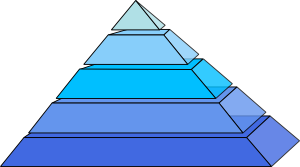
\includegraphics[width=1.1cm]{../Strukturfiler/FIGS/BluePyramid} & \begin{minipage}{\obsl}}{\end{minipage}\\ \end{tabular}\vspace{4mm}\newline}


% = Forudsætning = basis
\newenvironment{basis}{\begin{flushleft} \begin{itshape} }{\end{itshape} \end{flushleft}}


% = Opsummering =
\newenvironment{summary}{\clearpage\pagecolor{sumgul}\section{Opsummering}}{\newpage\pagecolor{white}}











% = Counter
\newcounter{opgavecount}[section]
\setcounter{opgavecount}{0}
\newcounter{spgcount}[opgavecount]
\setcounter{spgcount}{0}
\renewcommand{\thespgcount}{\alph{spgcount})}



% = EXERCISE = (DIVIDER)

\newcommand{\exercisebegin}[1][]{\bigskip\needspace{3\baselineskip}\refstepcounter{opgavecount}\titlegraphic{mingroen}\textcolor{mingroen}{\th{Opgave \theopgavecount \hspace*{1cm} #1}}\medskip\par}

% = QUIZEXERCISE = (DIVIDER)

\newcommand{\quizexercisebegin}[1][]{\bigskip\needspace{3\baselineskip}\refstepcounter{opgavecount}\titlegraphic{mingroen}\textcolor{mingroen}{\th{Quiz-Opgave \theopgavecount \hspace*{1cm} #1}}\medskip\par}

% = QUESTION =

\newenvironment{question}{\refstepcounter{spgcount}\begin{itemize}\item[\thespgcount]}{\end{itemize}\hspace*{\fill}}

% = VINK =

\newenvironment{vink}{\begin{tabular}{m{.9cm}<{\hspace*{2mm}}@{}|m{\obsl}@{}}\hspace*{-4pt}\raggedleft
\includegraphics[width=.9cm]{../Strukturfiler/FIGS/Think} & \begin{minipage}{\obsl}}{\end{minipage}\\ \end{tabular}\medskip\\}
	
% = FACIT =

\newenvironment{facit}{\begin{tabular}{m{.9cm}<{\hspace*{2mm}}@{}|m{\obsl}@{}}\hspace*{-4pt}\raggedleft
\includegraphics[width=.9cm]{../Strukturfiler/FIGS/Check} & \begin{minipage}{\obsl}}{\end{minipage}\\ \end{tabular}\medskip\\}








\newcommand{\afsnit}[1]{\bigskip\th{\titlegraphic{mingroen}\textcolor{mingroen}{#1}} \\ \rule[7pt]{.4\textwidth}{1pt} \vspace*{-2.5mm}\par}

% (DIVIDER):
\newcommand{\ugedagdatotitel}[4]{\pagebreak[4]\section{Semesteruge #1 -- #2 Dag \hspace*{1mm} (#3)} \vspace*{-4mm} \rule[5pt]{\textwidth}{1pt}\vspace*{-2.5mm} \begin{center}\large{\th{#4}}\end{center} \fancyhead[C]{\th{Semesteruge #1}}}

\newenvironment{skema}[1]{\definecolor{shadecolor}{rgb}{0.96,.98, 1.0} \setlength{\FrameSep}{6pt} \renewcommand{\FrameHeightAdjust}{10pt} \vspace*{-4pt}\begin{shaded} \begin{tabular}{#1}}{\end{tabular} \end{shaded} \vspace*{-7pt}}


% ========================

% MAKROER

%\newenvironment{matr}[1][]{\hspace*{-.8mm}\left[\hspace*{-1mm}\begin{array}{#1}}{\end{array}\hspace*{-1mm}\right]\hspace*{-.8mm}}
\newcommand{\bevisslut}{\begin{scriptsize} \begin{flushright} $ \blacksquare $ \end{flushright} \end{scriptsize}}

\newcommand{\tref}[2]{\hyperref[#1]{#2 \ref*{#1}}}
\newcommand{\thref}[2]{\hyperref[#1]{#2}}

\newcommand{\refA}[1]{\colorbox{yellow}{\ref{#1}}}
\newcommand{\hrefA}[2]{\colorbox{yellow}{\href{#1}{#2}}}
\newcommand{\trefA}[2]{\colorbox{yellow}{\hyperref[#1]{#2 \ref*{#1}}}}
\newcommand{\threfA}[2]{\colorbox{yellow}{\hyperref[#1]{#2}}}

\newenvironment{matr}[1]{\hspace*{-.8mm}\begin{bmatrix}\hspace*{-1mm}\begin{array}{#1}}{\end{array}\hspace*{-1mm}\end{bmatrix}\hspace*{-.8mm}}
\newcommand{\transp}{\hspace*{-.6mm}^{\top}}

\newcommand{\maengde}[2]{\left\lbrace \hspace*{-1mm} \begin{array}{c|c} #1 & #2 \end{array} \hspace*{-1mm} \right\rbrace}

\newenvironment{eqnalign}[1]{\setlength{\arraycolsep}{1.3pt}\begin{equation}\begin{array}{#1}}{\end{array}\end{equation}\par}
\newcommand{\eqnl}{\setlength{\arraycolsep}{1.3pt}}

\newcommand{\matind}[3]{{_\mathrm{#1}\mathbf{#2}_\mathrm{#3}}}
\newcommand{\vekind}[2]{{_\mathrm{#1}\mathbf{#2}}}
\newcommand{\jac}[2]{{\mathrm{Jacobi}_\mathbf{#1} (#2)}}
\newcommand{\diver}[2]{{\mathrm{div}\mathbf{#1} (#2)}}
\newcommand{\rot}[1]{{\mathbf{rot}\mathbf{(#1)}}}

\newcommand{\am}{\mathrm{am}}
\newcommand{\gm}{\mathrm{gm}}
\newcommand{\E}{\mathrm{E}}
\newcommand{\Span}{\mathrm{span}}
\newcommand{\mU}{\mathbf{U}}

\newcommand{\ms}{\medskip\\}
\newcommand{\bs}{\bigskip\\}

\newcommand{\mA}{\mathbf{A}}
\newcommand{\mB}{\mathbf{B}}
\newcommand{\mC}{\mathbf{C}}
\newcommand{\mD}{\mathbf{D}}
\newcommand{\mE}{\mathbf{E}}
\newcommand{\mF}{\mathbf{F}}
\newcommand{\mK}{\mathbf{K}}
\newcommand{\mI}{\mathbf{I}}
\newcommand{\mM}{\mathbf{M}}
\newcommand{\mN}{\mathbf{N}}
\newcommand{\mQ}{\mathbf{Q}}
\newcommand{\mT}{\mathbf{T}}
\newcommand{\mV}{\mathbf{V}}
\newcommand{\mW}{\mathbf{W}}
\newcommand{\mX}{\mathbf{X}}
\newcommand{\ma}{\mathbf{a}}
\newcommand{\mb}{\mathbf{b}}
\newcommand{\mc}{\mathbf{c}}
\newcommand{\md}{\mathbf{d}}
\newcommand{\me}{\mathbf{e}}
\newcommand{\mn}{\mathbf{n}}
\newcommand{\mr}{\mathbf{r}}
\newcommand{\mv}{\mathbf{v}}
\newcommand{\mw}{\mathbf{w}}
\newcommand{\mx}{\mathbf{x}}
\newcommand{\mxb}{\mathbf{x_{bet}}}
\newcommand{\my}{\mathbf{y}}
\newcommand{\mz}{\mathbf{z}}
\newcommand{\reel}{\mathbb{R}}
\newcommand{\mL}{\bm{\Lambda}} %Lambda-matrix
\newcommand{\mnul}{\bm{0}}
\newcommand{\trap}[1]{\mathrm{trap}(#1)}
\newcommand{\Det}{\operatorname{Det}}
\newcommand{\adj}{\operatorname{adj}}
\newcommand{\Ar}{\operatorname{Areal}}
\newcommand{\Vol}{\operatorname{Vol}}
\newcommand{\Rum}{\operatorname{Rum}}
\newcommand{\diag}{\operatorname{\bf{diag}}}
\newcommand{\bidiag}{\operatorname{\bf{bidiag}}}
\newcommand{\spanVec}[1]{\mathrm{span}\{#1\}}
\newcommand{\Div}{\operatorname{Div}}
\newcommand{\Rot}{\operatorname{\mathbf{Rot}}}

\newcommand{\Jac}{\operatorname{Jacobi}}
\newcommand{\Tan}{\operatorname{Tan}}
\newcommand{\Ort}{\operatorname{Ort}}
\newcommand{\Flux}{\operatorname{Flux}}
\newcommand{\Cmass}{\operatorname{Cm}}
\newcommand{\Imom}{\operatorname{Im}}
\newcommand{\Pmom}{\operatorname{Pm}}
\newcommand{\IS}{\operatorname{I}}
\newcommand{\IIS}{\operatorname{II}}
\newcommand{\IIIS}{\operatorname{III}}
\newcommand{\Le}{\operatorname{L}}
\newcommand{\app}{\operatorname{app}}
\newcommand{\M}{\operatorname{M}}
\newcommand{\re}{\mathrm{Re}}
\newcommand{\im}{\mathrm{Im}}

\newcommand{\compl}{\mathbb{C}} %de komplekse tal
\newcommand{\e}{\mathrm{e}} %eksponentialfunktionen. lodret 'e', og altså ikke kursiv ligesom andre bogstaver.





% Medialink: SCREEN: (QRcode) + thumbnail image + link på kodenummer (til qr.dtu.dk)
\newcommand{\onlinemedia}[3]{
	\begin{wrapfigure}{r}{3.2cm} 
		\vspace{-30pt} 
		\vspace{#1pt} 
		\begin{flushright} 
			\includegraphics[width=3cm]{qr/#2.png} 
			\tiny 
			\href{http://qr.dtu.dk/#2}{#2: #3}
			\normalsize  
		\end{flushright} 
		\vspace{-10pt} 
	\end{wrapfigure}
}
\newcommand{\onlinemediathumb}[3]{
	\begin{wrapfigure}{r}{3.2cm} 
		\vspace{-30pt} 
		\vspace{#1pt} 
		\begin{flushright} 
			\includegraphics[width=3cm]{qr/#2.png} 
			\includegraphics[width=3cm]{qr/#2_thumb.png} 
			\tiny 
			\href{http://qr.dtu.dk/#2}{#2: #3}
			\normalsize  
		\end{flushright} 
		\vspace{-10pt} 
	\end{wrapfigure}
}



% Index:
\usepackage{makeidx}
\makeindex
\newcommand\ind[2]{\index{#1}\textbf{\textit{\textcolor{black}{#2}}}}

% ###SERVER_EXCLUDE_BEGIN###
\externaldocument[NUID17-]{../../enoten/TN01-Talrum/Talrum}
\externaldocument[NUID1-]{../../enoten/TN02-Ligningssystemer/TNdriver}
\externaldocument[NUID2-]{../../enoten/TN03-Matricer_og_Matrixalgebra/Matricer_og_matrixalgebra}
\externaldocument[NUID3-]{../../enoten/TN04-Kvadratiske_matricer/TNdriver}
\externaldocument[NUID11-]{../../enoten/TN05-Determinanter/Determinanter}
\externaldocument[NUID12-]{../../enoten/TN06-GeometriskeVektorer/GeometriskeVektorer}
\externaldocument[NUID18-]{../../enoten/TN07-Vektorrum/VektorRum}
\externaldocument[NUID21-]{../../enoten/TN08-LinAfbildninger/LinAfbildninger}
\externaldocument[NUID23-]{../../enoten/TN09-Egenvaerdier_og_egenvektorer/TNdriver}
\externaldocument[NUID24-]{../../enoten/TN10-Diagonalisering_med_egenvektorer/TNdriver}
\externaldocument[NUID10-]{../../enoten/TN11-1.ordens_differentialligninger/TNdriver}
\externaldocument[NUID13-]{../../enoten/TN12-1.ordens_differentialligningssystemer/TNdriver}
\externaldocument[NUID14-]{../../enoten/TN13-2.ordens_differentialligninger/TNdriver}
\externaldocument[NUID27-]{../../enoten/TN14-Elemenataere_funktioner/Elementaere_Funktioner}
\externaldocument[NUID28-]{../../enoten/TN15-Funktioner2Variable/Funktioner_To_Variable}
\externaldocument[NUID29-]{../../enoten/TN16-Gradienter_og_Tangentplaner/Gradienter_og_Tangentplaner}
\externaldocument[NUID32-]{../../enoten/TN17-Taylor_formler/Taylor_Formler}
\externaldocument[NUID33-]{../../enoten/TN18-Taylor_2Var/Taylor_2Var}
\externaldocument[NUID34-]{../../enoten/TN19-SymMat/SymmetriskeMatricer}
\externaldocument[NUID35-]{../../enoten/TN20-KegleSnit/Keglesnit}
\externaldocument[NUID36-]{../../enoten/TN21-Riemann_Integral/Riemann_01}
\externaldocument[NUID37-]{../../enoten/TN22-Plan_Int/Plan_Int_01}
\externaldocument[NUID39-]{../../enoten/TN23-Flade_Int/Flade_Rum_Int_01}
\externaldocument[NUID40-]{../../enoten/TN24-Vektorfelter/Vektorfelter_01}
\externaldocument[NUID41-]{../../enoten/TN25-Flux/Flux_02}
\externaldocument[NUID42-]{../../enoten/TN26-Gauss/Gauss_01}
\externaldocument[NUID128-]{../../enoten/TN27-Stokes/Stokes_01}
\externaldocument[NUID43-]{../../enoten/TN29-KomplekseTal/KomplekseTal}

\externaldocument[NUID6-]{../../E-math-opgaver/Opgaver/opgU123}
\externaldocument[NUID19-]{../../E-math-opgaver/Opgaver/opgU45}
\externaldocument[NUID20-]{../../E-math-opgaver/Opgaver/opgU678}
\externaldocument[NUID25-]{../../E-math-opgaver/Opgaver/opgU910SD}
\externaldocument[NUID31-]{../../E-math-opgaver/OpgaverF11-U123/opgF123}
% \externaldocument[NUID9-]{../../E-math-opgaver/Opgaver/Dagsordner E10}
% ###SERVER_EXCLUDE_END###


% Begin document and set alternative chapter title:
\begin{document}
\renewcommand{\chaptername}{eNote}

\setcounter{chapter}{22} %SÆT DETTE TAL TIL 1 MINDRE END DET AKTUELLE TRANSFERNOTE-NUMMER!!

%%%%%%%%%%%%%%%%%%%%%%%%%%%%%%%%%%%%%%%%%%%%%
%%%%%%%%%%%%%%%%%%%555%%%%%%%%%%%%%%%%%%%%%%%%%%
%%% HERFRA SKAL DU SKRIVE ELLER INDSÆTTE %%%%
%%% DEN FIL DU ØNSKER %%%%%%%%%%%%%%%%%%%%%%%
%%%%%%%%%%%%%%%%%%%%%%%%%%%%%%%%%%%%%%%%%%%%%
%%%%%%%%%%%%%%%%%%%%%%%%%%%%%%%%%%%%%%%%%%%%%


% REF: TransferNote \ref{TN4-tn4} \nameref{TN4-tn4}
%
% \tref{NUID14-thm.koma}{sætning} \tref{NUID28-tn15}{eNote}
%
%\tref{NUID34-tn19}{eNote} Symmetriske matricer
%\tref{NUID33-tn18}{eNote} Taylor i 2 variable
%
% 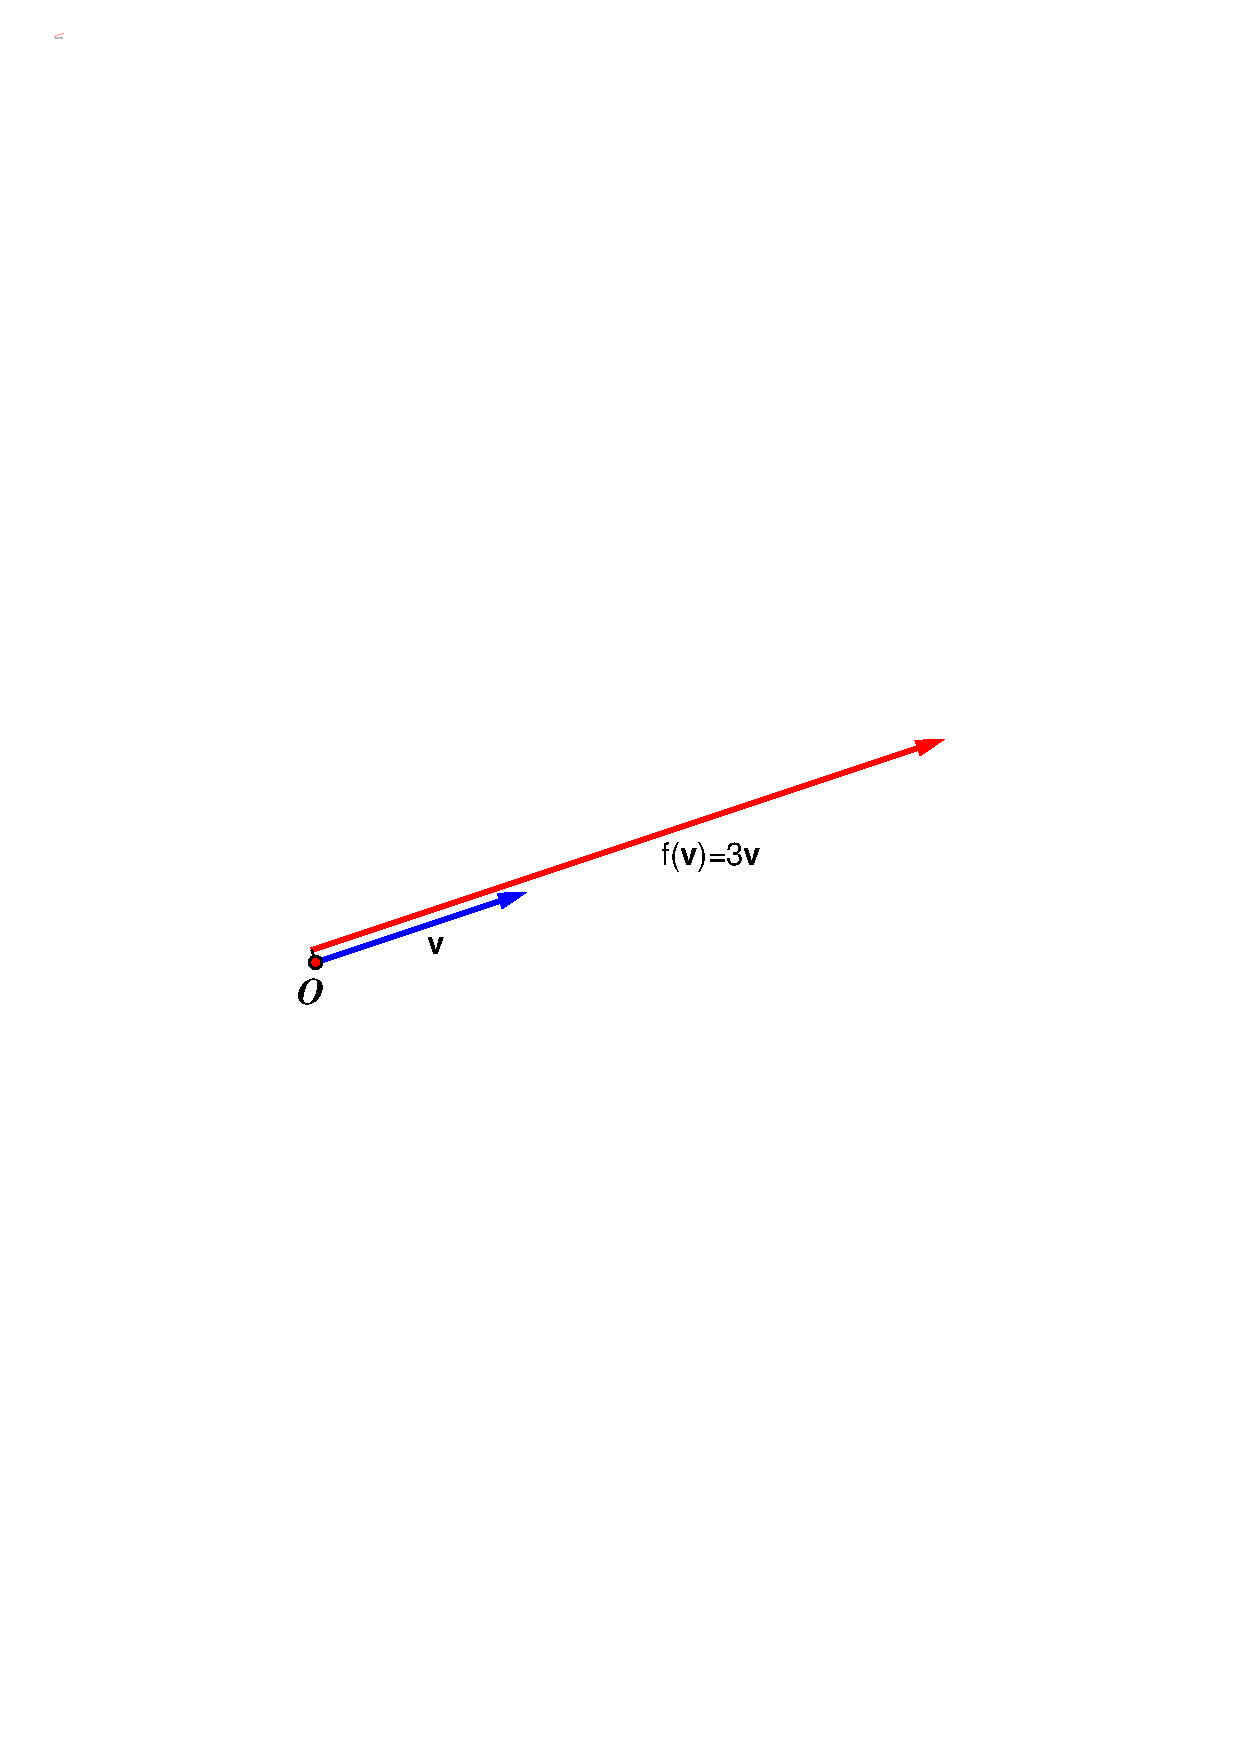
\includegraphics[trim=5cm 12cm 5cm 12cm,width=0.40\textwidth,clip]{skalering.pdf}
%
%\begin{equation}
%\matind vMa \cdot \matind aFa \cdot \matind aMv = \matind vFv \, ,
%\end{equation}
%hvor
%\begin{equation}
%\matind aMv = \begin{matr}{cccc} \vekind av_1 & \vekind av_2 & \cdots & \vekind av_n \end{matr} \quad \mathrm{og} \quad %\matind vFv = \diag(\lambda_1, \lambda_2, \ldots, \lambda_n) \, .
%\end{equation}
%
%$\vekind{e}{F}$
%$\matind{e}{F}{w}$
%
%\href{http://www-groups.dcs.st-and.ac.uk/~history/}{http://www-groups.dcs.st-and.ac.uk/~history/}

%%%%%%%%%%%%%%%%%%%%%%%%%%%%%%%%%%%%%%%%%%%%%%%%%%%
%%%%%%%%%%%%%%%%%%%%%%%%%%%%%%%%%%%%%%%%%%%%%%%%%%%
%%%%%%%%%%%%%%%%%%%%%%%%%%%%%%%%%%%%%%%%%%%%%%%%%%%
%%%%%%%%%%%%%%%%%%%%%%%%%%%%%%%%%%%%%%%%%%%%%%%%%%%

\chapter{Flade- og rum-integraler} \label{tn23}


\begin{basis}
Flade og rumintegraler opstilles her på stort set samme måde som kurve- og planintegralerne i
\tref{NUID37-tn22}{eNote}, som derved sammen med den grundlæggende generelle indførelse i Rie\-mann-\-inte\-gralerne
\tref{NUID36-tn21}{eNote} danner basis for nærværende eNote. Udgangspunktet for bestemmelse af flade- og rum-integralerne er fladernes og de rumlige områders respektive parameterfremstillinger. Til hver parameterfremstillling hører en Jacobi-funktion og det er denne funktion der benyttes til opstilling og beregning af integralerne.
\end{basis}



%%%%%%%%%%%%%%%%%%%%%%%%%%%%%%%%%%%%%%%%%%%%%%%%%%%
%%%%%%%%%%%%%%%%%%%%%%%%%%%%%%%%%%%%%%%%%%%%%%%%%%%
%%%%%%%%%%%%%%%%%%%%%%%%%%%%%%%%%%%%%%%%%%%%%%%%%%%
%%%%%%%%%%%%%%%%%%%%%%%%%%%%%%%%%%%%%%%%%%%%%%%%%%%





\section{Flade-integraler} \label{secFladeInt}



\begin{figure}[ht]
\centerline{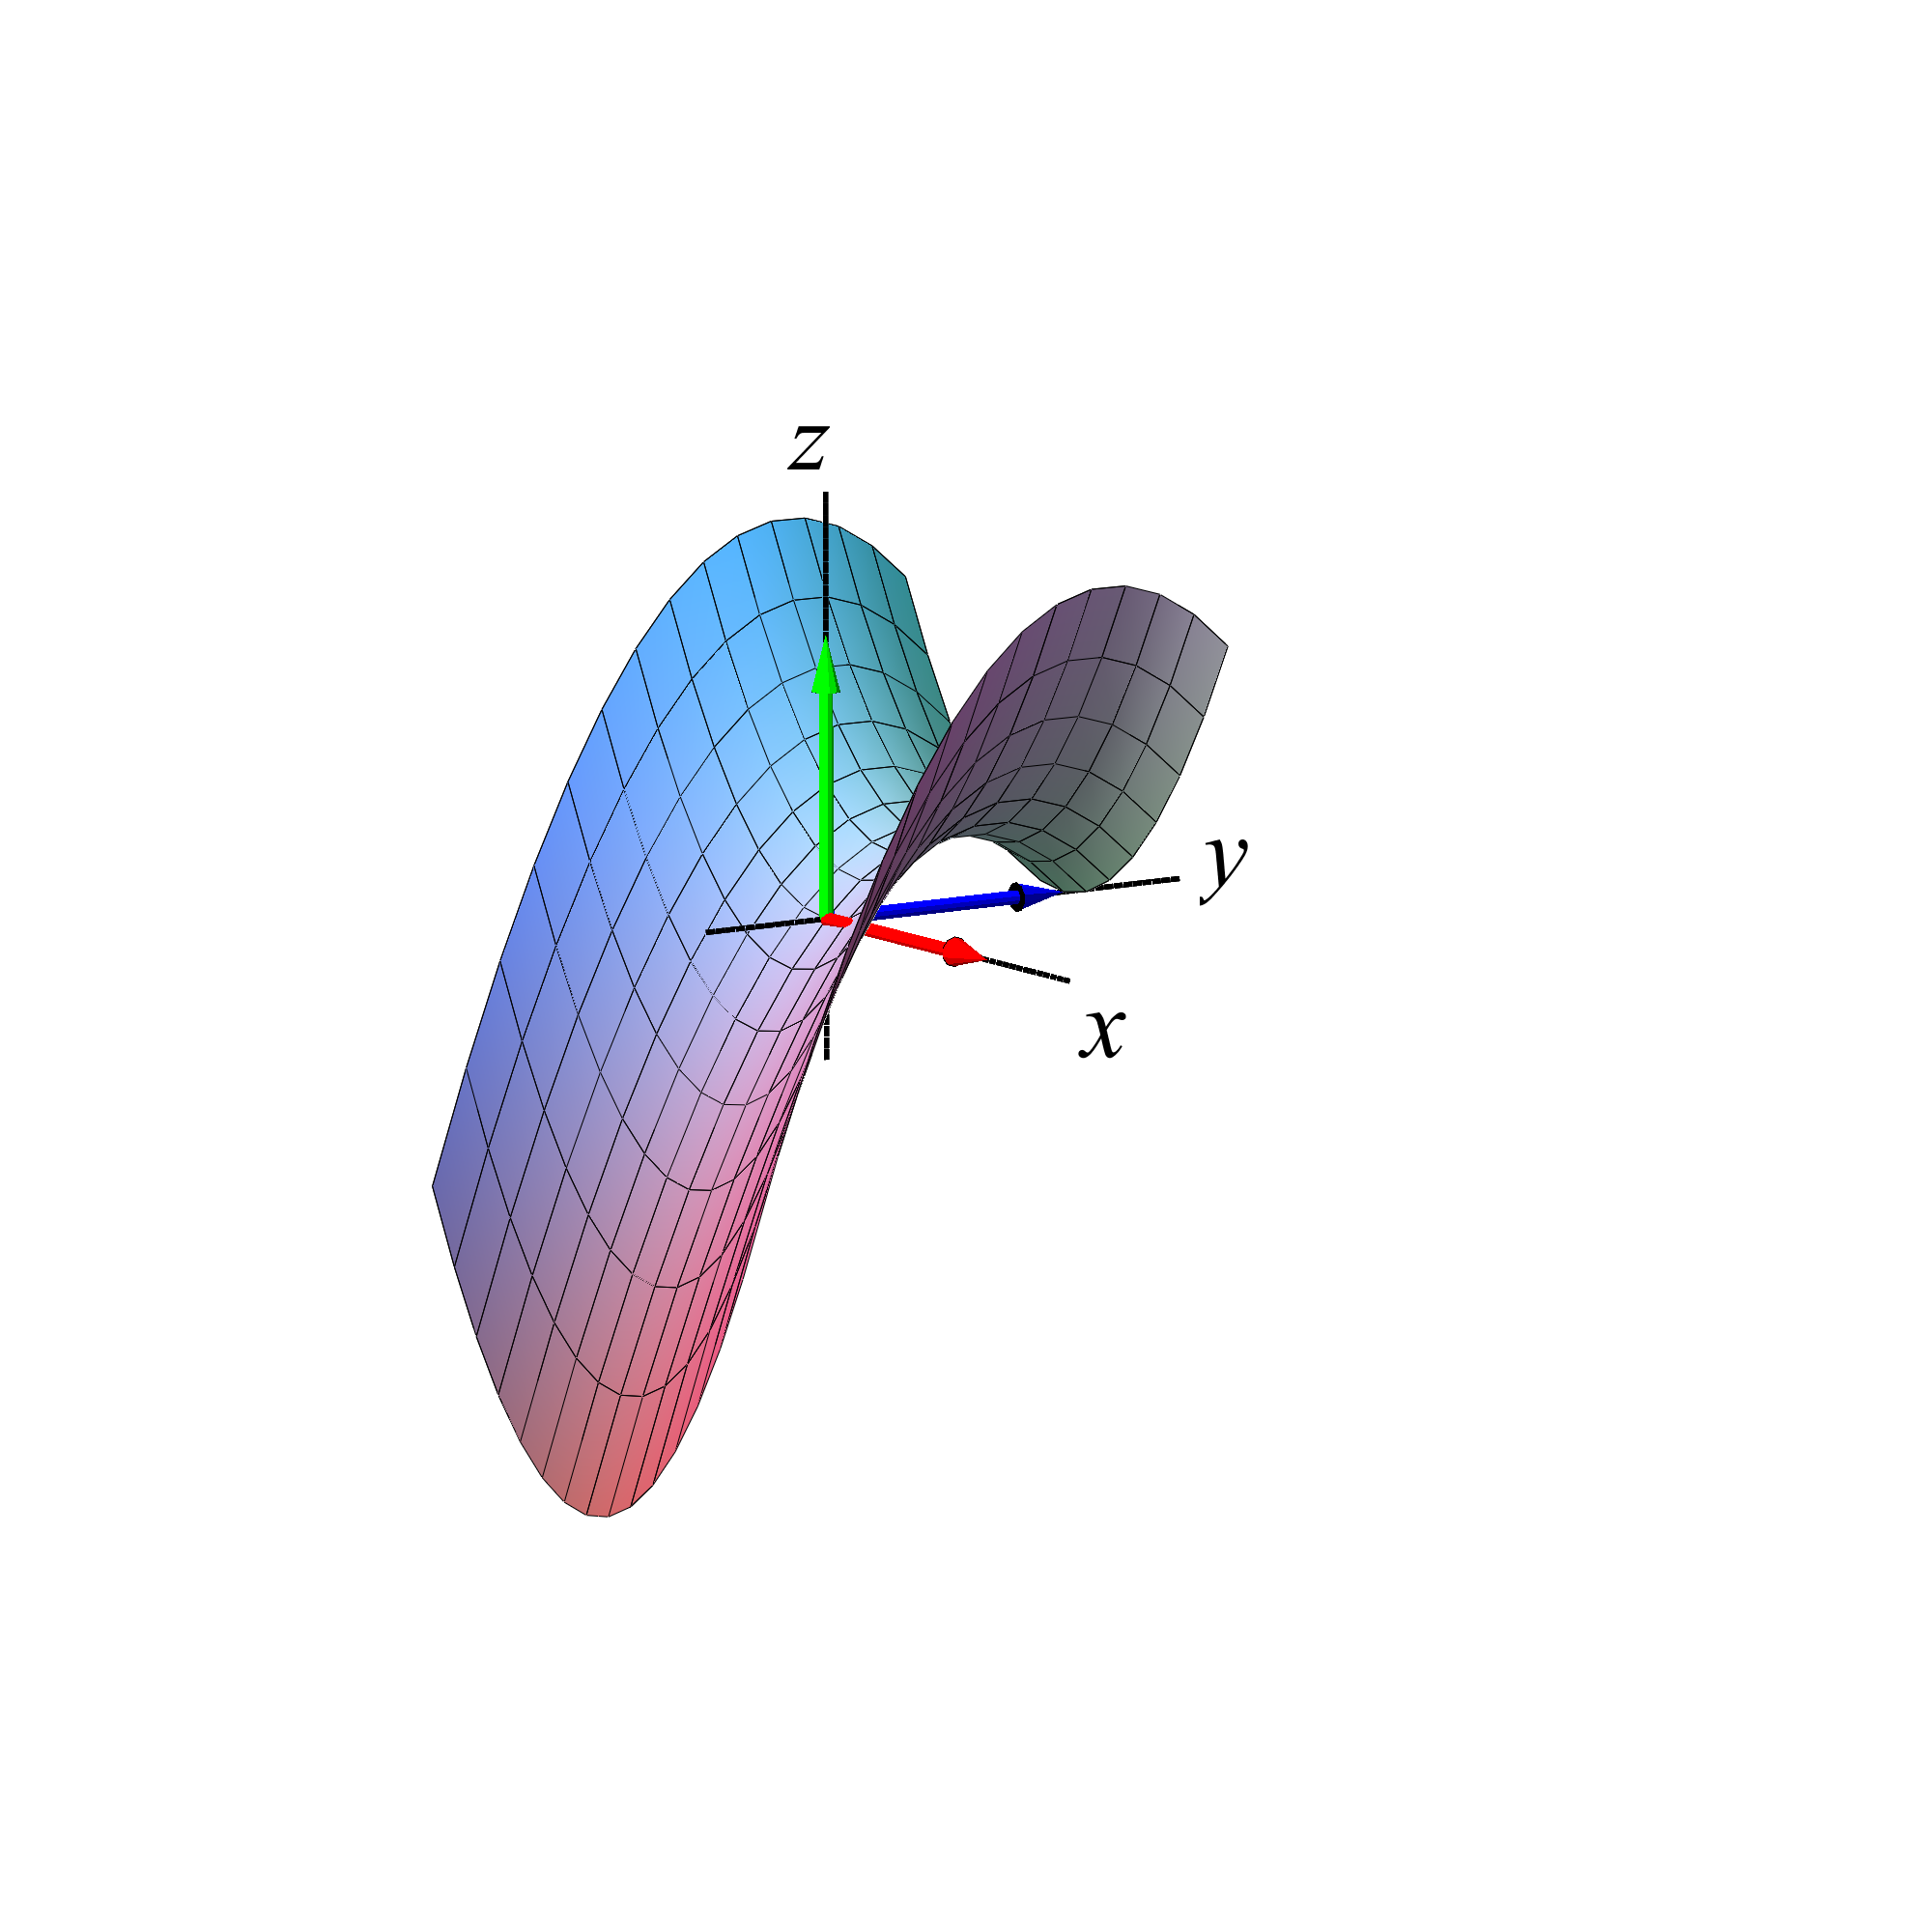
\includegraphics[height=75mm]{FIGS/plotGraf1} 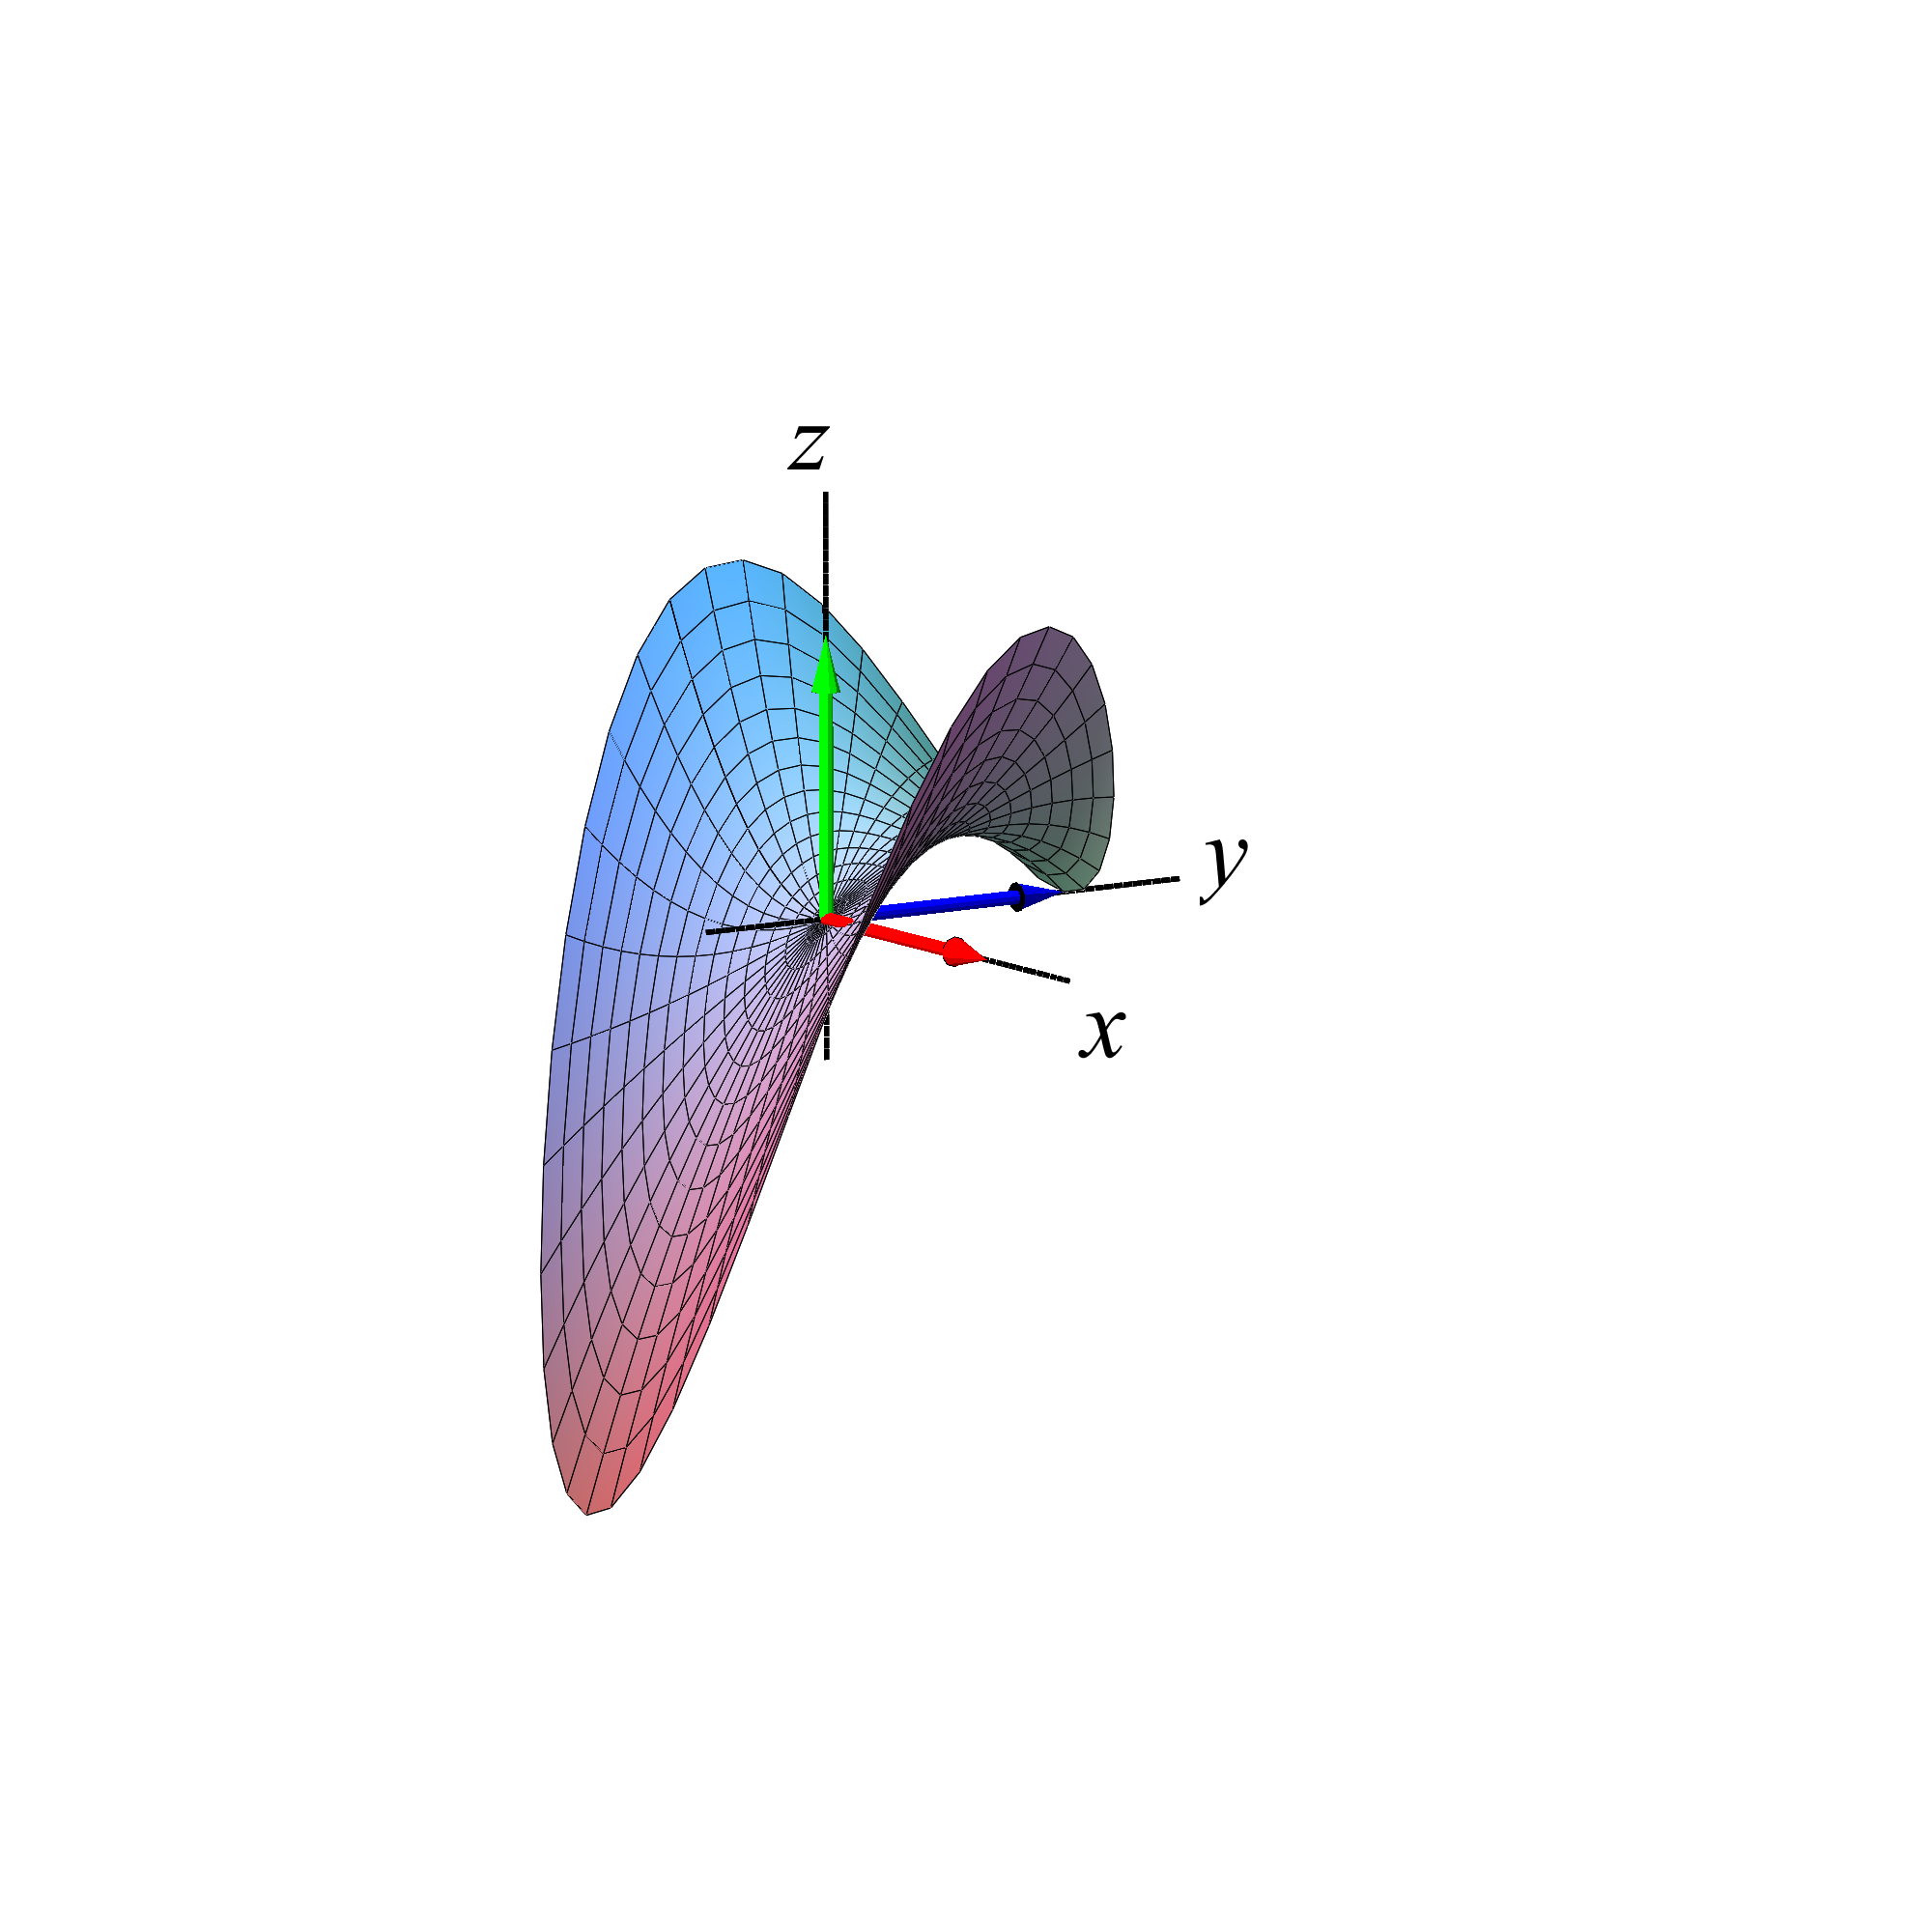
\includegraphics[height=75mm]{FIGS/plotGraf2}}
\begin{center}
\caption{\small{Graf-fladen for funktionen $h(x,y)= x^{2} - y^{2} + y$ dels over kvadratet $(x,y) \in [-1,1]\times [-1,1]$ og dels over cirkelskiven med radius $1$ og centrum i $(0, 0)$ i $((x,y))$-planen. }} \label{figGrafflade}
\end{center}
\end{figure}


En parametriseret {flade i rummet} er givet ved en
parameterfremstilling som meget lig\-ner parameterfremstillingerne for plane områder, jvf. \tref{NUID37-tn22}{eNote}.  Forskellen er dog den helt essentielle, at
her er også $z$-koordinaten en funktion af de to parameterværdier $u$ og $v$:
\begin{equation}
\label{eqFr}
F_{\bf r}: \quad {\bf r}(u,v) \, = \, \left(x(u,v), y(u,v),
z(u,v)\right) \in \mathbb{R}^3 \quad , \, \, \,  u \in [a,b] \, \,
, \, \,  v \in [c,d] \quad,
\end{equation}
hvor $x(u,v)$, $y(u,v)$, og $z(u,v)$ er givne glatte  funktioner af de to variable $u$ og $v$.


\begin{example}[Graf-flader for funktioner af to variable] \label{exampGrafflad}
En funktion $h(x,y)$  af to variable $(x,y) \in \mathbb{R}^{2}$ har en grafflade $\mathcal{F}$ i rummet, som let kan 'parametriseres' på den anviste form:
\begin{equation}
\mathcal{F} \quad : \quad \mathbf{r}(u,v) = (u, v, h(u,v)) \quad , \quad  u \in \mathbb{R} \, \,
, \, \,  v \in \mathbb{R} \quad.
\end{equation}
Typisk er vi kun interesserede i et udsnit af sådanne graf-flader, f.eks. det udsnit, der ligger over et rektangel i $(x,y)$ planen:
$x \in [a,b]$,
$ y \in [c,d]$. Det udsnit parametriseres lige så let som hele graffladen:
\begin{equation}
\widehat{\mathcal{F}} \quad : \quad \widehat{\mathbf{r}}(u,v) = (u, v, h(u,v)) \quad , \quad  \,  u \in [a,b] \, \,
, \, \,  v \in [c,d] \quad.
\end{equation}
Hvis vi derimod er interesserede i det udsnit af graffladen som ligger over cirkelskiven med radius $a$ og centrum i $(0,0)$ så må vi først  parametrisere cirkelskiven i $(x, y)$-planen med de to  parametre $u$ og $v$, hvorefter grafflade-udsnittet kan præsenteres ved at 'løfte' cirkelskive-punkterne til den kor\-rek\-te 'højde' med funktionen $h(x,y)$:
\begin{equation}
\widetilde{\mathcal{F}} \quad : \quad \widetilde{\mathbf{r}}(u,v) = \left(u\cdot \cos(v), u\cdot \sin(v), h\left(u\cdot \cos(v), u\cdot \sin(v)\right)\right) \quad ,
\end{equation}
hvor parametrene $u$ og $v$ nu gennemløber parameterområdet for cirkelskive-parametriseringen:
\begin{equation}
 u \in [0, a] \, \, \quad
, \, \, \quad  v \in [-\pi, \pi] \quad.
\end{equation}
\end{example}

I analogi med planintegralerne (jvf. \tref{NUID37-tn22}{eNote}) definerer vi nu fladeintegralerne således:

\begin{definition}[Fladeintegralet] \label{defFladeInt}
Lad $f(x,y,z)$ betegne en kontinuert funktion i $\mathbb{R}^{3}$.
Fladeintegralet af funktionen $f(x,y,z)$ over den parametriserede flade
$F_{\bf r}$ defineres ved
\begin{equation} \label{eqFladeintegral}
\int_{F_{\bf r}} f \, d\mu \, = \, \int_{c}^{d} \int_{a}^{b}
f({\bf r}(u,v))\, \Jac_{\bf r}(u,v)\,du \, dv \quad,
\end{equation}
hvor {Jacobi-funktionen  $\Jac_{\bf r}(u,v)$}
\begin{equation}
 \Jac_{\bf r}(u,v)\, = \,  | {\bf r}'_{u}(u,v) \times {\bf
 r}'_{v}(u,v) |  \quad
\end{equation}
er arealet af det parallelogram, der på stedet
${\bf r}(u,v)$ udspændes af de to tangentvektorer
${\bf r}'_{u}(u,v)$ og ${\bf
 r}'_{v}(u,v)$ til de respektive koordinatkurver igennem punktet
${\bf r}(u,v)$ på fladen.
\end{definition}


\begin{definition}[Regulær parameterfremstilling] \label{defRegFladeParam}
Parameterfremstillingen (\ref{eqFr}) siges at være en {\em{{regulær parameterfremstilling}}}
hvis der gælder følgende:
\begin{equation}
\Jac_{\bf r}(u,v)\, > 0 \quad \text{for alle} \quad  u \in [a,b] \, \,
, \, \,  v \in [c,d] \quad.
\end{equation}
\end{definition}


\begin{definition}[En-entydig parameterfremstilling]\label{defEnEntydFladeparam}
Som for parametriserede kurver siges parameterfremstillingen i
(\ref{eqFr}) at være \emph{en-entydig} hvis forskellige punkter i
definitionsmængden afbildes i forskellige punkter i billedmængden.
\end{definition}

\begin{figure}[ht]
\centerline{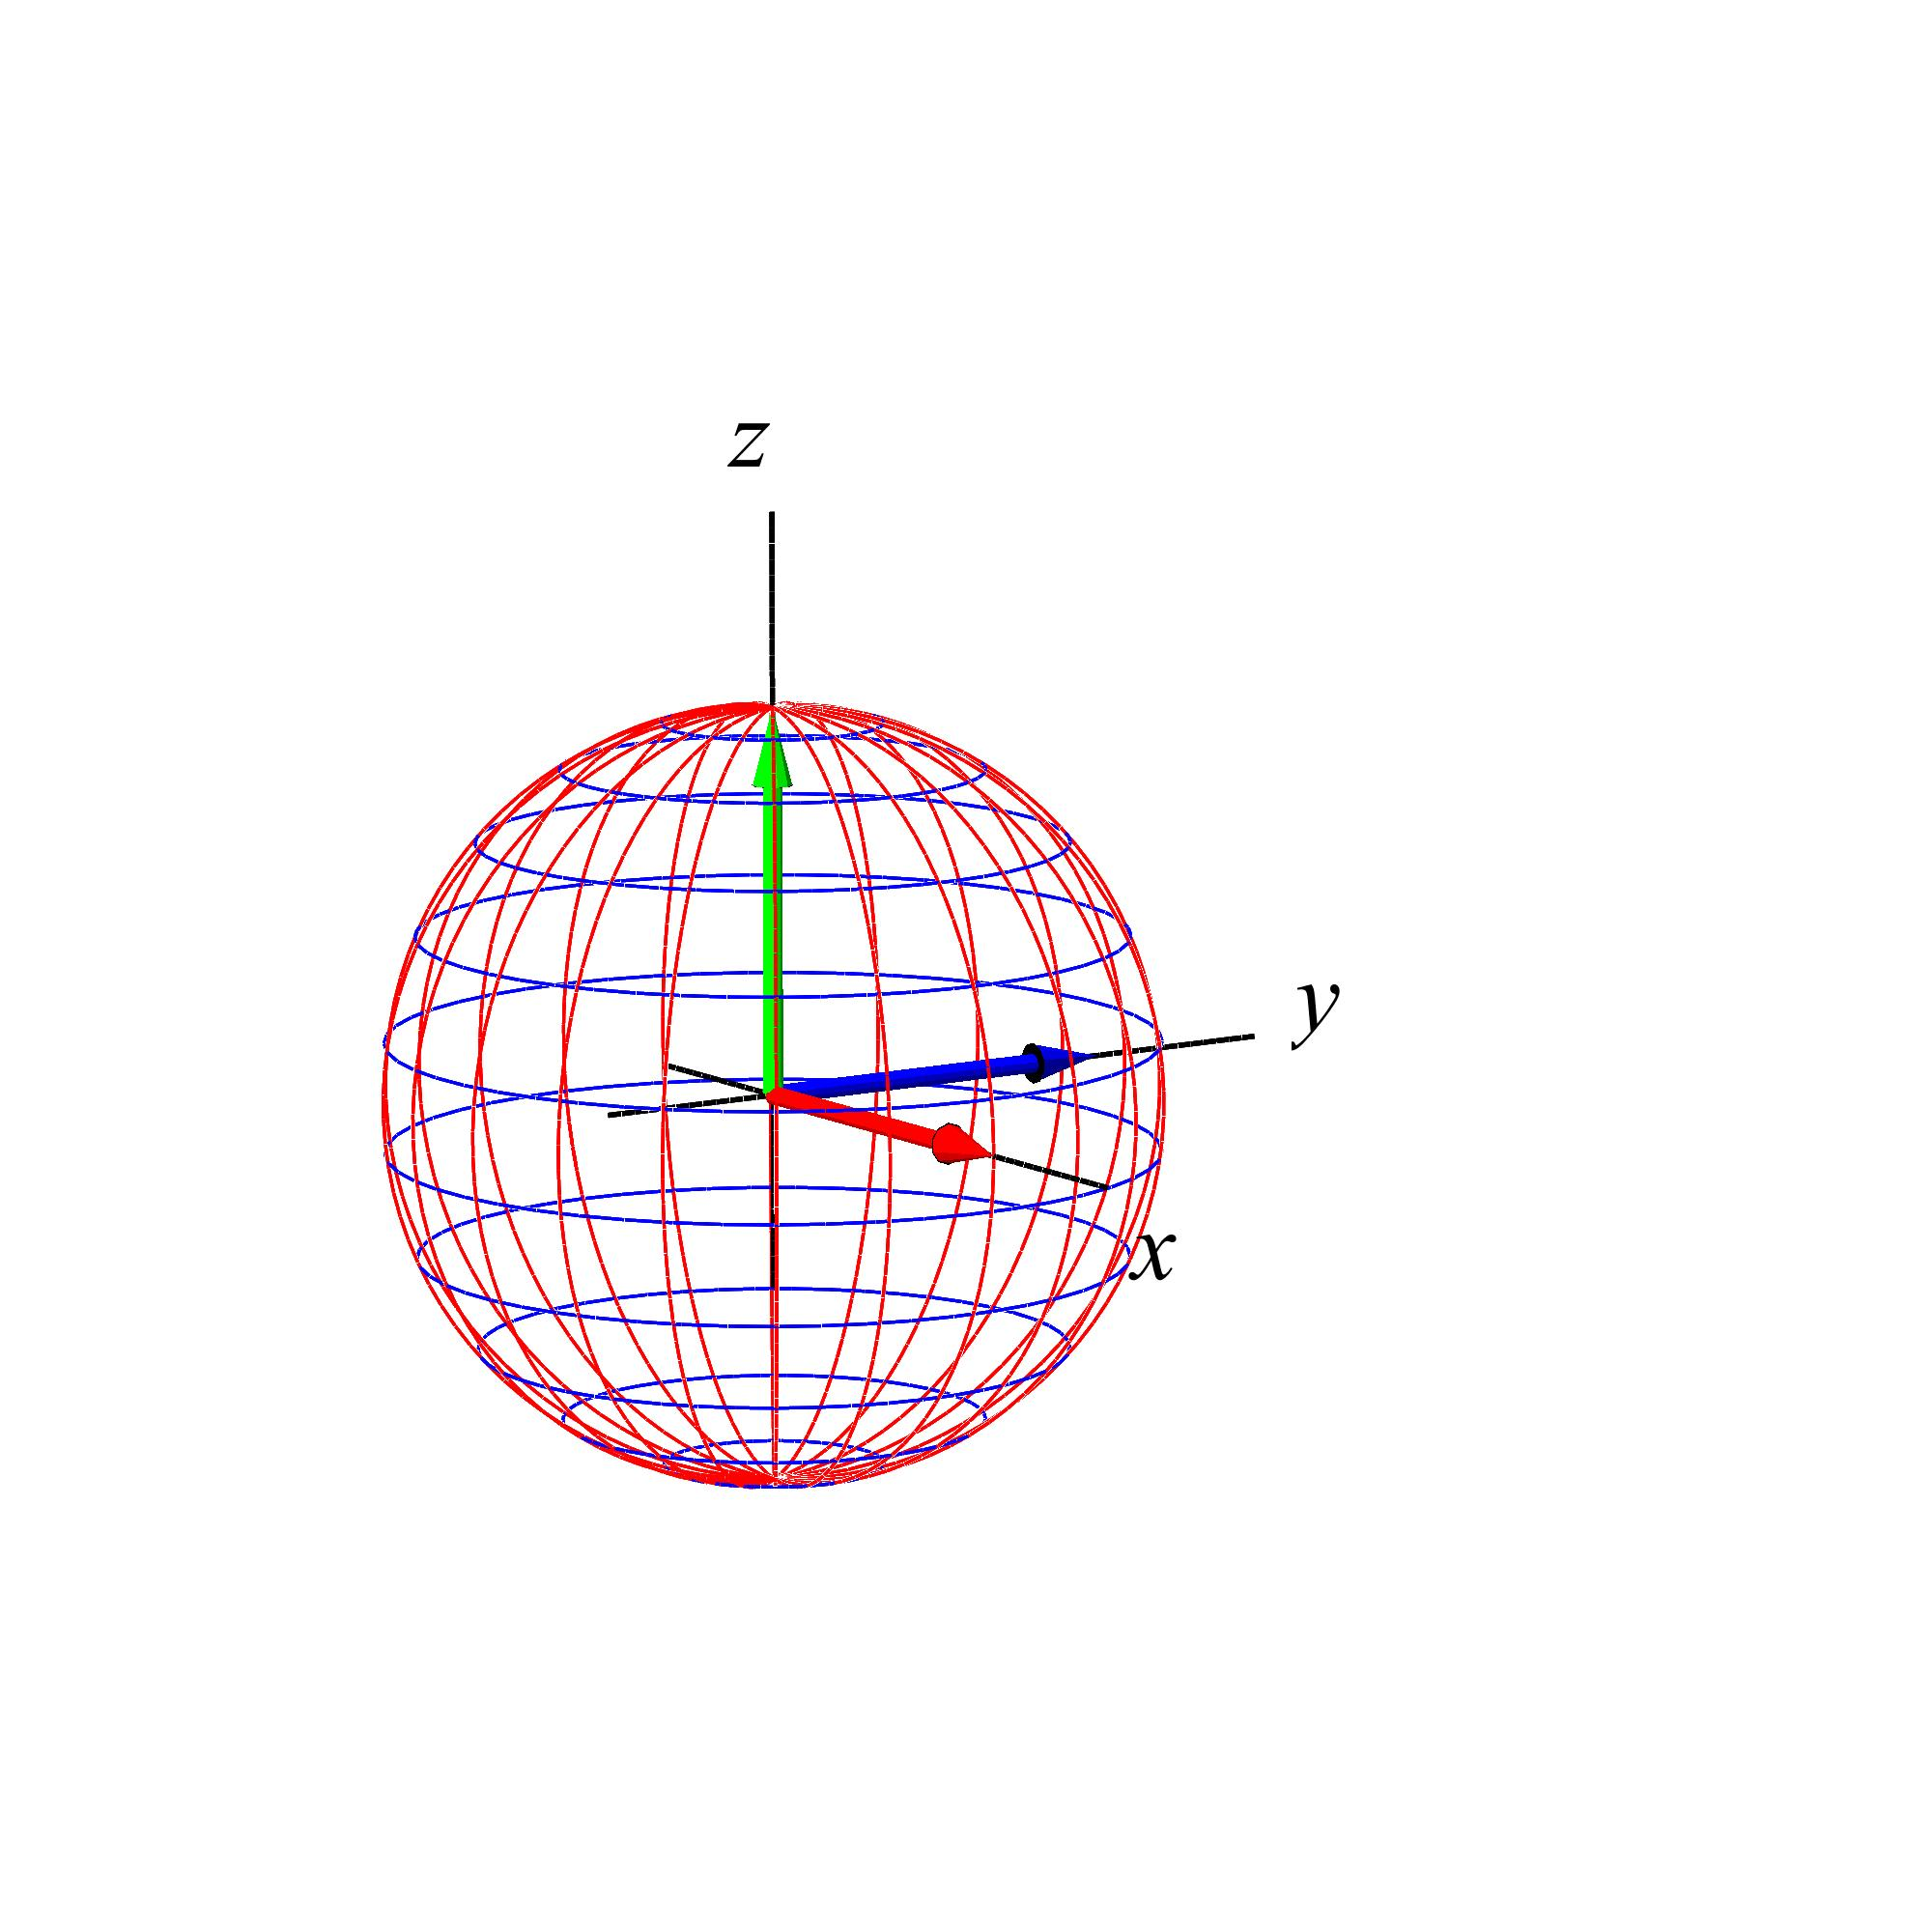
\includegraphics[height=30mm]{FIGS/plotKugWir1}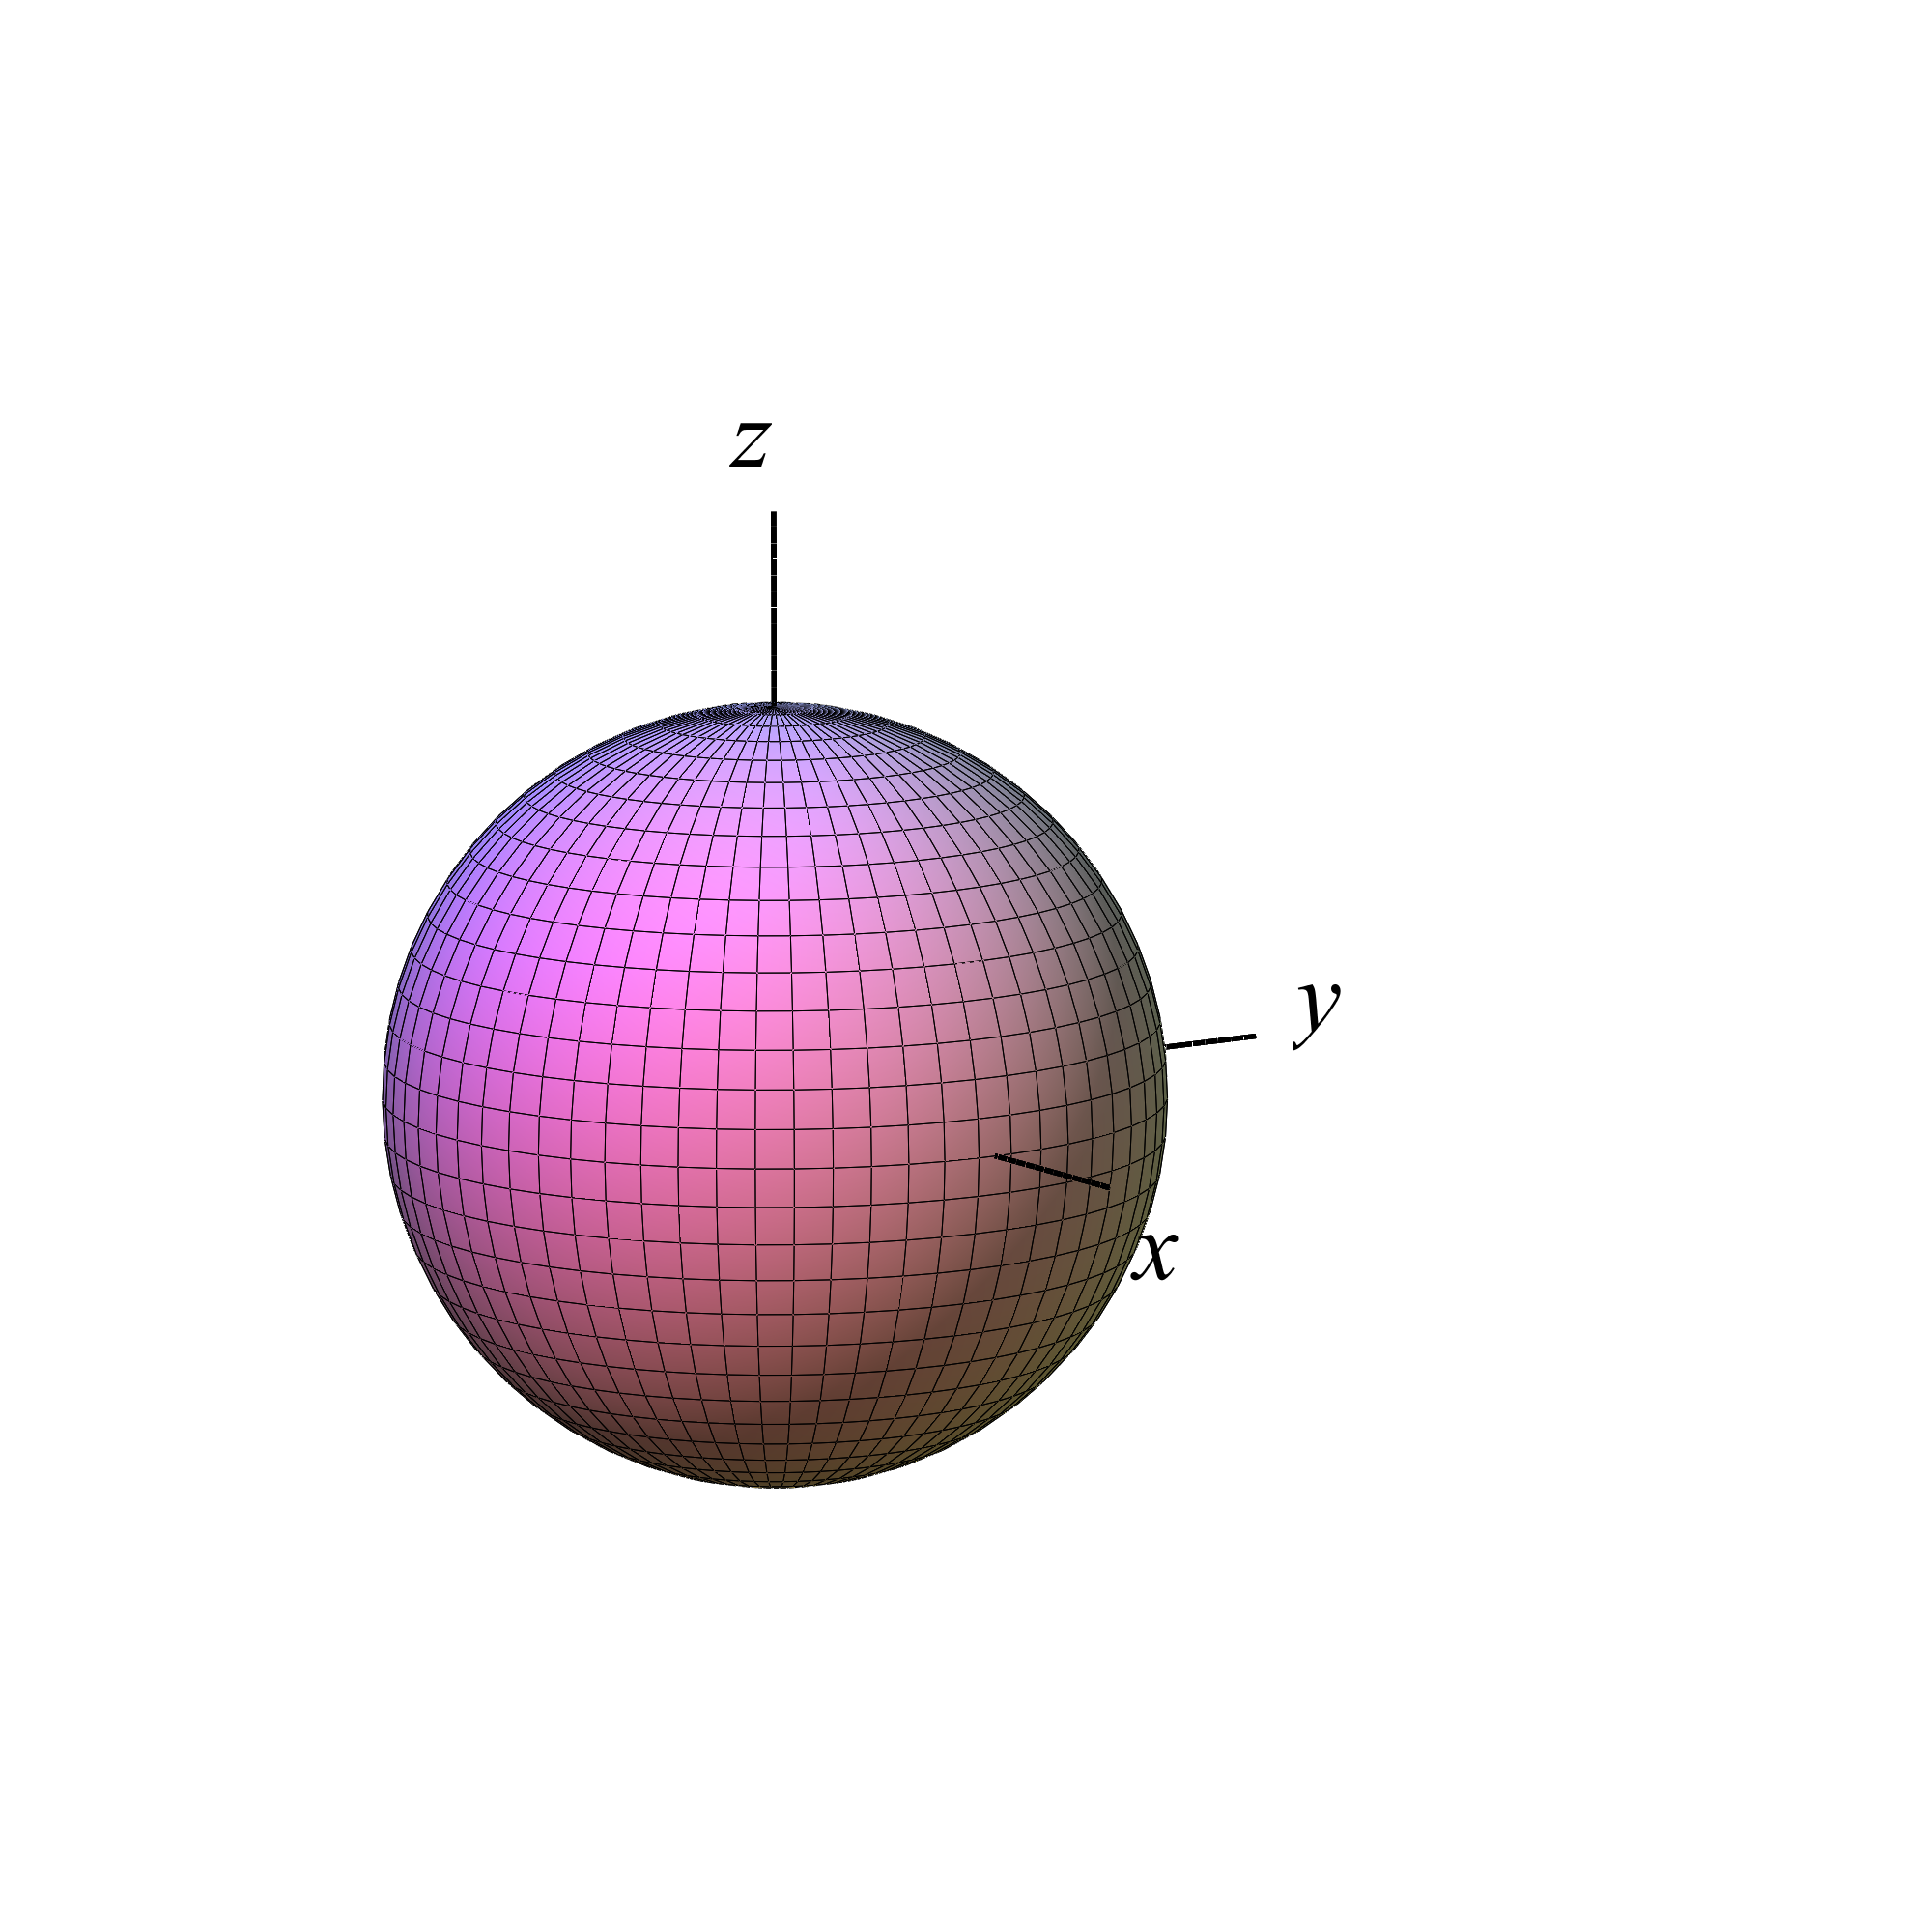
\includegraphics[height=50mm]{FIGS/plotKug1} \qquad \qquad 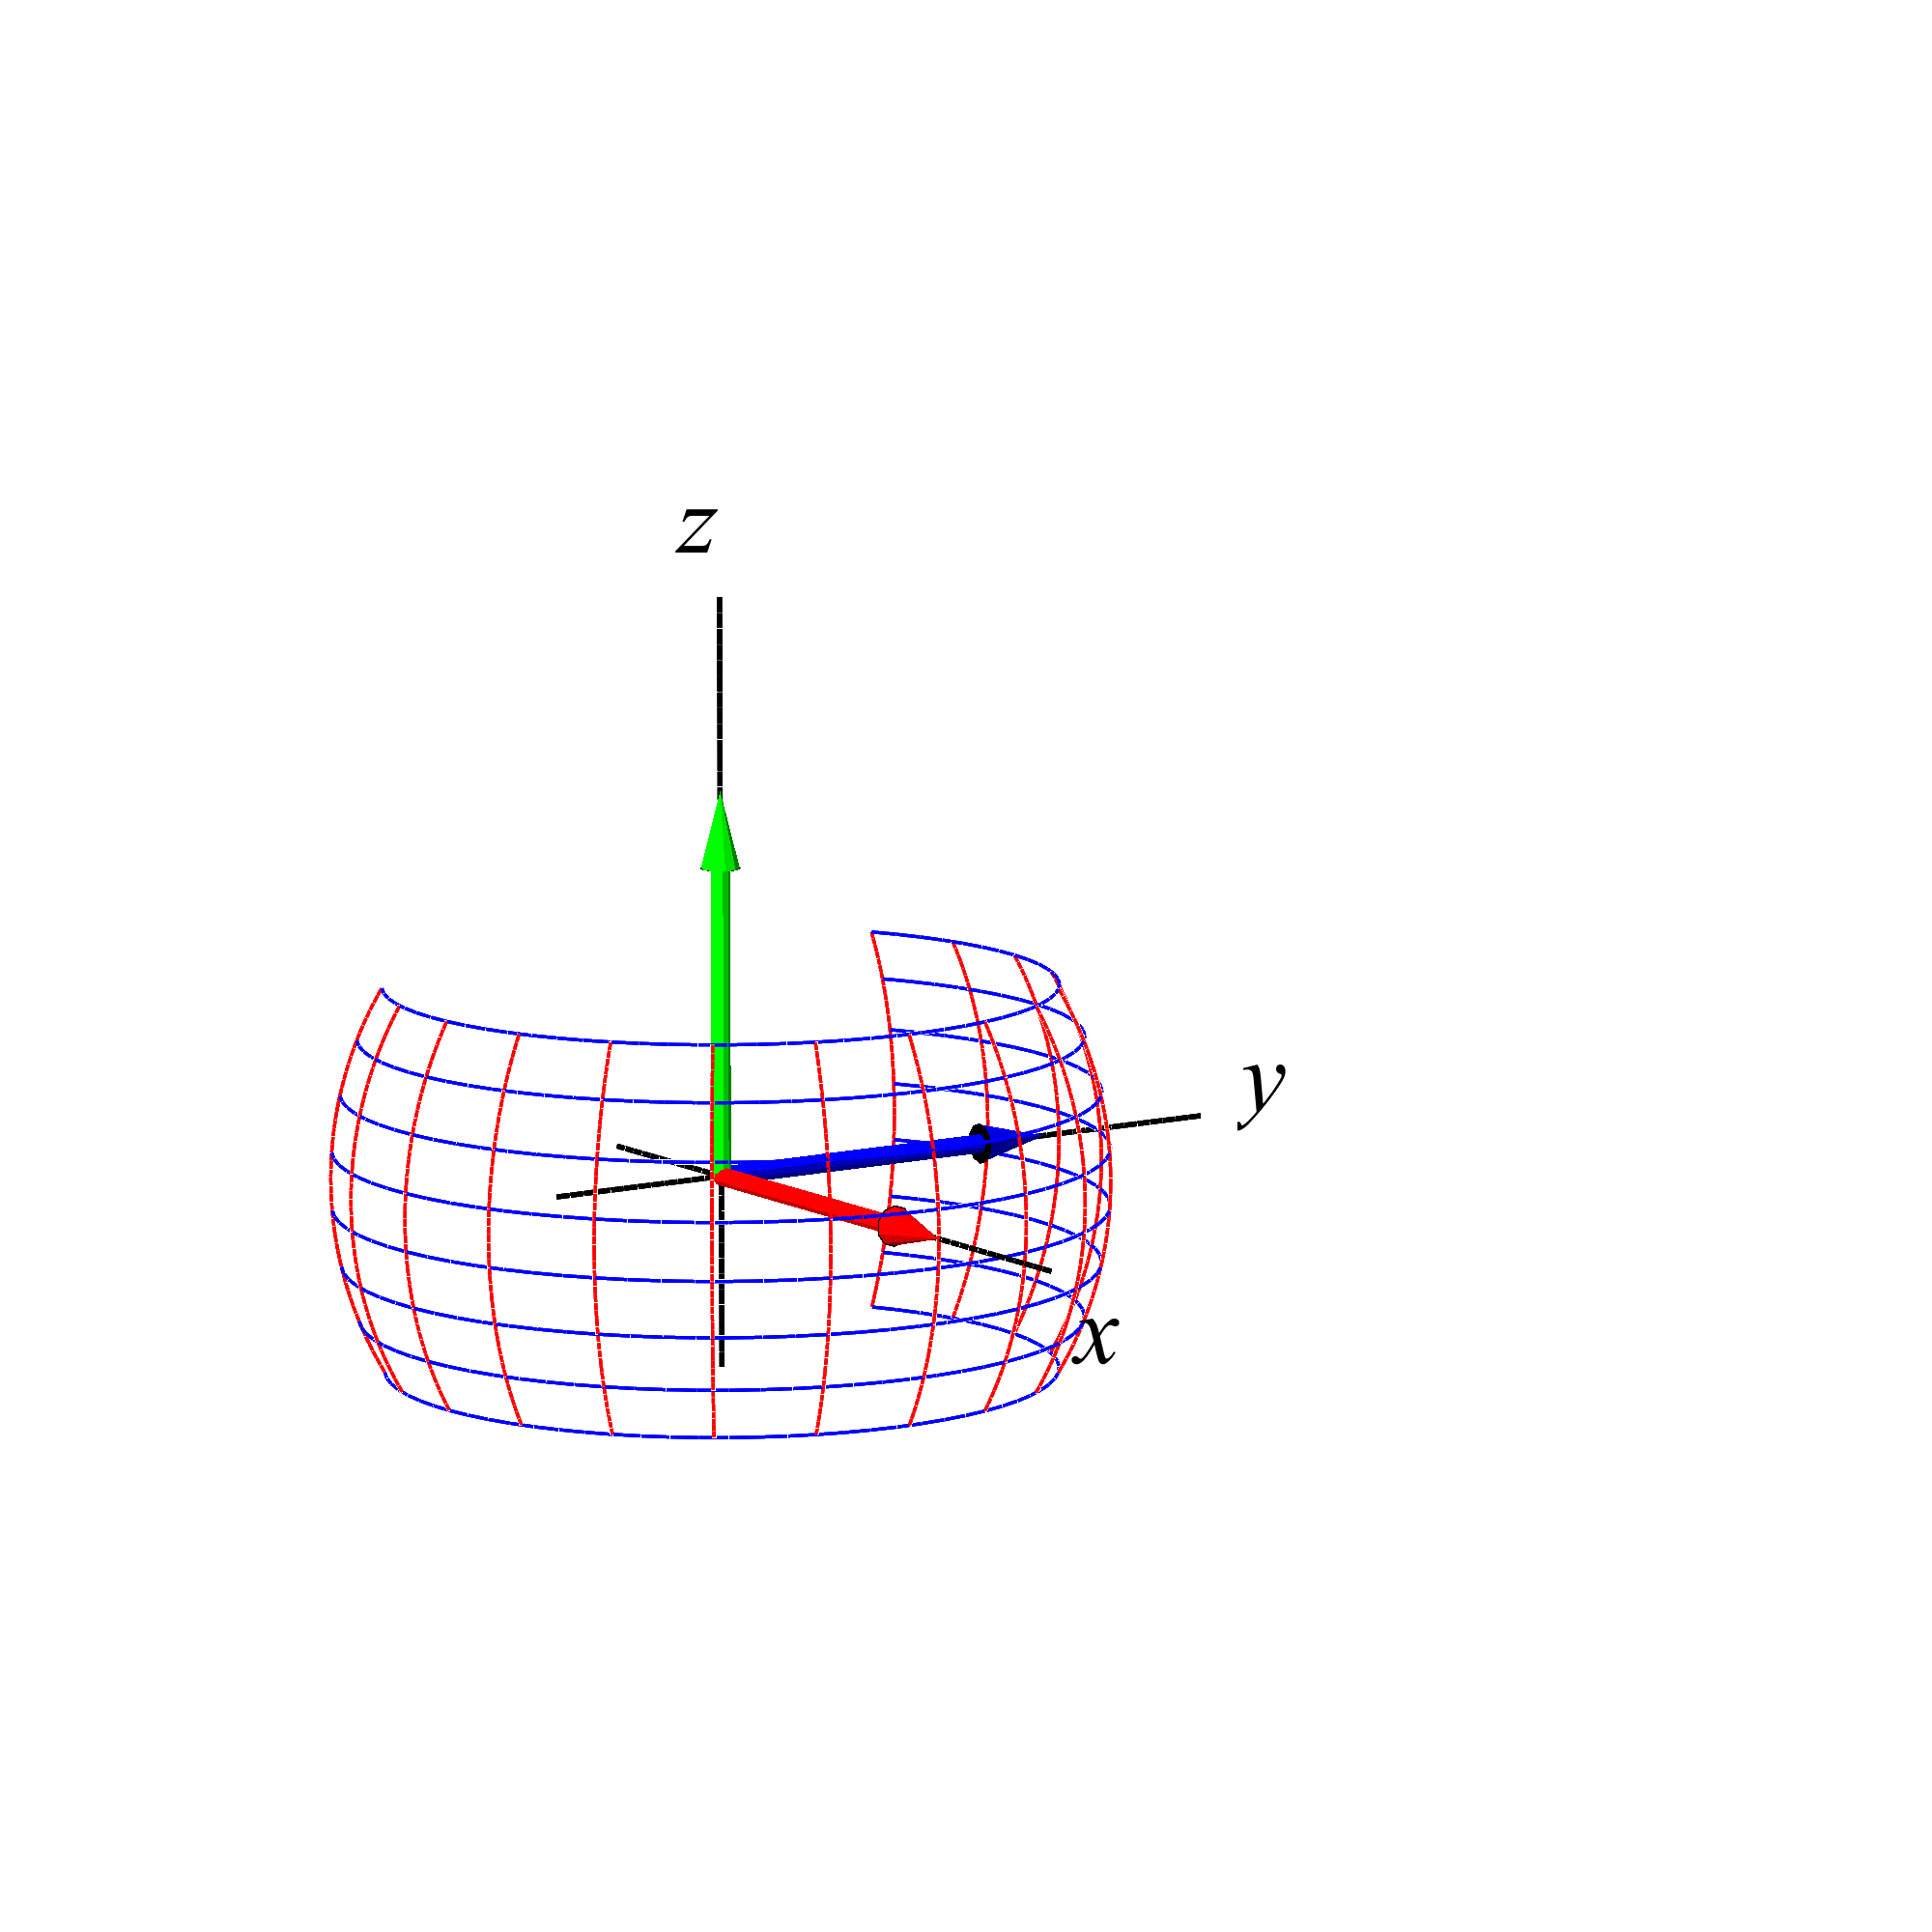
\includegraphics[height=30mm]{FIGS/plotKugWir2} 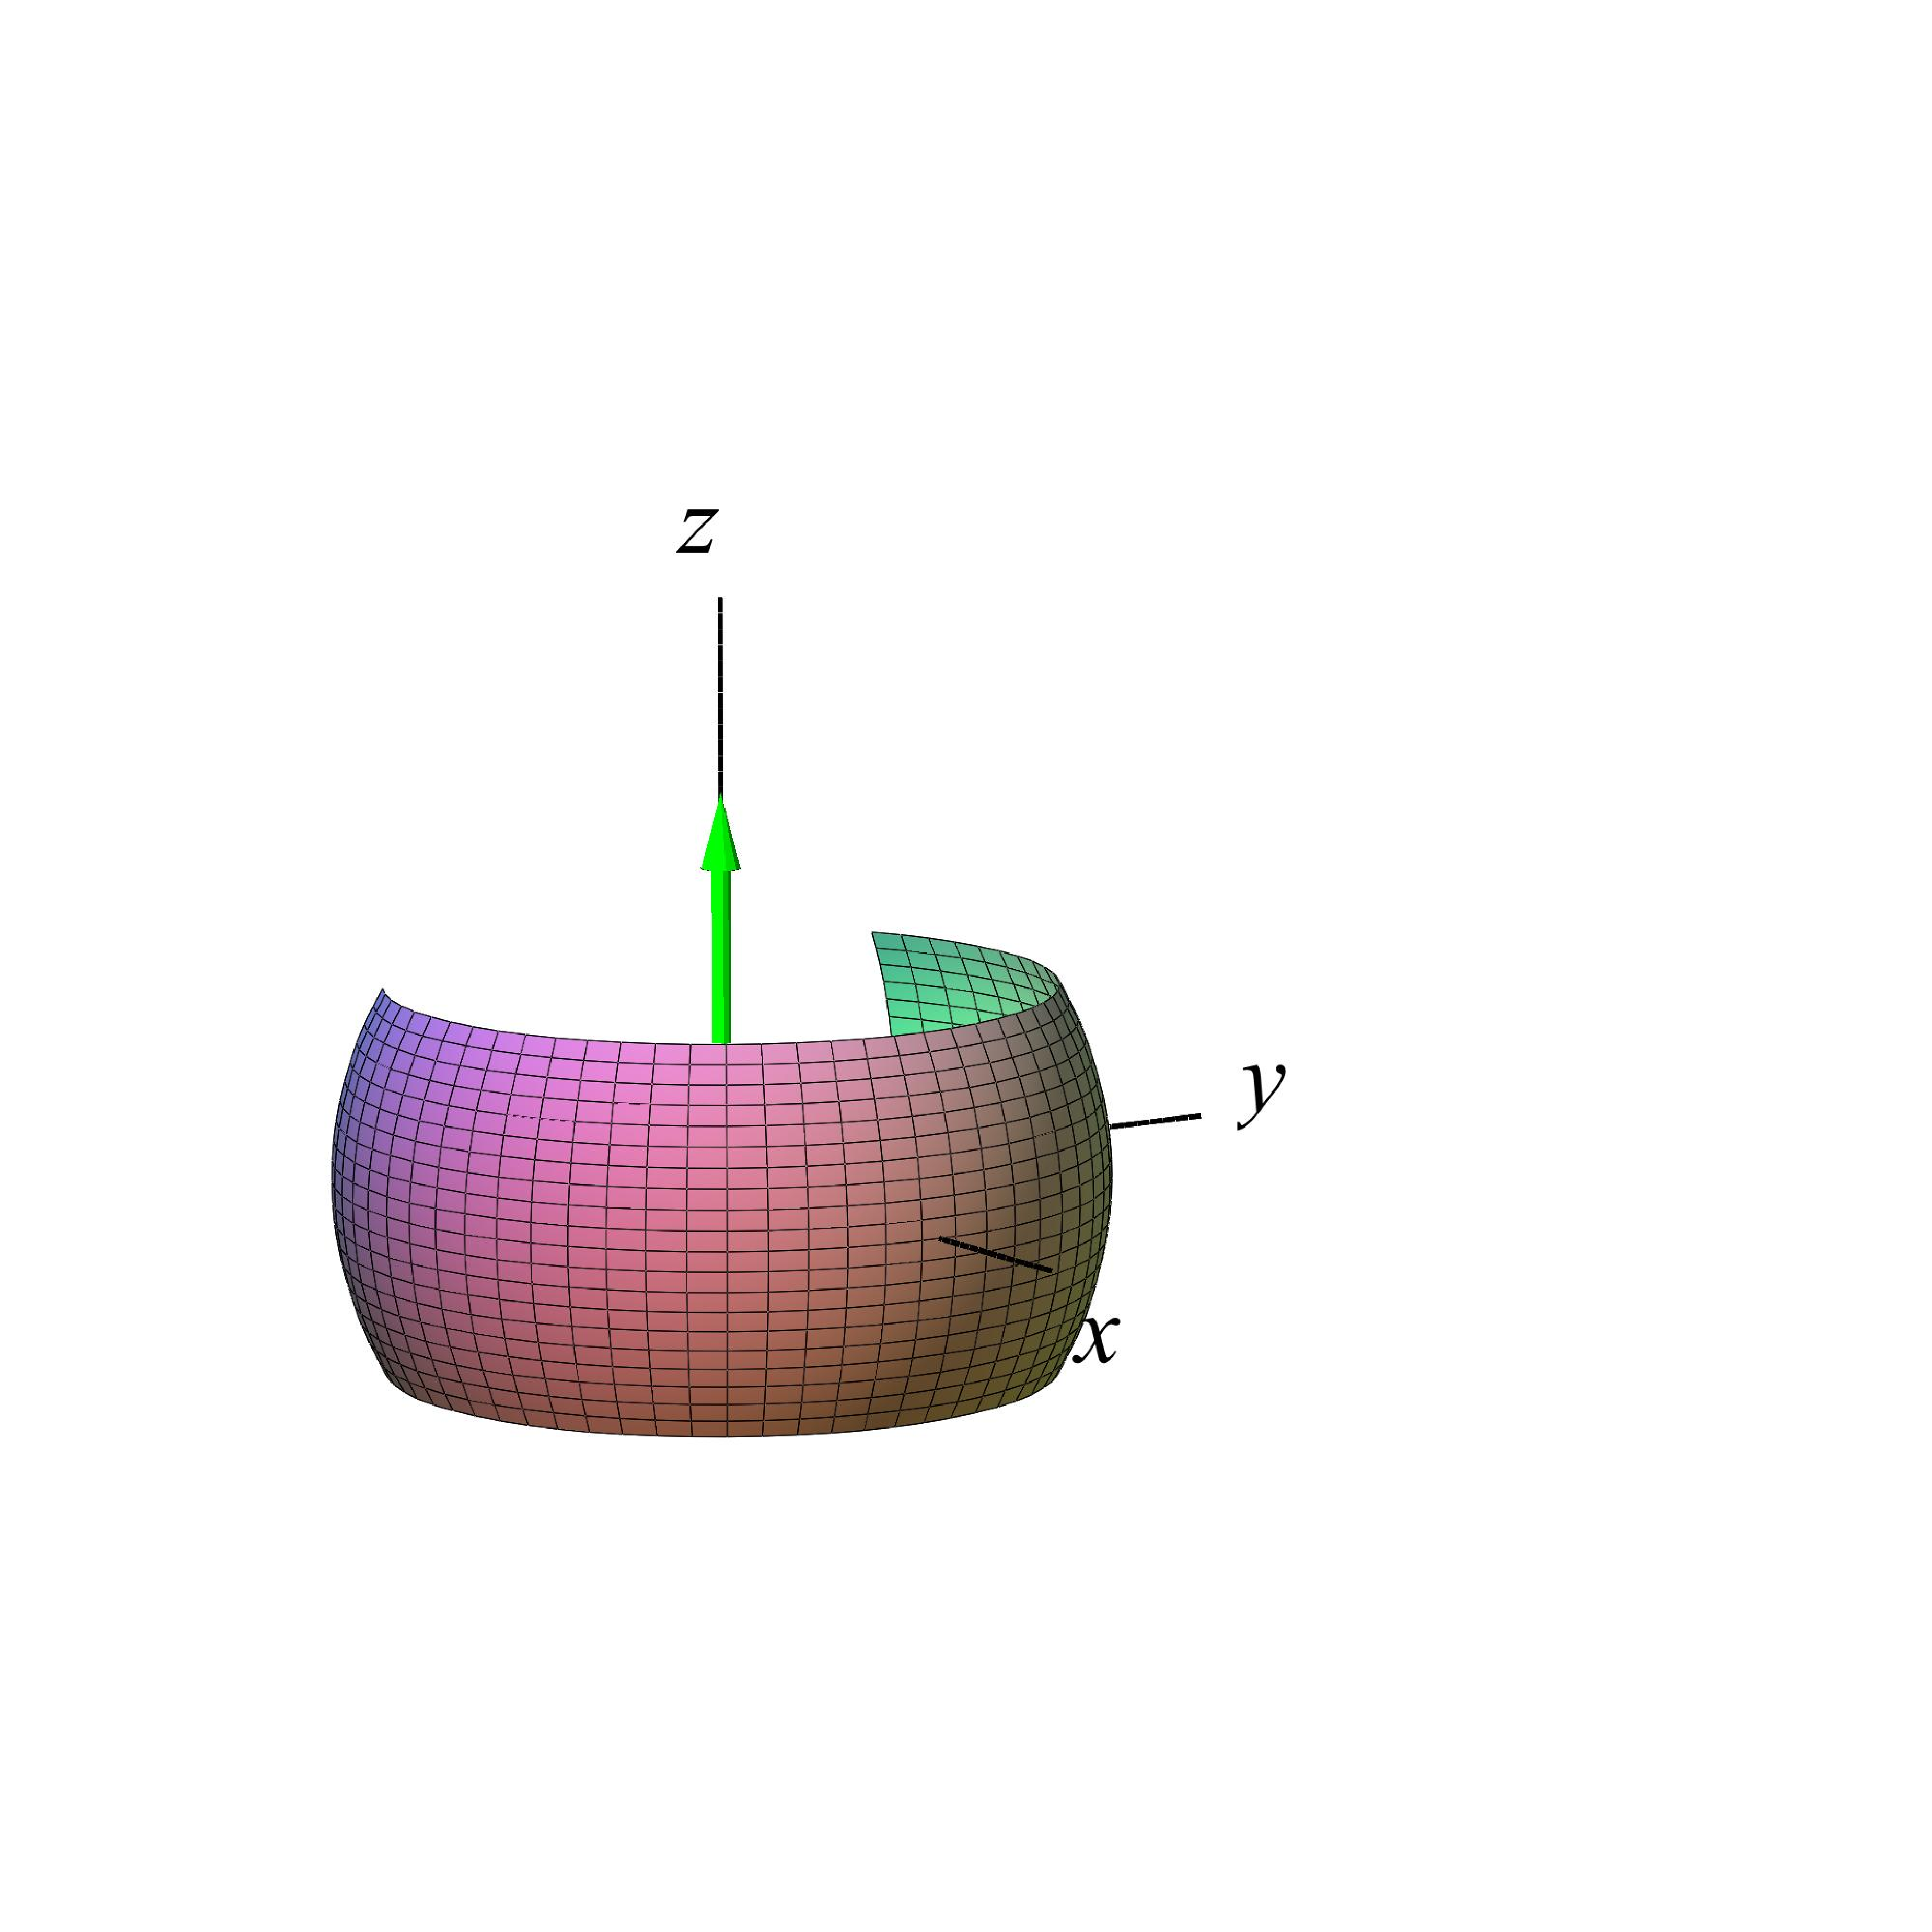
\includegraphics[height=50mm]{FIGS/plotKug2}}
\begin{center}
\caption{\small{Enheds-kuglefladen og en del af enheds-kuglefladen. Delen er konstrueret ved at indskrænke parameterdomænet til $(u,v) \in [\pi/3, 2\pi/3] \times [-2\pi/3, 2\pi/3]$. }} \label{figKugleflade}
\end{center}
\end{figure}

\begin{example}[Kugleflade-parametrisering] \label{exampKugleflade}
Hele kuglefladen med radius $R$ og centrum i $(0,0,0)$ kan parametriseres med 'geografiske' parametre således:
\begin{equation}
\mathcal{S}_{R} \quad : \quad \mathbf{r}(u,v) = (R\cdot\sin(u)\cdot \cos(v), R\cdot \sin(u)\cdot \sin(v), R\cdot \cos(u)) \quad ,
\end{equation}
hvor $u \in [0, \pi]$ og $v \in [-\pi , \pi ]$. \\

Jacobi-funktionen hørende til denne parametrisering fås af følgende beregninger:
\begin{equation}
\begin{aligned}
\mathbf{r}'_{u} &= R\cdot (\cos(u)\cdot\cos(v), \cos(u)\cdot \sin(v), -\sin(v)) \quad ,\\
\mathbf{r}'_{v} &= R\cdot (-\sin(u)\cdot \sin(v), \sin(u)\cdot \cos(v), 0) \quad ,\\
\Jac_{\mathbf{r}}(u,v) &= |\mathbf{r}'_{u} \times \mathbf{r}'_{v}| = R^{2} \cdot \sin(u) \quad.
\end{aligned}
\end{equation}
Denne parametrisering er hverken regulær overalt eller en-entydig i det givne parameter-område. Hvorfor ikke? Hvor og hvordan er der brud på regulariteten? Hvor og hvordan er der brud på en-entydigheden? Se afnit \tref{NUID35-secEllipsoideParam}{afsnit} i \tref{NUID35-tn20}{eNote}.
\end{example}


\begin{example}[Grafflader] \label{exampGraffladeParamRegul}
Enhver standard-parametrisering af en grafflade for en glat funktion $h(x,y)$ af to variable er en-entydig og regulær overalt.
Hvis vi ser på standard-parametriseringen
\begin{equation}
\mathbf{r}(u,v) = (u, v, h(u,v)) \quad , \, \, \,  u \in [a,b] \, \,
, \, \,  v \in [c,d]
\end{equation}
får vi
Jacobifunktionen ved følgende generelle beregning:
\begin{equation}
\begin{aligned}
\mathbf{r}'_{u}(u,v) &= (1, 0, h'_{u}(u,v)) \quad ,\\
\mathbf{r}'_{v}(u,v) &= (0, 1, h'_{v}(u,v)) \quad ,\\
\mathbf{r}'_{u}(u,v) \times \mathbf{r}'_{v}(u,v) &= (-h'_{u}(u,v), -h'_{v}(u,v), 1) \quad , \\
\Jac_{\mathbf{r}}(u,v) &= \sqrt{1 + (h'_{u}(u,v))^{2} + (h'_{v}(u,v))^{2}} = \sqrt{1 + |\bm{\nabla}h(u,v)|^{2}}  \quad , 
\end{aligned}
\end{equation}
som jo klart er positiv for alle $(u,v)$ i parameter-området.
\end{example}


\begin{definition}[Areal af flade] \label{defArealFlade}
{Arealet} af den parametriserede flade
$$F_{\bf r}: \quad {\bf r}(u,v) \, = \, \left(x(u,v), y(u,v),
z(u,v)\right) \quad , \, \, \,  u \in [a,b] \, \, , \, \,  v \in
[c,d] \quad
$$
defineres  som fladeintegralet af den konstante funktion $1$ over fladen:
\begin{equation} \label{eqFladeintegralAreal}
\Ar(F_{\bf r}) \, = \, \int_{F_{\bf r}} 1 \, d\mu \, = \,
\int_{c}^{d} \int_{a}^{b}  \Jac_{\bf r}(u,v)\,du \, dv \quad.
\end{equation}
\end{definition}



\begin{example}[Areal af graf-flader] \label{exampGraffladeAreal}
Arealet af graffladen for funktionen $h(x,y)$ over det rektangulære område $[a,b]\times [c, d]$ i $(x,y)$-planen er derfor:
\begin{equation}
\Ar(\widehat{\mathcal{F}}) = \int_{\widehat{\mathcal{F}}} 1 \, d\mu \, = \,
\int_{c}^{d} \int_{a}^{b}  \Jac_{\bf r}(u,v)\,du \, dv \quad,
\end{equation}
hvor
\begin{equation}
\begin{aligned}
\widehat{\mathcal{F}} = F_{\mathbf{r}}\quad : \quad \mathbf{r}(u,v) &= (u, v, h(u,v)) \quad , \quad   u \in [a,b] \, \, , \, \,  v \in
[c,d]  \quad , \\
\Jac_{\mathbf{r}}(u,v) &= \sqrt{1 + |\mathbf{\nabla}h(u,v)|^{2}}
\end{aligned}
\end{equation}
sådan at
\begin{equation}
\Ar(\widehat{\mathcal{F}}) = \int_{c}^{d} \int_{a}^{b} \sqrt{1 + |\mathbf{\nabla}h(u,v)|^{2}}\,du \, dv \quad.
\end{equation}
\end{example}



\begin{exercise} \label{exercRektangfareal}
Bestem arealet af den del af graffladen for funktionen $h(x,y) = x+y-1$ som ligger over kvadratet $(x,y) \in [0,1]\times [0,1]$ i $(x,y)$-planen. Bemærk, at denne del af graffladen er et plant parallelogram. Brug dels dobbelt-integration som i eksempel \ref{exampGraffladeAreal} og dels den klassiske arealbestemmelse ved hjælp af grundlinje og højde.
\end{exercise}


\begin{figure}[ht]
\centerline{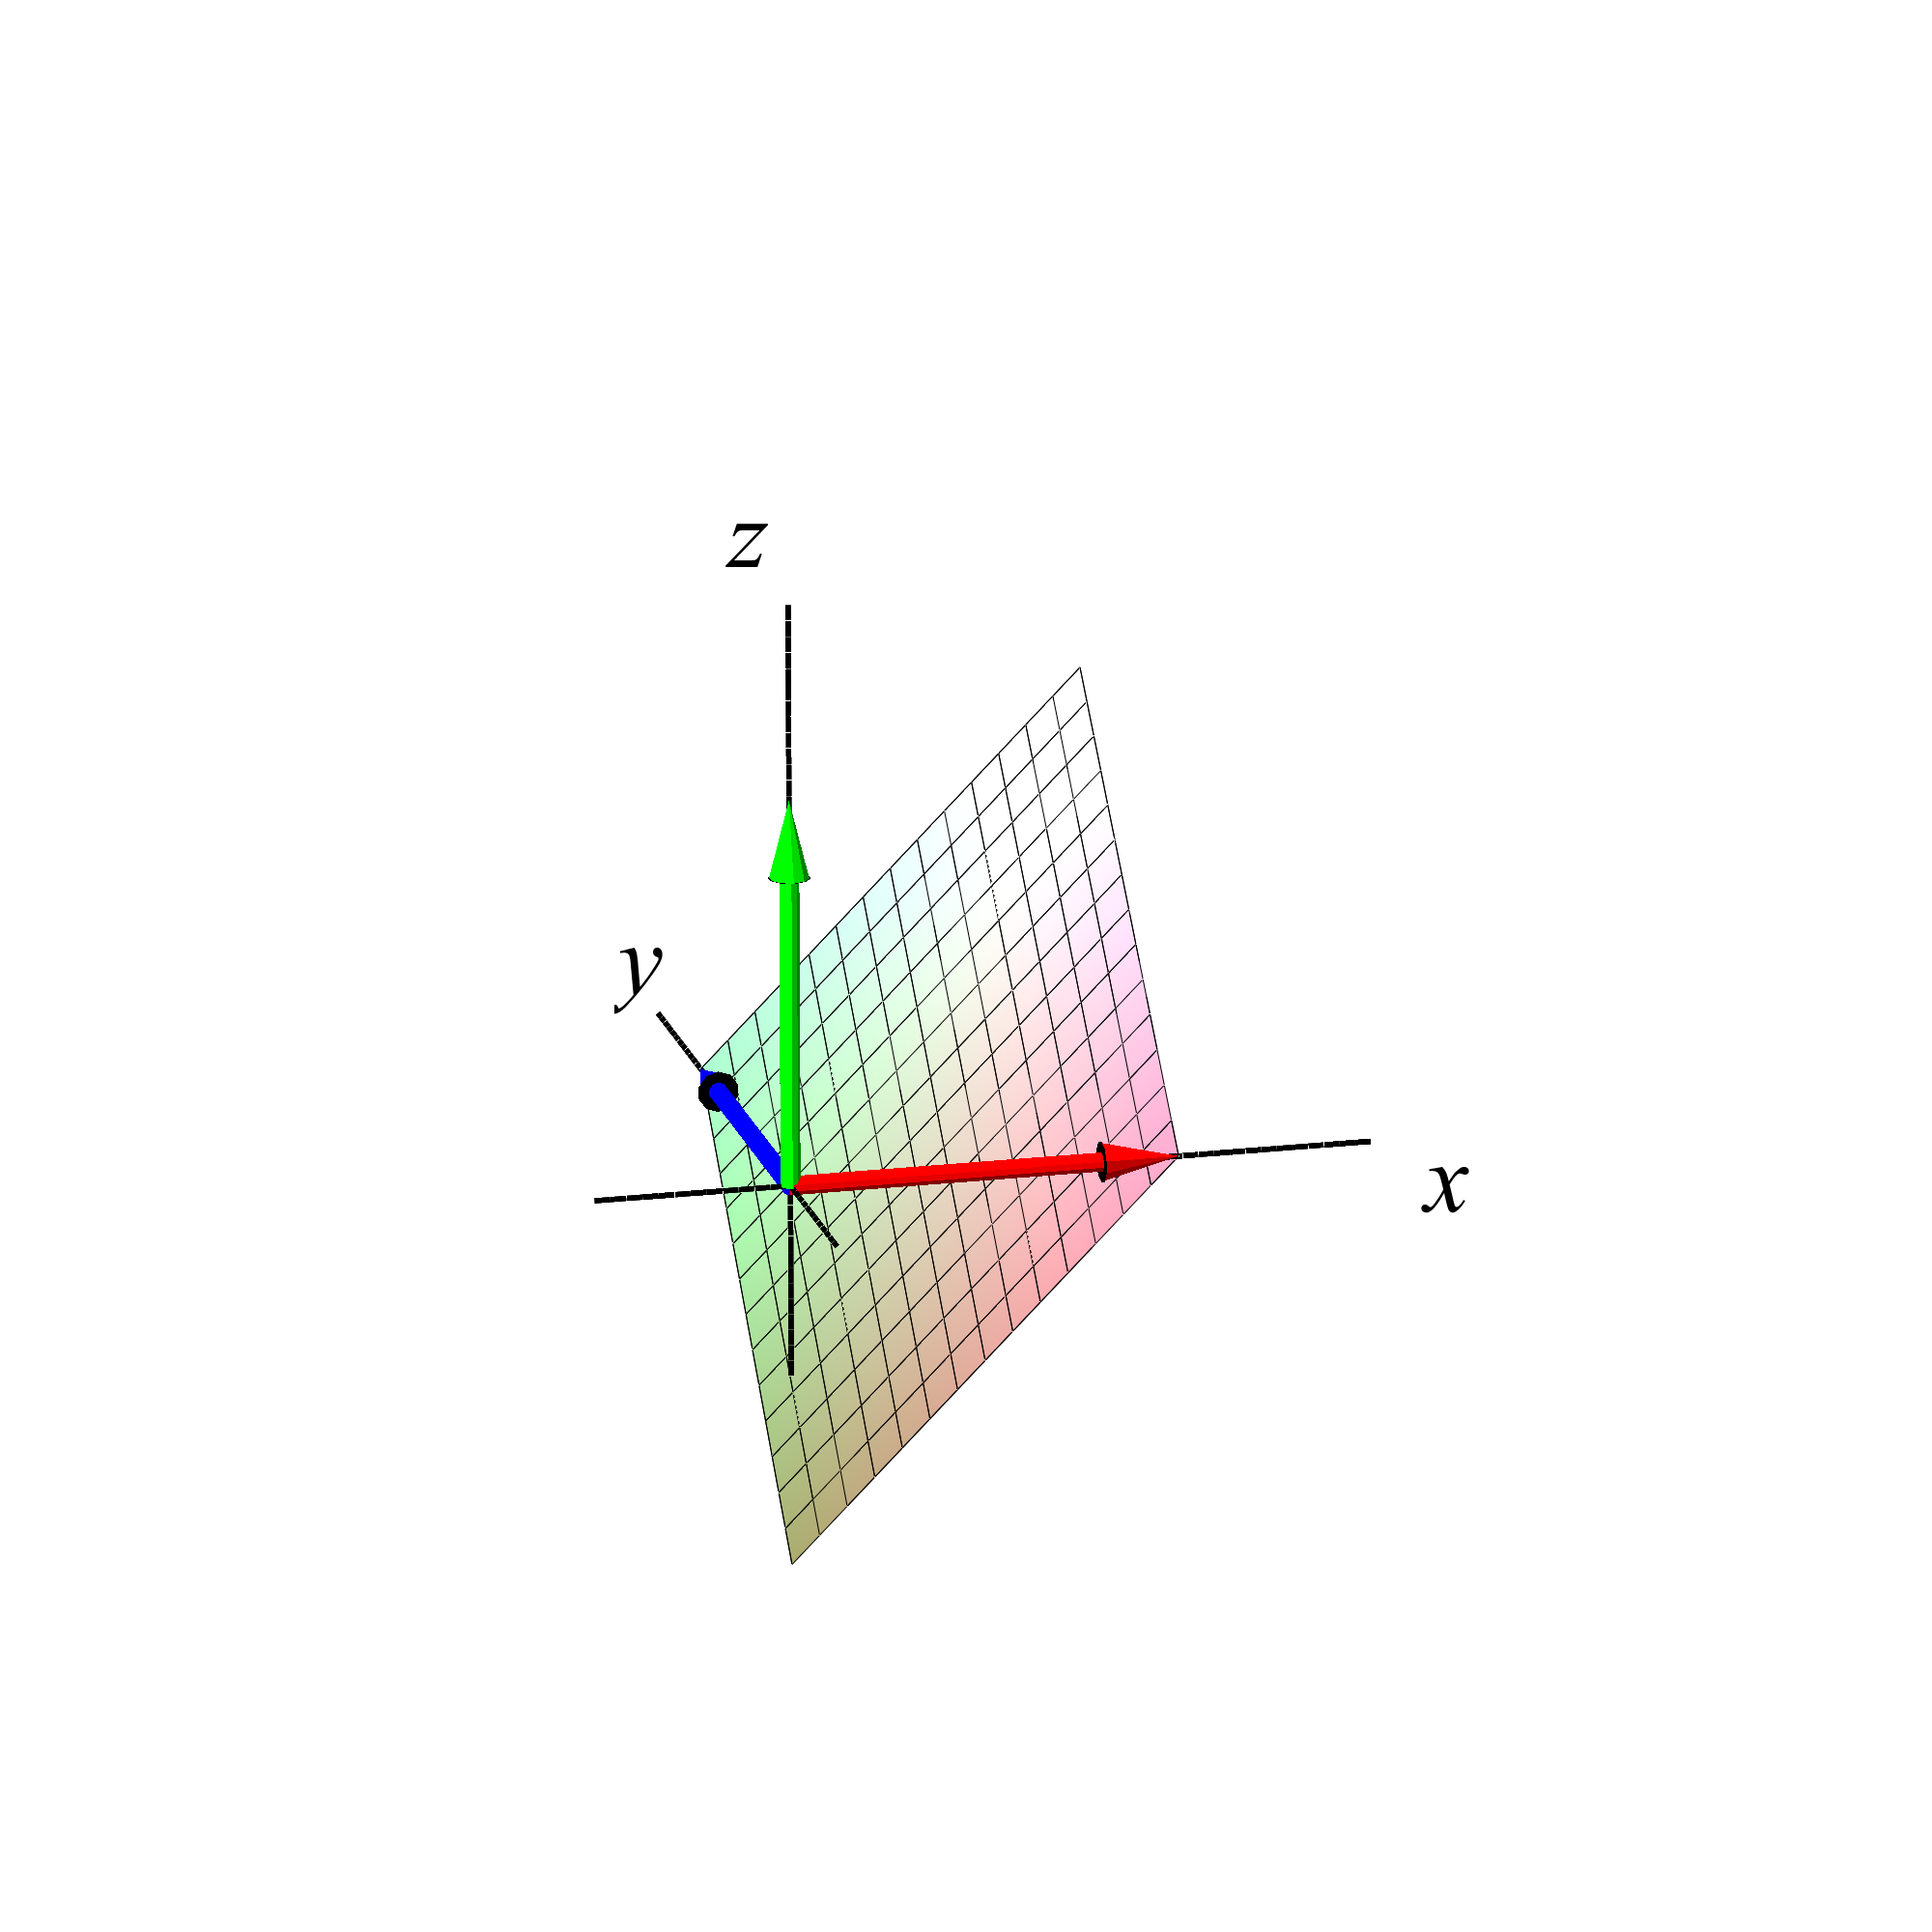
\includegraphics[height=75mm]{FIGS/plotGrafFlat1} \qquad \qquad 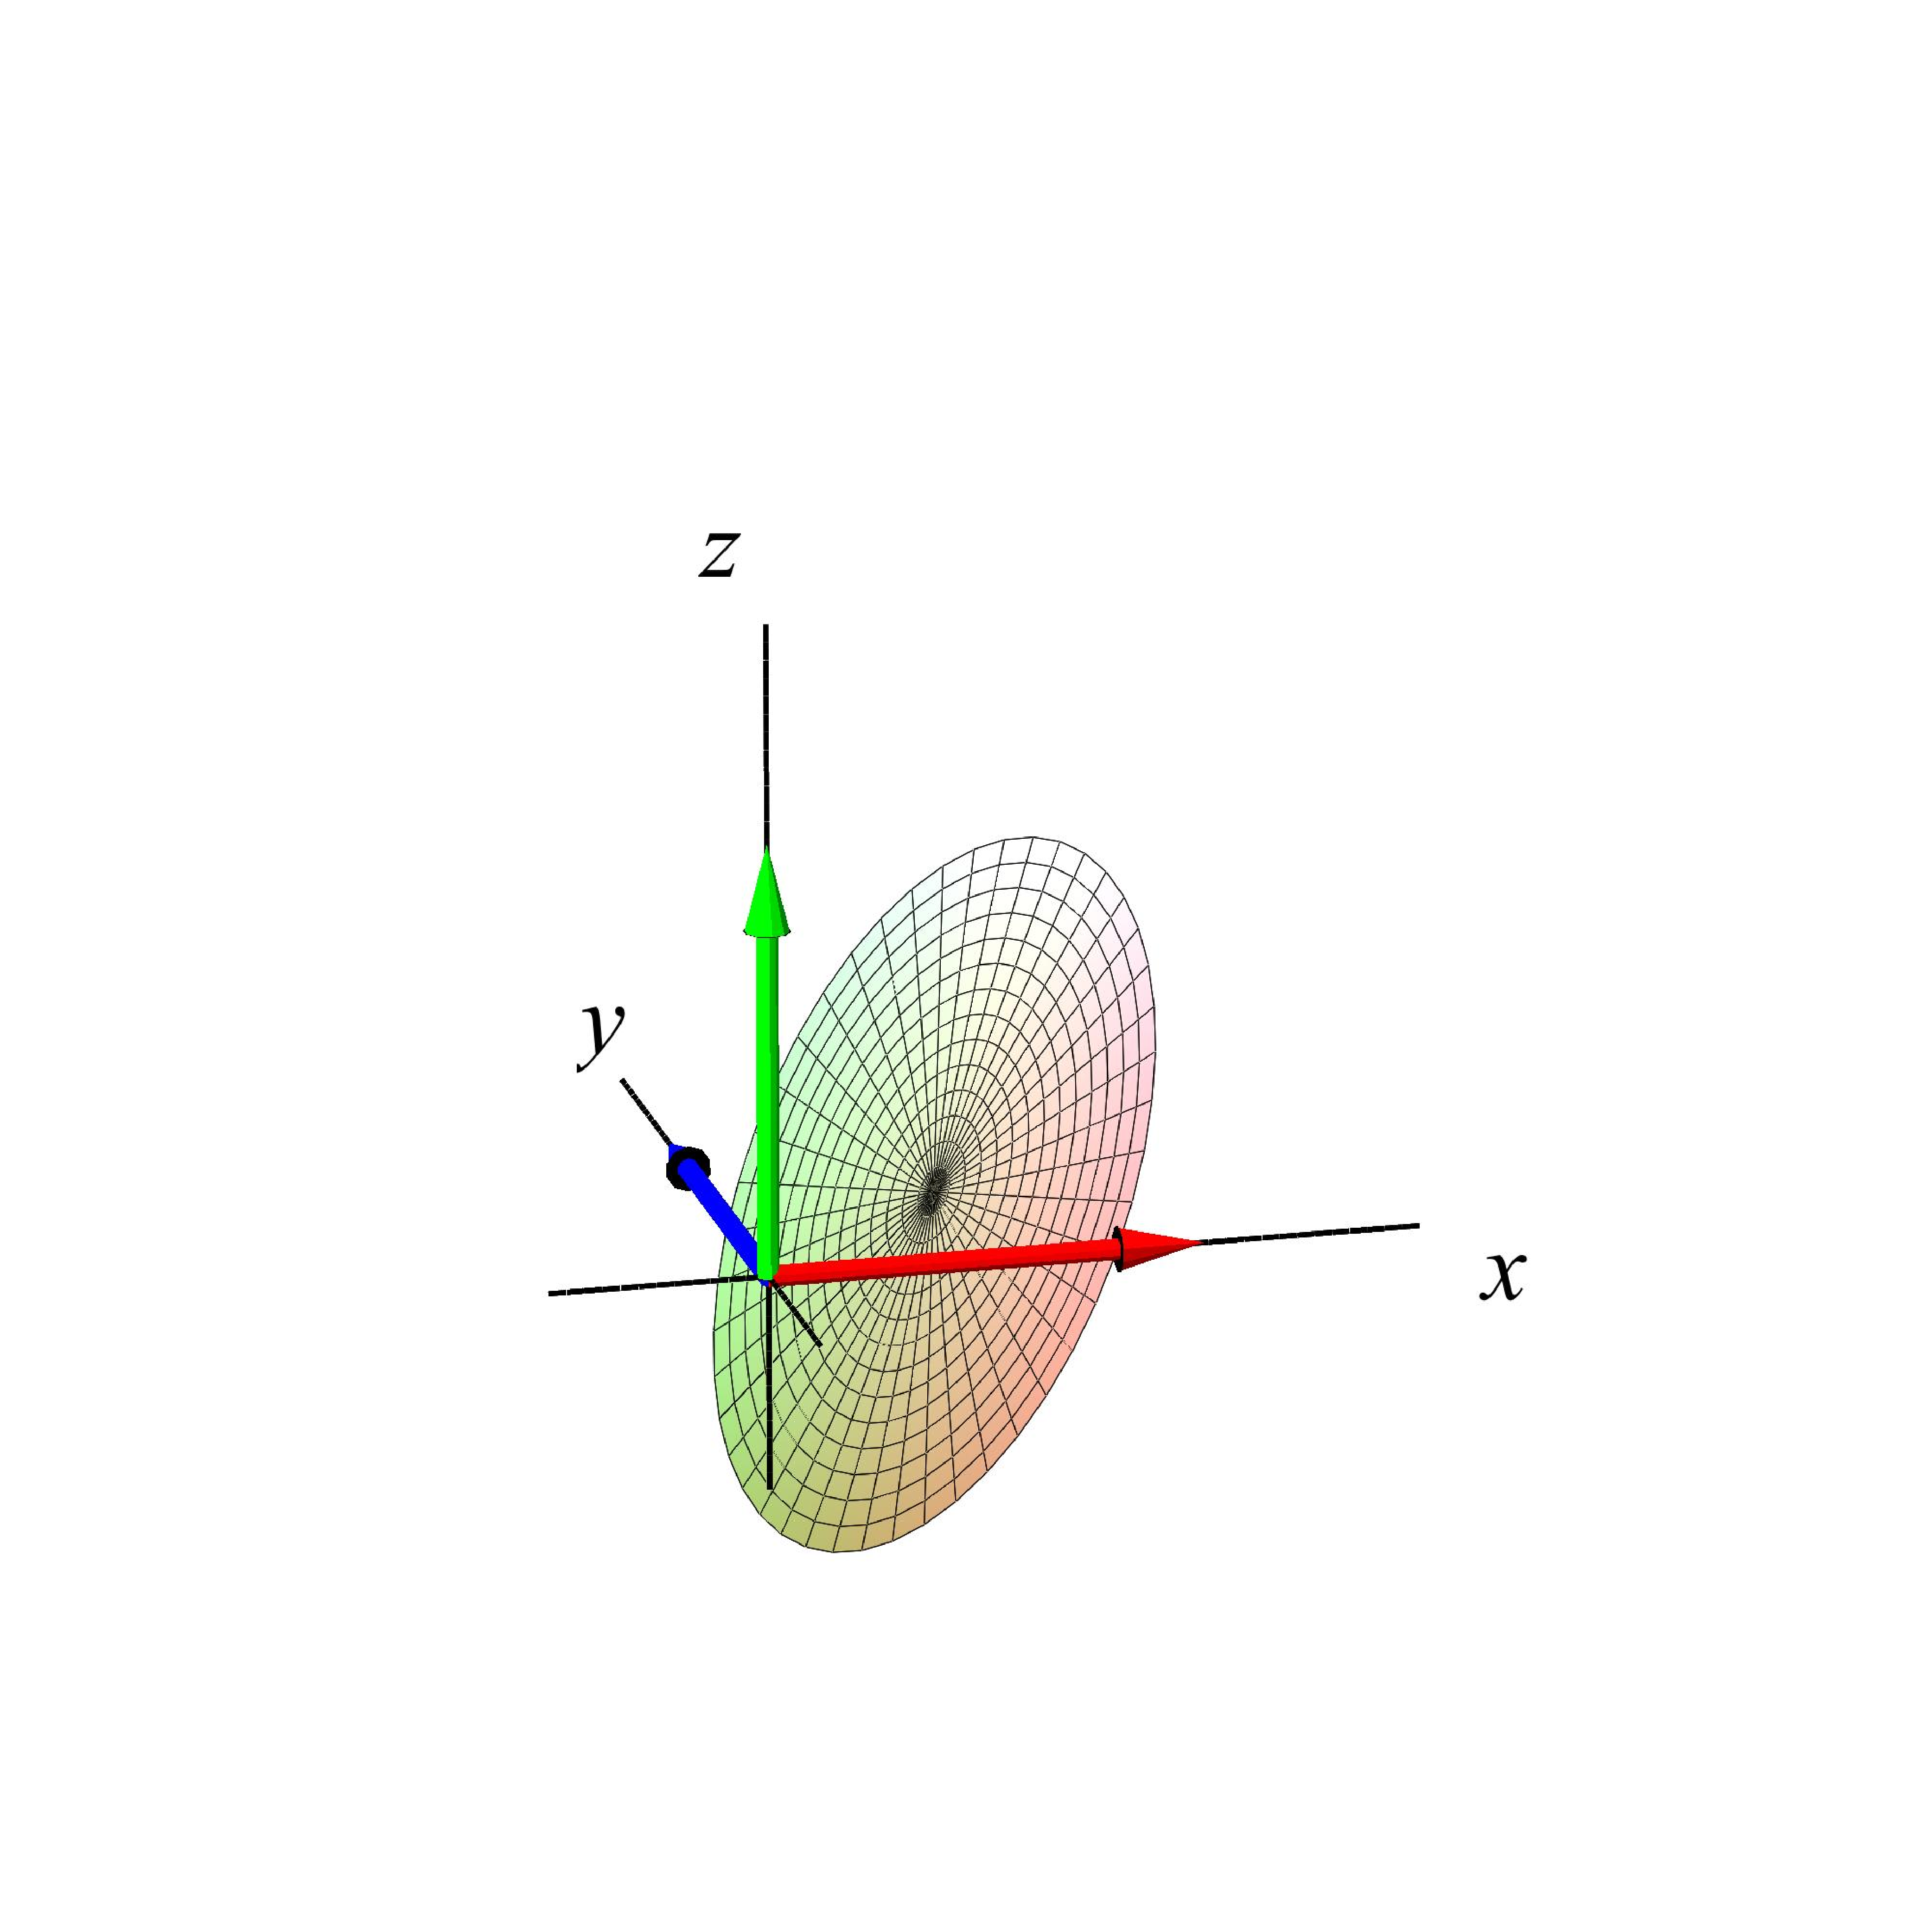
\includegraphics[height=75mm]{FIGS/plotGrafFlat2}}
\begin{center}
\caption{\small{Dele af en plan grafflade.}} \label{figGrafFlat}
\end{center}
\end{figure}


\begin{exercise} \label{exercCirkulfareal}
Bestem arealet af den del af graffladen for funktionen $h(x,y) = x+y-1 $ som ligger over den cirkelskive i $(x,y)$-planen som har radius $1/2$ og centrum i $(1/2, 1/2)$. Bemærk, at denne del af graffladen er et plant område, som er afgrænset af en ellipse.
\end{exercise}


\begin{exercise} \label{exercRektangUVareal}
Bestem arealet af den del af graf-fladen for funktionen $h(x,y) = x\cdot y$ som ligger over kvad\-ra\-tet $(x,y) \in [-1,1]\times [-1,1]$ i $(x,y)$-planen.
\end{exercise}

\begin{example}[Areal af kugleflade] \label{exampArealKugleflade}
En del af en kugleflade med radius $R$ og centrum i $(0,0,0)$ er parametriseret således:
\begin{equation}
\widehat{\mathcal{S}} \quad : \quad \widehat{\mathbf{r}}(u,v) = (R \cdot \sin(u)\cdot \cos(v), R \cdot \sin(u)\cdot \cos(v), R \cdot \cos(u)) \quad ,
\end{equation}
hvor $u \in [a, b] \subset [0, \pi]$ og $v \in [c , d ] \subset [-\pi, \pi]$. \\

Arealet af den del af kuglefladen er så, idet $\Jac_{\widehat{\mathbf{r}}}(u,v) = R^{2}\cdot \sin(u)$:
\begin{equation}
\begin{aligned}
\Ar(\widehat{\mathcal{S}}) &= \int_{c}^{d} \int_{a}^{b} R^{2} \cdot \sin(u) \,du \, dv \\
&= R^{2}\cdot (d-c)\cdot\left[-\cos(u) \right]_{u=a}^{u=b} \\
&= R^{2} \cdot (d-c)\cdot(\cos(a) - \cos(b)) \quad . \\
\end{aligned}
\end{equation}
Specielt får vi derfor også arealet af hele kuglefladen med $a=0$, $b=\pi$, $c=-\pi$, og $d=\pi$:
\begin{equation}
\Ar(\mathcal{S}_{R}) = 4\pi\cdot R^{2} \quad.
\end{equation}
\end{example}


\subsection{Motivering af fladeintegralet}\label{subsecMotivFlade}
Hvis vi  -- i stil med motiveringen af kurveintegralet --  deler {\em begge}
intervallerne $[a, b]$ og
 $[c, d]$ i henholdsvis $n$ og $m$
lige store dele, så har hvert $u$-delinterval længden $\delta_{u} \,
= \, (b-a)/n$ og hvert $v$-delinterval har længden $\delta_{v} \, =
\, (d-c)/m$. Tilsvarende bliver delepunkternes koordinater i $(u,
v)$-parameterområdet (som jo er rektanglet $[a,b]\times[c,d]$ i
$\mathbb{R}^{2}\,$) - jvf. afsnittet om dobbelt-integralsummer i \tref{NUID36-tn21}{eNote}:

\begin{equation}
\begin{aligned}
(u_{1}, v_{1}) \, &= \, (a, c), \\
(u_{1}, v_{j}) \, &= \, (a, c + (j-1)\delta_{v}), \\
(u_{i}, v_{1}) \, &= \, (a + (i-1)\delta_{u}, c), \\
(u_{i}, v_{j}) \, &= \, (a + (i-1)\delta_{u}, c + (j-1)\delta_{v}), \\
 &.... \\
(b, d) \, &= \, (a + n\delta_{u}, c + m\delta_{v}) \quad .
\end{aligned}
\end{equation}

Med hvert af disse faste punkter $(u_{i}, v_{j})$ som udviklingspunkt kan vi
betragte Taylor's grænseformel for hver af de 3 koordinat-funktioner for $\,{\bf r}(u,
v) \, = \, \left(x(u,v), y(u,v), z(u,v)\right)\, $ til første orden med tilhørende epsilon-funktioner:
\begin{equation} \label{eqTaylor2}
\begin{aligned}
{\bf r}(u, v) \, = \, {\bf r}(& u_{i}, v_{j}) \\
+ \, &{\bf r}'_{u}(u_{i}, v_{j})\cdot(u-u_{i}) \\
+ \, &{\bf r}'_{v}(u_{i}, v_{j})\cdot(v-v_{j}) \\
+ \, &\rho_{ij}\cdot {\bm{\varepsilon}}_{ij}(u-u_{i}, v-v_{i}) \quad
,
\end{aligned}
\end{equation}
hvor  $\, u\, \, \in\, \left[\, u_{i}\, , \,  u_{i} +
\delta_{u}\,\right]\, , \,\, v\, \, \in\, \left[\, v_{j}\, , \,
v_{j} + \delta_{v}\,\right] .$ Her betegner  $\, \rho_{ij} =
\sqrt{(u - u_{i})^{2} + (v - v_{j})^{2}}\, $ afstanden mellem det
variable punkt $\,(u\,, v)\,$ og det faste udviklingspunkt
$\,(u_{i}\,,v_{j})\,$ i parameterområdet. Der gælder her, at
$\,{\bm{\varepsilon}}_{ij}(u-u_{i}, v-v_{j}) \to (0, 0, 0)\, = \
{\bf{0}}\,$ for $\,(u-u_{i}, v-v_{j}) \to (0, 0)\,$ .


Hvert delrektangel $[u_{i}, u_{i}+\delta_{u}]\times[v_{j},
v_{j}+\delta_{v}]$ afbildes på flade-{\em stykket} ${\bf r}(u,v)$,
$u \in[u_{i}, u_{i}+\delta_{u}], v \in[v_{j}, v_{j}+\delta_{v}]$ og
dette fladestykke kan vi approksimere med den lineære del af
udtrykket i (\ref{eqTaylor2}), som fås ved at fjerne
${\bm{\varepsilon}}_{ij}$-bidraget fra højre side i
(\ref{eqTaylor2}):
\begin{equation}\label{eqApp2}
{\bf r}_{\app_{\,ij}}(u, v) \, = \, {\bf r}(u_{i}, v_{j}) + \, {\bf
r}'_{u}(u_{i}, v_{j})\cdot (u - u_{i}) + \, {\bf r}'_{v}(u_{i},
v_{j})\cdot (v - v_{j}) \quad ,
\end{equation}
hvor $u$ og $v$ stadig gennemløber del-intervallerne $\, u\, \,
\in\, \left[\, u_{i}\, , \,  u_{i} + \delta_{u}\,\right]\, , \,\,
v\, \, \in\, \left[\, v_{j}\, , \, v_{j} + \delta_{v}\,\right] .$


 Disse lineære approksimationer er parallelogrammer,
som udspændes af de to tangentvektorer ${\bf
r}'_{u}(u_{i}, v_{j})\cdot\delta_{u}$ og ${\bf
r}'_{v}(u_{i}, v_{j})\cdot \delta_{v}$. Se Figur
\ref{figKegle12} hvor de approksimerende
parallelogrammer er vist for en parametrisering
af en kegleflade.


\subsubsection{Areal}\label{subsubsecAreal}
Hvert enkelt af de ialt $n\,m$ approksimerende
parallelogrammer har et areal. Arealet af det
$(i, j)$'te parallelogram er længden af
krydsproduktet af de to vektorer, der udspænder
det pågældende parallelogram:

\begin{equation}
\Delta \Ar_{ij} \, = \,  | ({\bf r}'_{u}(u_{i}, v_{j})\cdot
\delta_{u})\times ({\bf r}'_{v}(u_{i}, v_{j})\cdot \delta_{v}) |  \,
= \, \Jac_{\bf r}(u_{i}, v_{j})\cdot \delta_{u}\delta_{v} \quad.
\end{equation}



\begin{exercise}
Bevis denne påstand: Arealet af et parallelogram
er længden af krydsproduktet af de to vektorer,
der udspænder parallelogrammet.
\end{exercise}


Summen af disse ialt $n\cdot m$ arealer er klart en god approksimation
til arealet af hele fladestykket, således at vi har
\begin{equation}
\Ar_{\app}(n,m)\, = \,   \sum_{j=1}^{m}\sum_{i=1}^{n} \Delta \Ar_{ij}
\, = \,  \sum_{j=1}^{m}\sum_{i=1}^{n} \Jac_{\bf r}(u_{i},
v_{j})\cdot \delta_{u} \delta_{v}  \quad.
\end{equation}
Da ovenstående sum er en dobbelt integralsum for den kontinuerte
funktion $\, \Jac_{\bf r}(u, v)\, $ over parameter-rektanglet $\,
[a, b]\times[c, d]\, $ får vi i grænsen, hvor $n$ og $m$ begge går
mod uendelig (jvf. \tref{NUID36-tn21}{eNote}):
\begin{equation}
\Ar_{\app}(n,m)\,  \to \, \Ar\, = \, \int_{c}^{d} \int_{a}^{b}
\Jac_{\bf r}(u, v) \,du \, dv \, = \, \int_{F_{\bf r}} 1 \, d\mu \, \quad \text{for} \quad n\, , \, m  \to
\infty \quad.
\end{equation}

Dette er begrundelsen for definitionen af arealet af en
parametriseret flade som angivet ovenfor, nemlig som
fladeintegralet af den konstante funktion $1$.



\begin{figure}[h]
\centerline{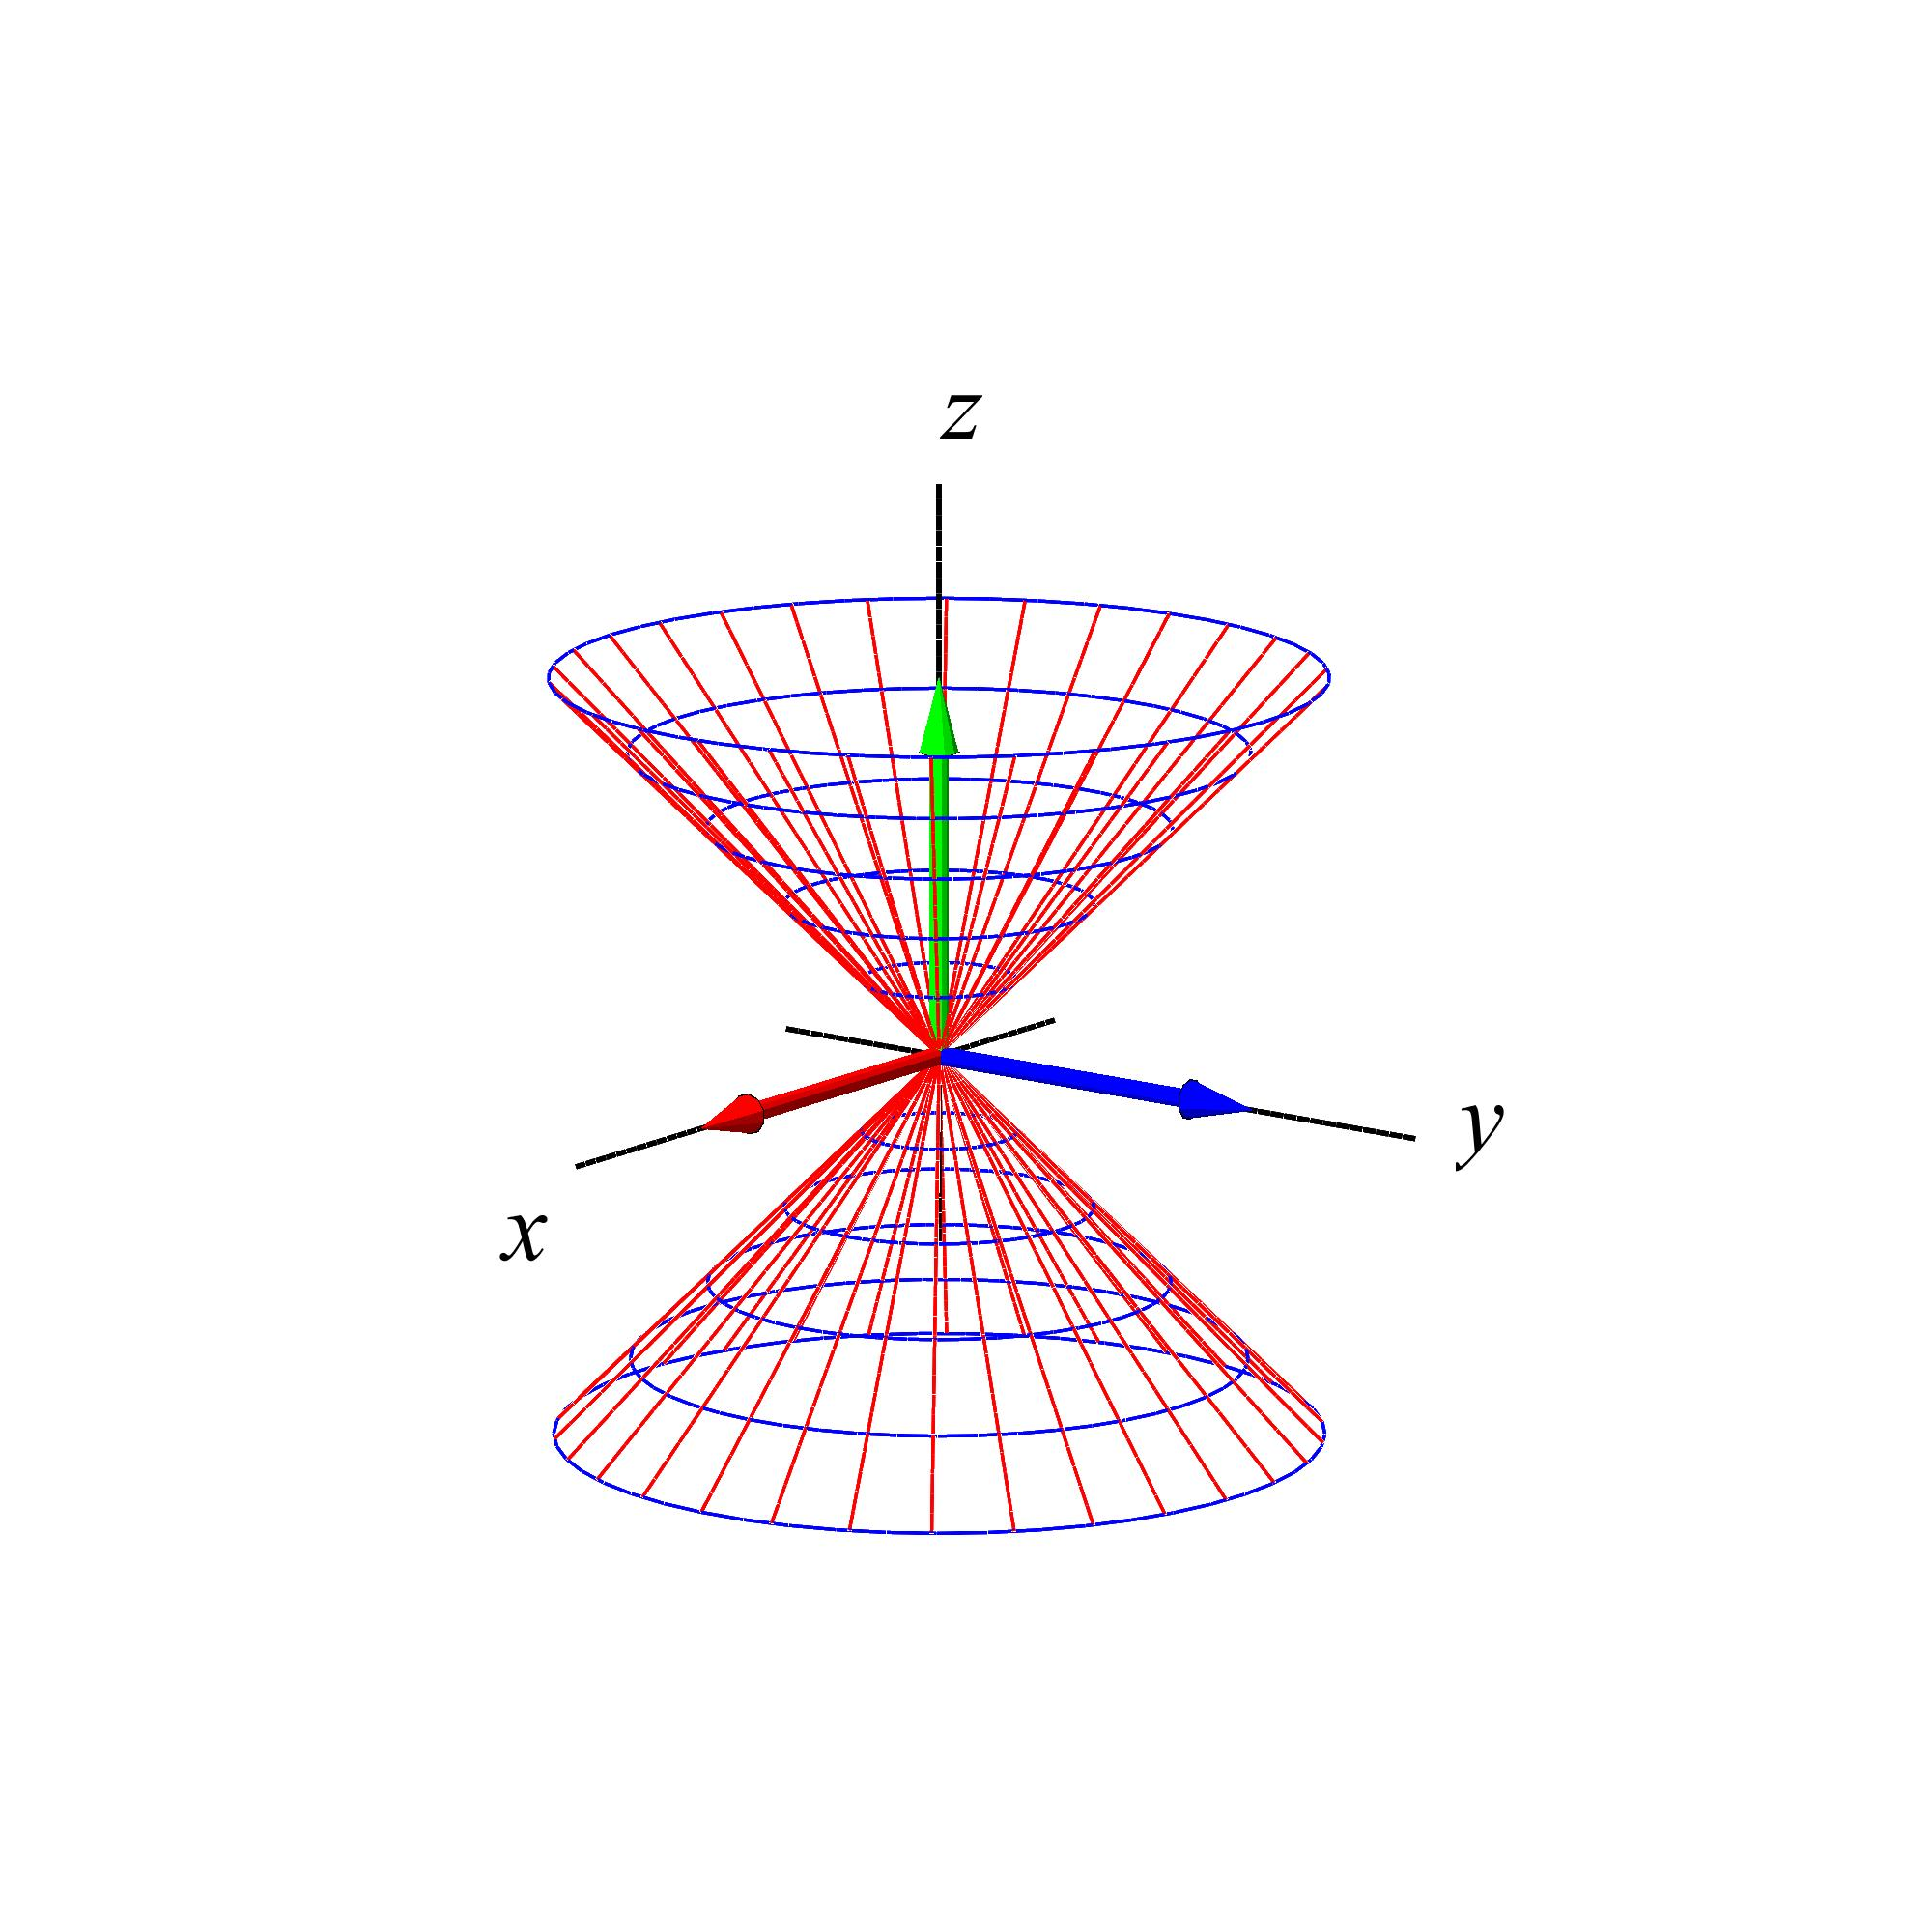
\includegraphics[height=60mm]{FIGS/plotKegle1}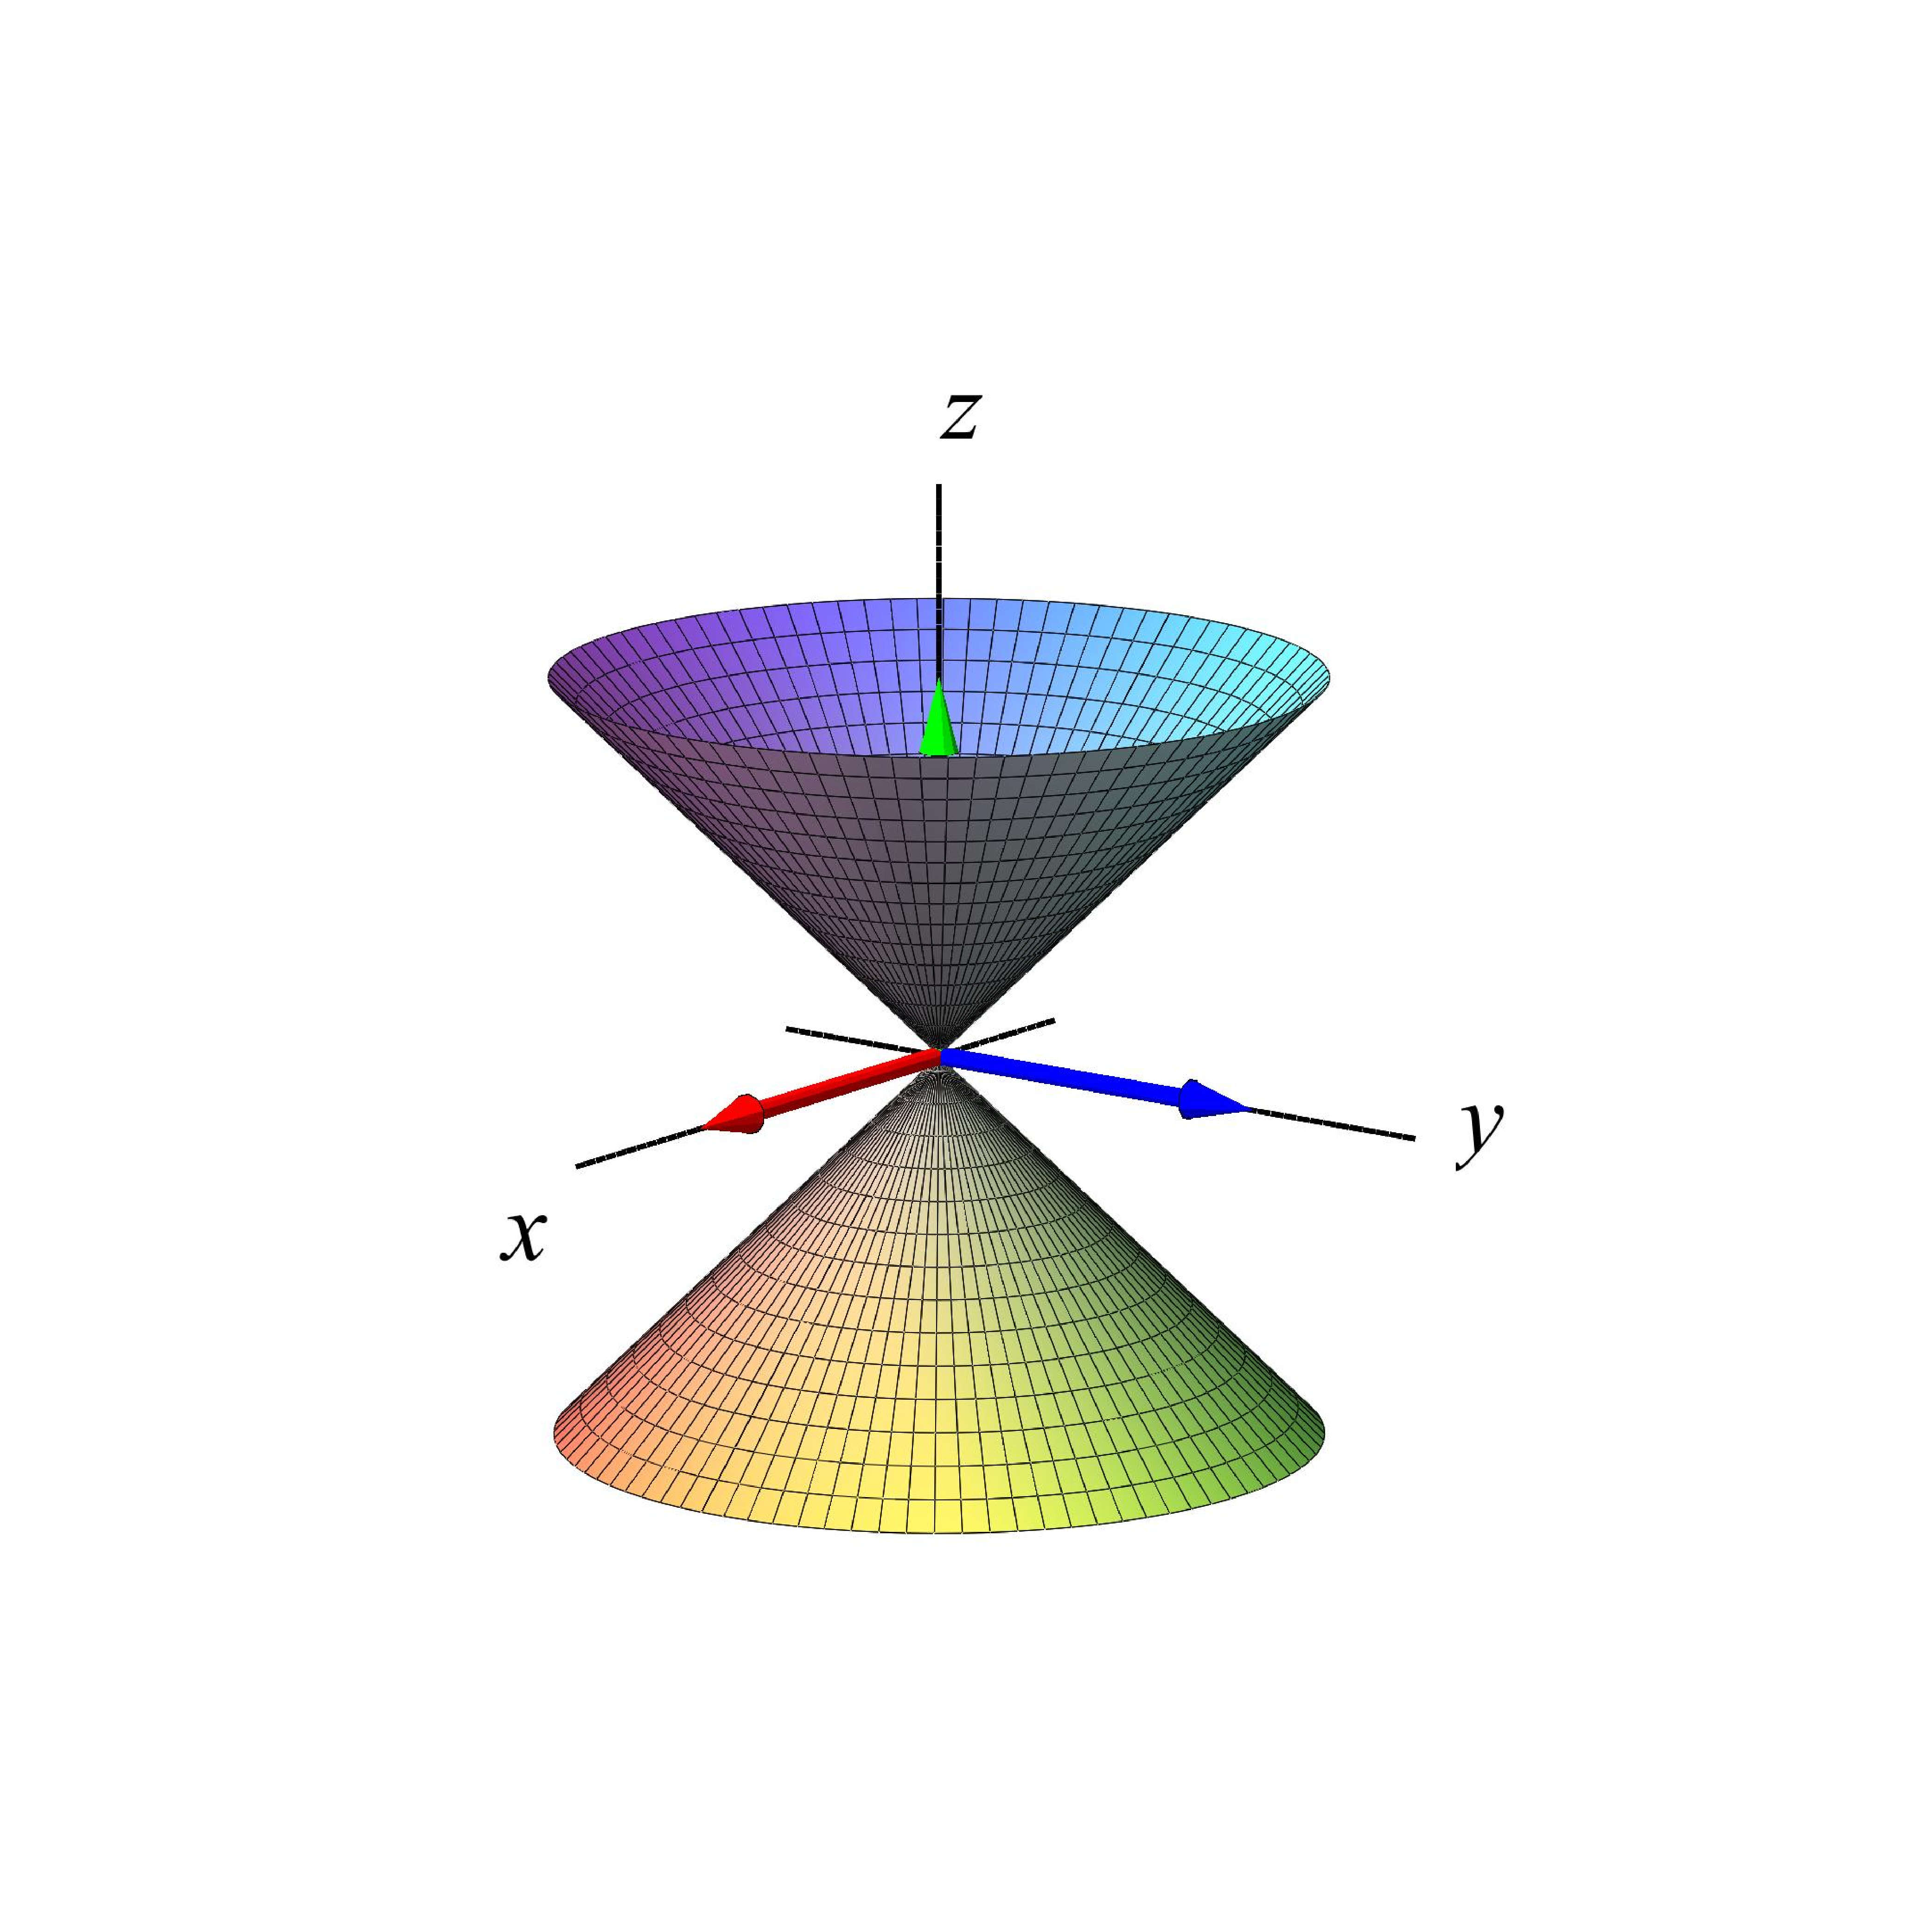
\includegraphics[height=60mm]{FIGS/plotKegle2}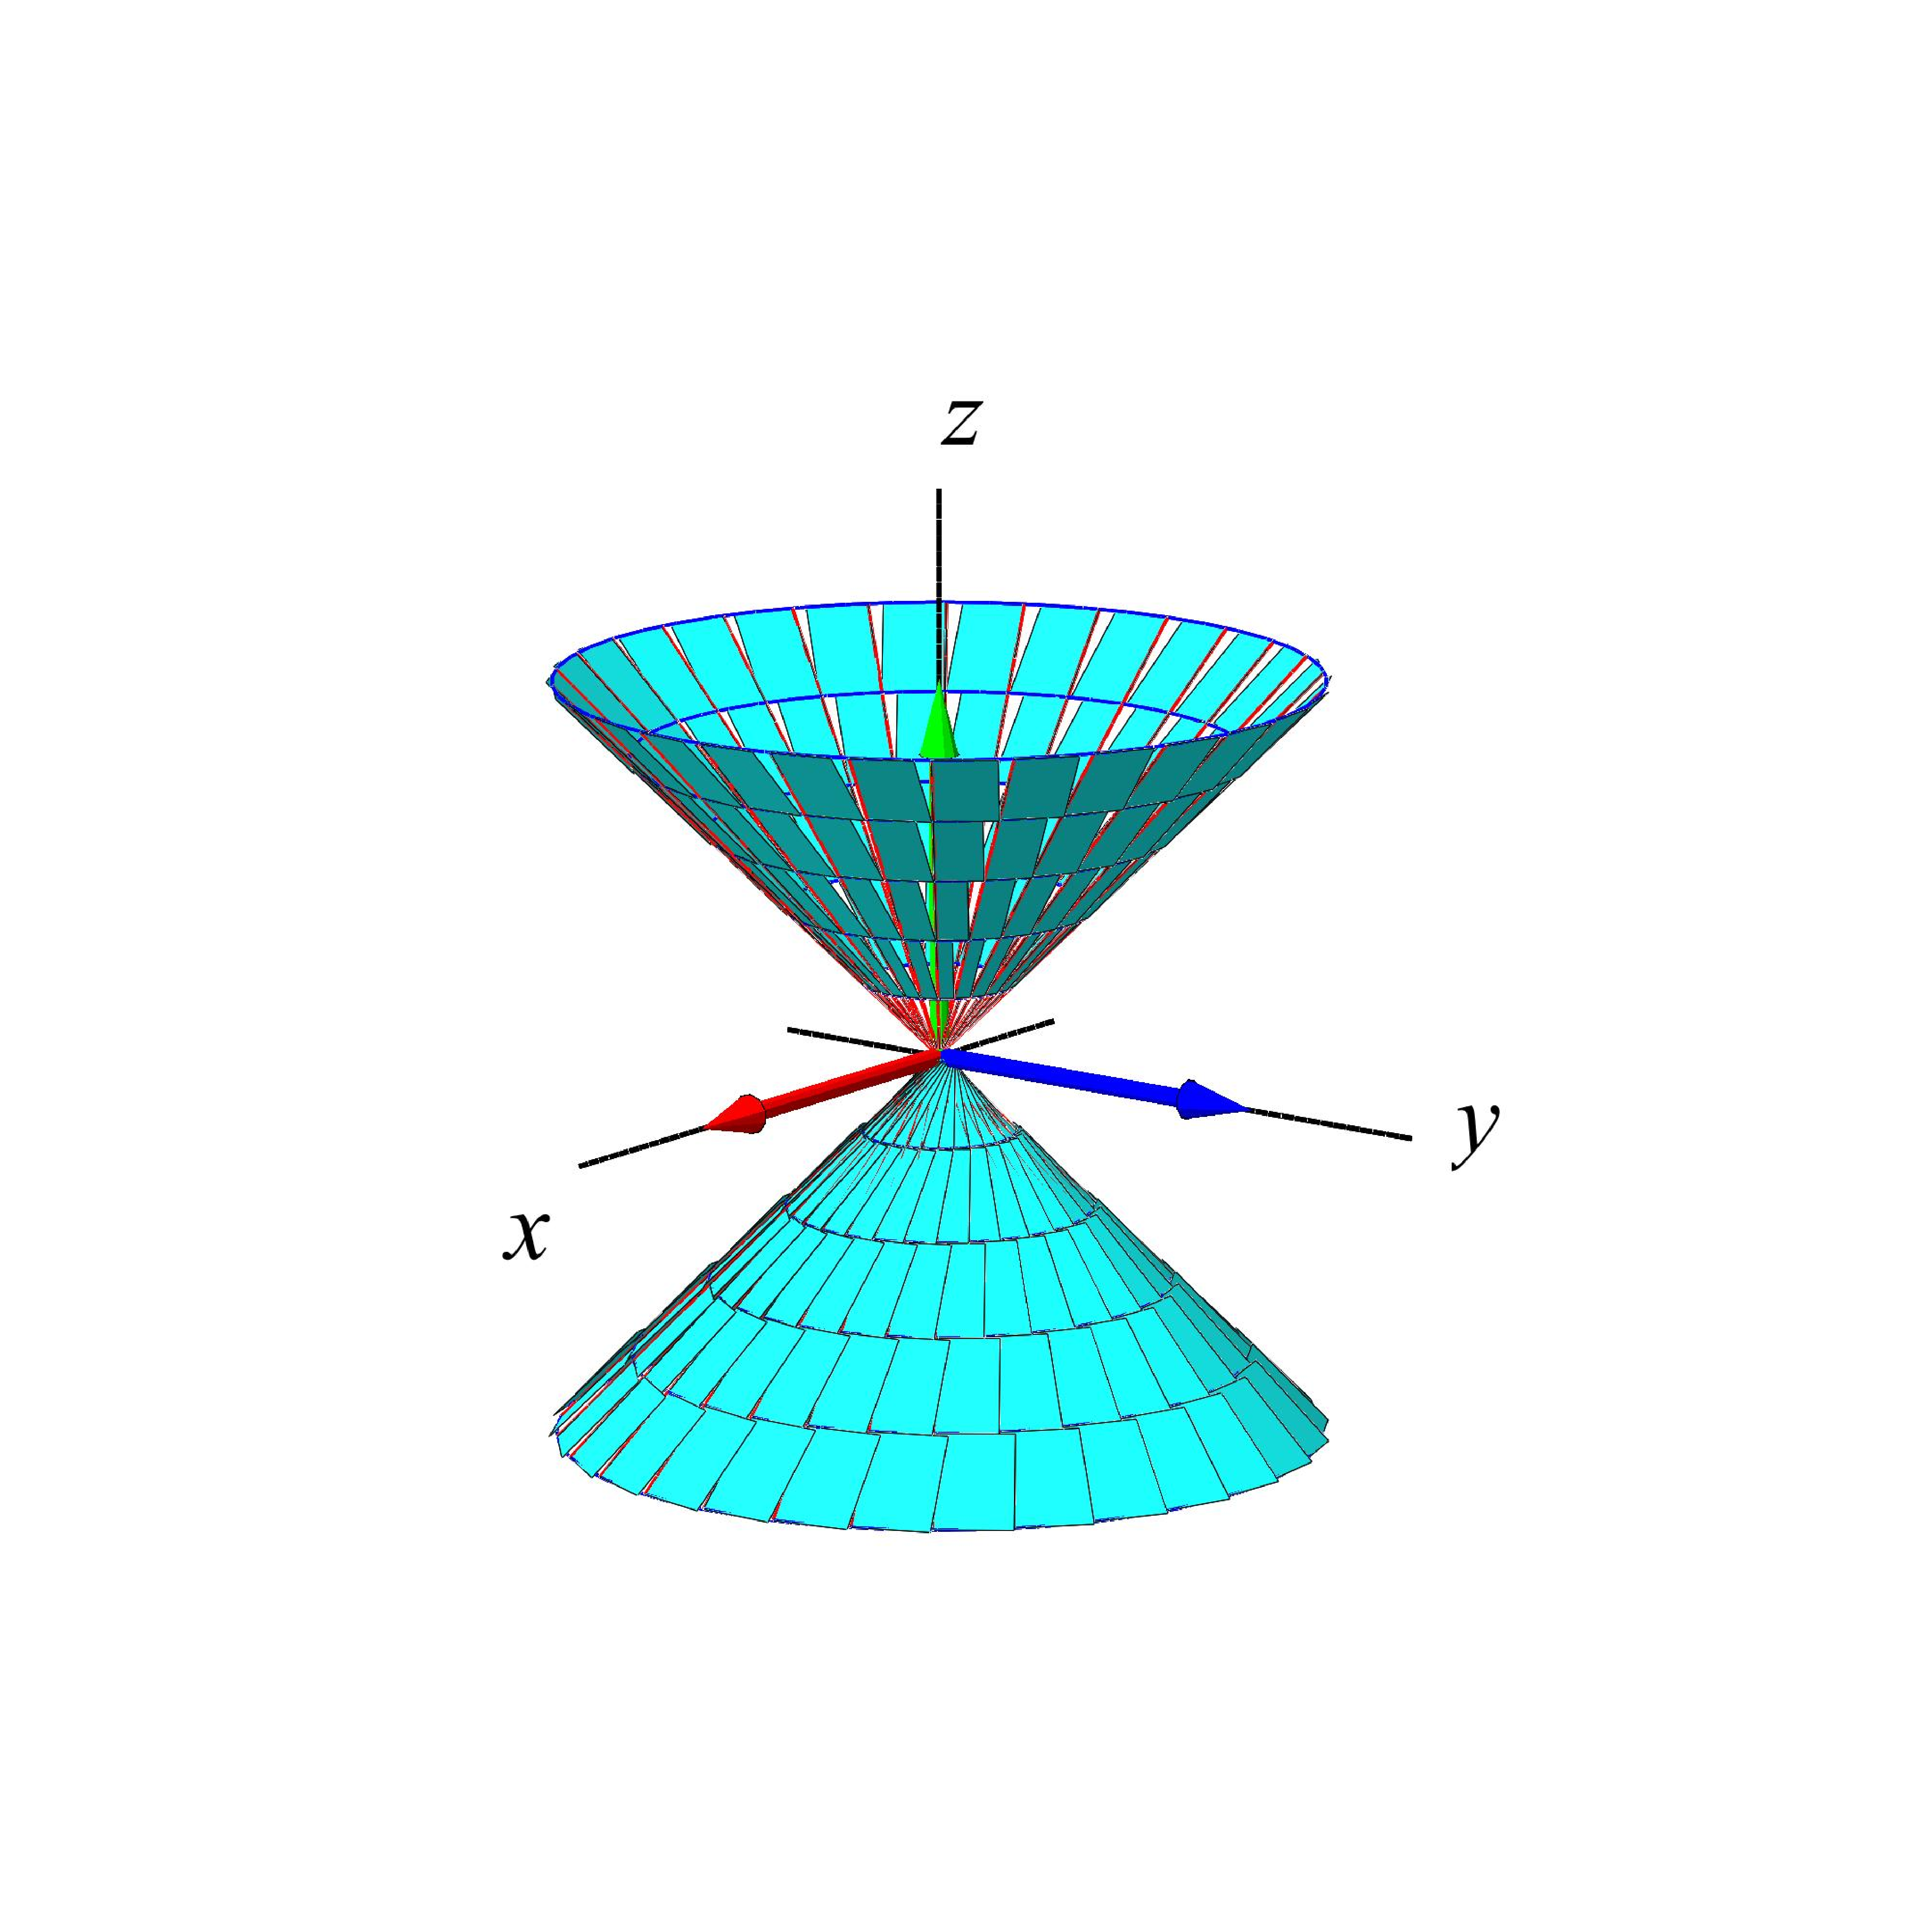
\includegraphics[height=60mm]{FIGS/plotKegle3} }
\begin{center}
\caption{\small{Kegle-fladen er givet ved
parameterfremstillingen ${\bf r}(u, v) \, = \,
(u\cos(v), u\sin(v), u) \,\,, \,\, u \in [-1, 1
]\,\, , \, \, v \in [-\pi, \pi]$. Et system af
koordinatkurver på fladen er vist til venstre og
de tilsvarende areal-approksimerende
parallelogrammer er vist til højre.}} \label{figKegle12}
\end{center}
\end{figure}


\begin{exercise}
Vis, at den givne parameterfremstilling i figur \ref{figKegle12}
hverken er regulær eller en-entydig i det givne parameterområde. Overvej, om der findes en
regulær parameterfremstilling for keglefladen.
\end{exercise}

\begin{exercise}
Hvorfor er de approksimerende parallelogrammer på
den øvre halvdel af keglefladen i figur
\ref{figKegle12} mindre end de tilsvarende
parallelogrammer (med samme afstand til
toppunktet) på den nedre halvdel?
\end{exercise}







\begin{figure}[h]
\centerline{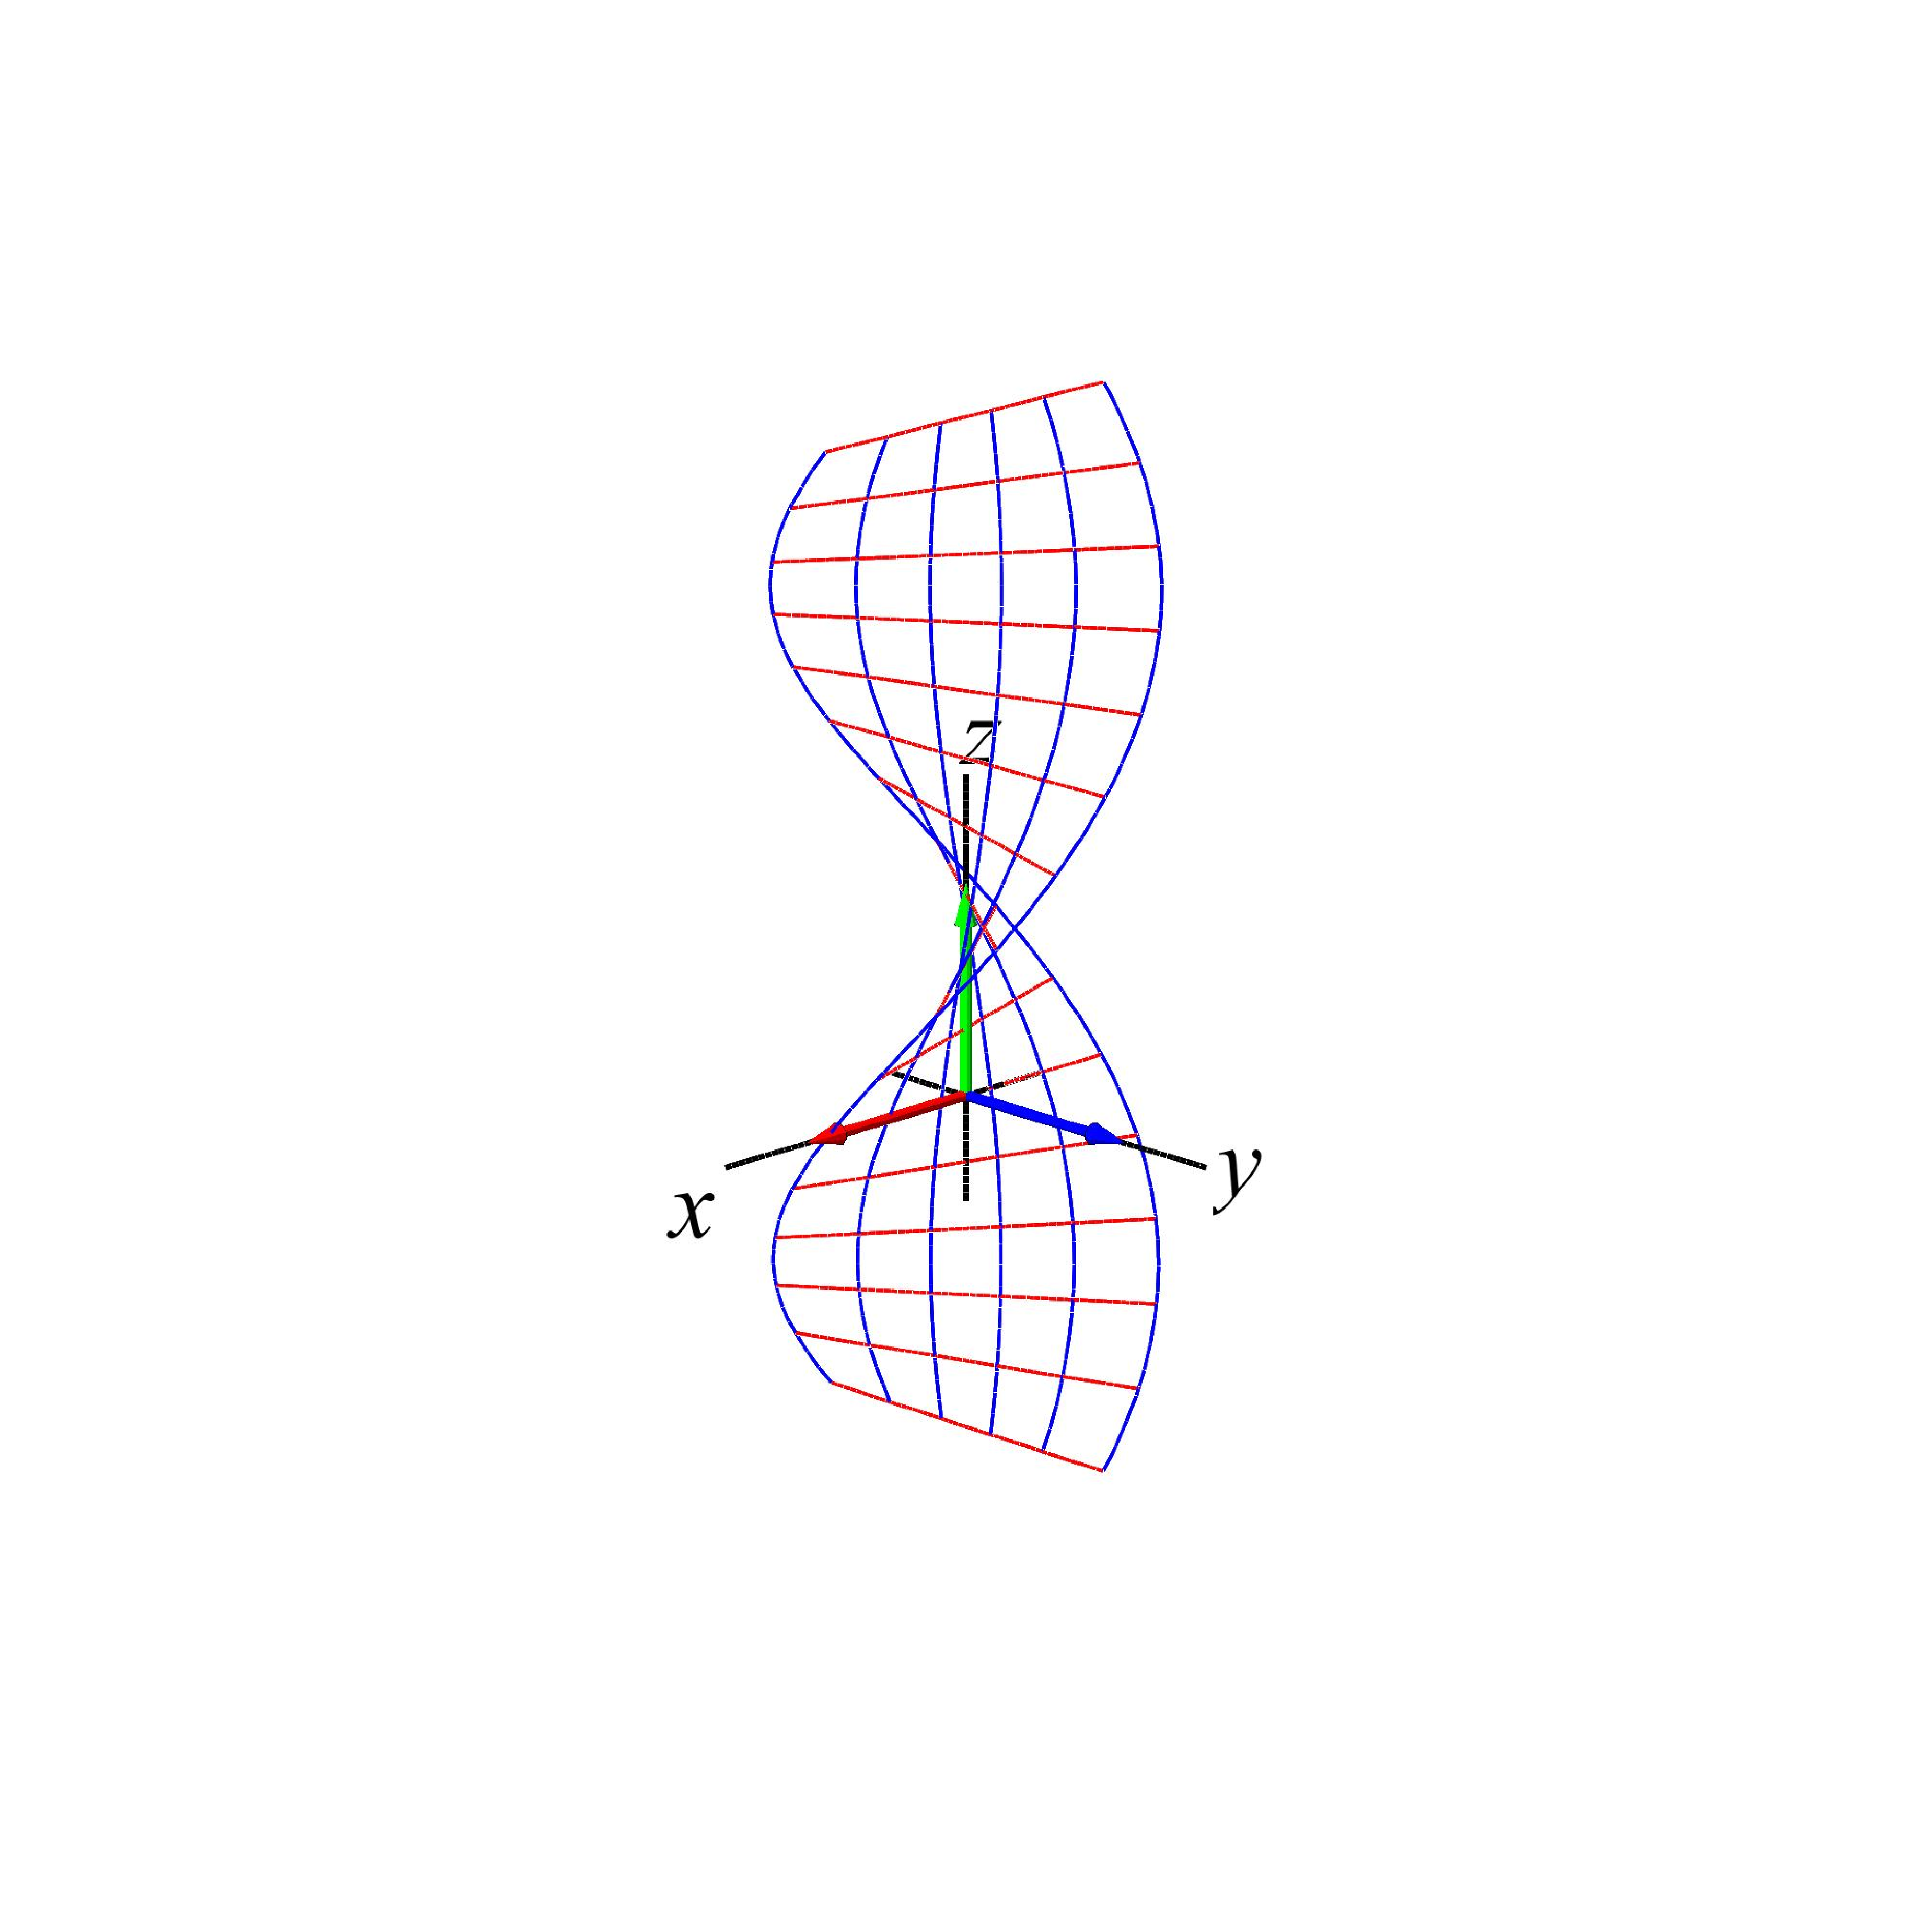
\includegraphics[height=70mm]{FIGS/plotVindel1} 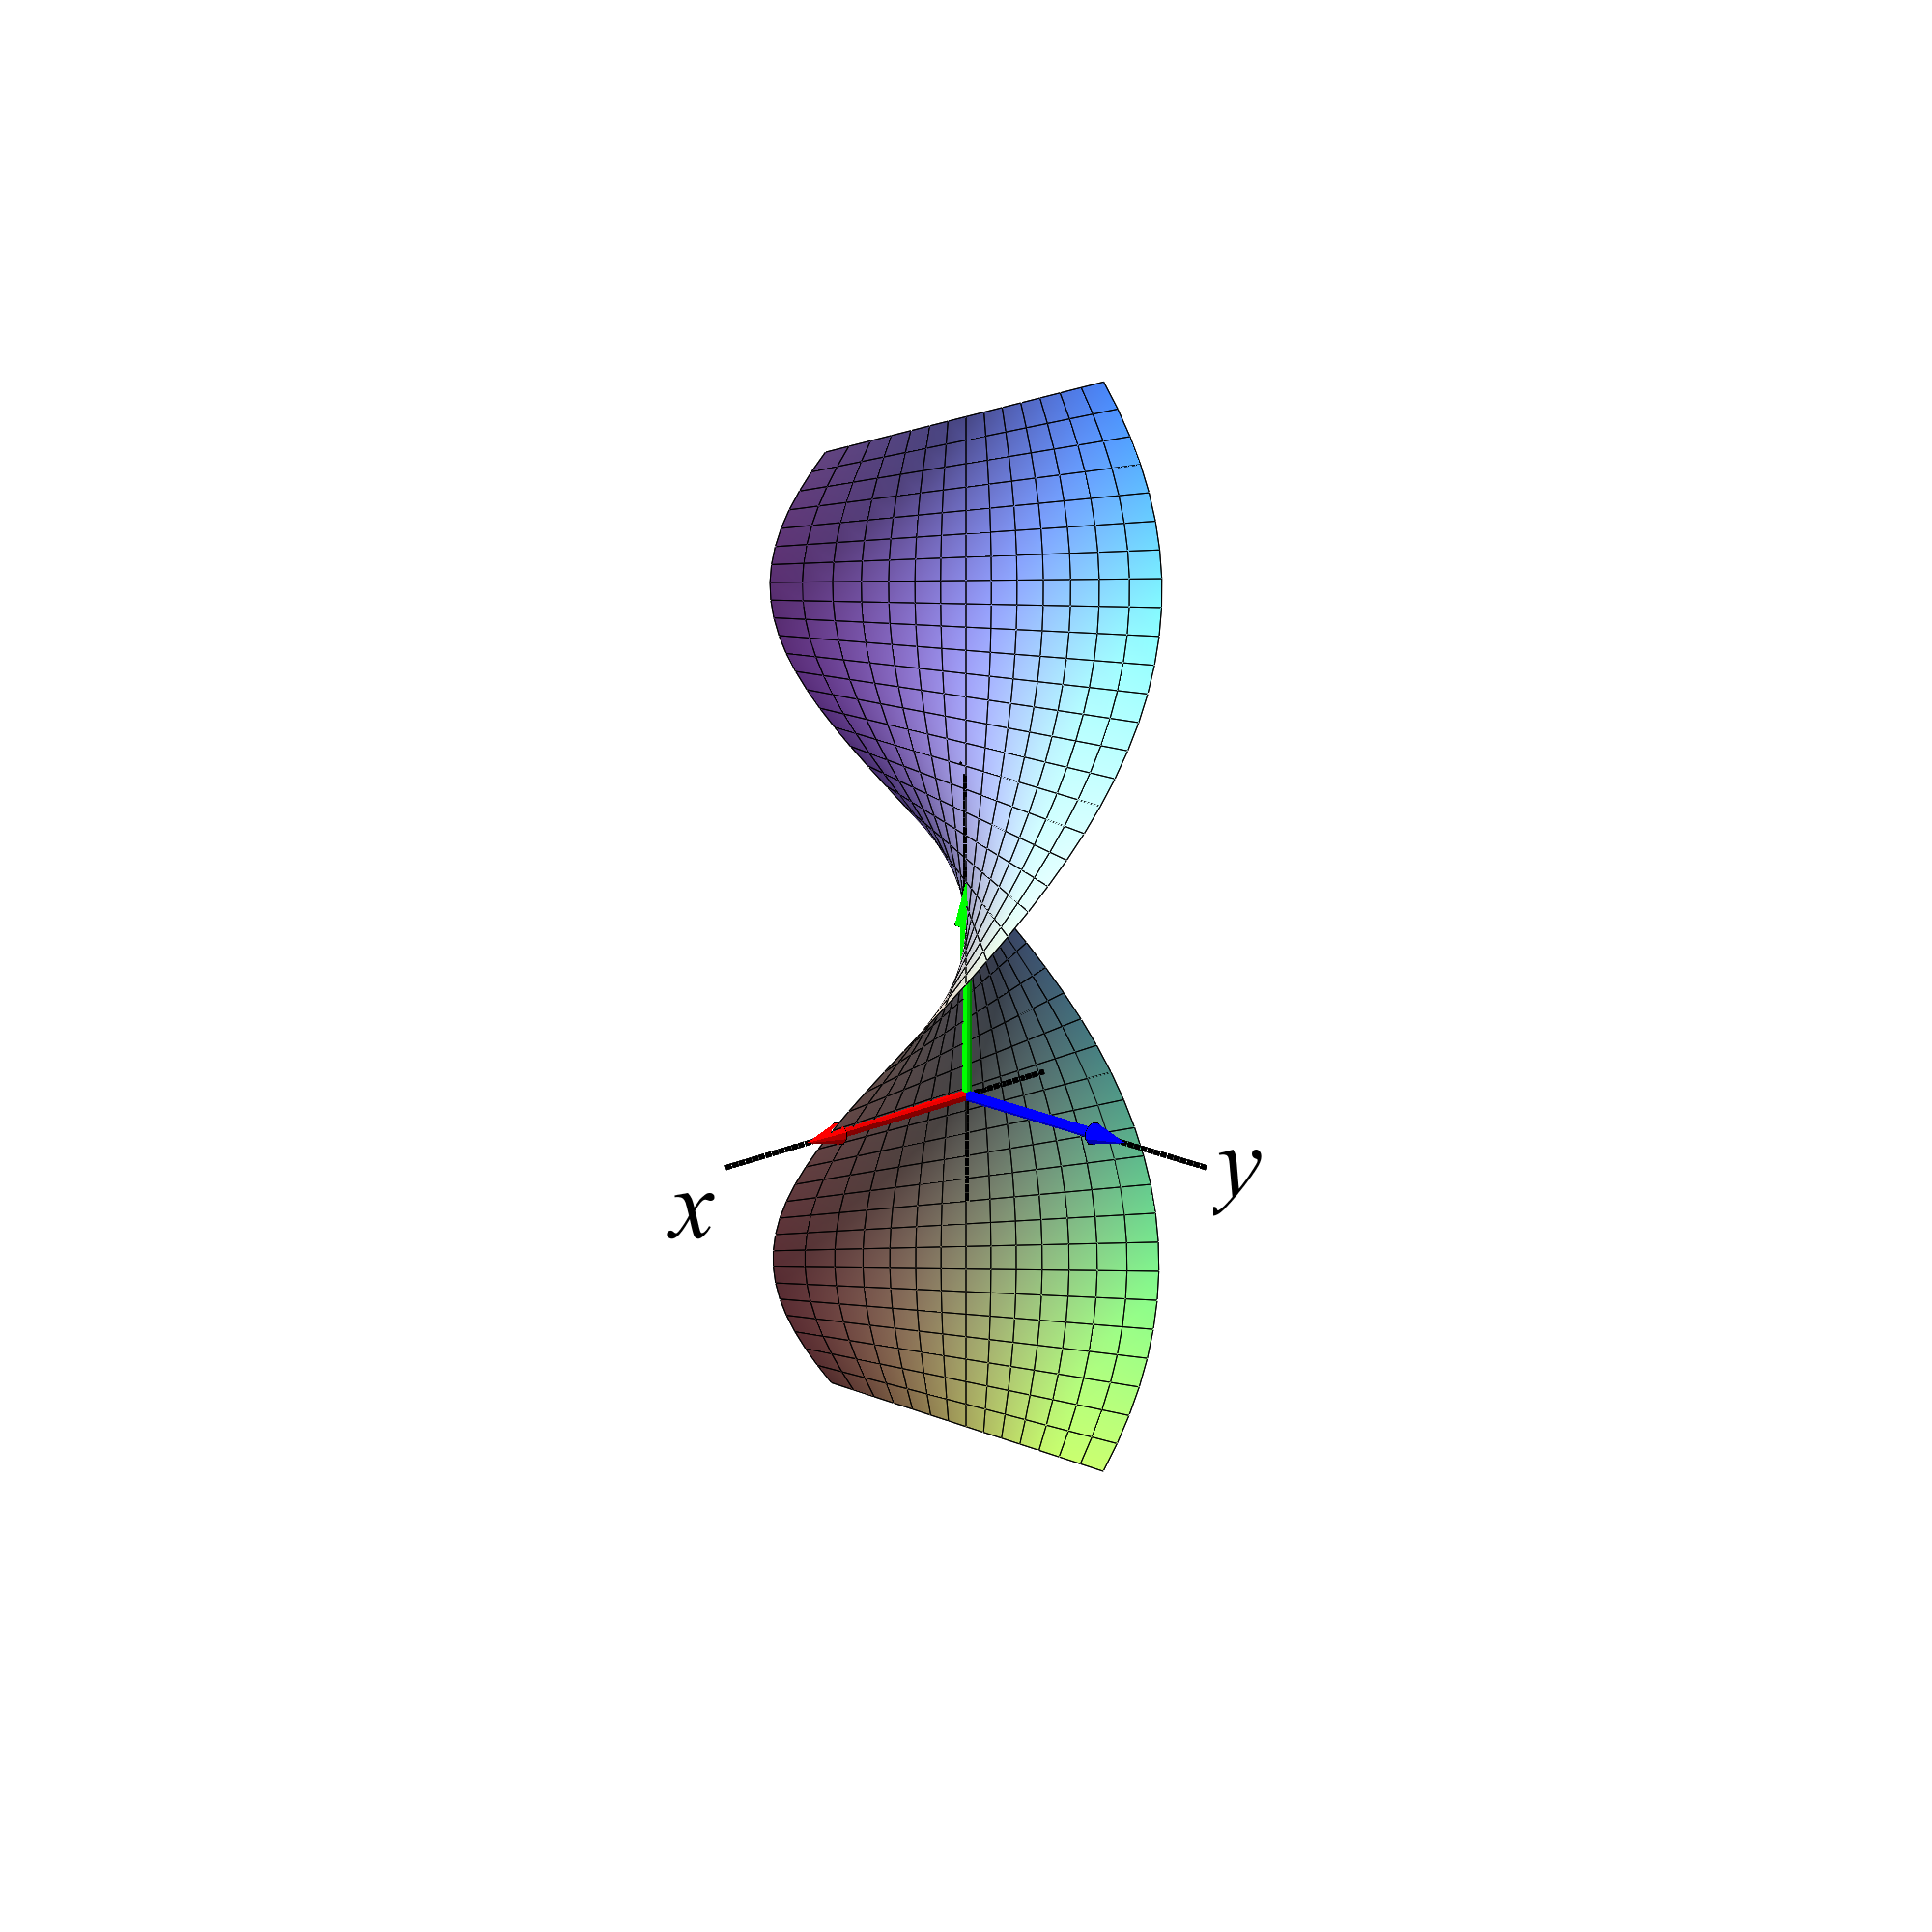
\includegraphics[height=70mm]{FIGS/plotVindel2} 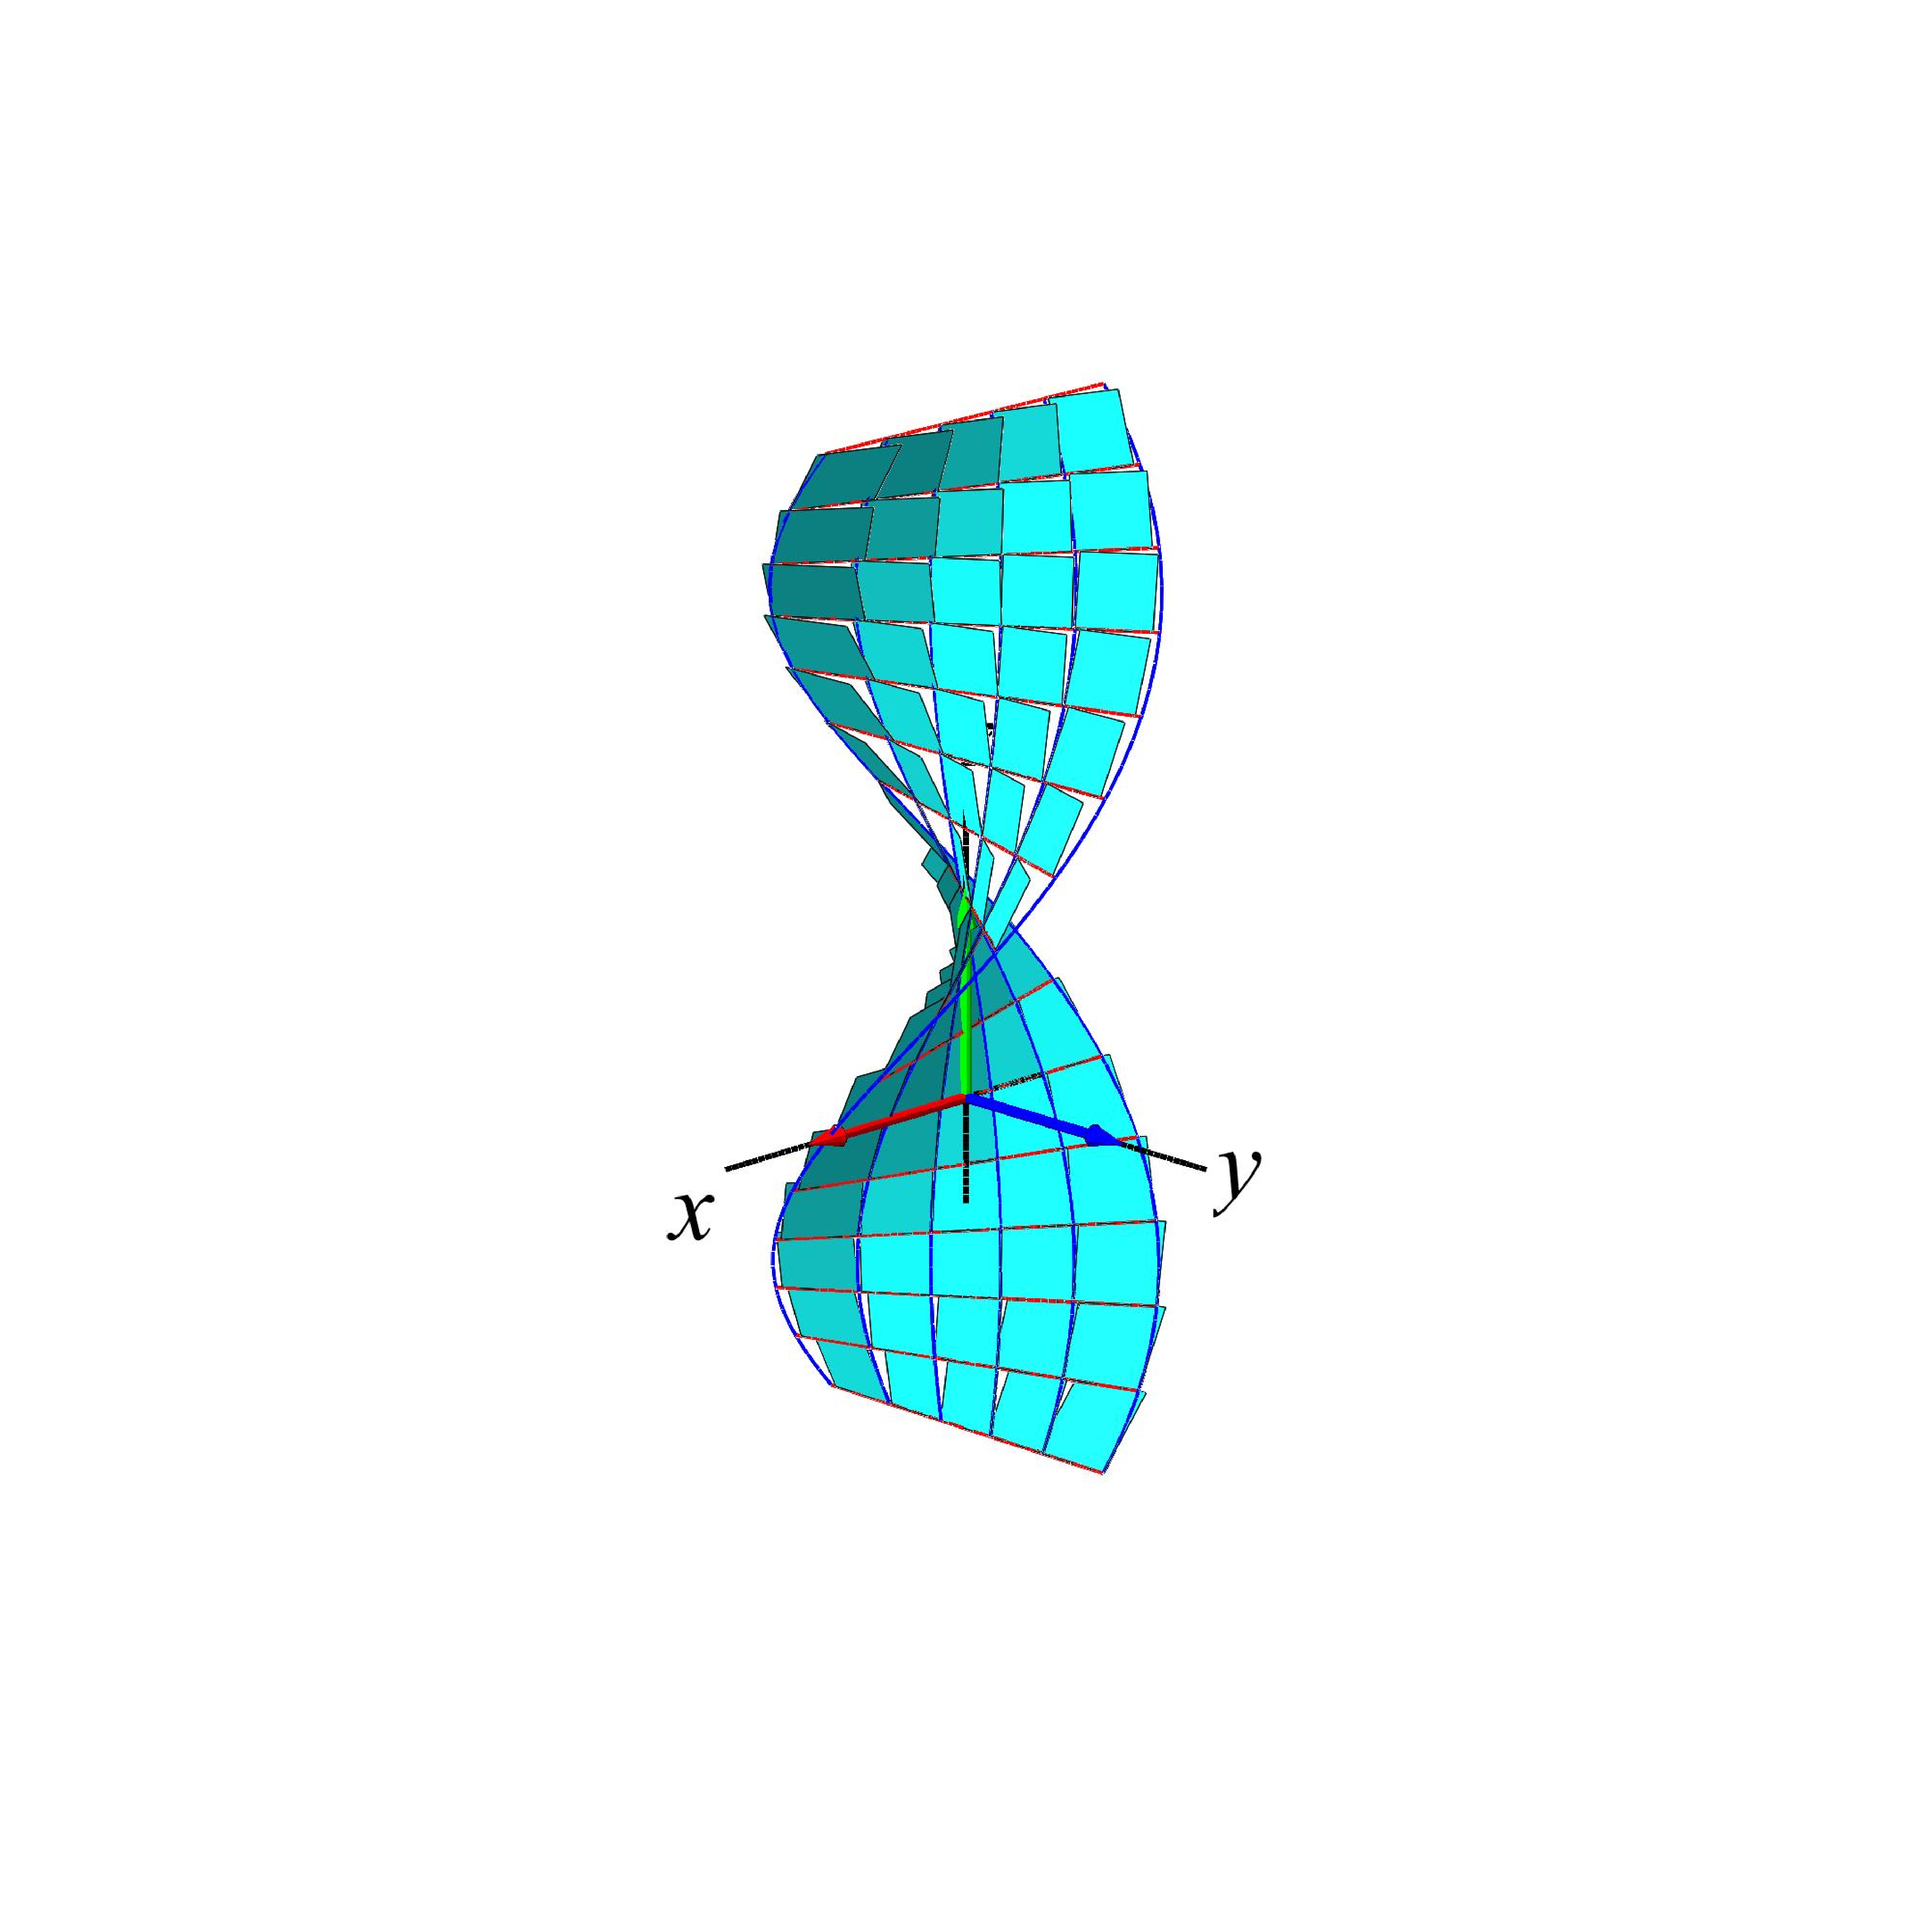
\includegraphics[height=70mm]{FIGS/plotVindel3}   }
\begin{center}
\caption{\small{Denne vindelflade er givet ved
parameterfremstillingen ${\bf r}(u, v) \, = \,
(\sinh(u)\cos(v), \sinh(u)\sin(v), v) \,$.
Figuren viser også en approksimation af fladen med
parallelogrammer, som faktisk alle er \emph{kvadrater}
af forskellig størrelse. Se opgave
\ref{exerVindelApp}.}} \label{figVindel12}
\end{center}
\end{figure}

\begin{exercise}\label{exerVindelApp}
Vis, at de approksimerende parallelogrammer i
figur \ref{figVindel12} alle er kvadrater.
\end{exercise}





\subsubsection{Massen af en flade}\label{subsubsecMasseFlade}
Hvis vi nu antager, at
hvert enkelt parallelogram i (\ref{eqApp2})
tildeles en konstant massetæthed givet ved
værdien af funktionen $f(x,y,z)$ i
parallelogrammets kontaktpunkt med fladen, så får
vi massen af det $(i, j)$'te parallelogram :
\begin{equation}
\begin{aligned}
\Delta \M_{ij} \, &= \, f(x(u_{i}, v_{j}), y(u_{i}, v_{j}), z(u_{i},
v_{j})) \, \Jac_{\bf r}(u_{i}, v_{j}) \cdot\delta_{u} \delta_{v} \, \\
&= \, f( {\bf r}(u_{i}, v_{j})) \, \Jac_{\bf r}(u_{i}, v_{j})
\cdot\delta_{u} \delta_{v}\quad .
\end{aligned}
\end{equation}
Den totale masse af hele systemet af
parallelogrammer er derfor følgende, som er en
god ap\-proksimation til massen af hele fladen
når denne gives massetætheden $f({\bf r}(u,v))$ i
punktet ${\bf r}(u,v)$.
\begin{equation}
\M_{\app}(n,m) \, = \,  \sum_{j=1}^{m} \sum_{i=1}^{n} \Delta \M_{ij} \,
= \, \sum_{j=1}^{m}\sum_{i=1}^{n}f({\bf r}(u_{i},
v_{j}))\,\Jac_{\bf r}(u_{i}, v_{j}) \cdot \delta_{u} \delta_{v}
\quad .
\end{equation}

Dette er en dobbelt integralsum for den kontinuerte funktion $f({\bf
r}(u,v))\,\Jac_{\bf r}(u, v)$ over parameter-rektanglet $\,[a,
b]\times[c, d]\,$. Vi får altså i grænsen, hvor $n$ og $m$ går mod
uendelig:
\begin{equation}
\M_{\app}(n,m)\, \to \, \M \, = \, \int_{c}^{d}\int_{a}^{b}f({\bf r}(u,
v ))\Jac_{\bf r}(u, v)\,du \,dv \quad \text{for} \quad n\, , \, m \to
\infty \quad.
\end{equation}

Dermed har vi motiveret definitionen af massen af en
parametriseret flade med massetætheden $f({\bf r}(u, v))$ og
dermed også den generelle definition af fladeintegralet,
definition \ref{defFladeInt}.

%%%%%%%%%%%%%%%%%%%%%%%%%%%%%%%%%%%%%%%%

\subsection{Omdrejningsflader} \label{subsecOmdrejningsflader}
Omdrejningsflader er de specielle flader, der
fremkommer ved at dreje en plan kurve omkring en
ret linje (omdrejningsaksen) som også ligger i
samme plan. Kurven kaldes en {\em{{profil-kurve}}}
eller en {\em{{frembringer-kurve}}}. Det antages,
at profilkurven ikke skærer omdrejningsaksen.
Profilkurven vælges typisk i $(x, z)$-planen og
drejes om $z$-aksen i et
$\,(x,y,z)$-koordinatsystem. Profil-kurven kan så
repræsenteres ved en parameterfremstilling
således:
\begin{equation}
G_{\bf p} : \quad {\bf p}(u) \, = \, \left(g(u), 0, h(u)\right)
\in \mathbb{R}^3 \quad , \, \, \,  u \in [a,b] \quad,
\end{equation}
hvor $g(u)\, > \, 0$  og $h(u)$ er givne
funktioner af parameteren $u$. Den
omdrejningsflade, der fremkommer ved at dreje
$G_{\bf p}$ en hel gang omkring $z$-aksen har
derfor parameterfremstillingen:
\begin{equation} \label{eqFG}
FG_{\bf r} : \quad {\bf r}(u,v) \, = \, \left(g(u)\cos(v), g(u)\sin(v),
h(u)\right) \, \, , \, \, \,  u \in [a,b] \, \,
, \, \,  v \in [-\pi, \pi] \quad.
\end{equation}


\begin{figure}[h]
\centerline{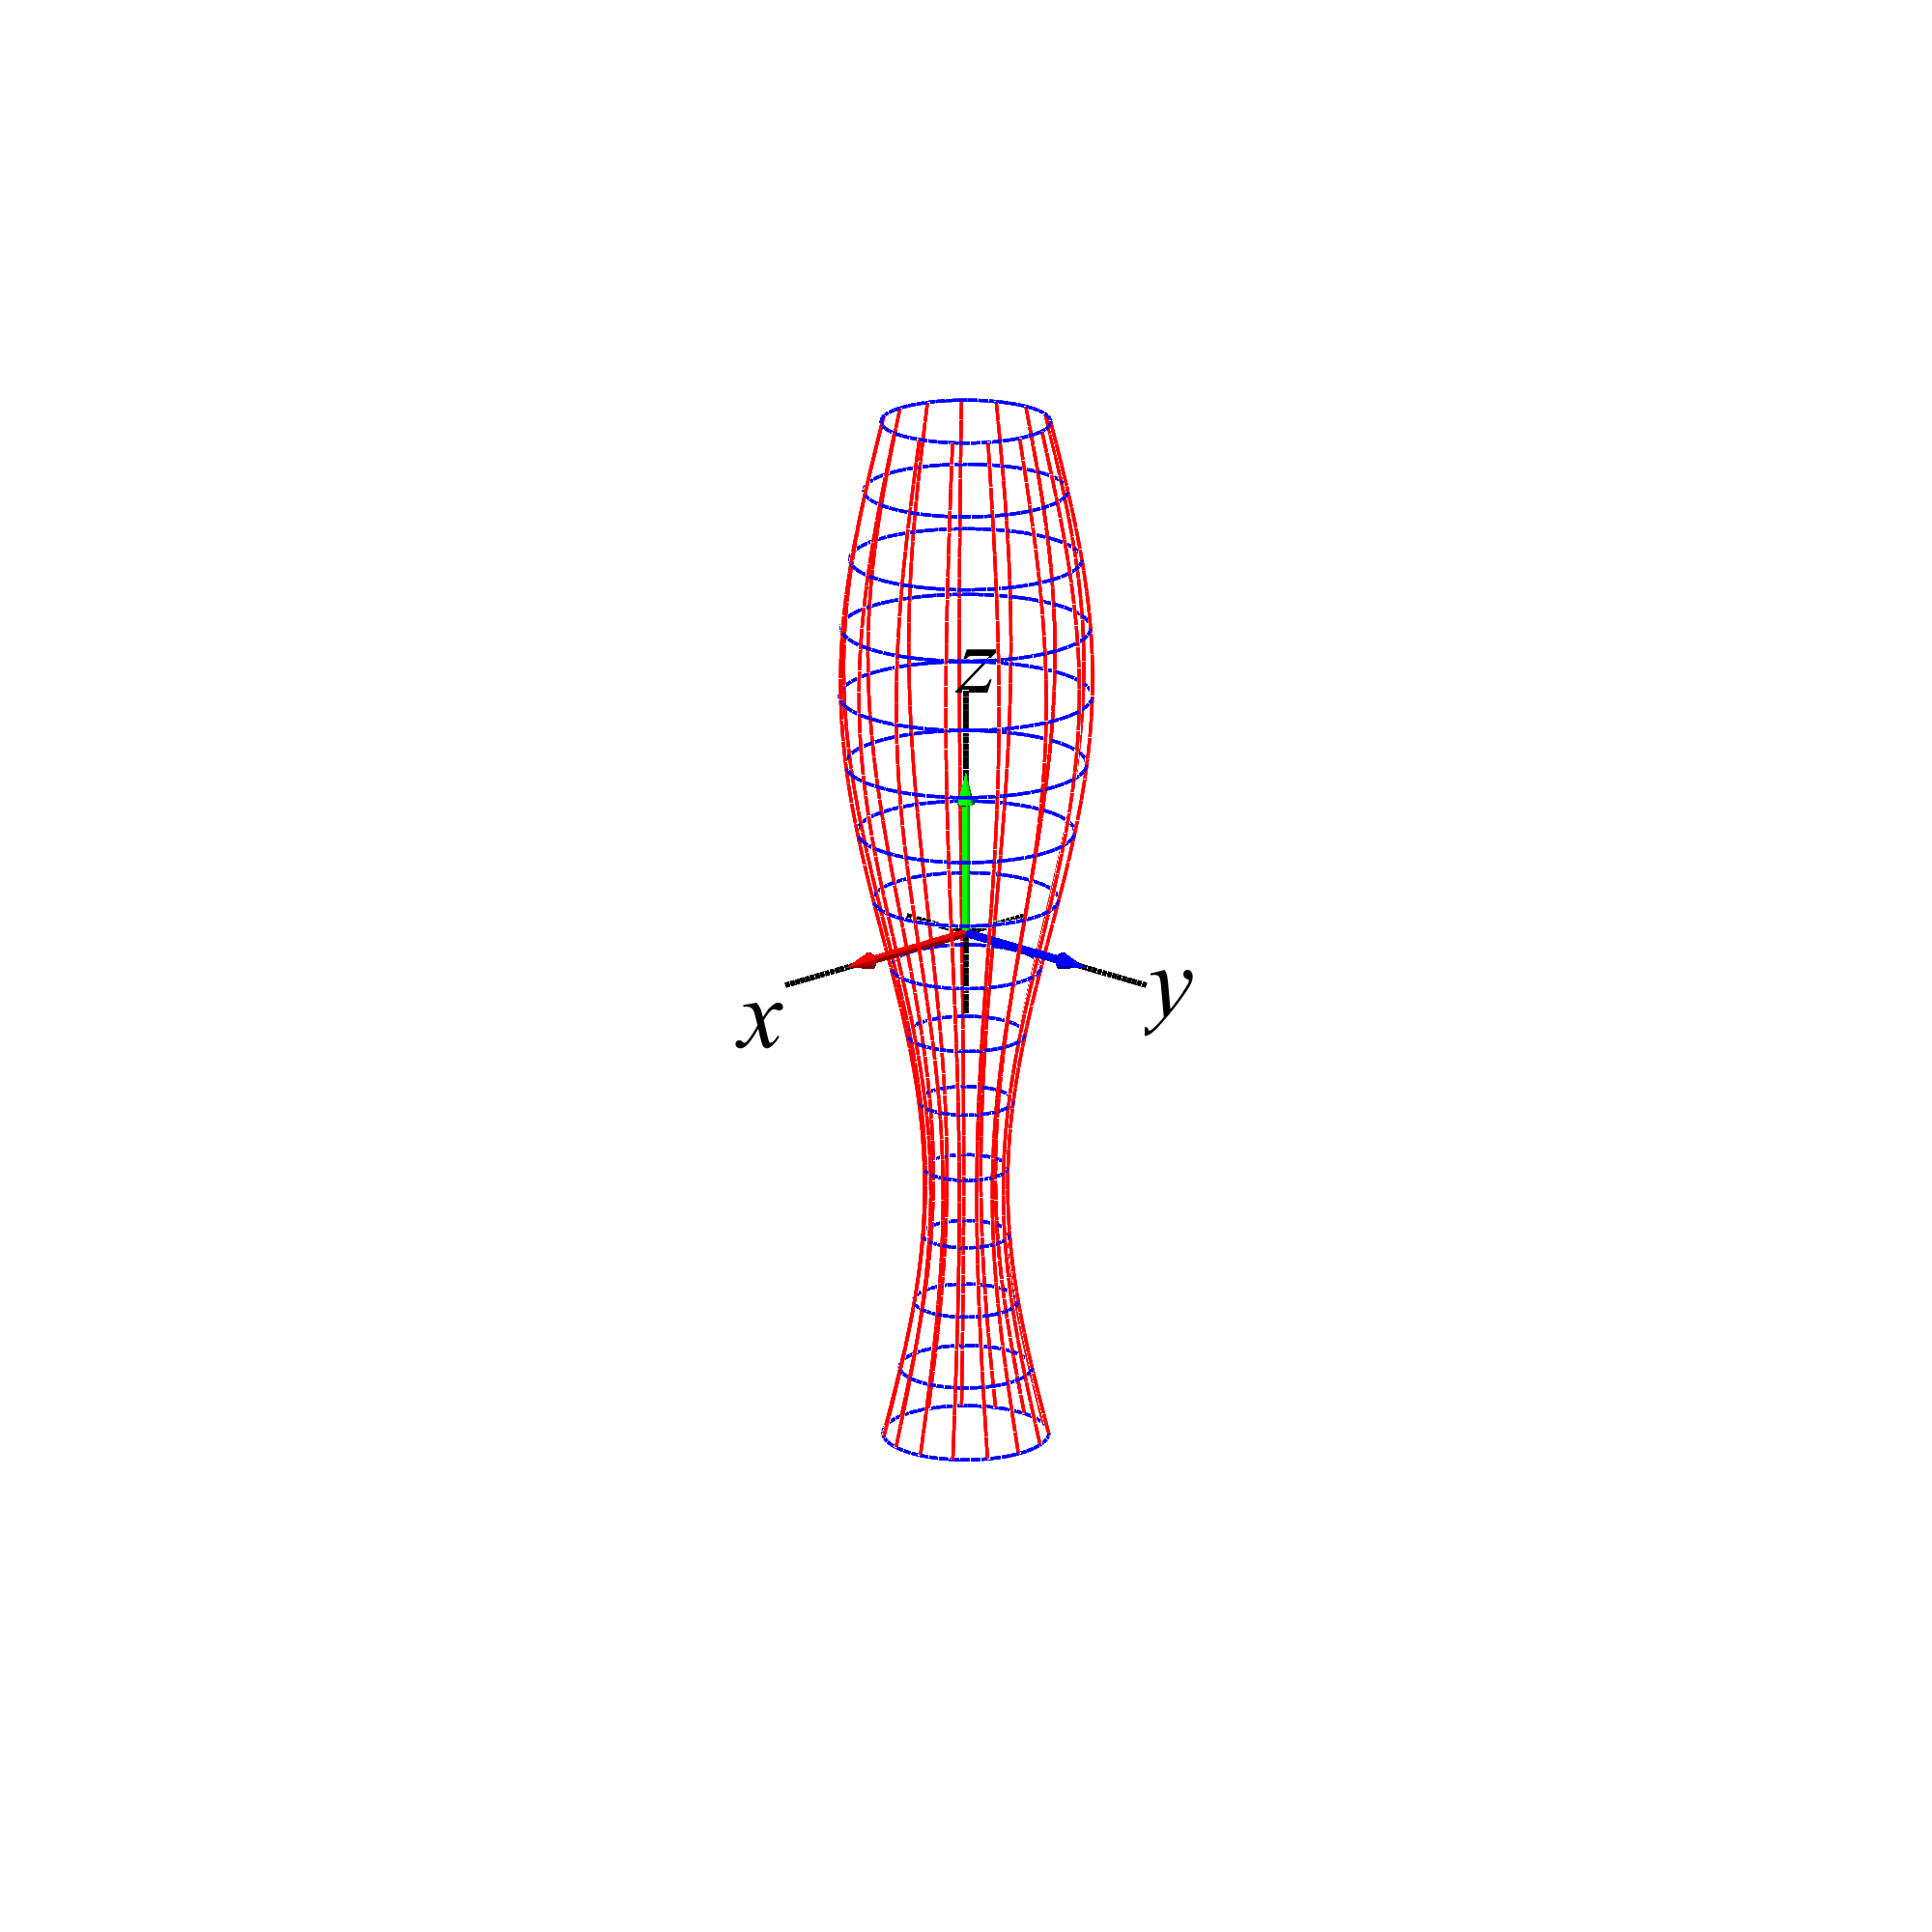
\includegraphics[height=60mm]{FIGS/plotRevo1} 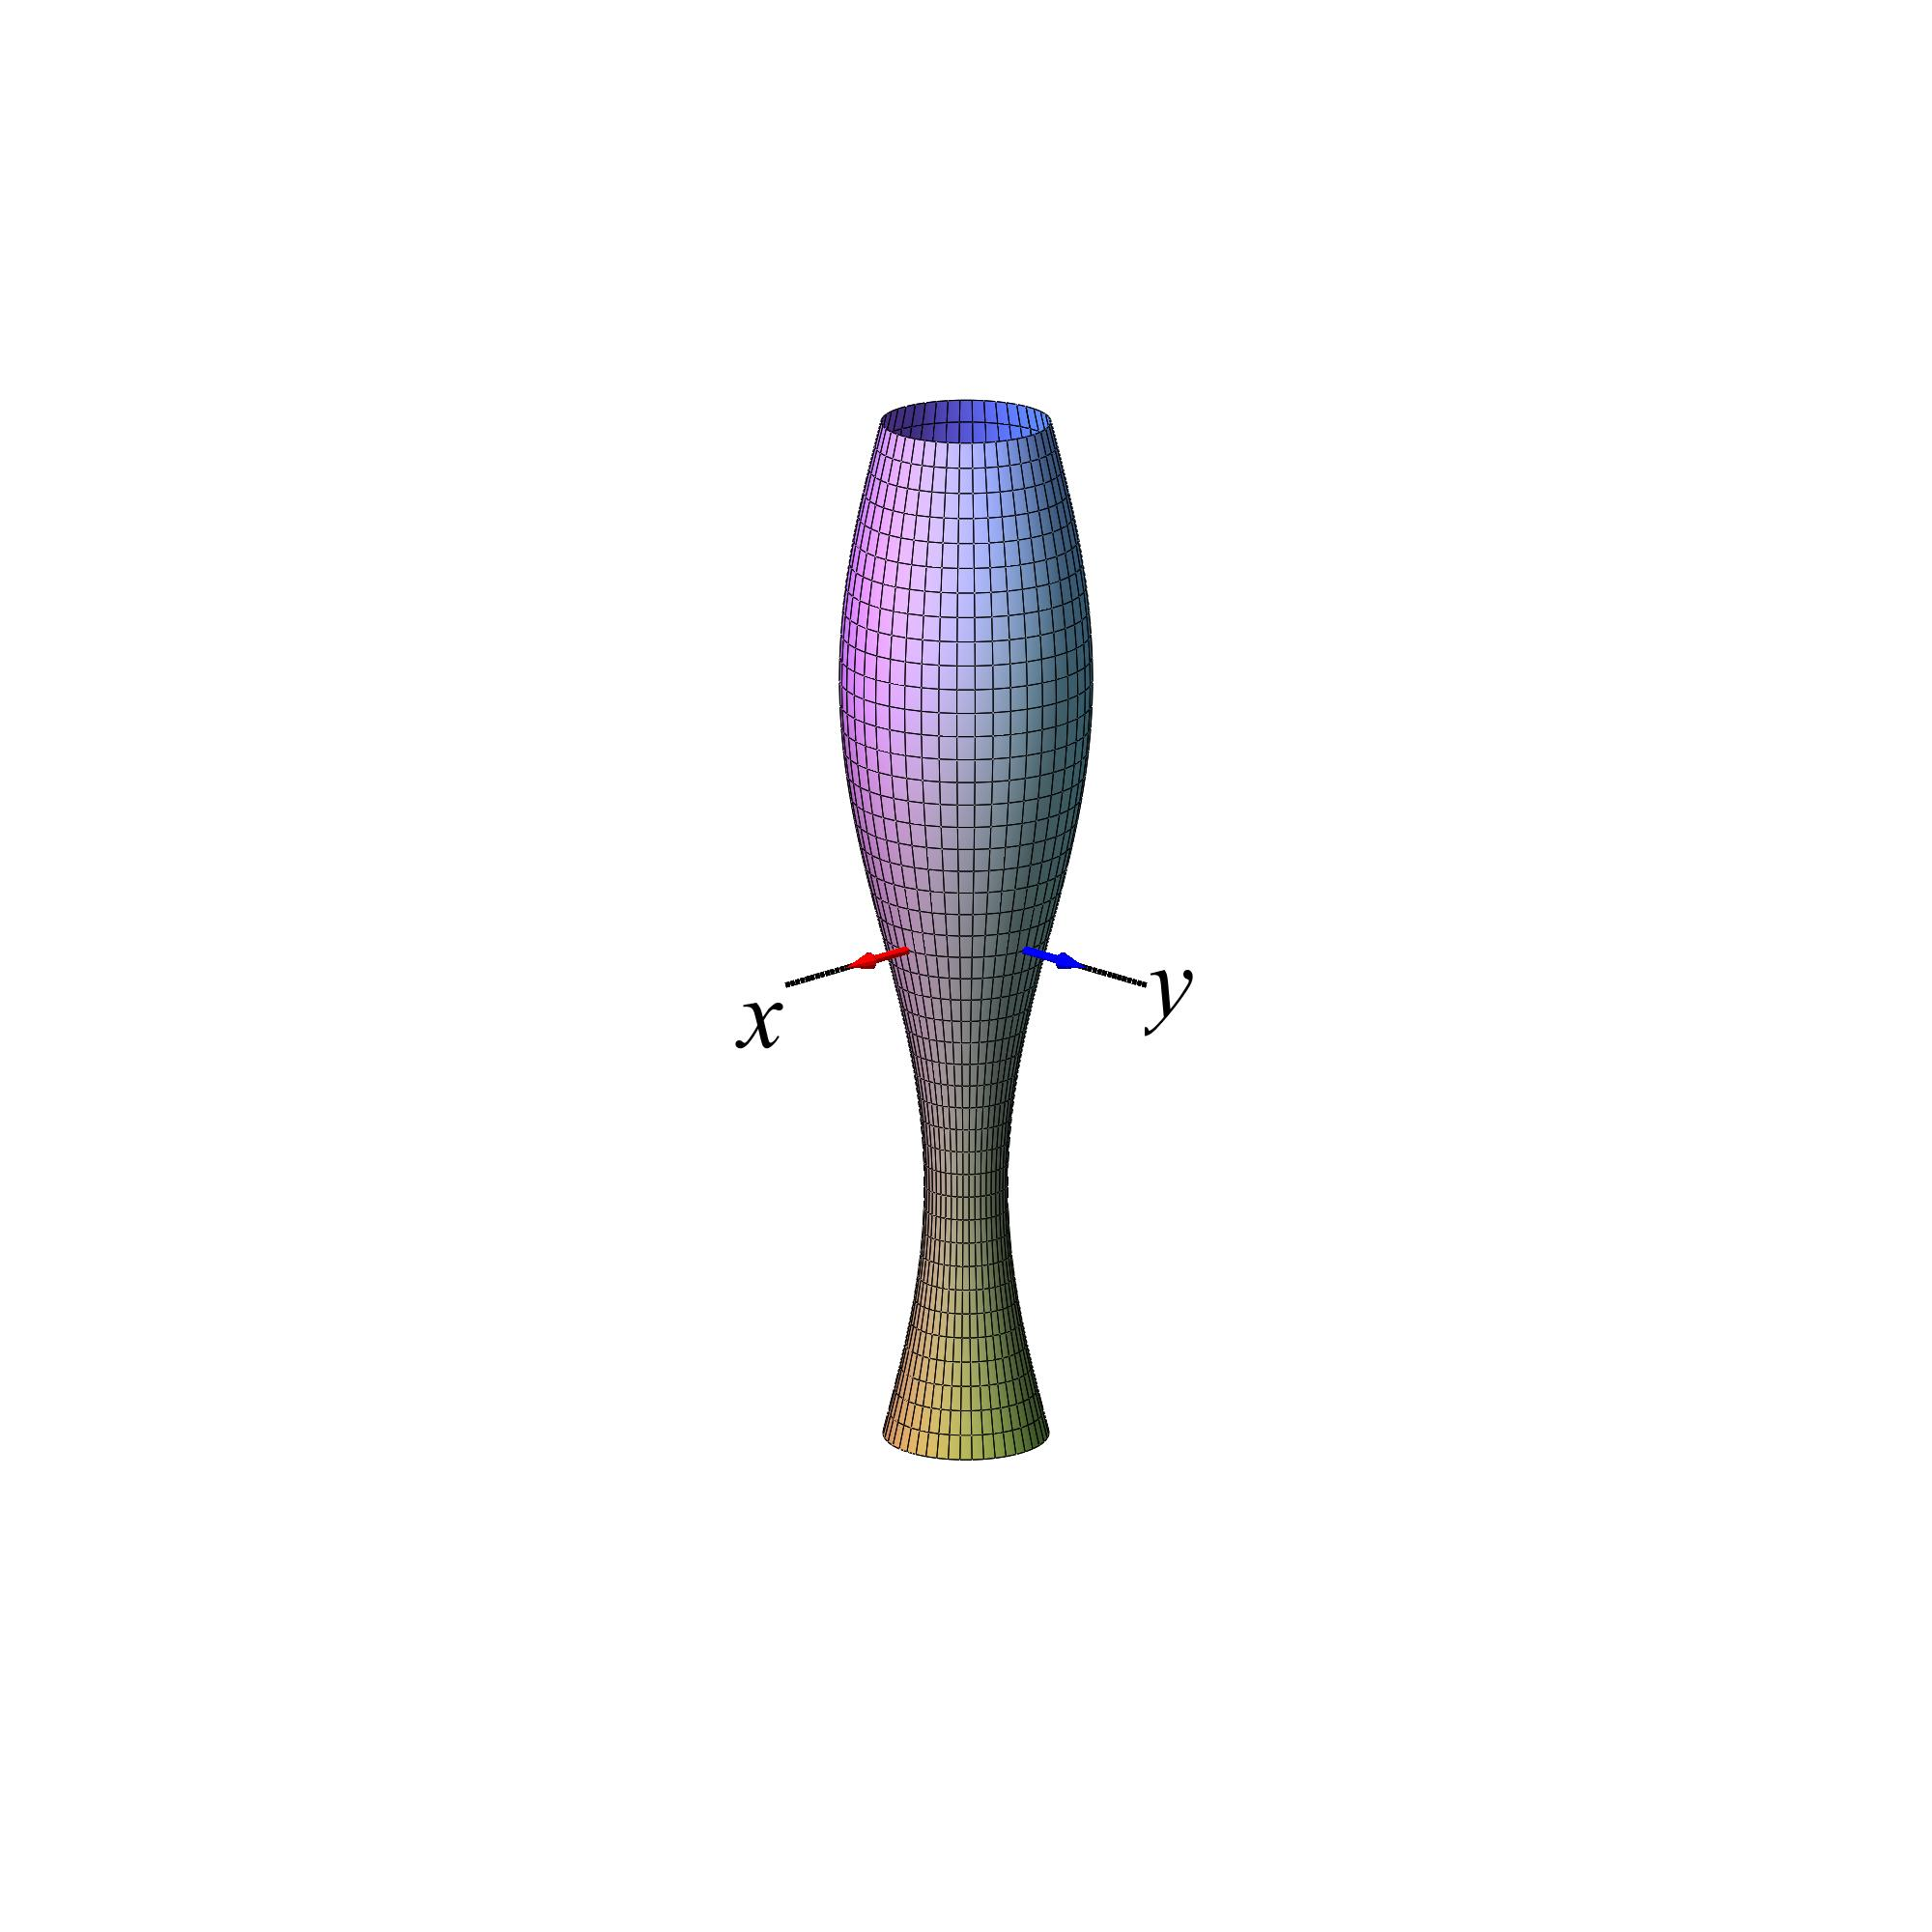
\includegraphics[height=60mm]{FIGS/plotRevo2} 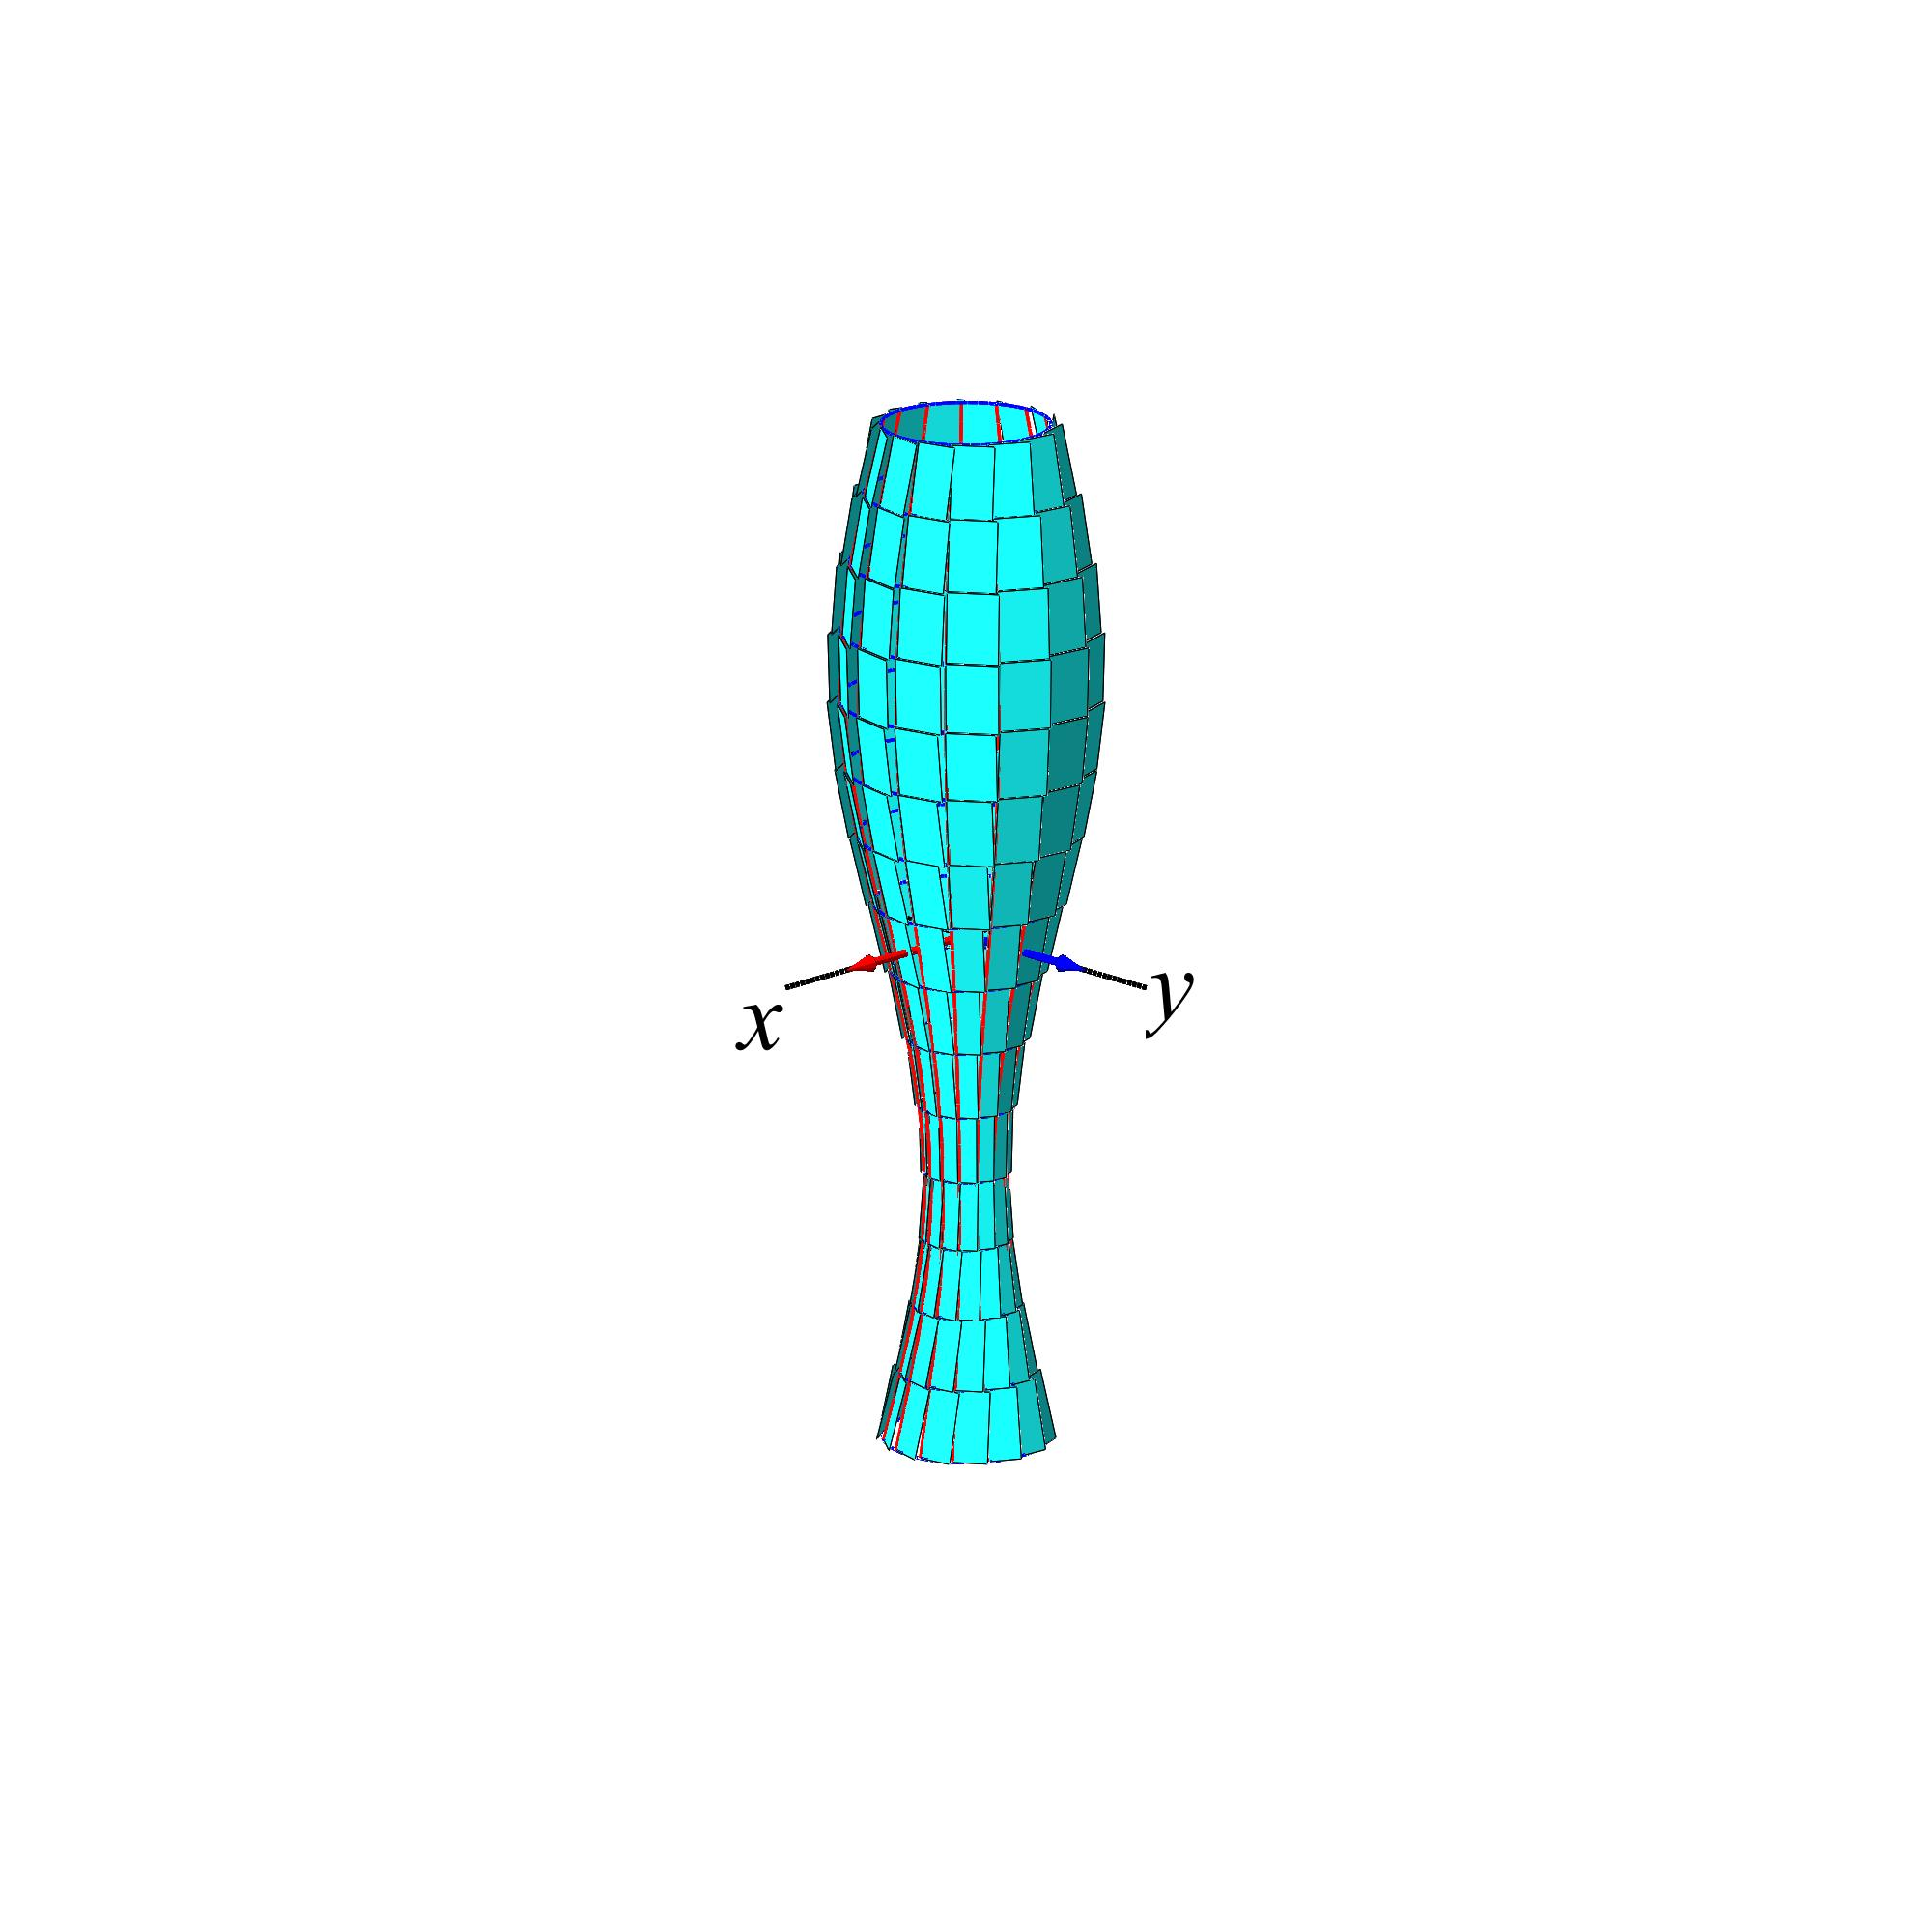
\includegraphics[height=60mm]{FIGS/plotRevo3} }
\begin{center}
\caption{\small{Omdrejnings-fladen her er givet
ved parameterfremstillingen ${\bf r}(u, v) \, =
\, (g(u)\cos(v), g(u)\sin(v), h(u)) \,\,, \,\, u
\in [-\pi, \pi ]\,\, , \, \, v \in [-\pi, \pi]$,
hvor $g(u) = \frac{1}{2} + \frac{1}{4}\sin(u)$ og
$h(u) = u$.}} \label{figOmdrej12}
\end{center}
\end{figure}



\begin{figure}[h]
\centerline{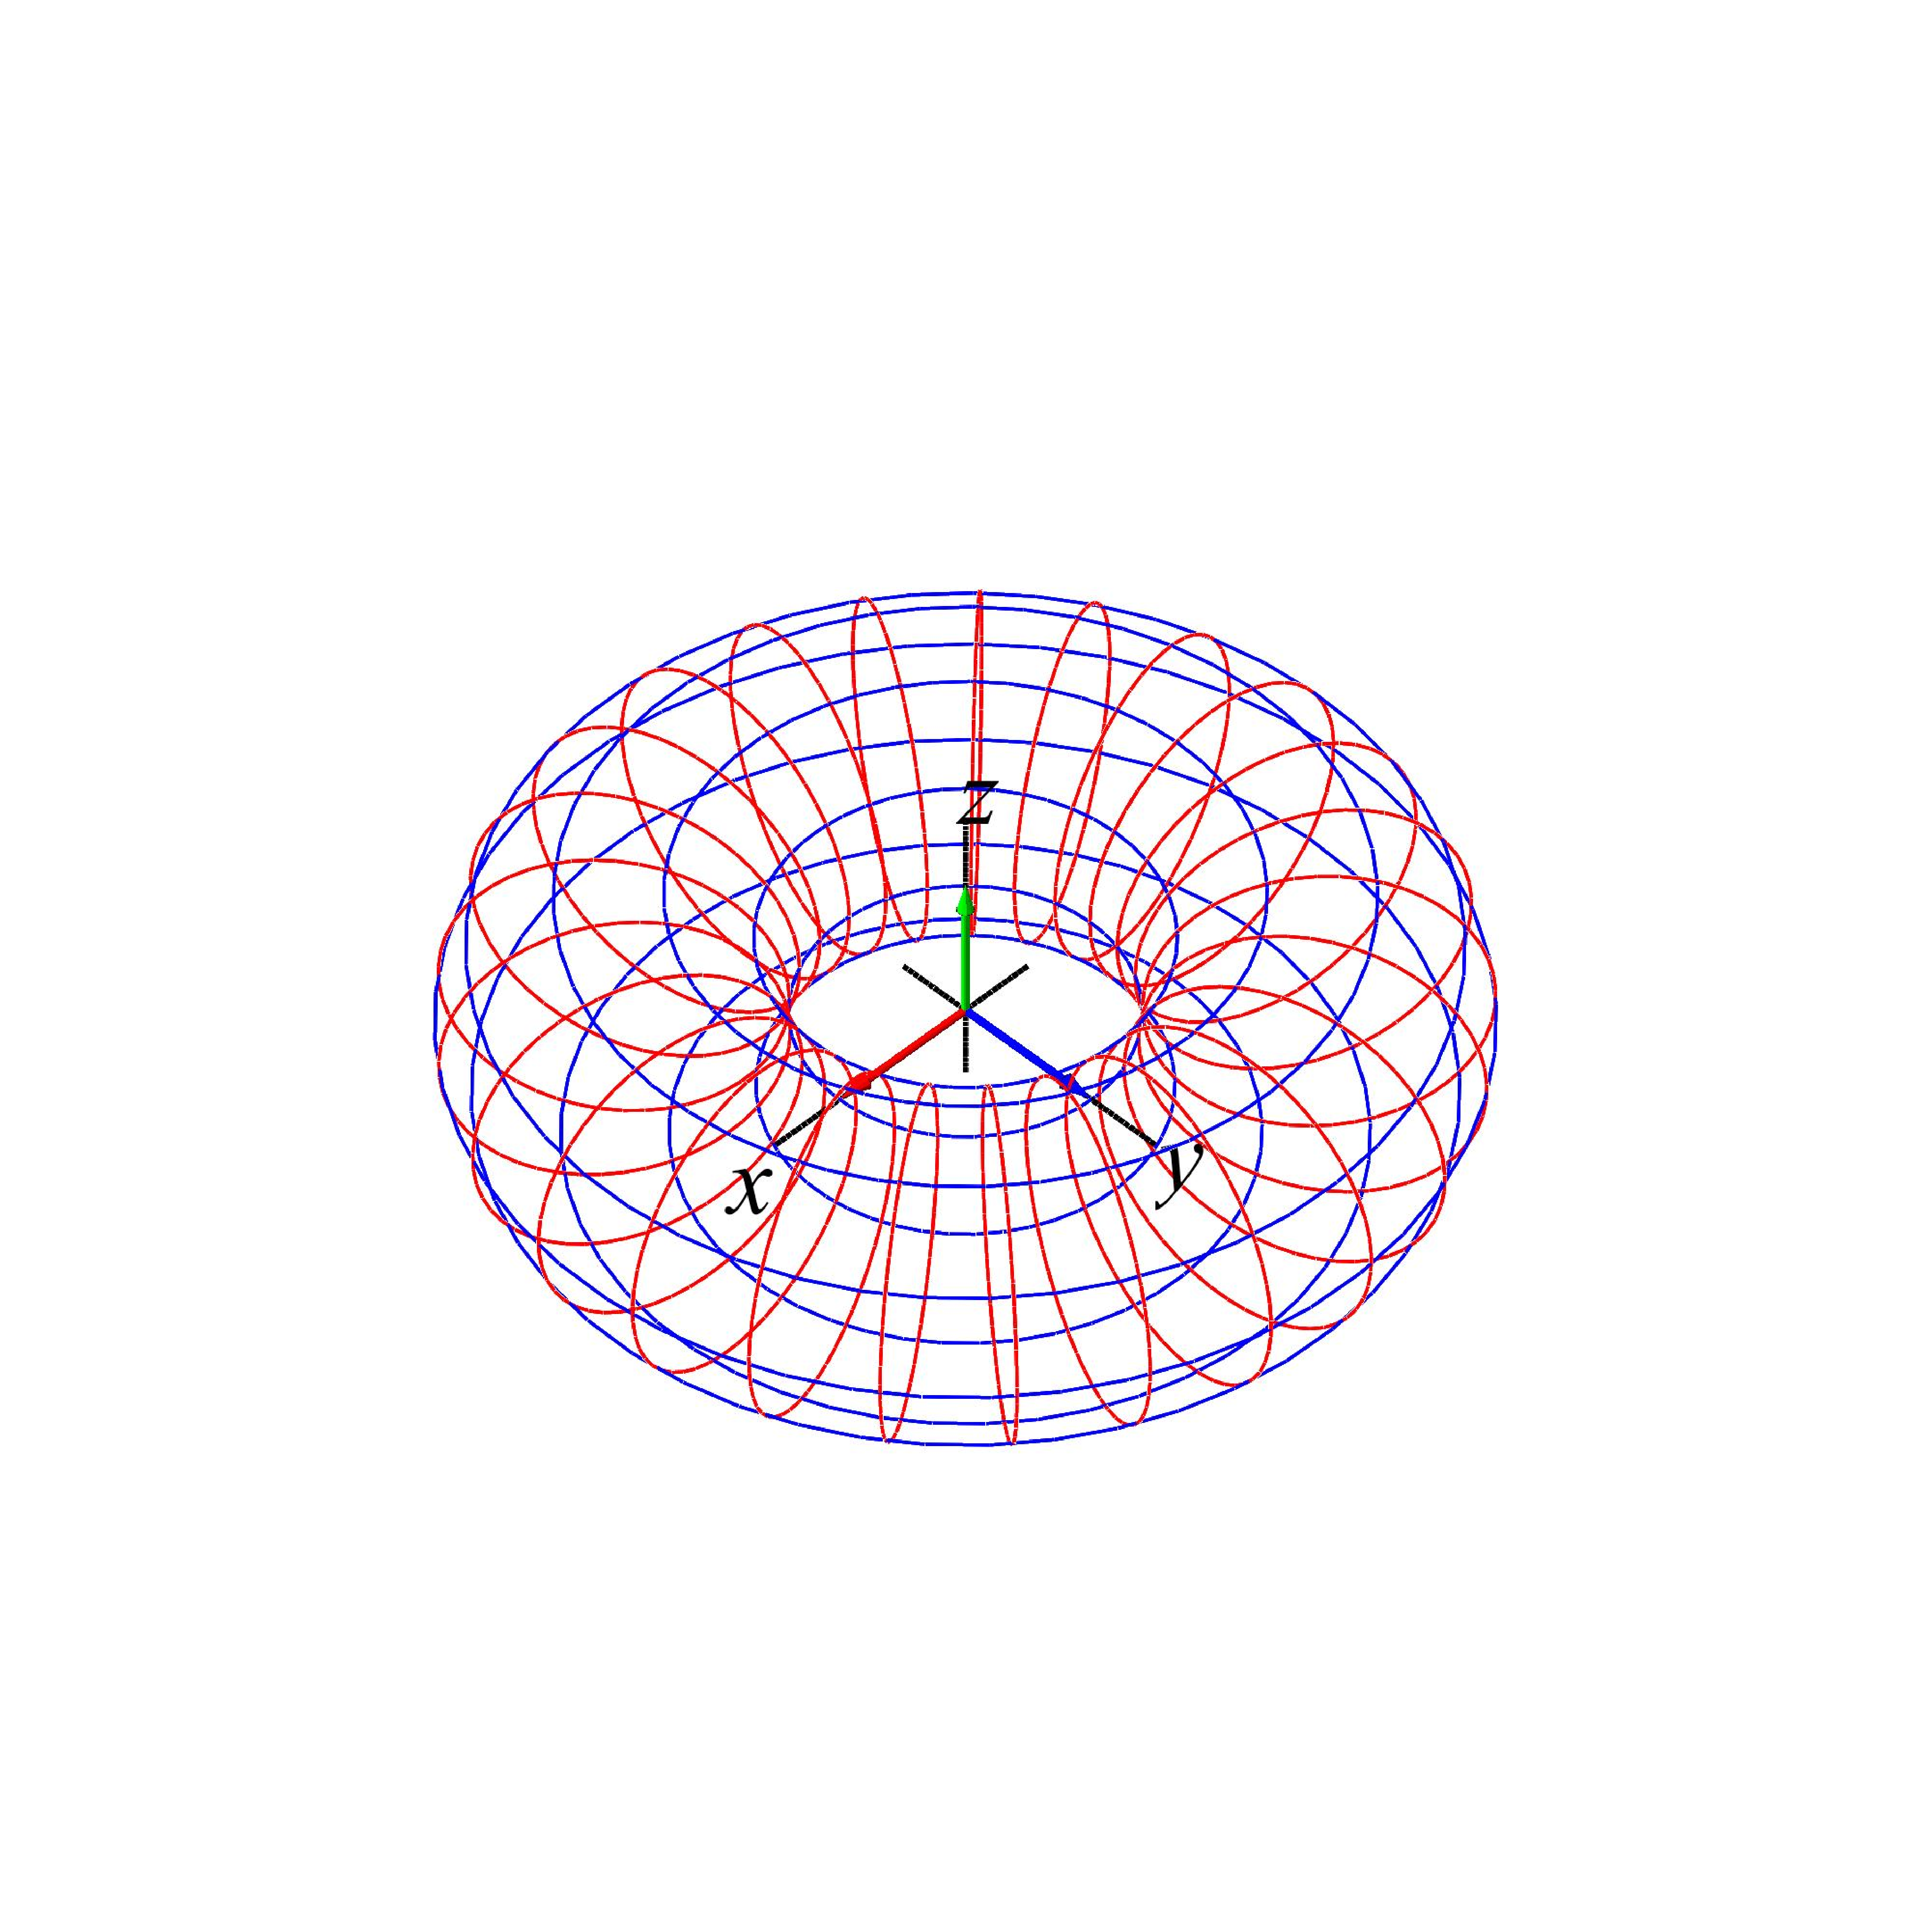
\includegraphics[height=60mm]{FIGS/plotTorus1} 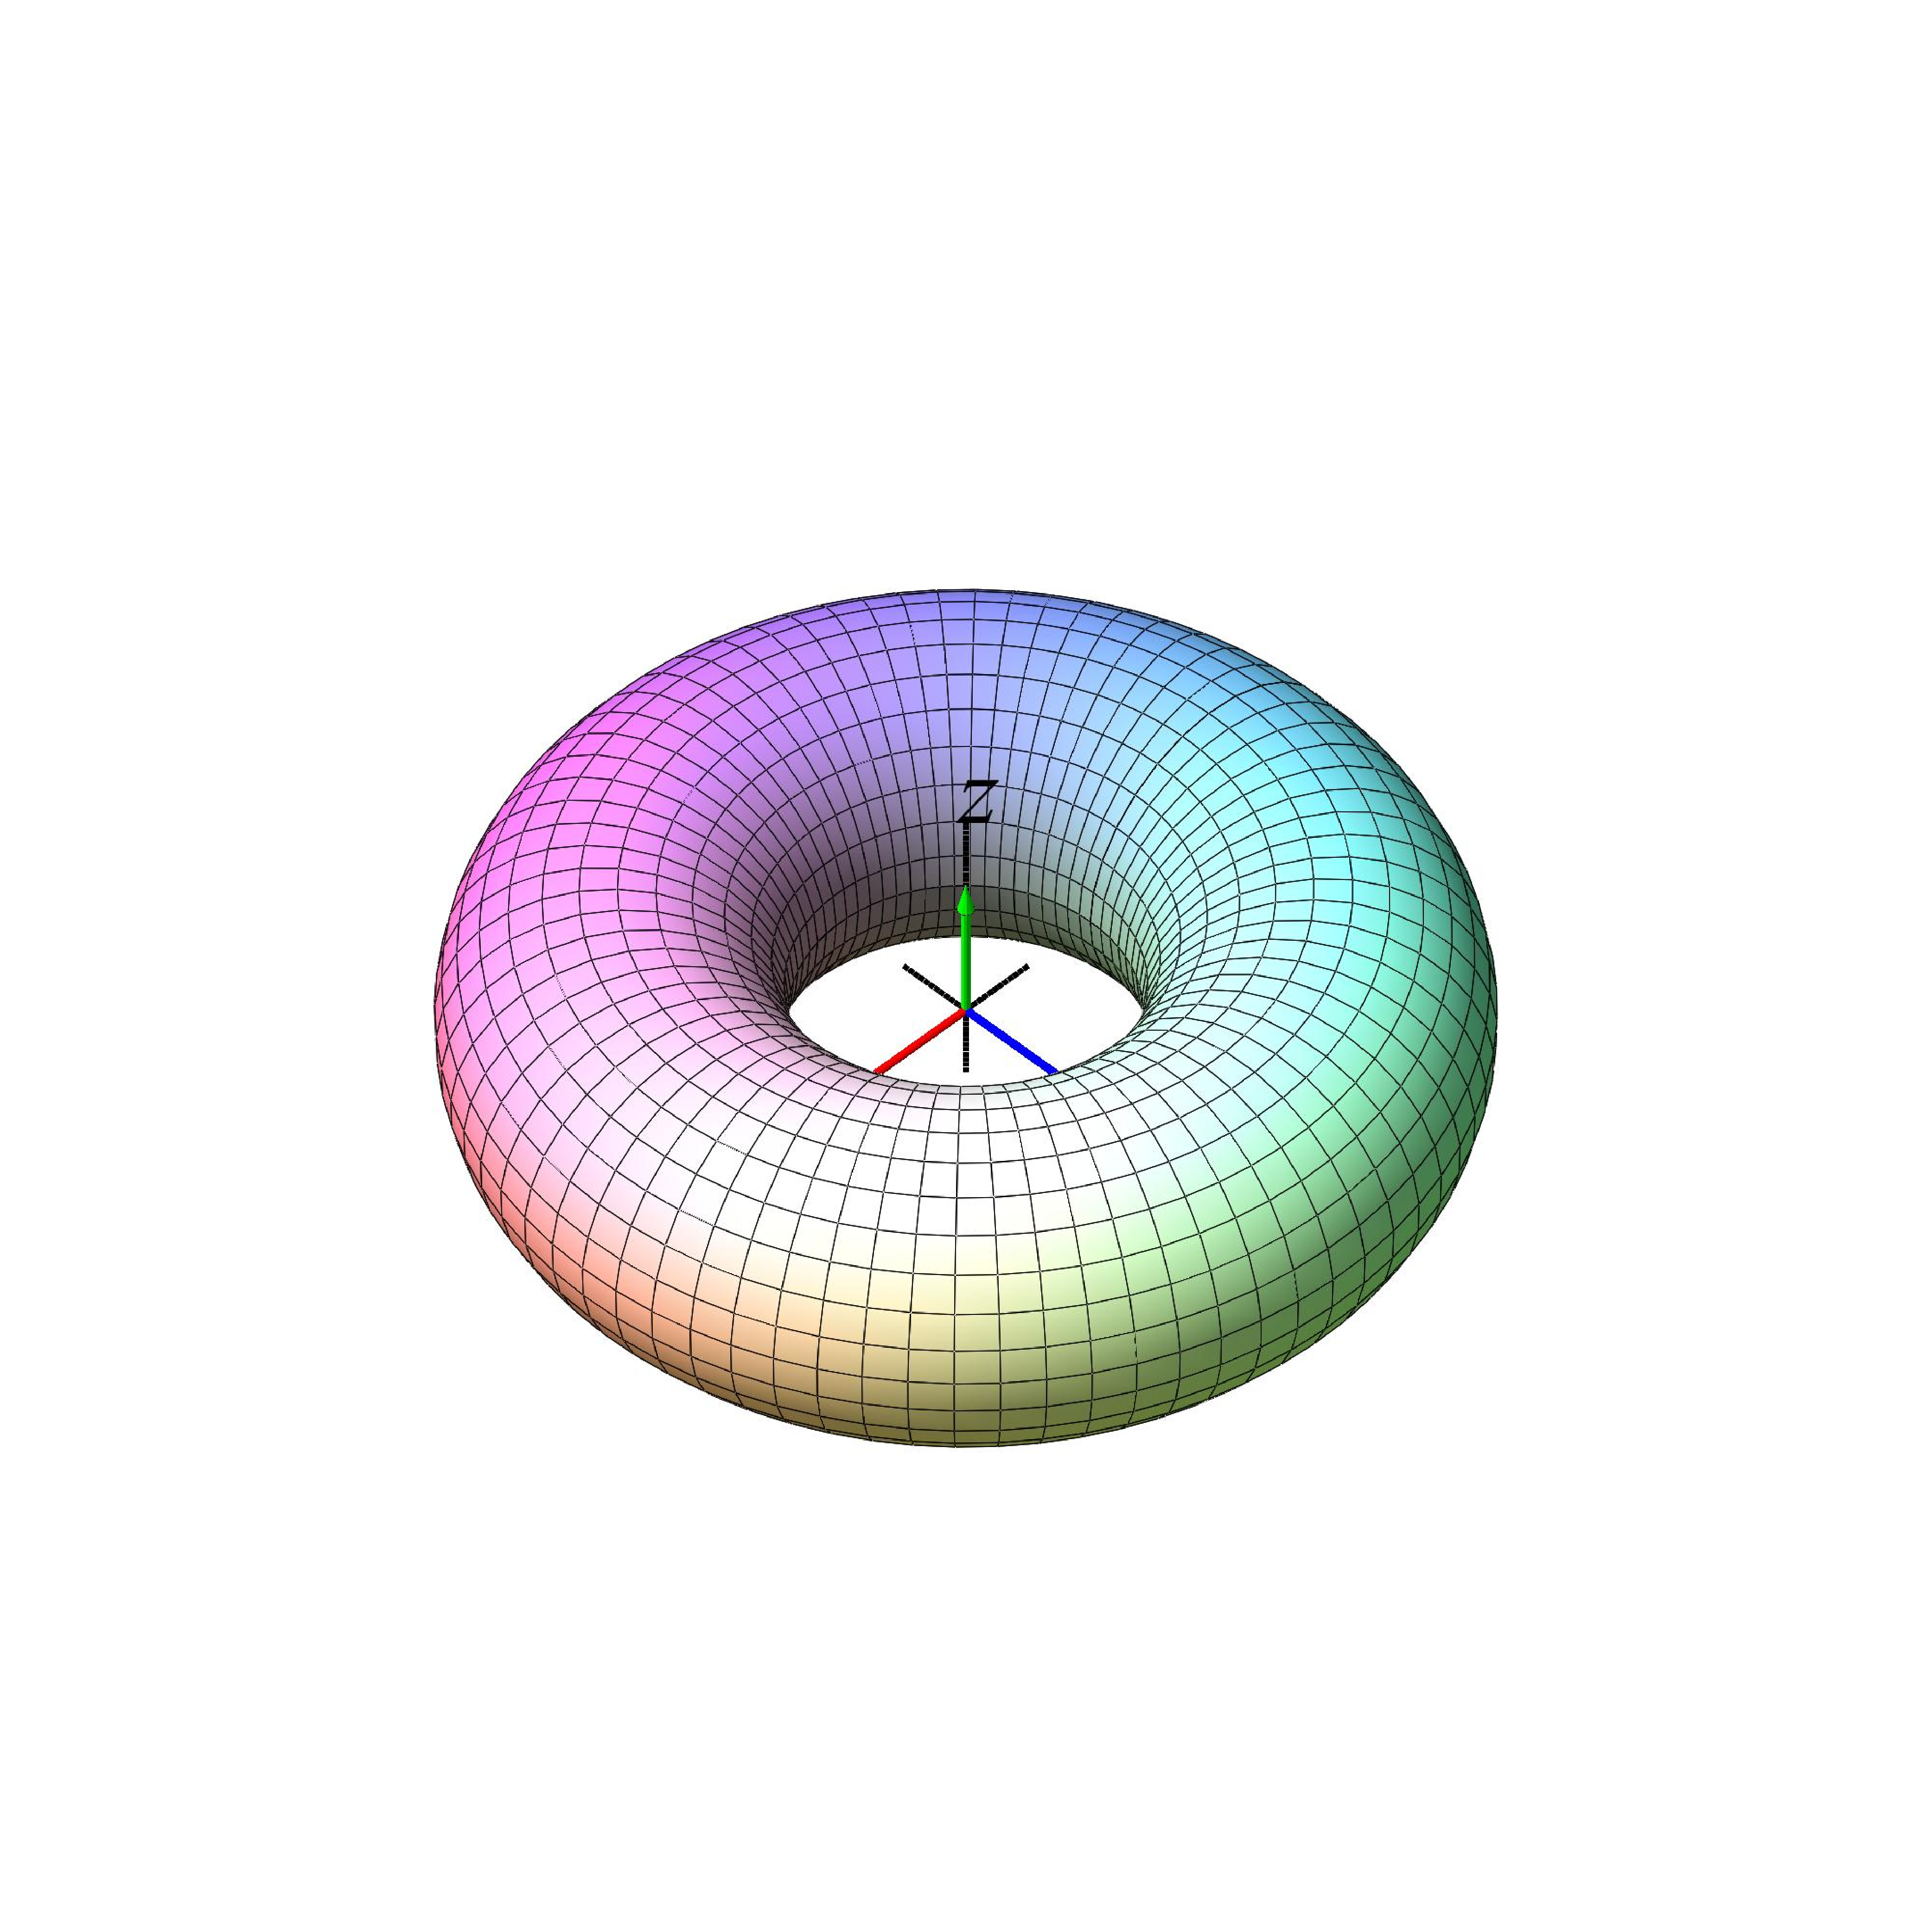
\includegraphics[height=60mm]{FIGS/plotTorus2} 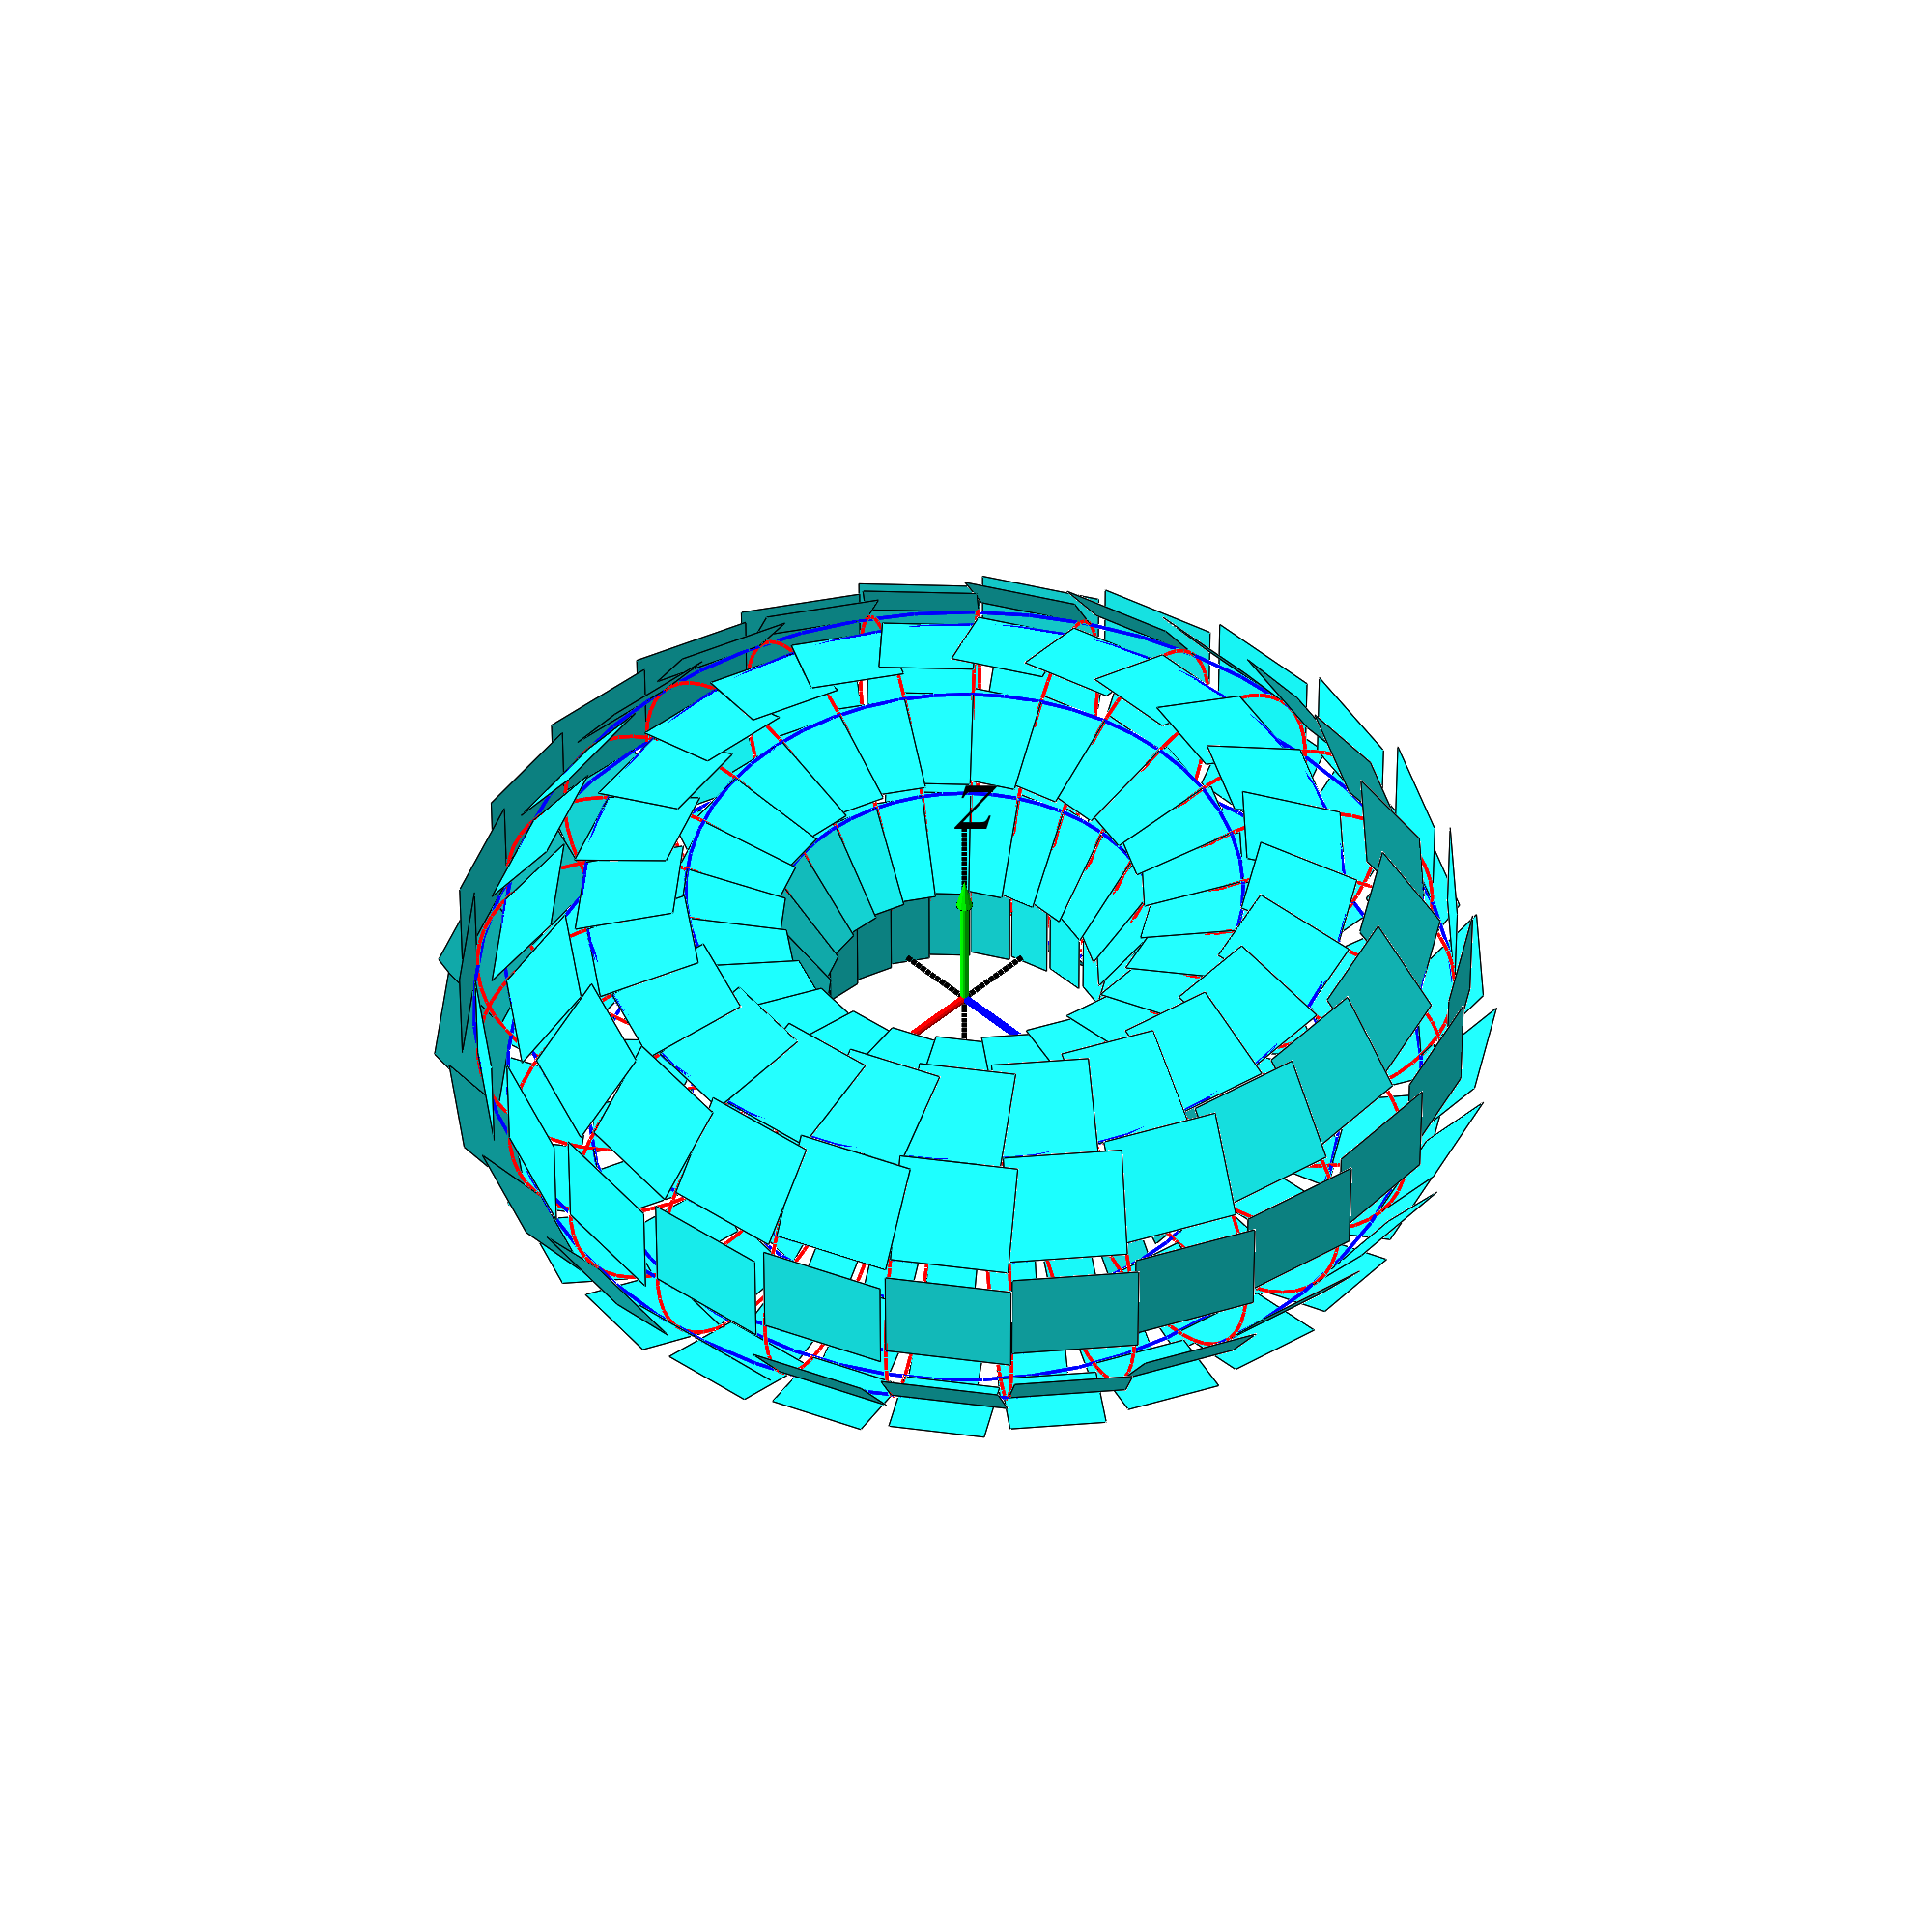
\includegraphics[height=60mm]{FIGS/plotTorus3}}
\begin{center}
\caption{\small{Denne {såkaldte torus} er omdrejningsfladen
givet ved parameterfremstillingen ${\bf r}(u, v)
\, = \, (g(u)\cos(v), g(u)\sin(v), h(u)) \,\,,
\,\, u \in [-\pi, \pi ]\,\, , \, \, v \in [-\pi,
\pi]$, hvor nu $g(u) = 2 + \cos(u)$ og $h(u) =
\sin(u)$.}} \label{figTorus12}
\end{center}
\end{figure}

\begin{exercise}
Vis, at Jacobifunktionen $\Jac_{{\bf r}}(u,v)$
for parameterfremstillingen ${\bf r}(u,v)$ for
den generelle omdrejningsflade $FG_{{\bf r}}$  i
(\ref{eqFG}) er givet ved
\begin{equation}
\Jac_{{\bf r}}(u,v)\, = \,
g(u)\,\sqrt{(h'(u))^{2} + (g'(u))^{2}} \quad .
\end{equation}
\end{exercise}



\begin{figure}[h]
\centerline{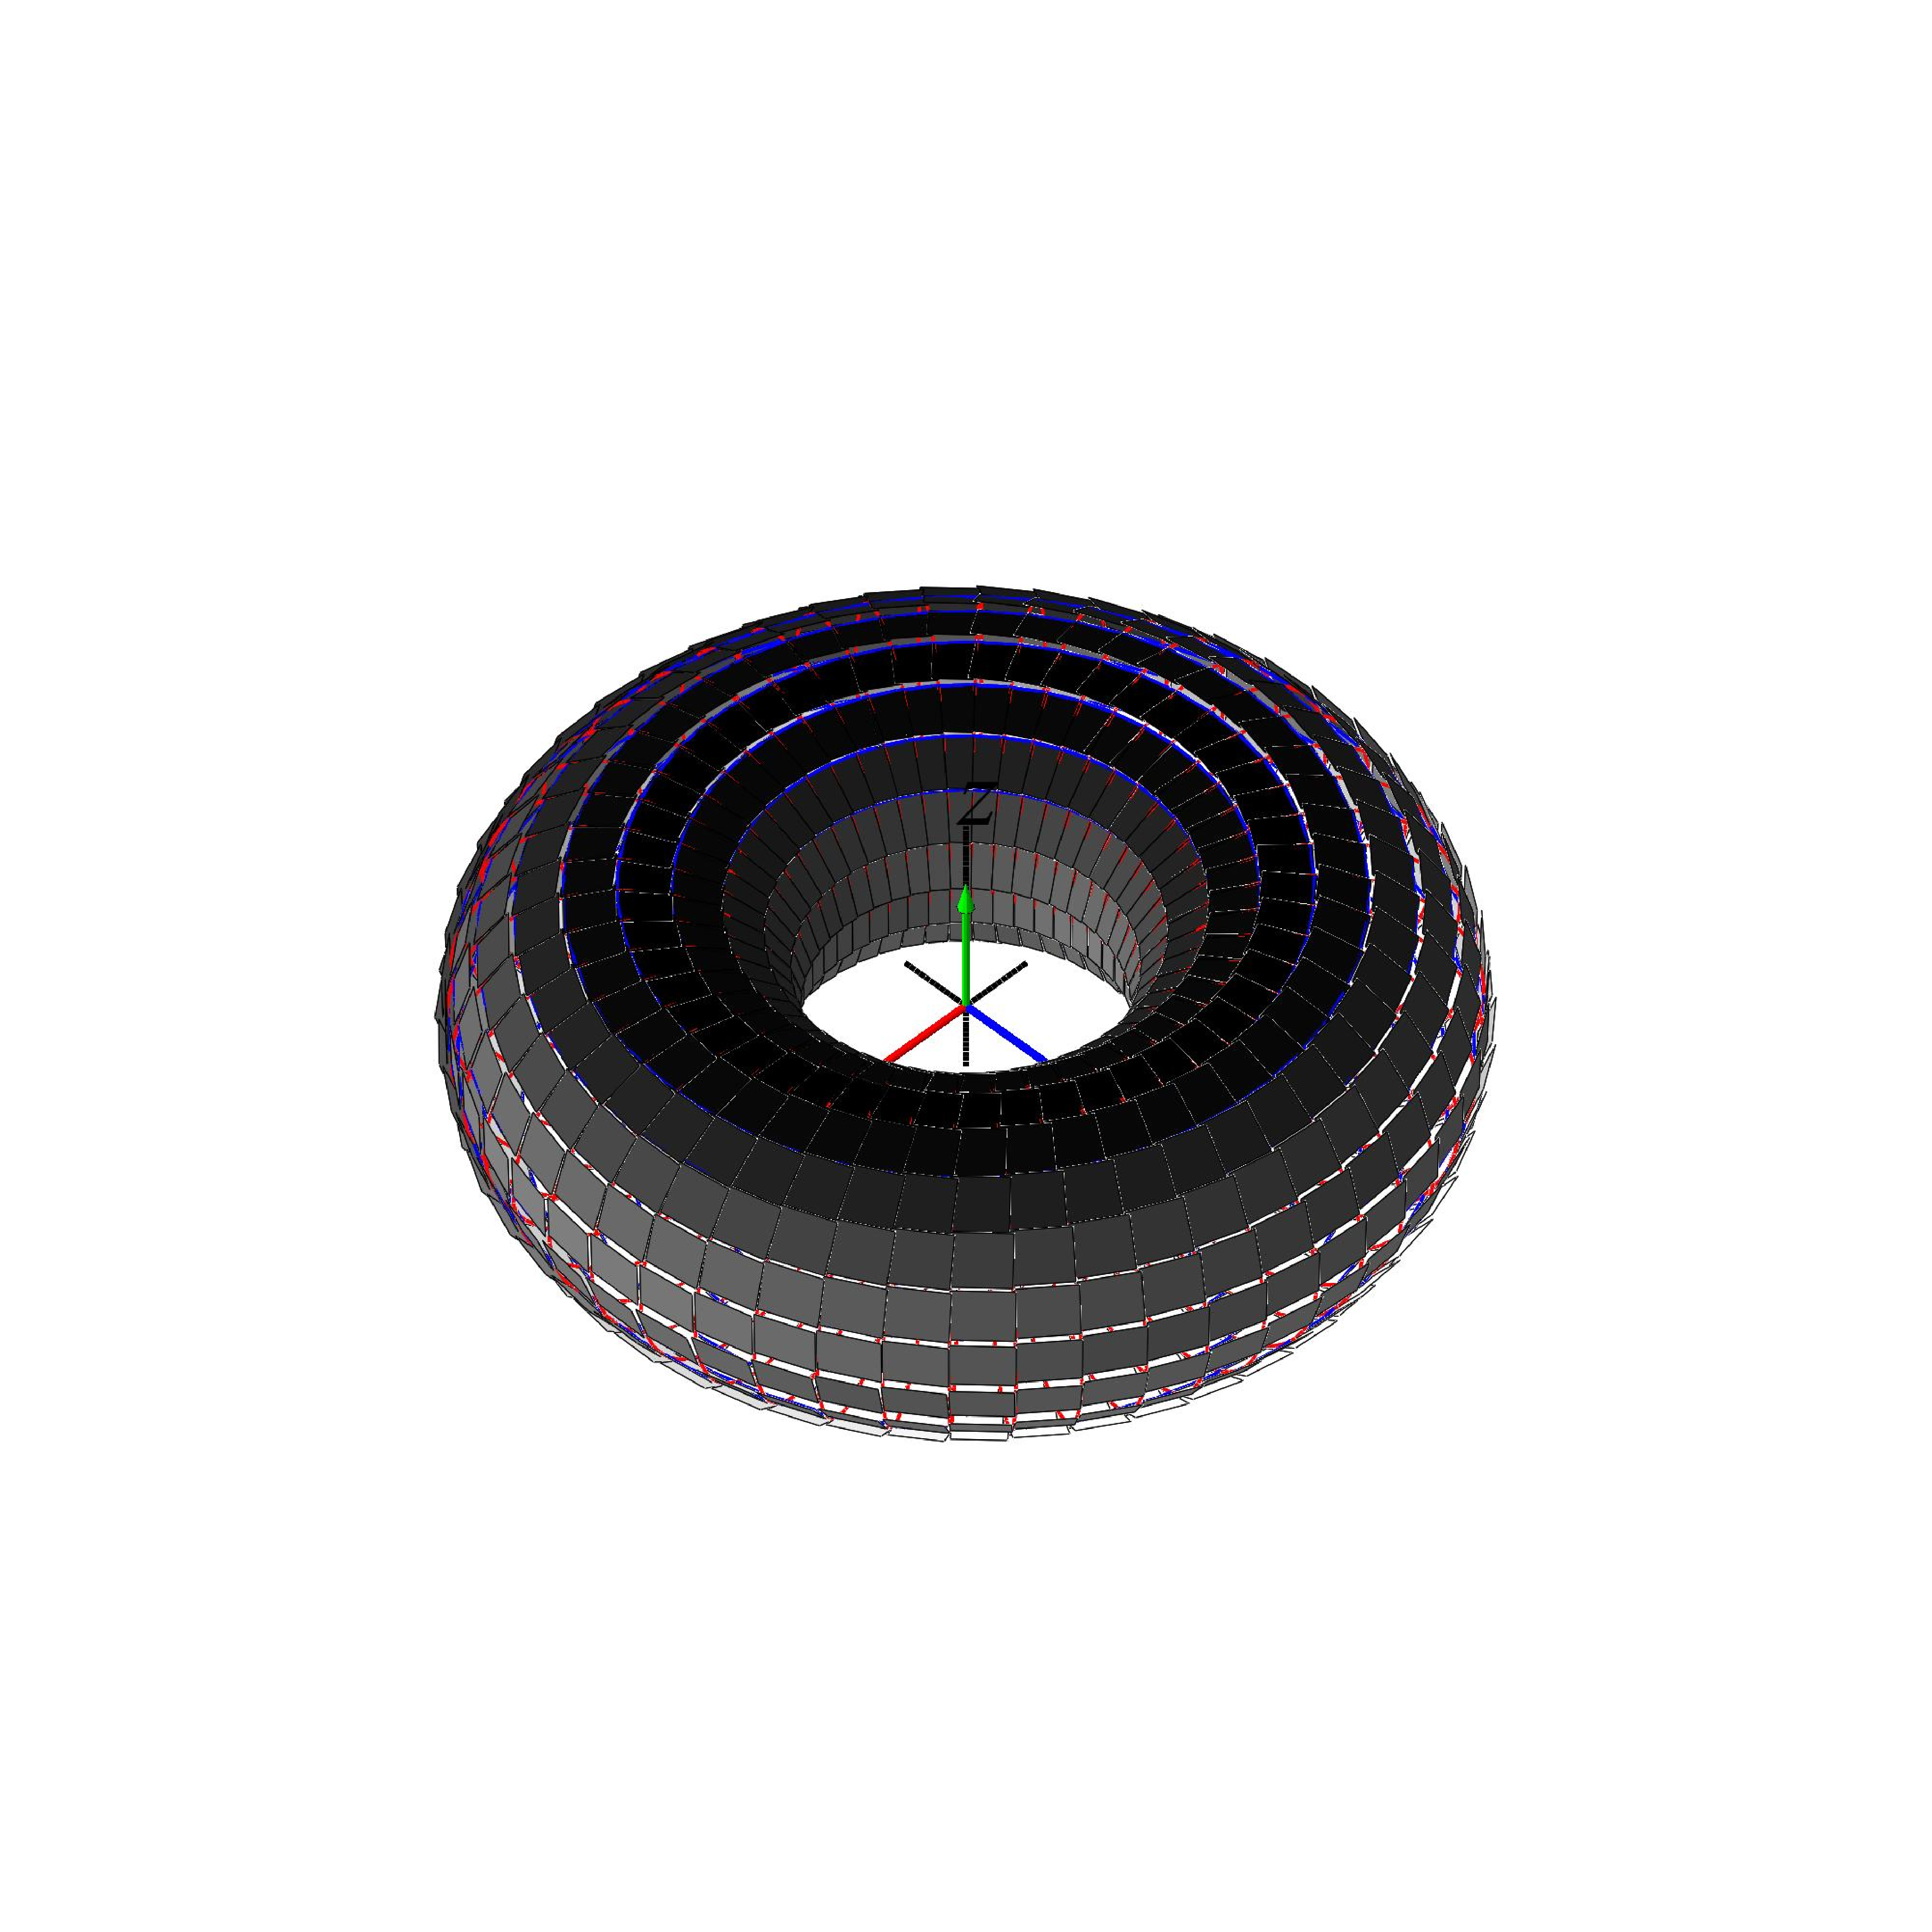
\includegraphics[height=80mm]{FIGS/plotTorusWeight3}}
\begin{center}
\caption{\small{Denne {torus} er den samme som i figur \ref{figTorus12}, men er her givet vægtfunktionen $f(x,y,z)= 2+z$. Den totale masse af den vægtede torus er $M= 16\pi^{2}$.}} \label{figTorusWeight3}
\end{center}
\end{figure}



\begin{example}[Torus-areal]\label{exampTorusArea}
En given torus er parametriseret på følgende måde:
\begin{equation}
\mathcal{T} \quad : \quad {\bf r}(u, v)
\, = \, (g(u)\cos(v), g(u)\sin(v), h(u)) \,\,,
\,\, u \in [-\pi, \pi ]\,\, , \, \, v \in [-\pi,
\pi] \quad ,
\end{equation}
hvor $g(u) = 2 + \cos(u)$ og $h(u) =
\sin(u)$. \\

Jacobifunktionen er
\begin{equation}
\Jac_{\mathbf{r}}(u,v)  = \,
g(u)\,\sqrt{(h'(u))^{2} + (g'(u))^{2}} = 2 + \cos(u) \quad,
\end{equation}
så arealet af denne torus er simpelthen:
\begin{equation}
\Ar(\mathcal{T}) = \int_{-\pi}^{\pi} \int_{-\pi}^{\pi} (2 + \cos(u))\, du \, dv = 8\pi^{2} \quad.
\end{equation}
Hvis vi 'belaster' denne torus med en vægtfunktion, massetæthed, givet ved funktionen $f(x,y,z)=2 + z$ får vi den totale vægt af torusen:
\begin{equation}
\M(\mathcal{T}) =  \int_{-\pi}^{\pi} \int_{-\pi}^{\pi} (2 + \sin(u))\cdot(2 + \cos(u))\, du \, dv = 16\pi^{2} \quad.
\end{equation}
\end{example}






%%%%%%%%%%%%%%%%%%%%%%%%%%%%%%%%%%%%%%%%%%%%%%%%%%%
%%%%%%%%%%%%%%%%%%%%%%%%%%%%%%%%%%%%%%%%%%%%%%%%%%%
%%%%%%%%%%%%%%%%%%%%%%%%%%%%%%%%%%%%%%%%%%%%%%%%%%%
%%%%%%%%%%%%%%%%%%%%%%%%%%%%%%%%%%%%%%%%%%%%%%%%%%%





\section{Rum-integraler} \label{secRumInt}


Et parametriseret {rumligt område} er på samme måde som kurver og
flader givet ved en parameterfremstilling, nu med følgende form hvor de tre koordinatfunktioner $x$, $y$, og $z$ nu er funktioner af de ialt $3$ parameter-variable $u$, $v$, og $w$:
\begin{equation}
\label{eqRumOmr}
\begin{aligned}
\Omega_{\bf r}: \quad {\bf r}(u,v,w) \, = \, &\left(x(u,v,w),
y(u,v,w), z(u,v,w)\right) \in \mathbb{R}^3 \quad , \\ \, \, \,  &u
\in [a, b] \, \, , \, \,  v \in [c,d] , \, \, \,  w \in [h,
l]\quad.
\end{aligned}
\end{equation}


\begin{definition}[Rumintegral] \label{defRumInt}
Lad $f(x,y,z)$ betegne en kontinuert funktion i $\mathbb{R}^{3}$.
Rumintegralet af funktionen $f(x,y,z)$ over det parametriserede rumlige
område $\Omega_{\bf r}$ defineres ved
\begin{equation} \label{eqRumintegral}
\int_{\Omega_{\bf r}} f \, d\mu \, = \, \int_{h}^{l}\int_{c}^{d}
\int_{a}^{b} f({\bf r}(u,v,w))\, \Jac_{\bf r}(u,v,w)\, du \, dv \,
dw \quad,
\end{equation}
hvor {Jacobi-funktionen $\Jac_{\bf r}(u,v,w)$} nu er givet ved
\begin{equation}
\begin{aligned}
 \Jac_{\bf r}(u,v,w)\, = \, | \,({\bf r}'_{u}(u,v,w)\times{\bf
 r}'_{v}(u,v,w))\cdot{\bf r}'_{w}(u,v,w)\, |
         \quad .
 \end{aligned}
\end{equation}
Det vil sige, $\Jac_{\bf r}(u,v,w)$ er volumenet (her beregnet som et rumprodukt) af
det parallelepipedum, der på stedet ${\bf
r}(u,v,w)$ udspændes af de tre
koordinatkurve-tangentvektorer ${\bf
r}'_{u}(u,v,w)$ , ${\bf
 r}'_{v}(u,v,w)$ og ${\bf
r}'_{w}(u,v,w)$.
\end{definition}

\begin{exercise}
Vis, at Jacobifunktionen $\Jac_{\bf r}(u,v,w)$ også kan findes som den numeriske
værdi af determinanten af den matrix, der som søjler har
koordinaterne for de tre vektorer ${\bf r}'_{u}(u,v,w)$, ${\bf
r}'_{v}(u,v,w)$ og ${\bf r}'_{w}(u,v,w)$.
\end{exercise}

\begin{definition}[Regulær parameterfremstilling] \label{defReParamSpatial}
Parameterfremstillingen i (\ref{eqRumOmr}) kaldes en {\em{{regulær parameterfremstilling}}} hvis
$\, \Jac_{\bf r}(u,v,w)\, > \, 0\,$ for alle $\, u
\in [a, b] \, \, , \, \,  v \in [c,d] , \, \, \,  w \in [h,
l]\, $.
\end{definition}

\begin{definition}[En-entydig parameterfremstilling] \label{defEnEntydSpatial}
Som for kurver og flader vil vi kalde parameterfremstillingen i
(\ref{eqRumOmr}) {en-entydig} hvis forskellige punkter i
definitionsmængden afbildes i forskellige punkter i billedmængden.
\end{definition}



\begin{definition}[Rumfang, volumen] \label{defRumfang}
{Volumenet} eller {rumfanget} af det rumlige område
\begin{equation}
\Omega_{\bf r}: \quad {\bf r}(u,v,w) \, = \, \left(x(u,v,w),
y(u,v,w), z(u,v,w)\right) \quad ,
\end{equation}
hvor
\begin{equation}
u \in [a, b] \quad , \quad
 v \in [c,d] \quad ,\quad \textrm{og} \quad  w \in [h, l] \quad ,
\end{equation}
defineres som
rumintegralet af den konstante funktion $1$:
\begin{equation} \label{eqRumintegralVolumen}
\Vol(\Omega_{\bf r}) \, = \, \int_{\Omega_{\bf r}} 1 \, d\mu \, =
\, \int_{h}^{l}\int_{c}^{d} \int_{a}^{b} \Jac_{\bf r}(u,v,w)\,du
\, dv \, dw \quad .
\end{equation}
\end{definition}


\begin{figure}[h]
\centerline{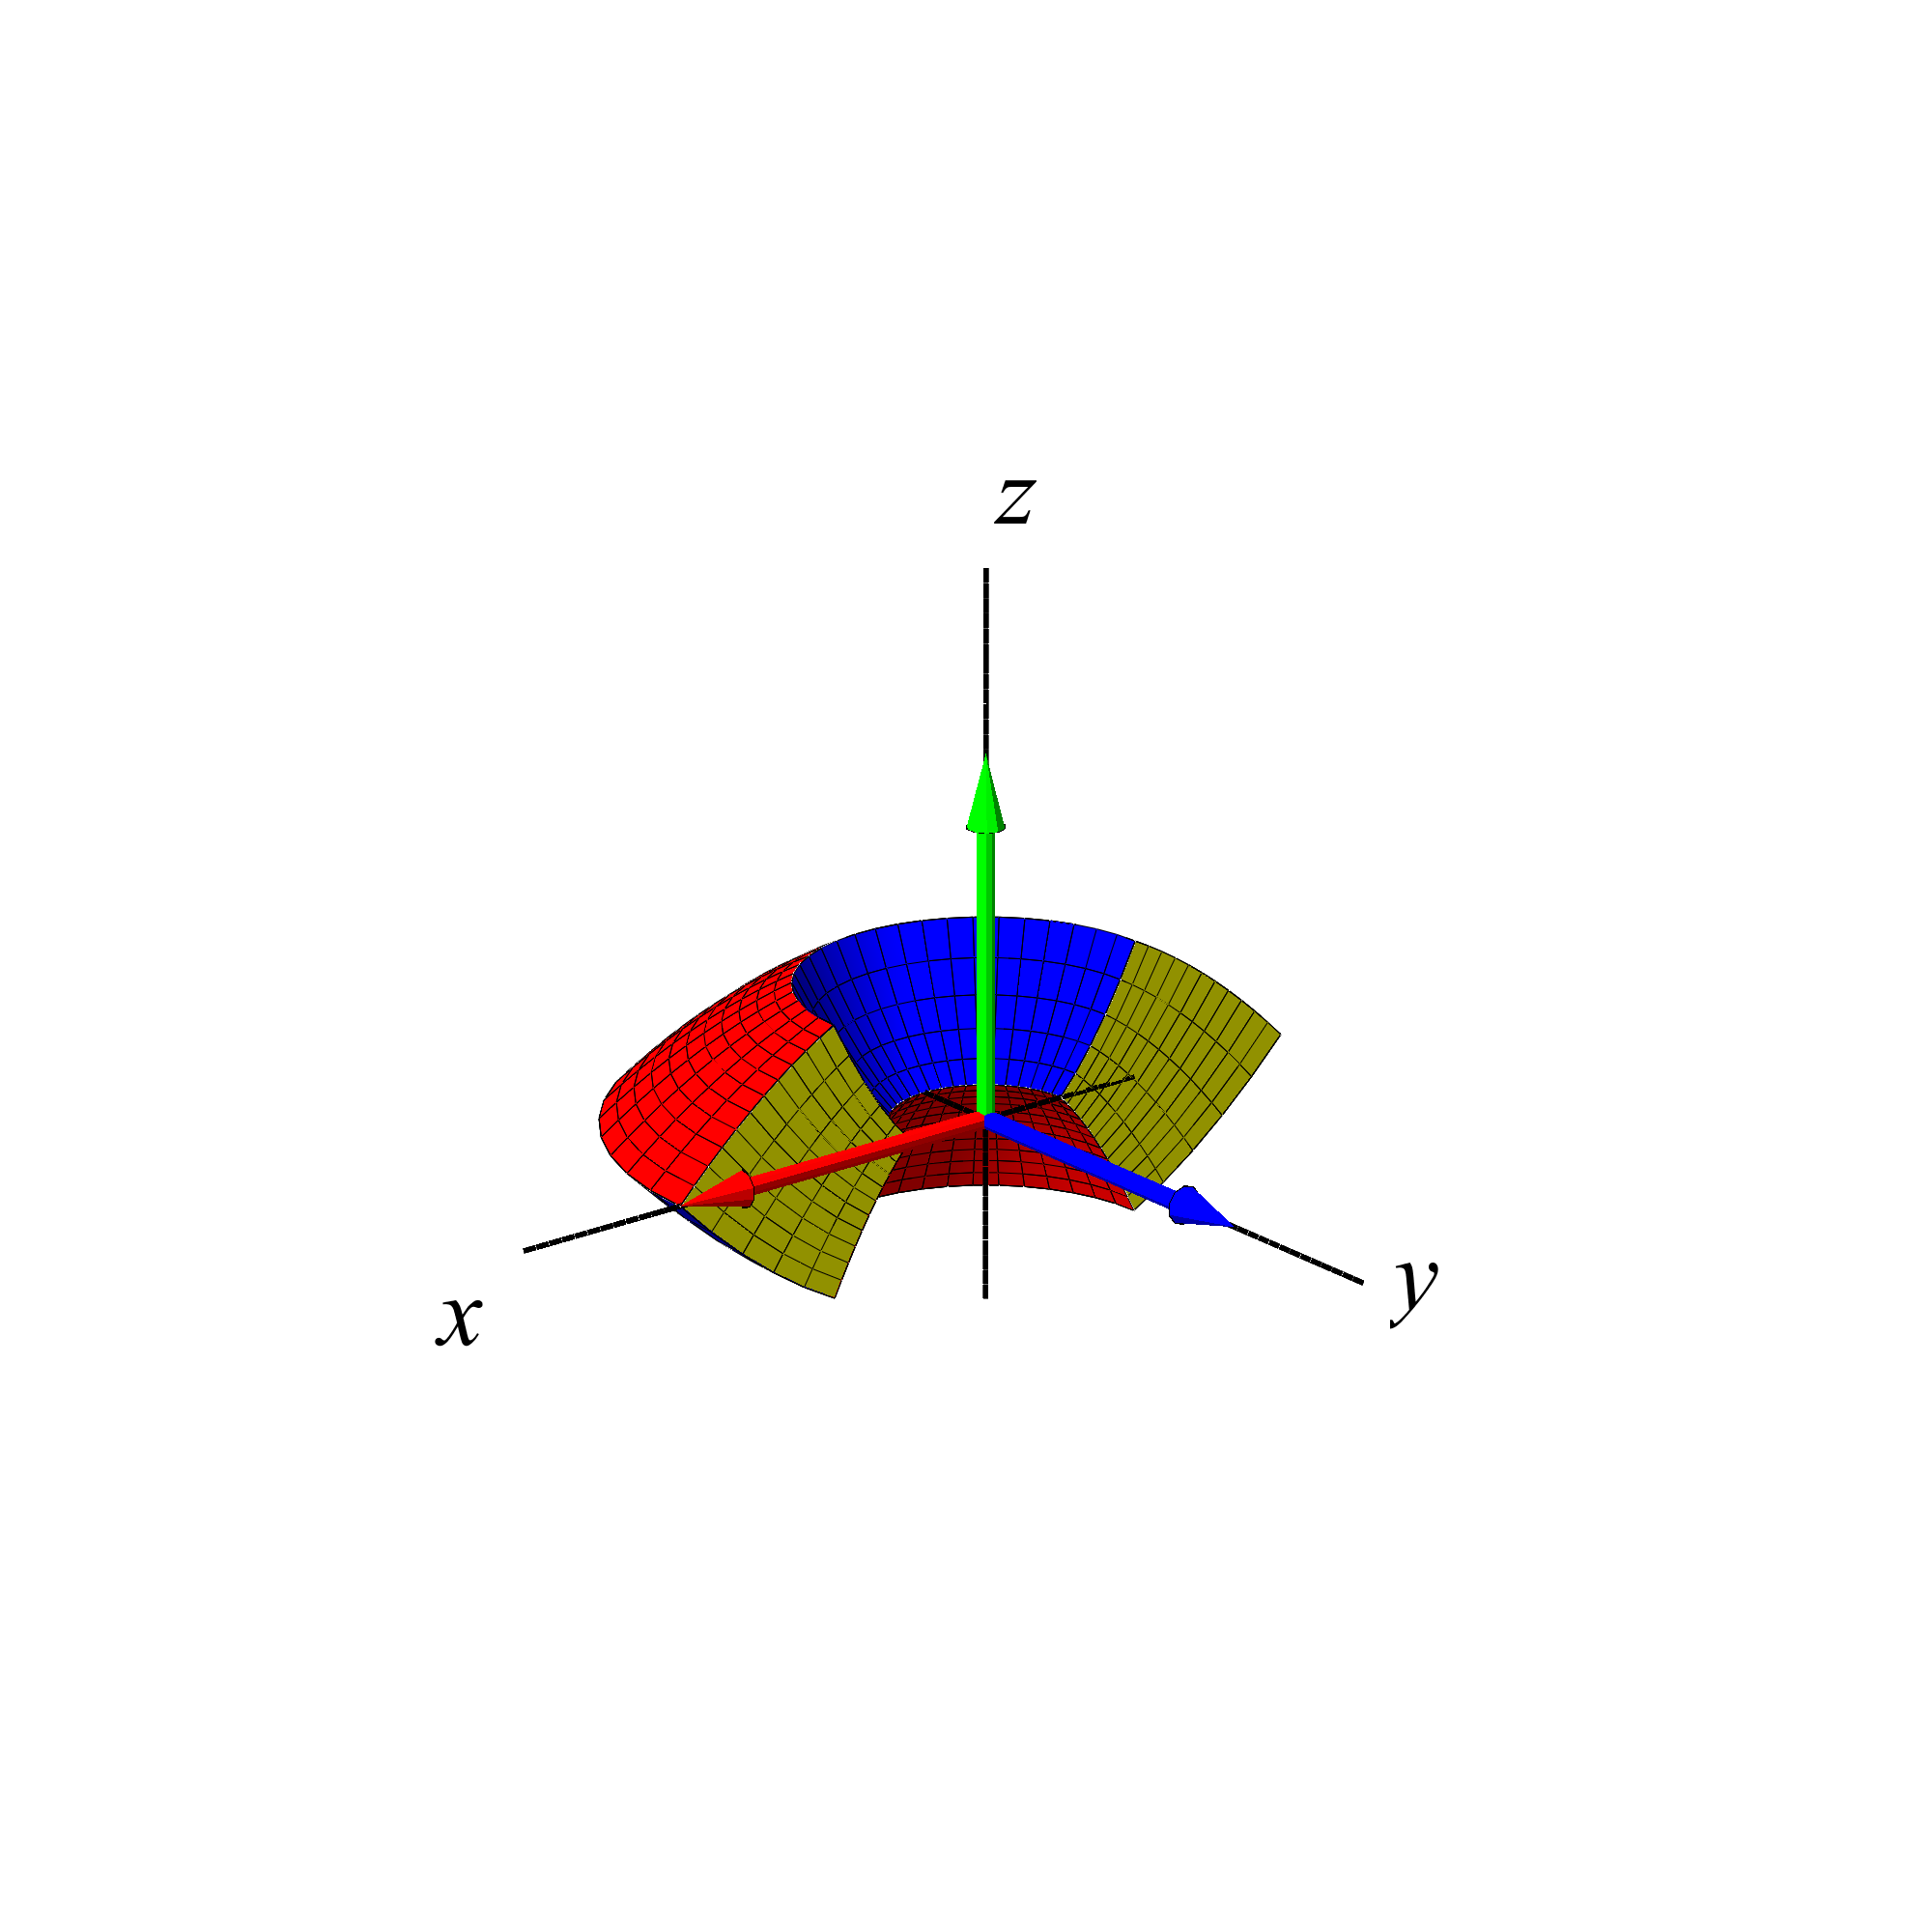
\includegraphics[height=60mm]{FIGS/plotParab3D1}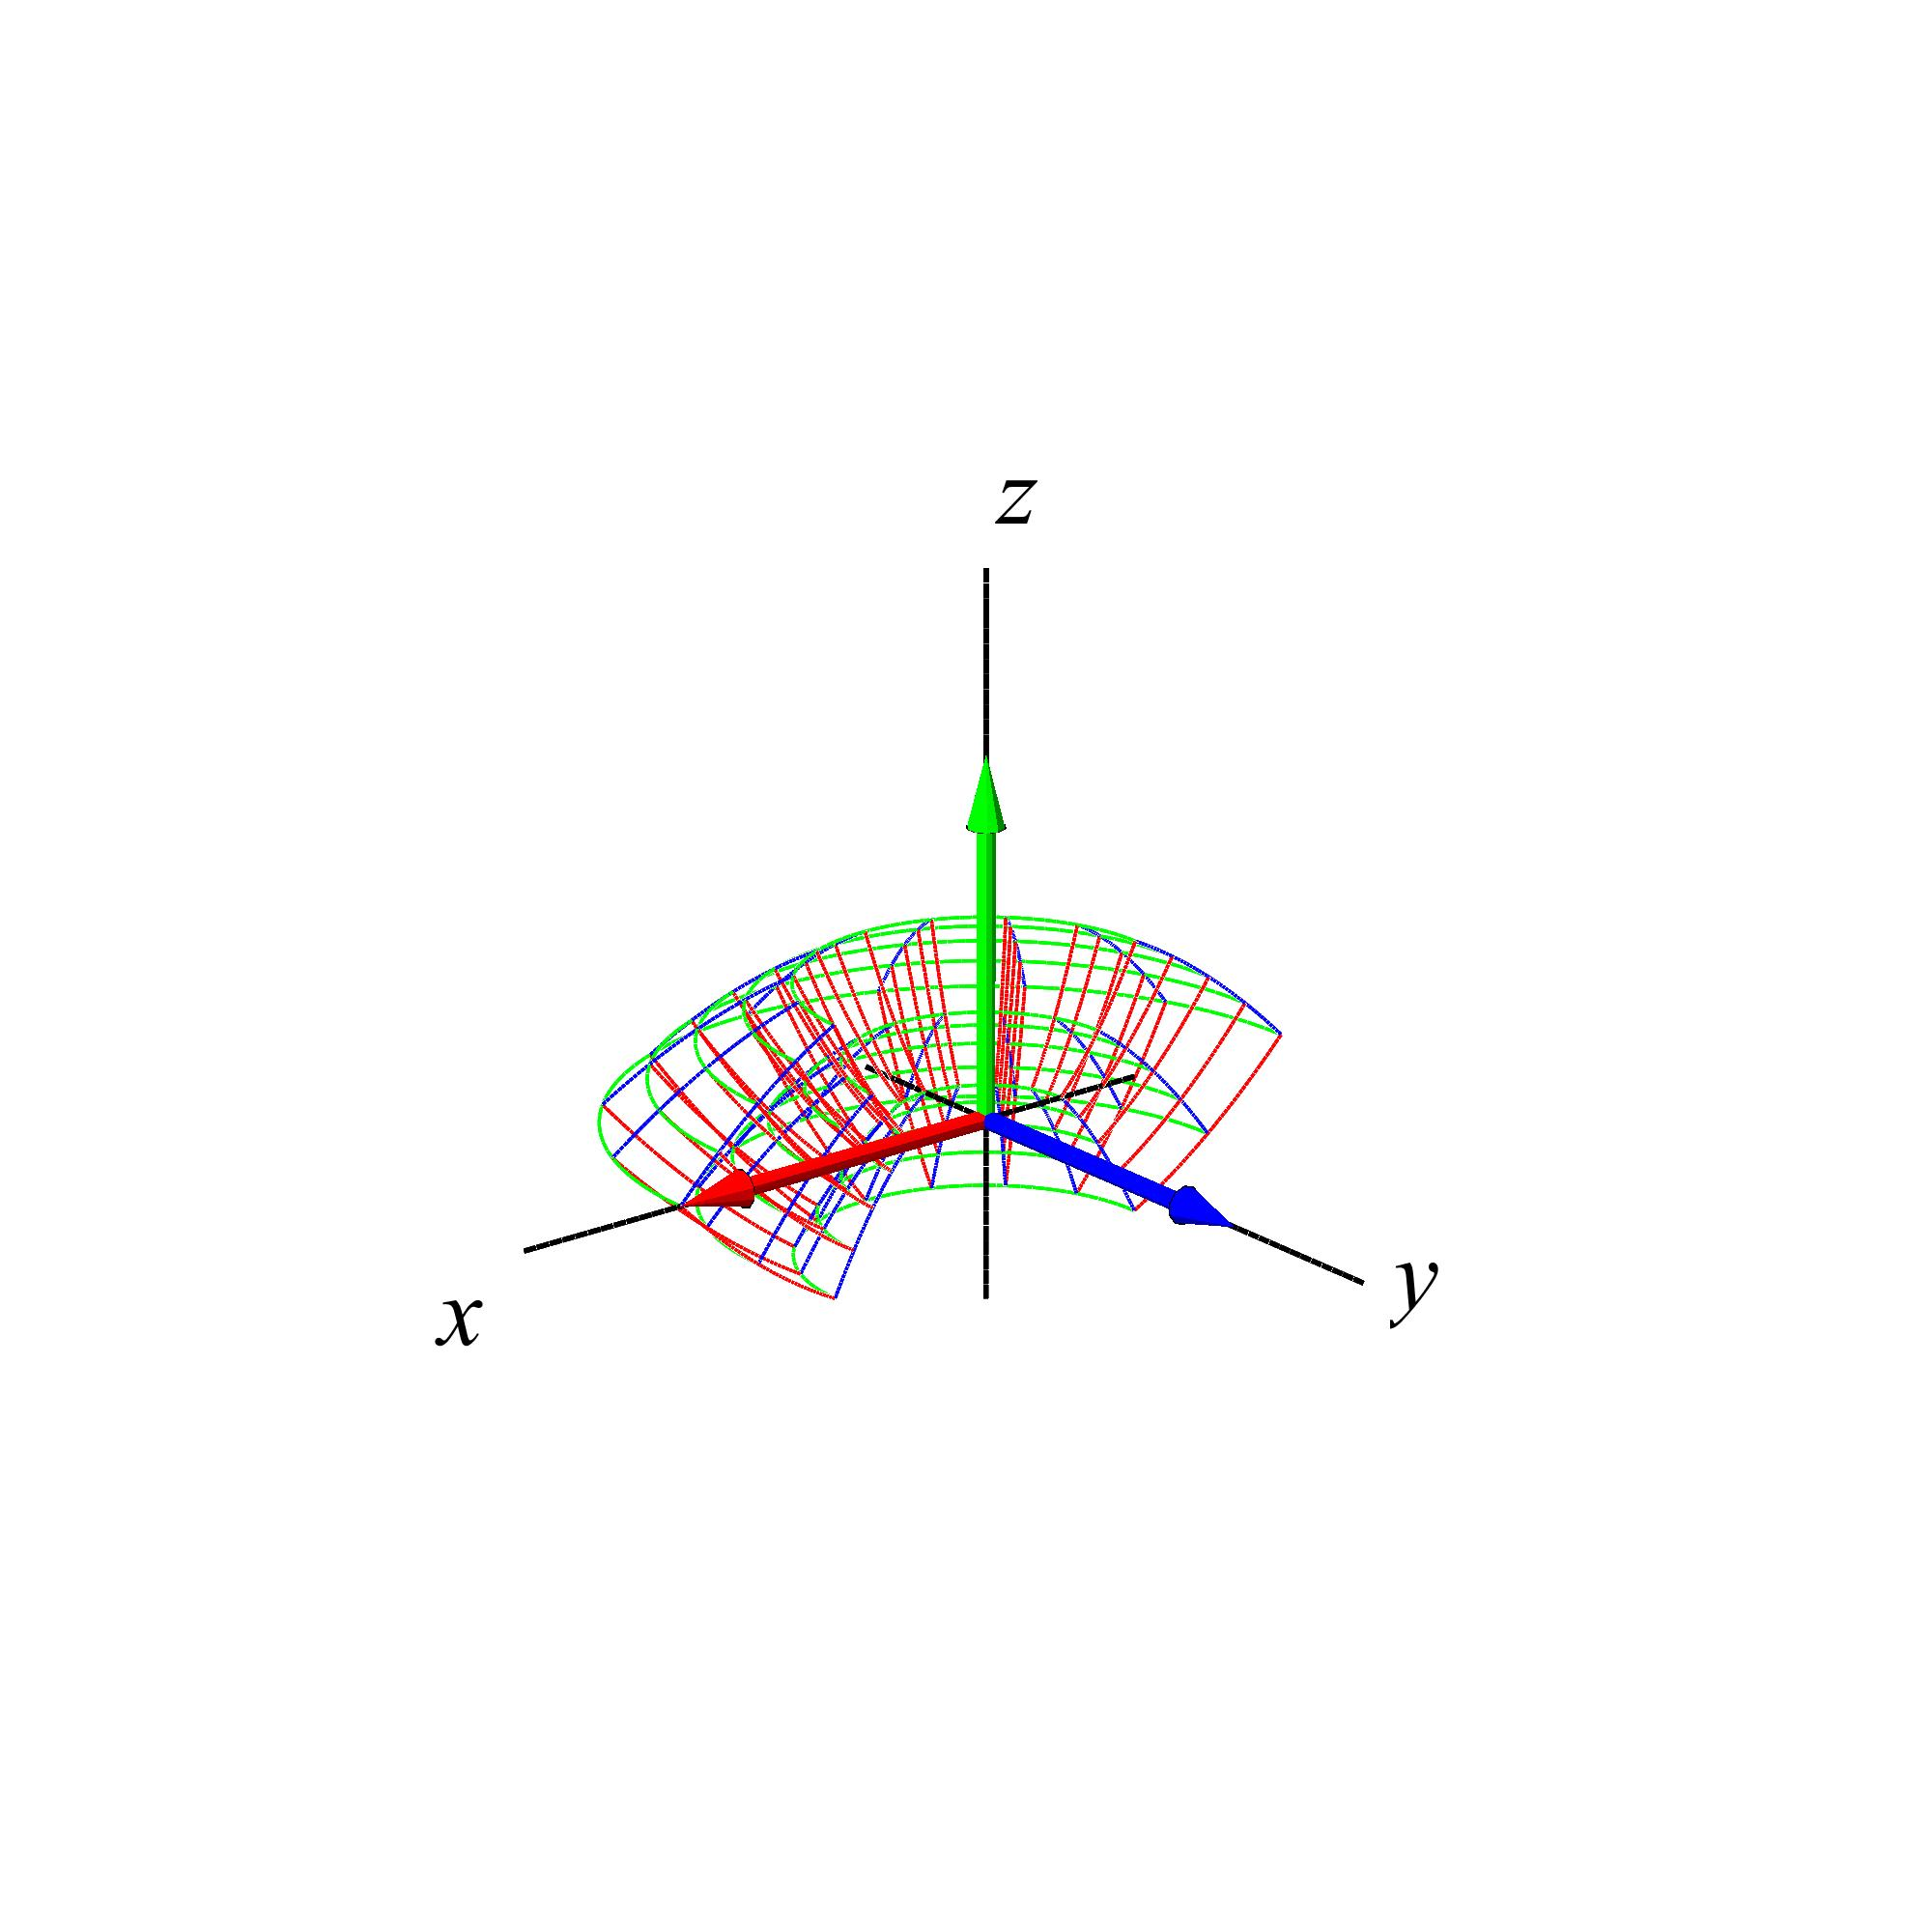
\includegraphics[height=60mm]{FIGS/plotParab3D2}  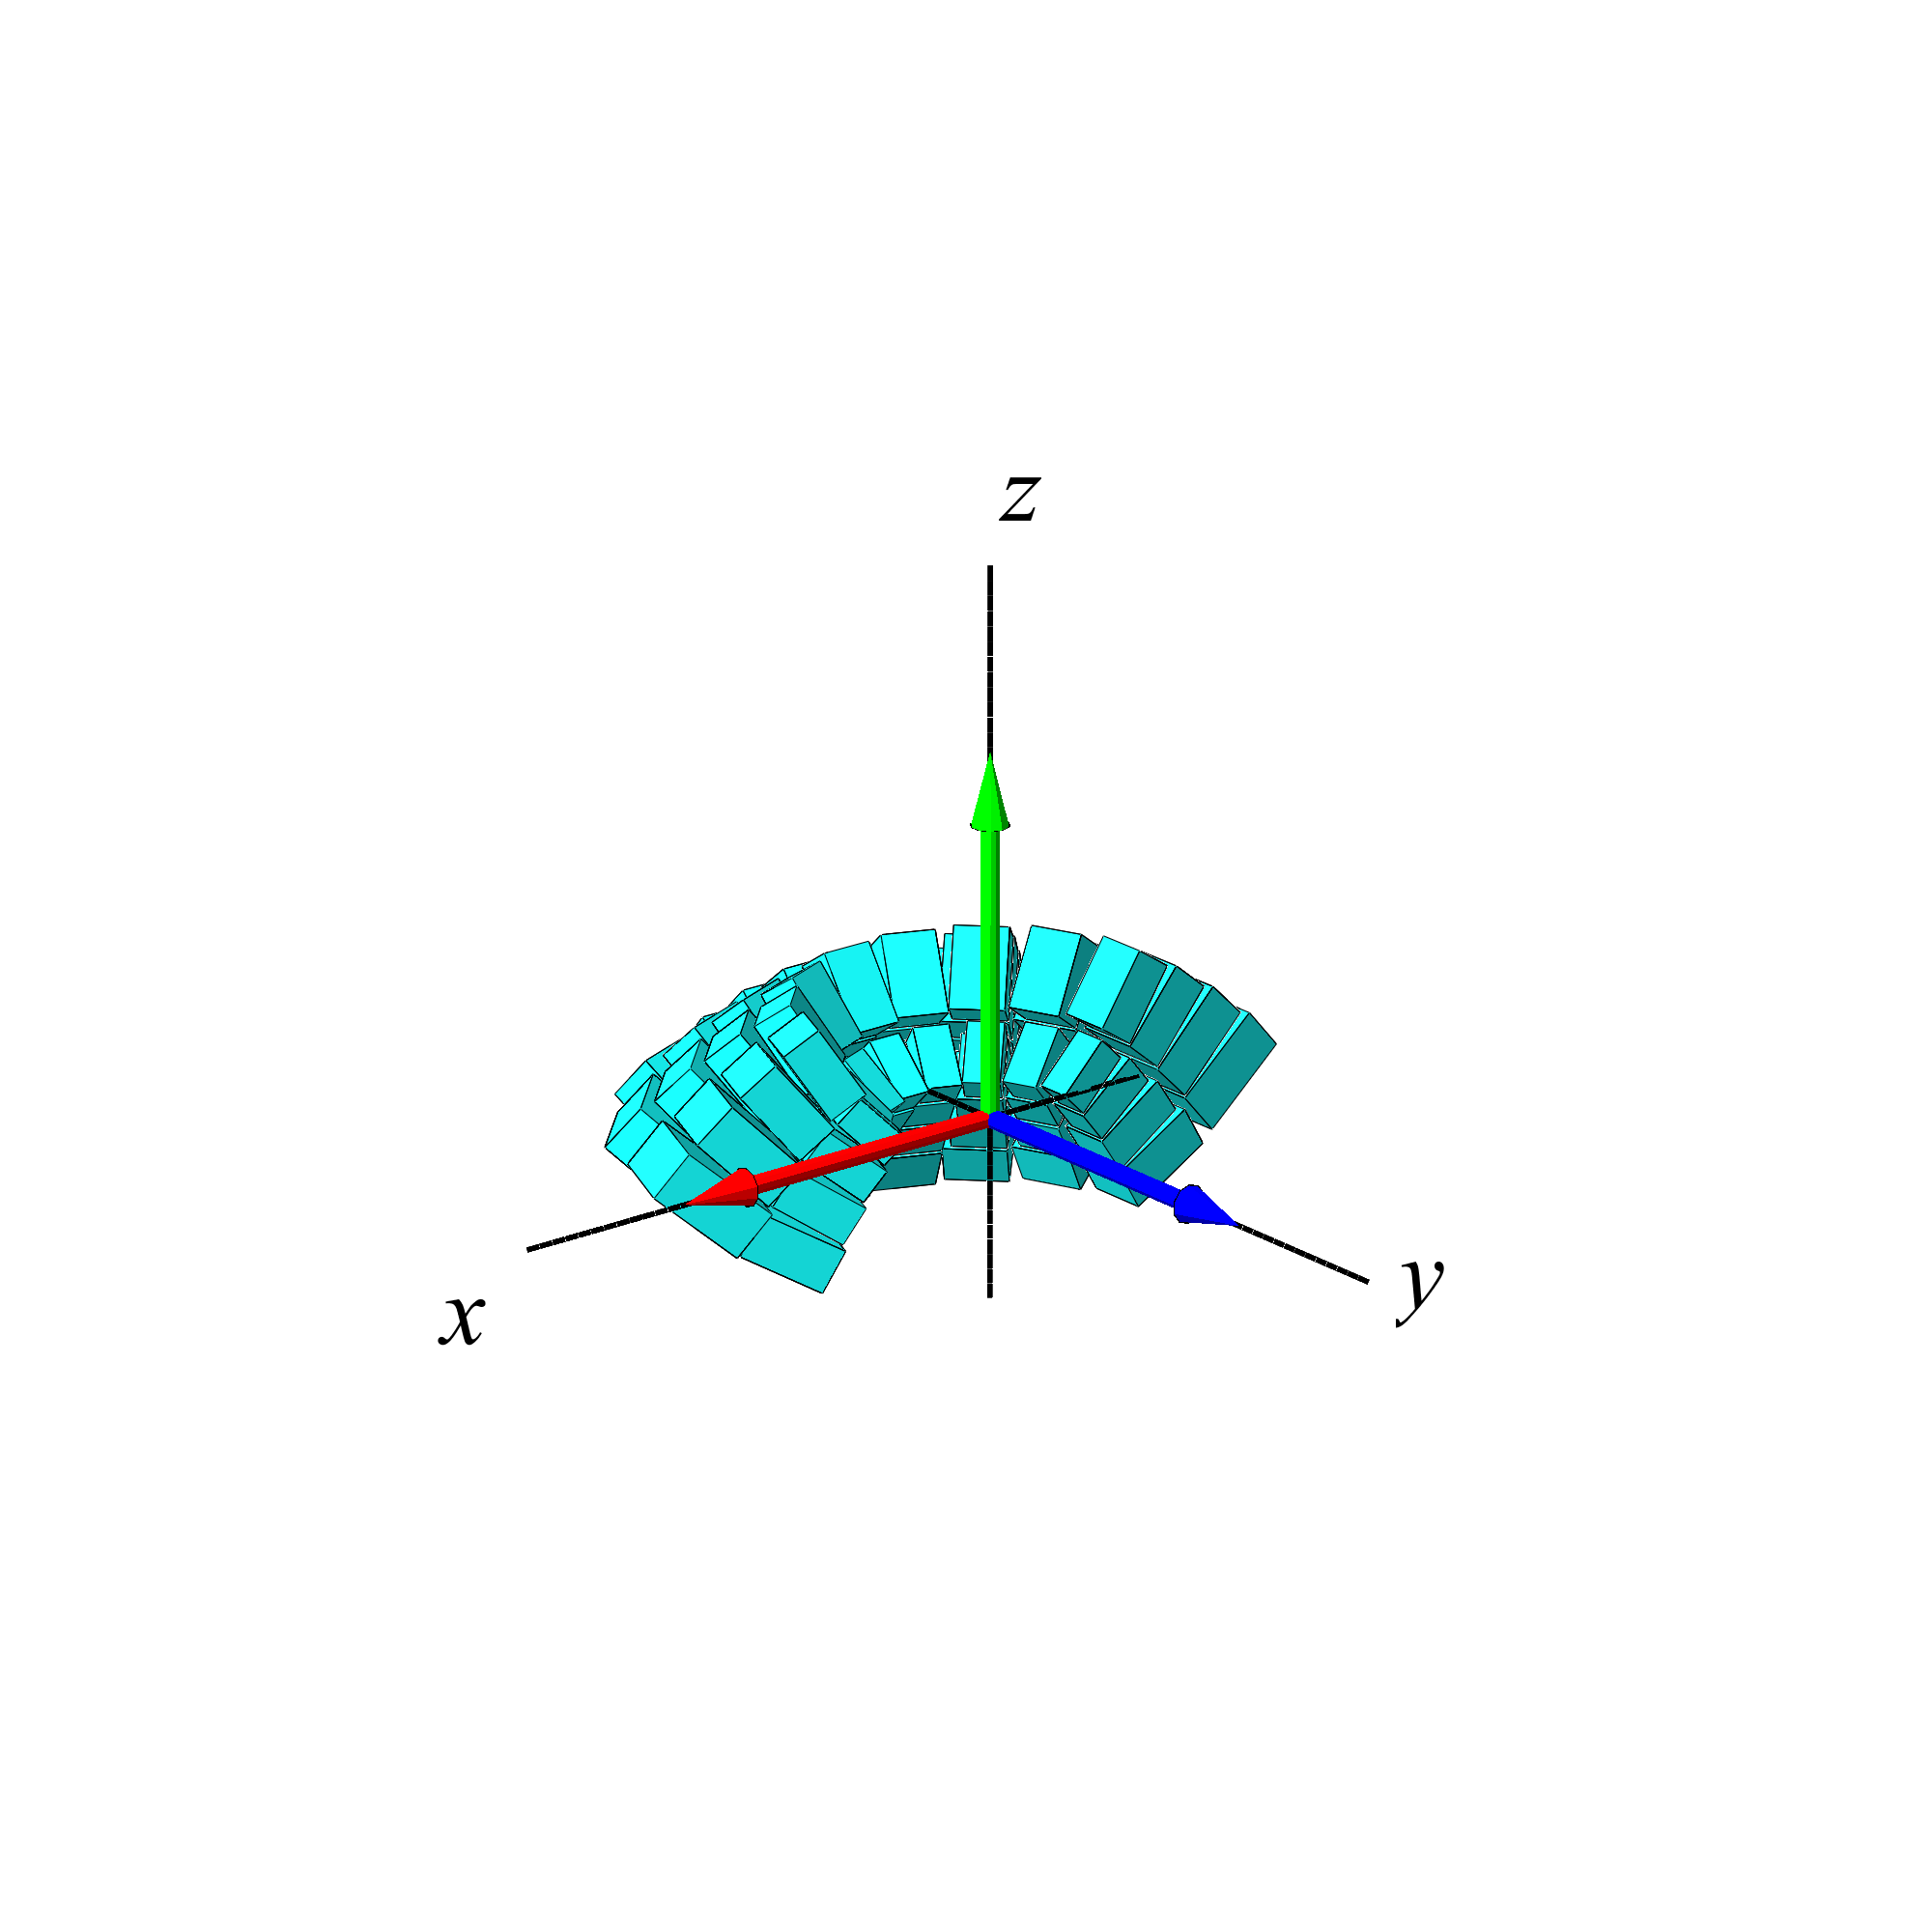
\includegraphics[height=60mm]{FIGS/plotParab3D3}}
\begin{center}
\caption{\small{Billeder af det rumlige område
givet ved parameterfremstillingen ${\bf r}(u, v,
w) \, = \, (u\,v\cos(w), u\,v\sin(w),
\frac{1}{2}(u^2 - v^2) ) \,\,, \,\, u \in
[\frac{1}{2}, 1 ]\,\, , \, \, v \in [\frac{1}{2},
1]\,\, , \, \, w \in [\pi, 2\pi] $.}} \label{fig3d13}
\end{center}
\end{figure}

\begin{exercise}
Vis, at parameterfremstillingen i figur \ref{fig3d13} er regulær og
en-entydig.
\end{exercise}



%%%%%%%%%%%%%%%%%%%%%%%%%%%%%%%%%%%%%%%%%%%%%%%%%%%
%%%%%%%%%%%%%%%%%%%%%%%%%%%%%%%%%%%%%%%%%%%%%%%%%%%





\subsection{Motivering af rumintegralet}\label{subsecMotivRum}
Intervallerne $[a, b]$,
 $[c, d]$ og  $[h,l]$ inddeles i henholdsvis $n$, $m$ og $q$
lige store dele. Så har hvert $u$-delinterval længden $\delta_{u} \,
= \, (b-a)/n$, hvert $v$-delinterval har længden $\delta_{v} \, = \,
(d-c)/m$ og hvert $w$-interval har længden $\delta_{w} \, = \,
(l-h)/q$. Tilsvarende bliver delepunkternes koordinater i $(u, v,
w)$-parameterområdet (som her er det retvinklede 'kasse-område'
$[a,b]\times[c,d]\times[h, k]$ i $\mathbb{R}^{3}$.


\begin{equation}
\begin{aligned}
(u_{1}, v_{1}, w_{1}) \, &= \, (a, c, h), \\
&.... \\
(u_{i}, v_{j}, w_{k}) \, &= \,
(a + (i-1)\delta_{u}, c + (j-1)\delta_{v}, h + (k-1)\delta_{w}), \\
 &.... \\
(b, d, l) \, &= \, (a + n\delta_{u}, c + m\delta_{v}, h +
q\delta_{w}) \quad .
\end{aligned}
\end{equation}

Med hvert af disse faste punkter $(u_{i}, v_{j}, w_{k})$ som udviklingspunkt kan vi igen
bruge Taylors grænseformel for hver af de 3 koordinat-funktioner for $${\bf r}(u,
v, w) \, = \, \left(x(u,v,w), y(u,v,w), z(u,v,w)\right)$$ til første orden og med tilhørende
epsilon-funktioner:
\begin{equation} \label{eqTaylor3}
\begin{aligned}
{\bf {r}}(u, v, w) \, = \, {\bf r}(& u_{i}, v_{j}, w_{k}) \\
+ \, &{\bf r}'_{u}(u_{i}, v_{j}, w_{k})\cdot(u-u_{i}) \\
+ \, &{\bf r}'_{v}(u_{i}, v_{j}, w_{k})\cdot(v-v_{j})  \\
+ \, &{\bf r}'_{w}(u_{i}, v_{j}, w_{k})\cdot(w-w_{k}) \\
+ \, & \rho_{ijk}\cdot{\bm{\varepsilon}}_{ijk}(u-u_{i}, v-v_{j},
w-w_{k}) \quad ,
\end{aligned}
\end{equation}
hvor $\, u\, \, \in\, \left[\, u_{i}\, , \,  u_{i} +
\delta_{u}\,\right]\, , \,\, v\, \, \in\, \left[\, v_{j}\, , \,
v_{j} + \delta_{v}\,\right]\, , \,\, w\, \, \in\, \left[\, w_{j}\, ,
\, w_{j} + \delta_{w}\,\right]\,$. Afstanden mellem det variable
punkt $\,(u\,,v\,, w)\,$ og det faste punkt $\,(u_{i}\,,v_{j}\,,
w_{k})\,$ i parameterområdet betegnes med $\,\rho_{ijk}\,$ og vi har
som før $\,{\bm{\varepsilon}}_{ijk}(u-u_{i}, v-v_{j}, w-w_{k}) \to
\, {\bf{0}}\, $ for $\, (u-u_{i}, v-v_{j}, w-w_{k}) \to (0, 0, 0)
\,$ .


Hvert parameter-delområde eller delkasse $[u_{i},
u_{i}+\delta_{u}]\times[v_{j}, v_{j}+\delta_{v}]\times[w_{k}, w_{k}
+ \delta_{w}]$ afbildes på det rumlige billed-område  ${\bf
r}(u,v,w)$, $u \in[u_{i}, u_{i}+\delta_{u}], v \in[v_{j},
v_{j}+\delta_{v}], w \in[w_{k}, w_{k}+\delta_{w}]$ i billedrummet og
dette område kan vi approksimere med den lineære del af udtrykket i
(\ref{eqTaylor3}), som fås ved at fjerne
${\bm{\varepsilon}}_{ijk}$-bidraget fra højre side i
(\ref{eqTaylor3}):
\begin{equation}\label{eqApp3}
\begin{aligned}
{\bf r}_{\app_{\,ijk}}(u, v,w) \, = \, {\bf r}(&u_{i}, v_{j}, w_{k}) \\
+ \, &{\bf r}'_{u}(u_{i}, v_{j}, w_{k})\cdot(u-u_{i}) \\+ \, &{\bf
r}'_{v}(u_{i}, v_{j}, w_{k})\cdot(v-v_{j}) \\+ \, &{\bf
r}'_{w}(u_{i}, v_{j}, w_{k})\cdot(w-w_{k}) \quad ,
\end{aligned}
\end{equation}
hvor vi stadig har at $\, u\, \, \in\, \left[\, u_{i}\, , \, u_{i}
+ \delta_{u}\,\right]\, , \,\, v\, \, \in\, \left[\, v_{j}\, , \,
v_{j} + \delta_{v}\,\right]\, , \,\, w\, \, \in\, \left[\, w_{j}\,
, \, w_{j} + \delta_{w}\,\right]\, . $

Disse lineære rumlige approksimationer er
parallelepipeda, som udspændes af de tre
tangentvektorer $\,\,{\bf r}'_{u}(u_{i}, v_{j},
w_{k} )\cdot\delta_{u}\,$, $\,\,{\bf
r}'_{v}(u_{i}, v_{j}, w_{k})\cdot \delta_{v}\,$
og $\,\,{\bf r}'_{w}(u_{i}, v_{j}, w_{k})\cdot
\delta_{w}$ .

%%%%%%%%%%%%%%%%%%%%%%%%%%%%%%%%%%%%%%%%%%%%%%%%%%%
%%%%%%%%%%%%%%%%%%%%%%%%%%%%%%%%%%%%%%%%%%%%%%%%%%%


\subsubsection{Volumen} \label{subsubRumfang}
Hvert enkelt af de ialt $n\,m\,q$ approksimerende
parallelepipeda har et volumen. Volumenet af det
$(i, j, k)$'te parallelepipedum er den numeriske
værdi af rumproduktet af de tre vektorer, der
udspænder det pågældende parallelepipedum:


\begin{equation}
\begin{aligned}
 \Delta \Vol_{ijk} \, = \, & | \left( ({\bf r}'_{u}(u_{i},
v_{j}, w_{k})\cdot \delta_{u}) \times ({\bf r}'_{v}(u_{i}, v_{j},
w_{k})\cdot \delta_{v})\right) \bm{\cdot} ({\bf r}'_{w}(u_{i}, v_{j}, w_{k})\cdot
\delta_{w}) | \\
\, = \, &\Jac_{\bf r}(u_{i}, v_{j}, w_{k})\cdot
\delta_{u}\cdot \delta_{v} \cdot \delta_{w} \quad.
\end{aligned}
\end{equation}

\begin{exercise}
Bevis denne påstand: Volumenet af et
parallelepipedum er den numeriske værdi af
rumproduktet af de tre udspændende vektorer.
\end{exercise}

Summen af de ialt $n\,m\,q$ volumener er en god approksimation
til volumenet af hele det rumlige område, således at vi har
\begin{equation}
\begin{aligned}
 \Vol_{\app}(n,m,q)\, = \,
&\sum_{k=1}^{q}\sum_{j=1}^{m}\sum_{i=1}^{n} \Delta \Vol_{ijk} \,
\\ = \, &\sum_{k=1}^{q}\sum_{j=1}^{m}\sum_{i=1}^{n} \Jac_{\bf r}(u_{i}, v_{j}, w_{k})\cdot \delta_{u} \delta_{v} \delta_{w}
\quad.
\end{aligned}
\end{equation}
Da ovenstående sum er en tredobbelt integralsum for den kontinuerte
funktion af de tre variable, $\, \Jac_{\bf r}(u, v,w)\, $, over parameter-kassen $\, [a,
b]\times[c, d]\times[h,l]\, $ får vi i grænsen, hvor $n$, $m$ og $q$
alle går mod uendelig:
\begin{equation}
\Vol_{\app}(n,m,q)\,  \to \, \Vol\, = \, \int_{h}^{l}\int_{c}^{d}
\int_{a}^{b} \Jac_{\bf r}(u, v, w) \,du \, dv \, dw \quad
\text{for} \quad n\, ,  \, m\, , \,q \,   \to \infty \quad.
\end{equation}

Dette er begrundelsen for definitionen af volumenet af et
parametriseret område i rummet som angivet ovenfor, nemlig som
rumintegralet af den konstante funktion $1$.



\begin{figure}[h]
\centerline{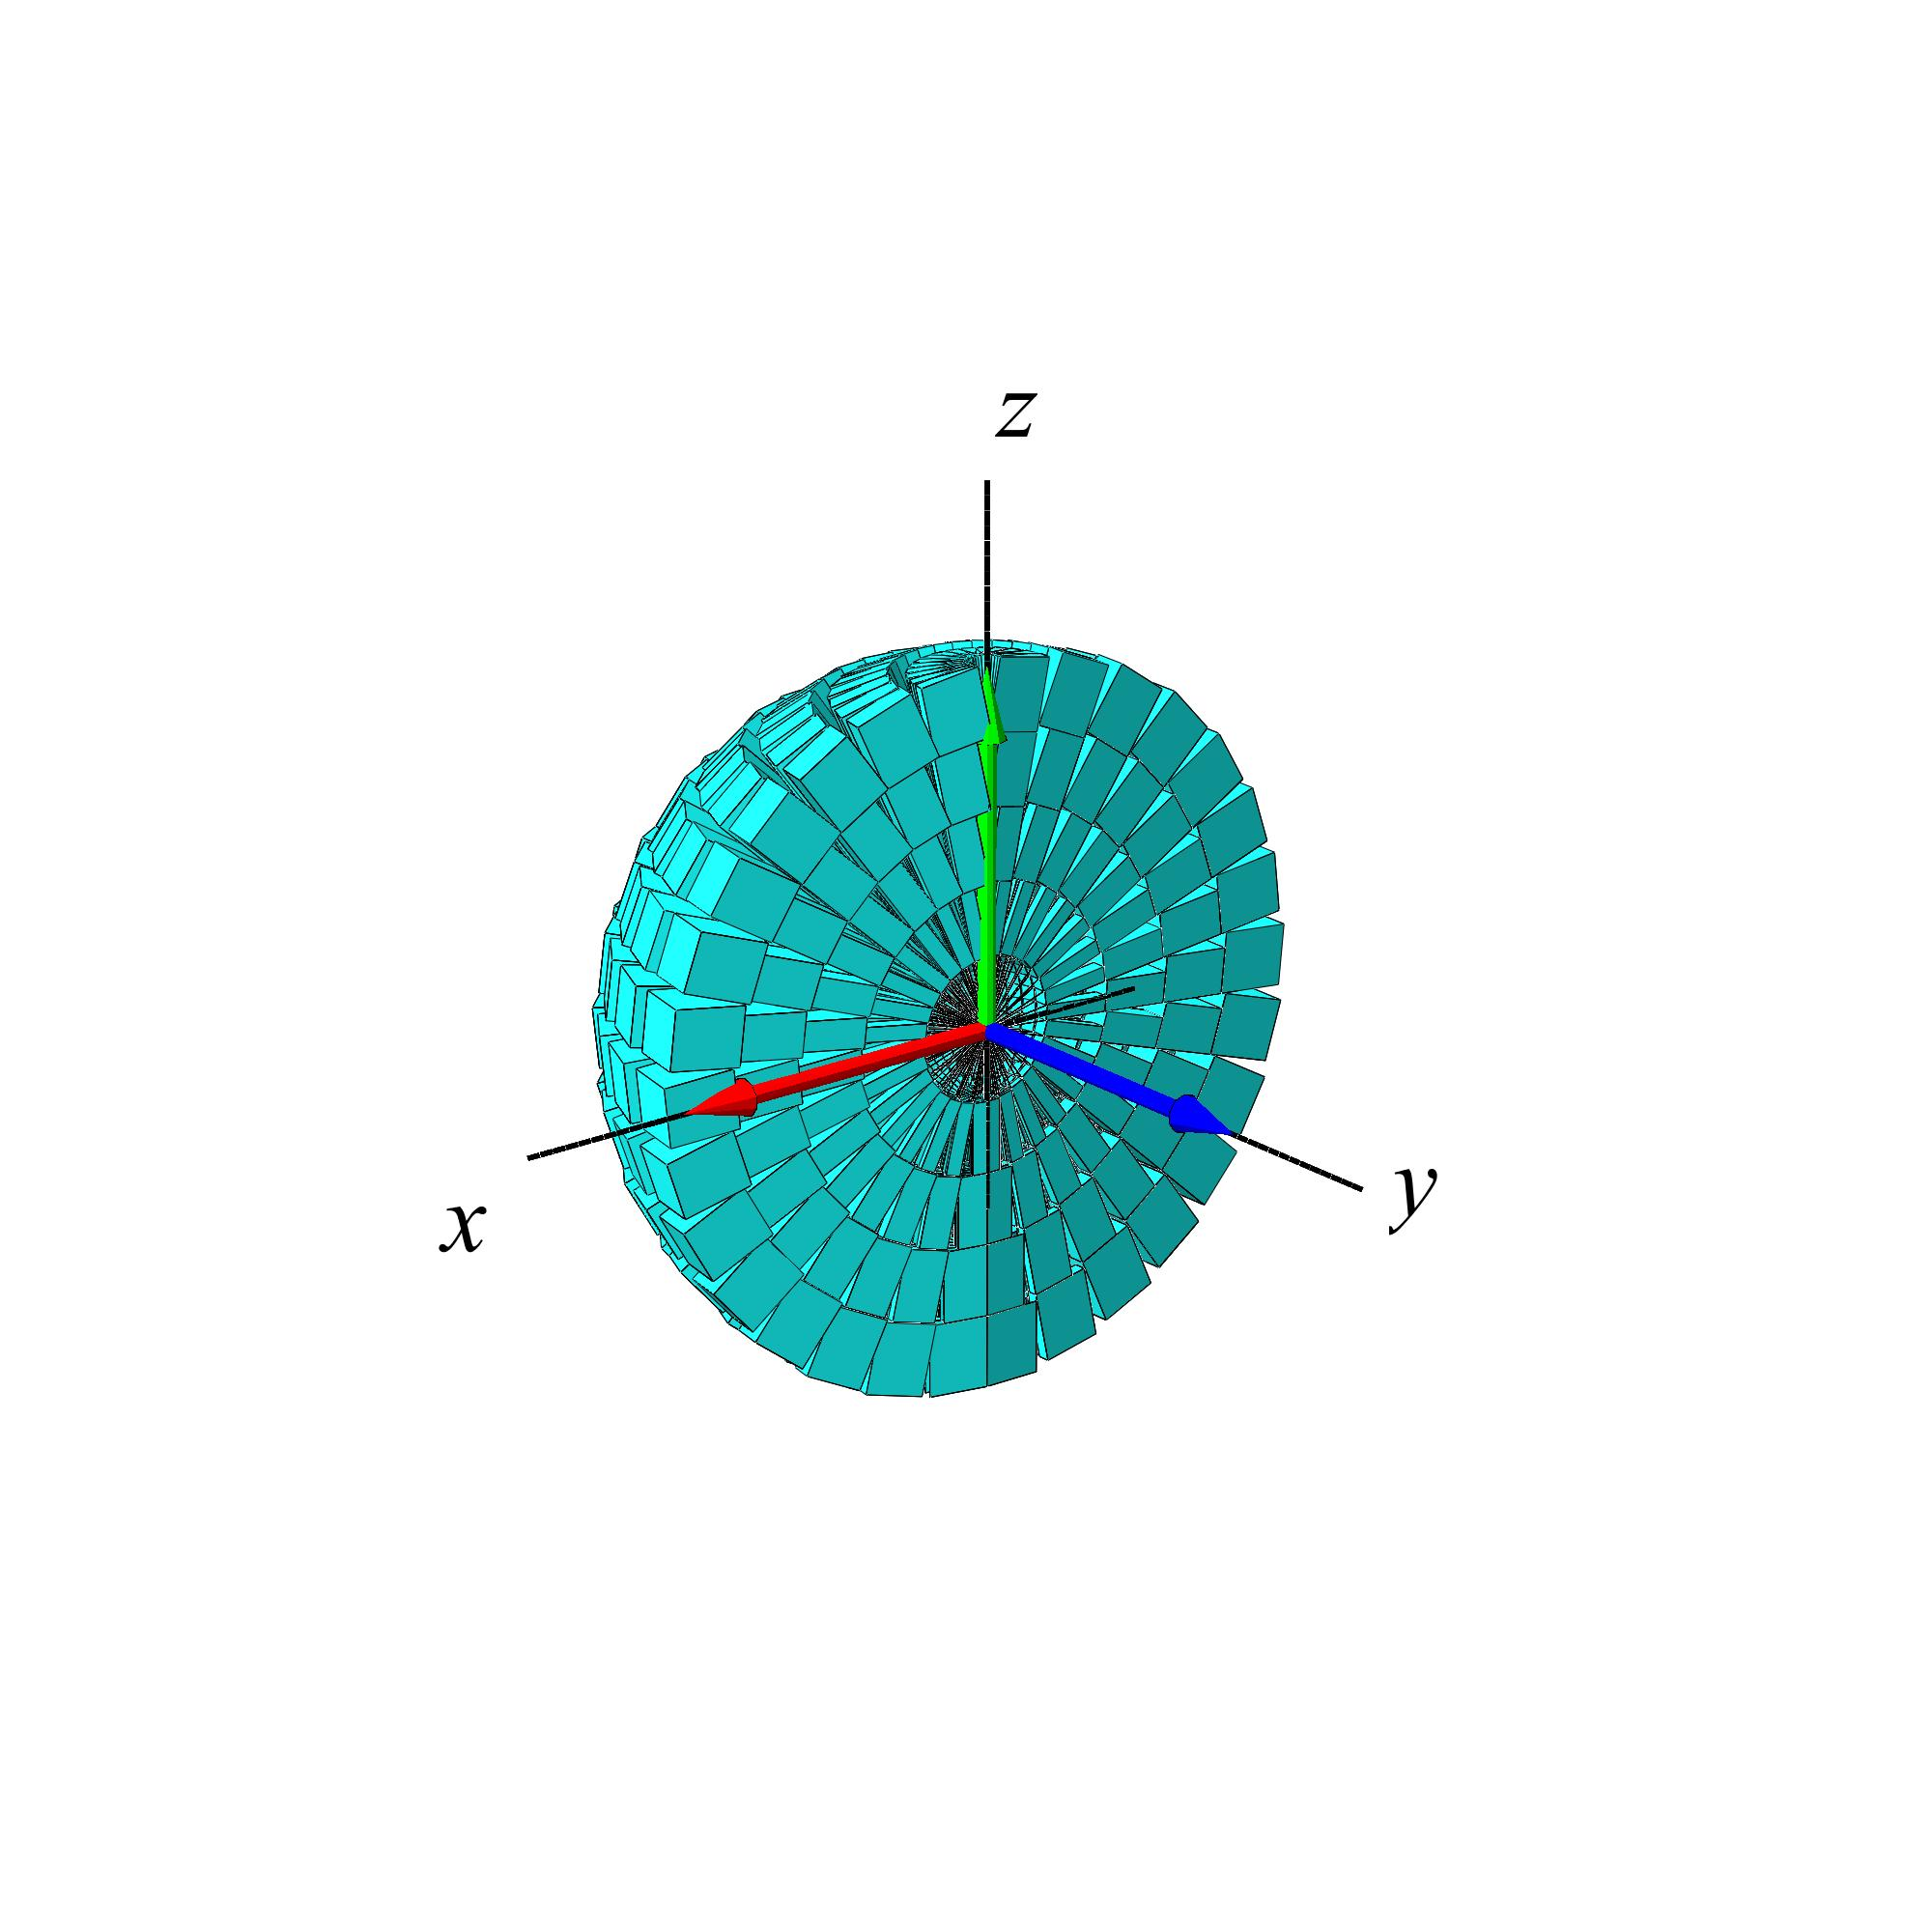
\includegraphics[height=75mm]{FIGS/plotSphereFillA3} \quad 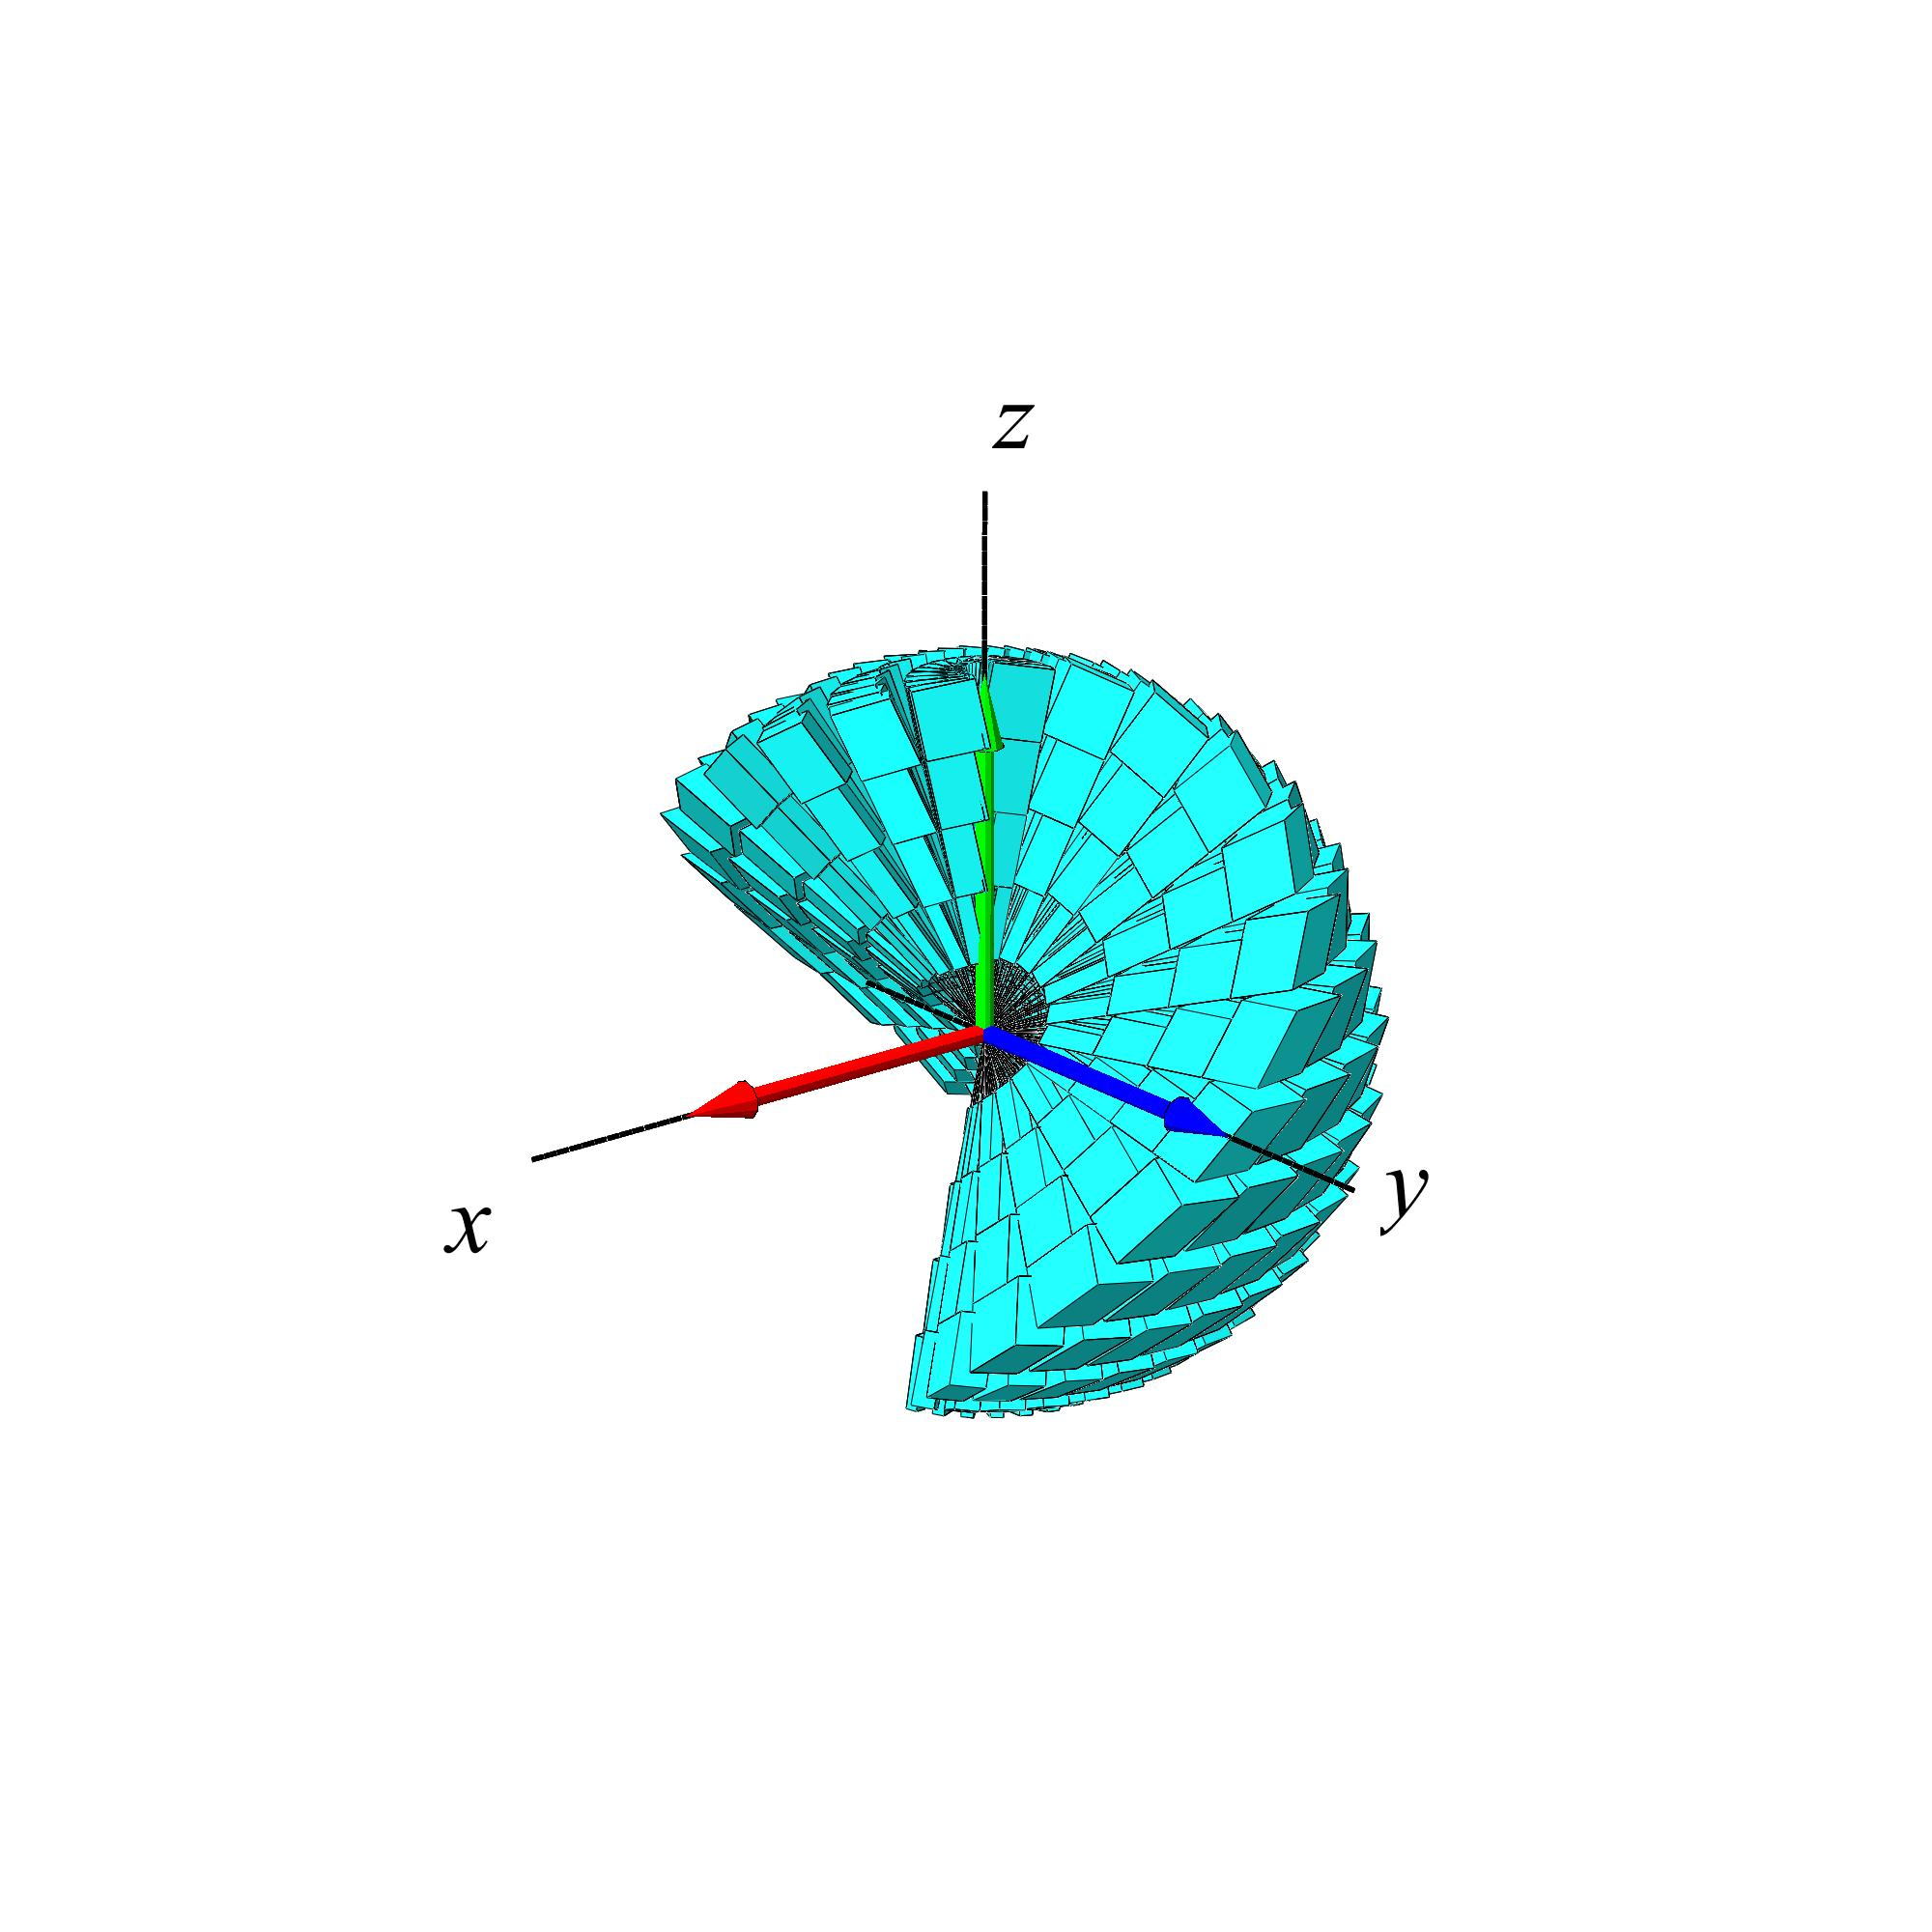
\includegraphics[height=75mm]{FIGS/plotSphereFillB3}}
\begin{center}
\caption{\small{To forskellige delvise kugle-fyldninger med parallelepipeda. Se Opgave \ref{exKuglefyld}.
}} \label{figSphereFillB}
\end{center}
\end{figure}



\begin{exercise} \label{exKuglefyld}
Kugle-parameterfremstillingerne i figur \ref{figSphereFillB} er henholdsvis følgende:
\begin{equation*}\begin{aligned}
{\bf r}_{1}(u, v, w) \, &= \, [\, w\sin(u)\cos(v), w\sin(u)\sin(v), w\cos(u)\,]  \\
{\bf r}_{2}(u, v, w) \, &= \, [\,w\sin(v)\cos(u+v), w\sin(v)\sin(u+v), w\cos(v) \,] \,\, ,
\end{aligned}
\end{equation*}
hvor parameterintervallerne i begge tilfælde er givet ved:
$$
\,\, u \in
[-\pi, 0]\,\, , \, \, v \in
[0, \pi]\,\, , \, \, w \in [0, 1] \quad .
$$
Bestem Jacobi-funktionerne for hver af de to parameterfremstillinger,
og vis, at begge de viste rumlige områder har volumenet $2\pi/3$, altså præcis halvdelen af
hele enheds-kuglens volumen.
\end{exercise}







%%%%%%%%%%%%%%%%%%%%%%%%%%%%%%%%%%%%%%%%%%%%%%%%%%%
%%%%%%%%%%%%%%%%%%%%%%%%%%%%%%%%%%%%%%%%%%%%%%%%%%%

\subsubsection{Masse} \label{subsubsecRumMass}
Hvis vi nu antager, at
hvert enkelt parallelepipedum givet ved
(\ref{eqApp3}) tildeles en konstant massetæthed
som er givet ved værdien af funktionen $f(x,y,z)$
på stedet  ${\bf r}(u_{i}, v_{j}, w_{k})$, så
bliver massen af det $(i, j, k)$'te
parallelepipedum:

\begin{equation}
\label{eqDeltaM3}
\begin{aligned}
\Delta \M_{ijk} \, = \, &f(x(u_{i}, v_{j}, w_{k}), y(u_{i}, v_{j},
w_{k}), z(u_{i}, v_{j}, w_{k})) \, \Jac_{\bf r}(u_{i}, v_{j}, w_{k})
\cdot\delta_{u} \delta_{v} \delta_{w} \,
\\ = \, &f( {\bf r}(u_{i}, v_{j}, w_{k})) \, \Jac_{\bf r}(u_{i},
v_{j}, w_{k}) \cdot\delta_{u} \delta_{v} \delta_{w} \quad .
\end{aligned}
\end{equation}


Den totale masse af hele systemet af
appproksimerende parallelepipeda er derfor
følgende, som nødvendigvis er en god
approksimation til massen af hele det rumlige
område:
\begin{equation}
\begin{aligned}
 \M_{\app}(n,m,q) \, = \,
&\sum_{k=1}^{q}\sum_{j=1}^{m} \sum_{i=1}^{n} \Delta \M_{ijk} \,
\\ = \,
 &\sum_{k=1}^{q}\sum_{j=1}^{m}\sum_{i=1}^{n}f({\bf r}(u_{i}, v_{j}, w_{k}))\,\Jac_{\bf r}(u_{i}, v_{j}, w_{k}) \cdot \delta_{u} \delta_{v} \delta_{w}
\quad .
\end{aligned}
\end{equation}

Dette er en tredobbelt integralsum for den kontinuerte funktion
$f({\bf r}(u,v,w))\,\Jac_{\bf r}(u, v,w)$ over parameter-kassen
$\,[a, b]\times[c, d]\times[h, l]\,$. Vi får i grænsen, hvor $n$,
$m$ og $q$ går mod uendelig:
\begin{equation}
\begin{aligned}
&\M_{\app}(n,m,q)\, \to \, \M \, = \,
\int_{h}^{l}\int_{c}^{d}\int_{a}^{b}f({\bf r}(u,v,w))\Jac_{\bf
r}(u, v, w)\,du \,dv\, dw \\ &\text{for} \quad n, m, q \to
\infty \quad.
\end{aligned}
\end{equation}

Dermed har vi motiveret definitionen af massen af et
parametriseret område med massetætheden $f({\bf r}(u, v, w))$ og
dermed også den generelle definition
\ref{defRumInt} af rumintegralet.


\begin{exercise}
I figur \ref{figKugle13} betragtes følgende parametrisering af et
rumligt område:
\begin{equation}
{\bf r}(u, v, w) \, = \, (u\,\sin(v)\cos(w), u\,\sin(v)\sin(w),
u\,\cos(v) ) \quad ,
\end{equation}
hvor $u \in [1/2, 1 ]$, $v \in [\pi/3,
2\pi/3]$, og $w \in [-\pi, \pi]$.
Ved afbildning af det kasseformede parameterområde forventes ialt
$6$ sideflader for billed-mæng\-den, dvs. for det rumlige område, der fremkommer ved parameterfremstillingen. Vi ser på figuren kun tre af de
$6$ sideflader. Hvor er de andre og hvordan ser de ud?
\end{exercise}





\begin{figure}[h]
\centerline{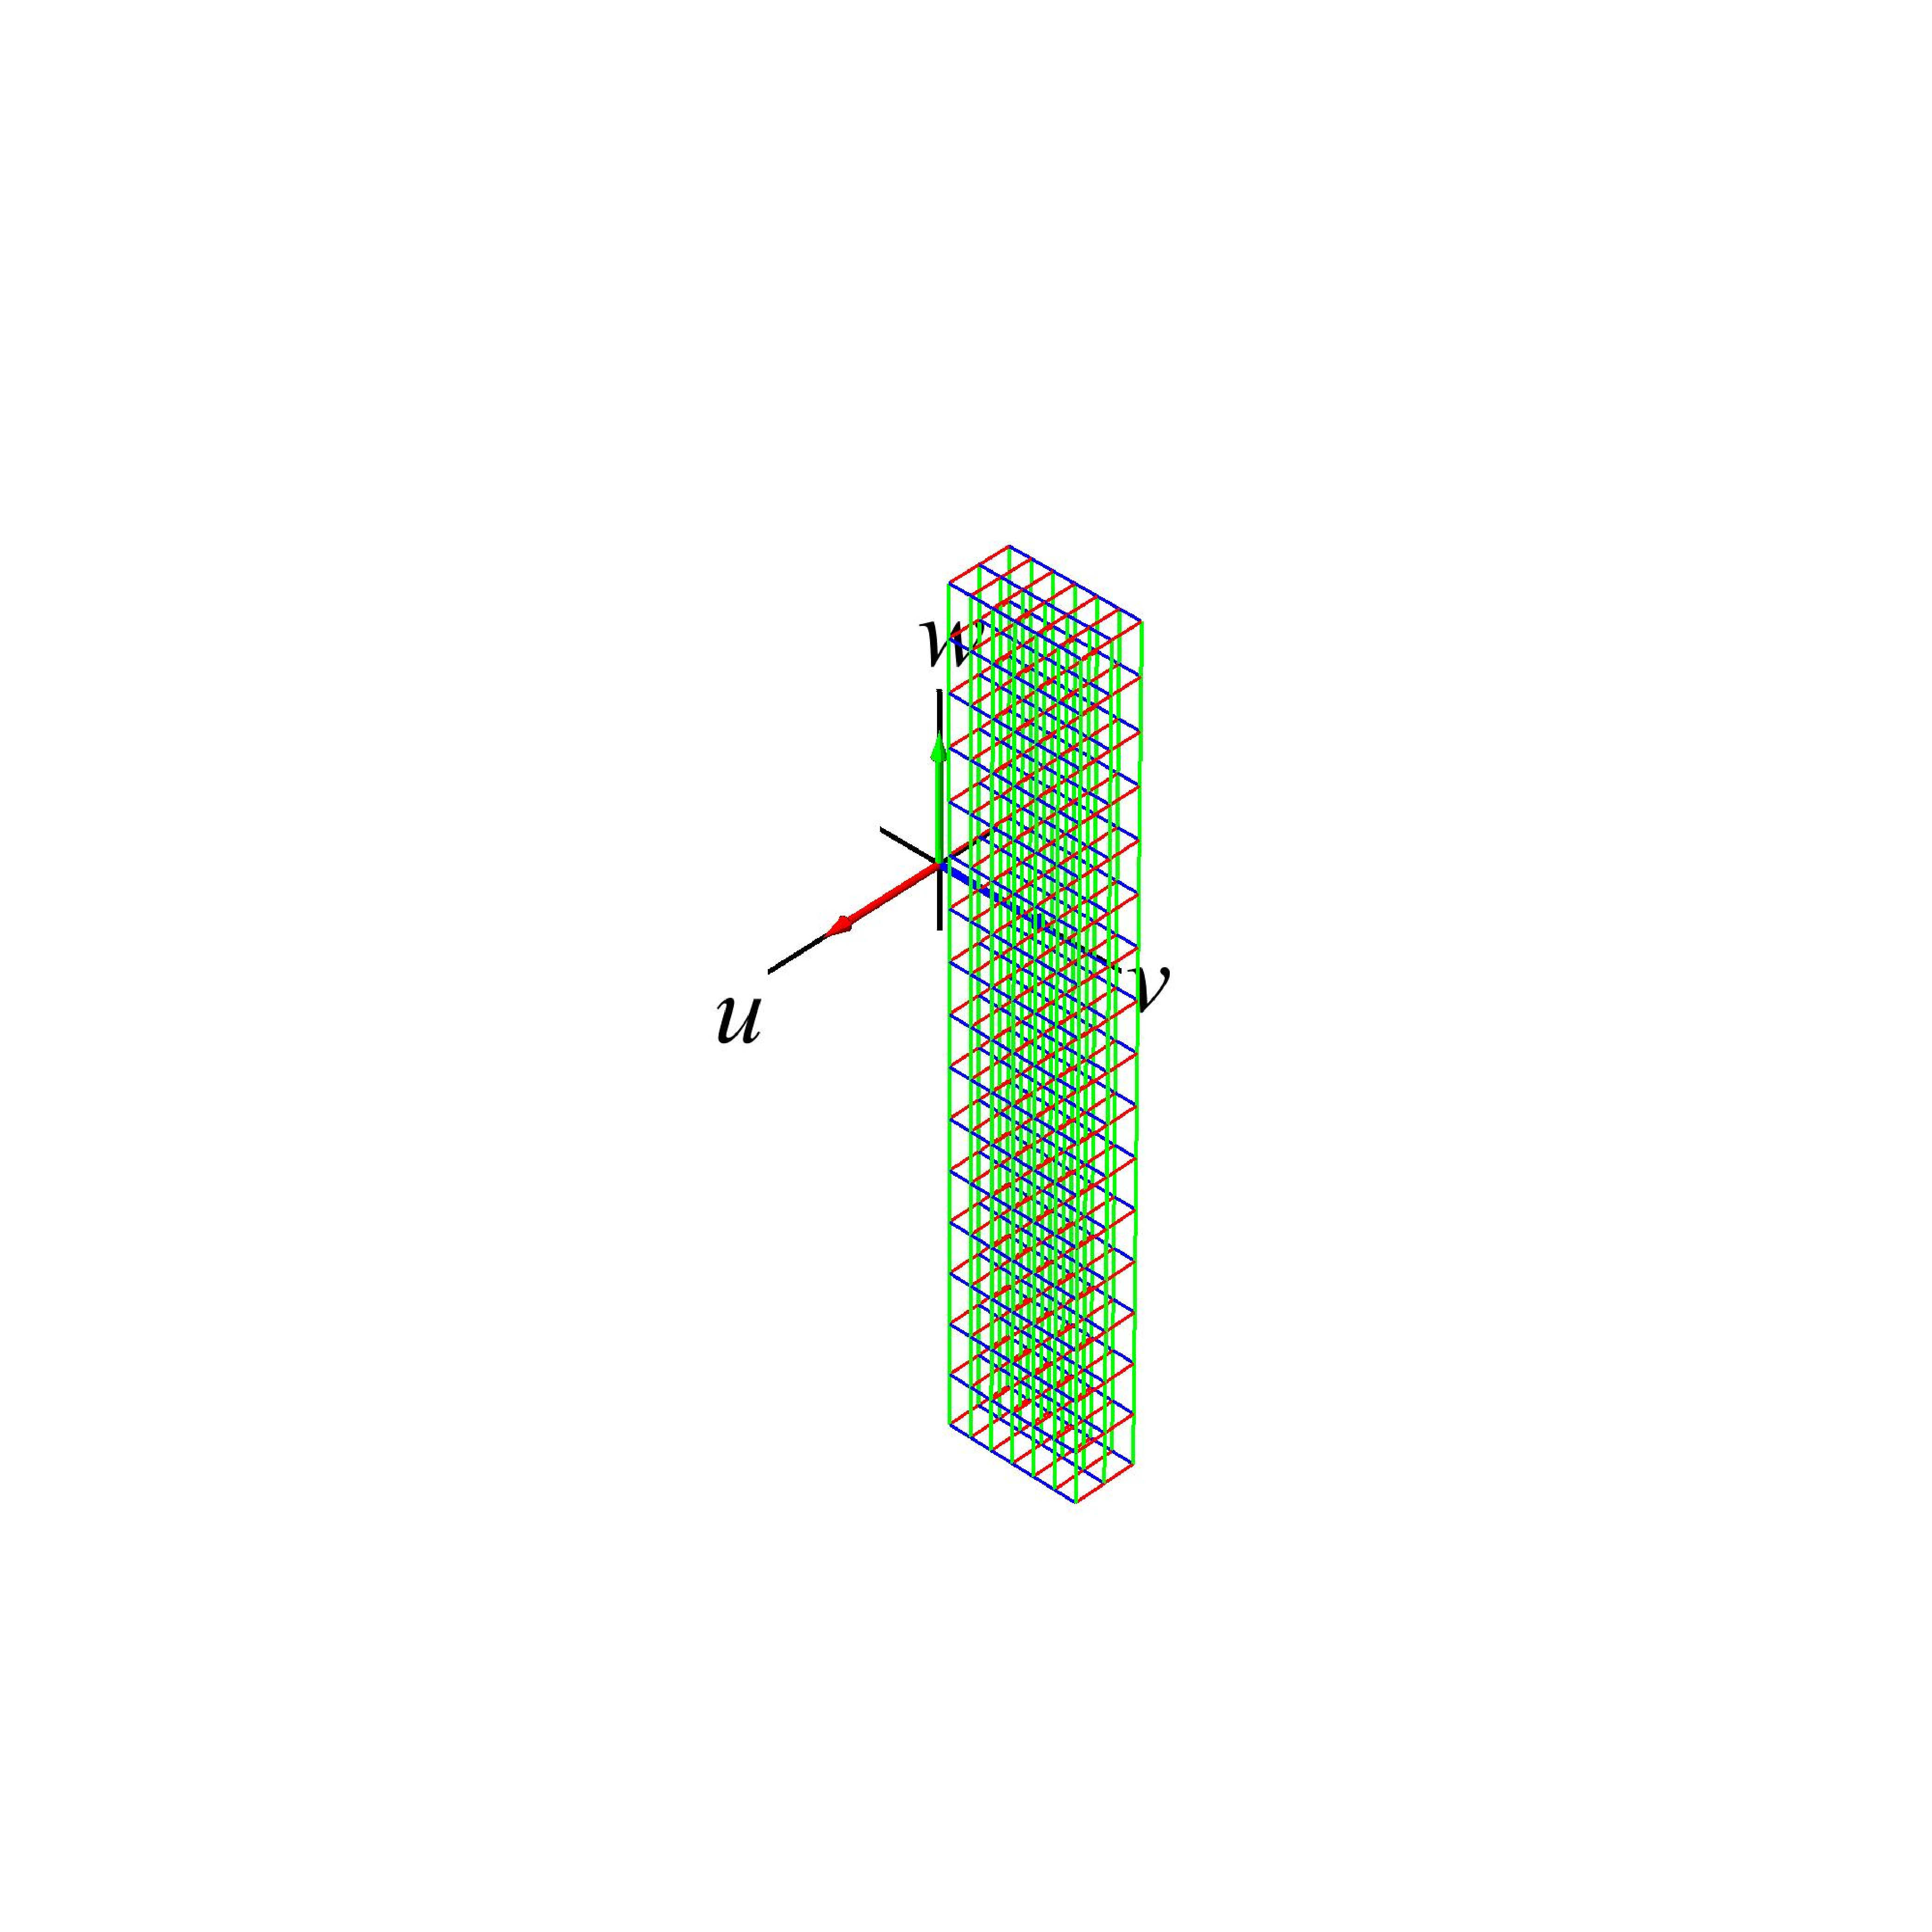
\includegraphics[height=50mm]{FIGS/plotSpherePart1} 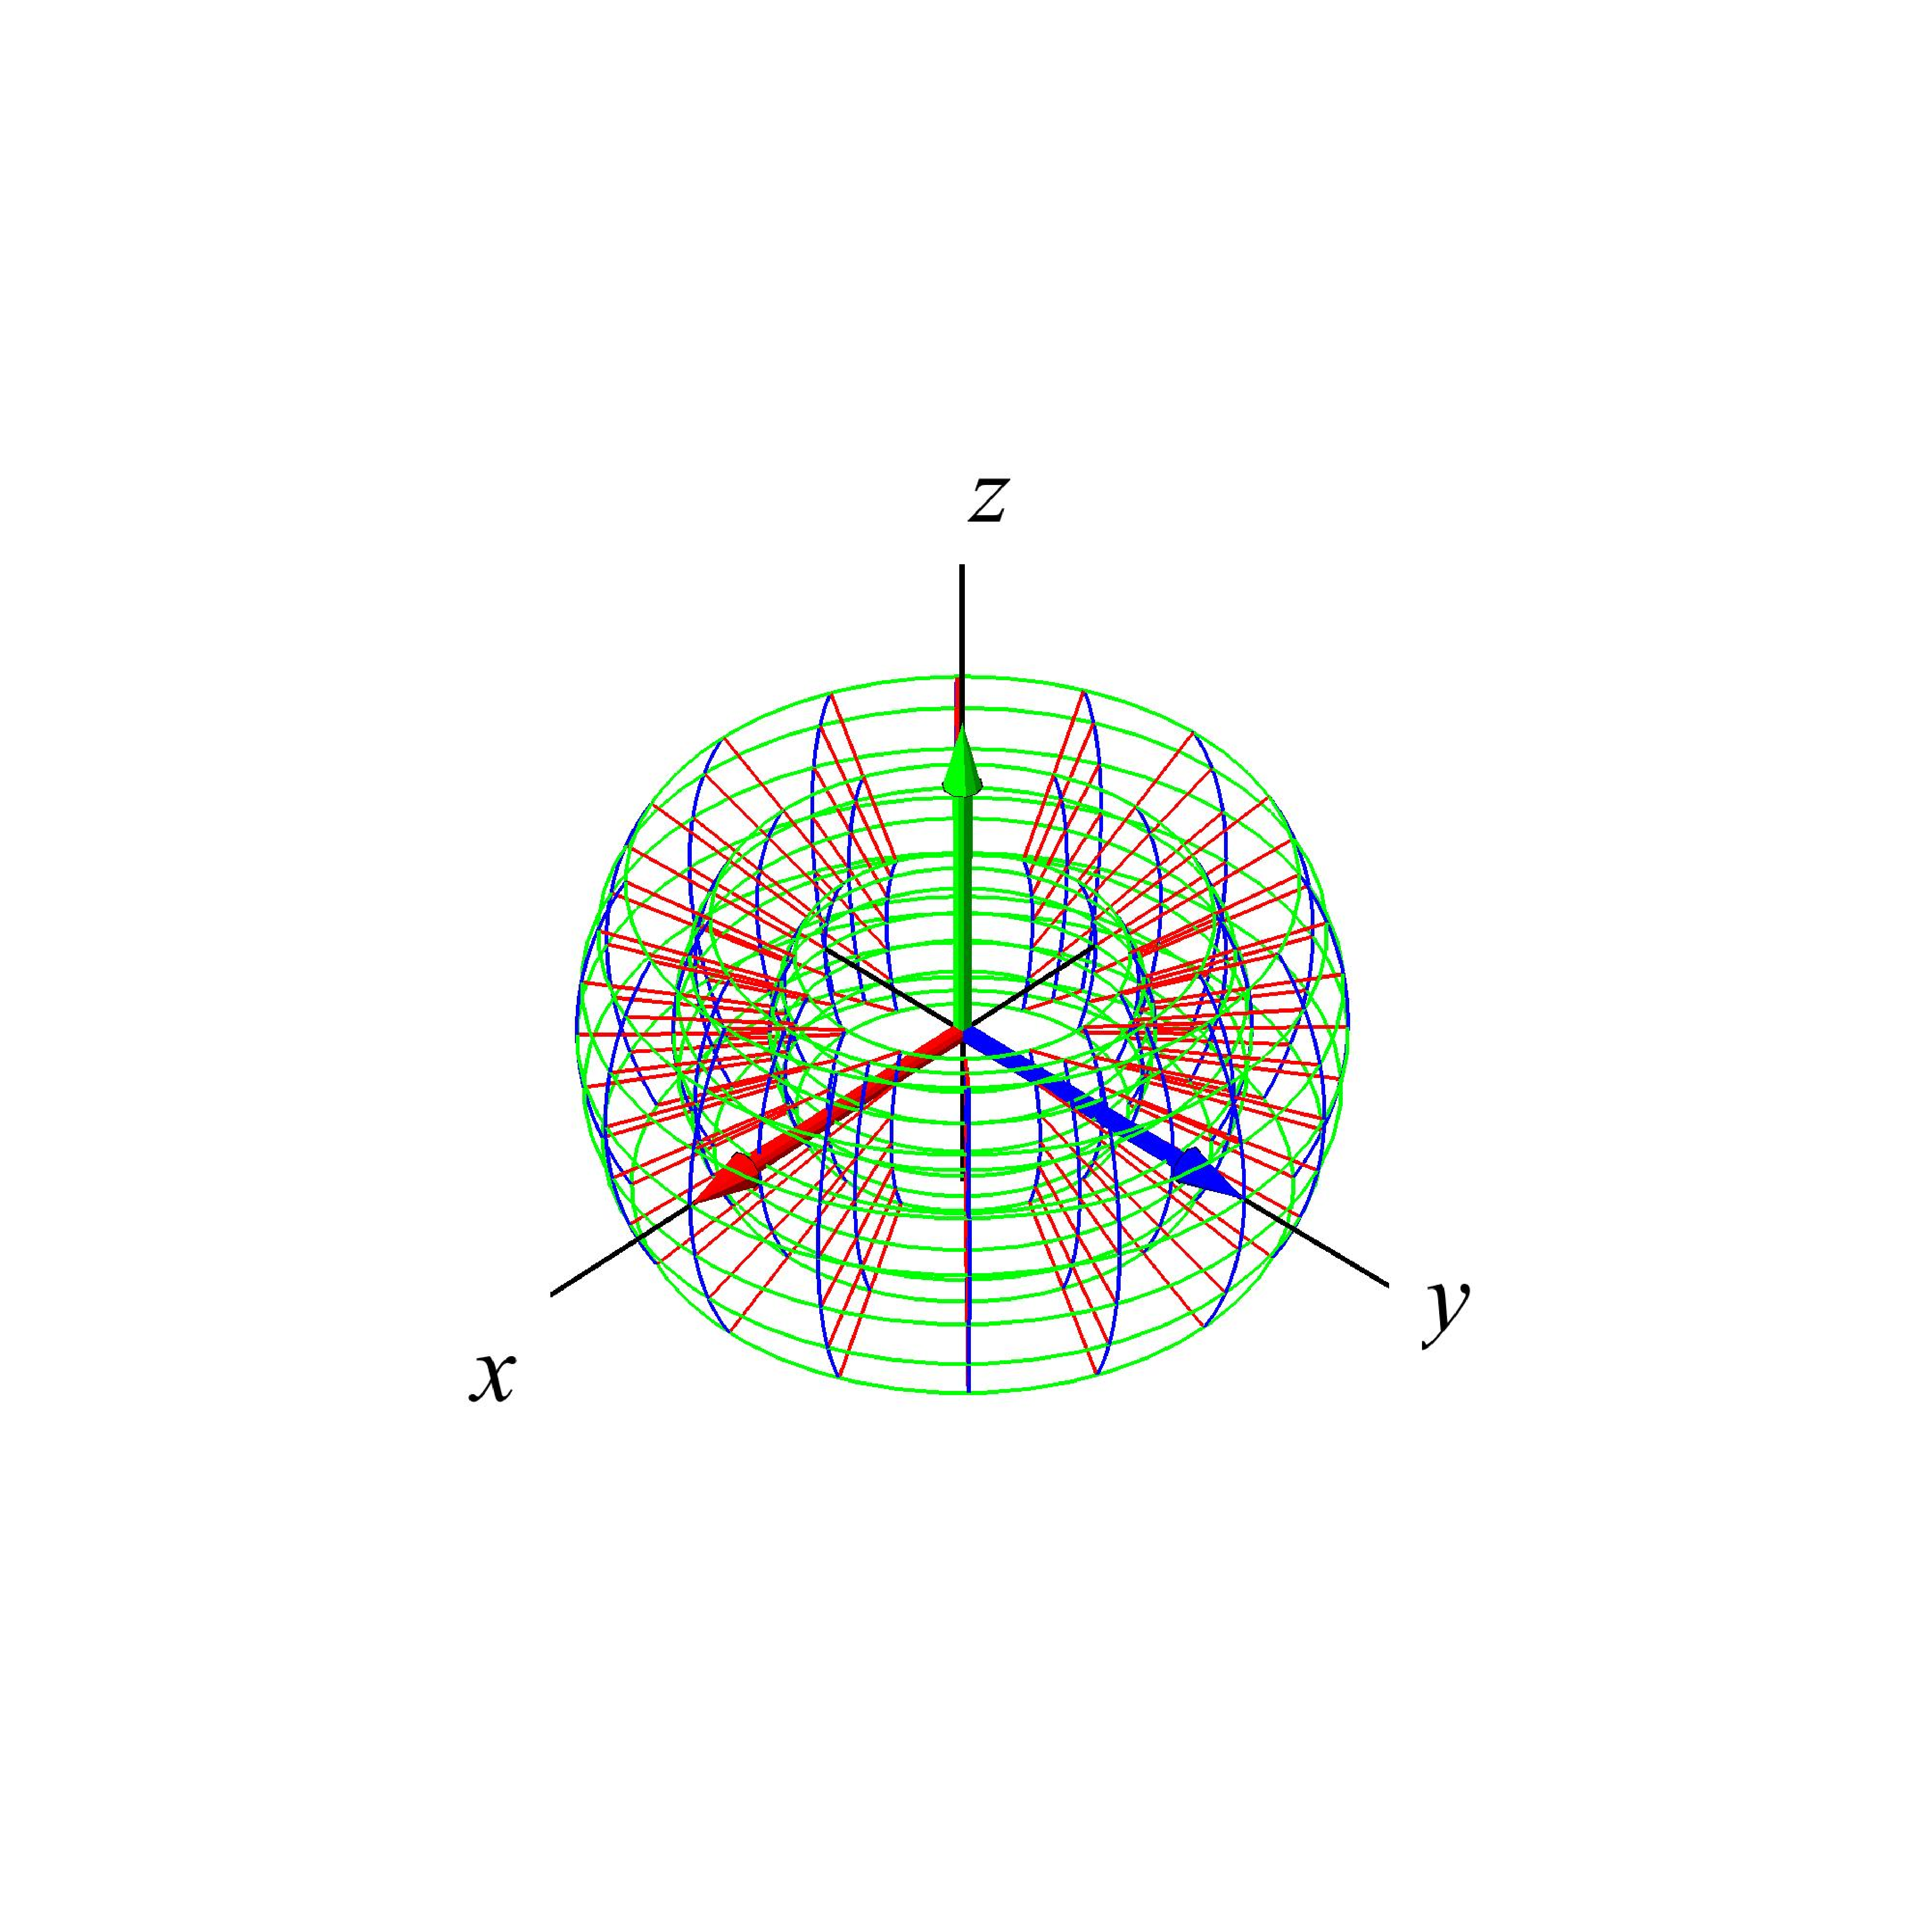
\includegraphics[height=50mm]{FIGS/plotSpherePart3}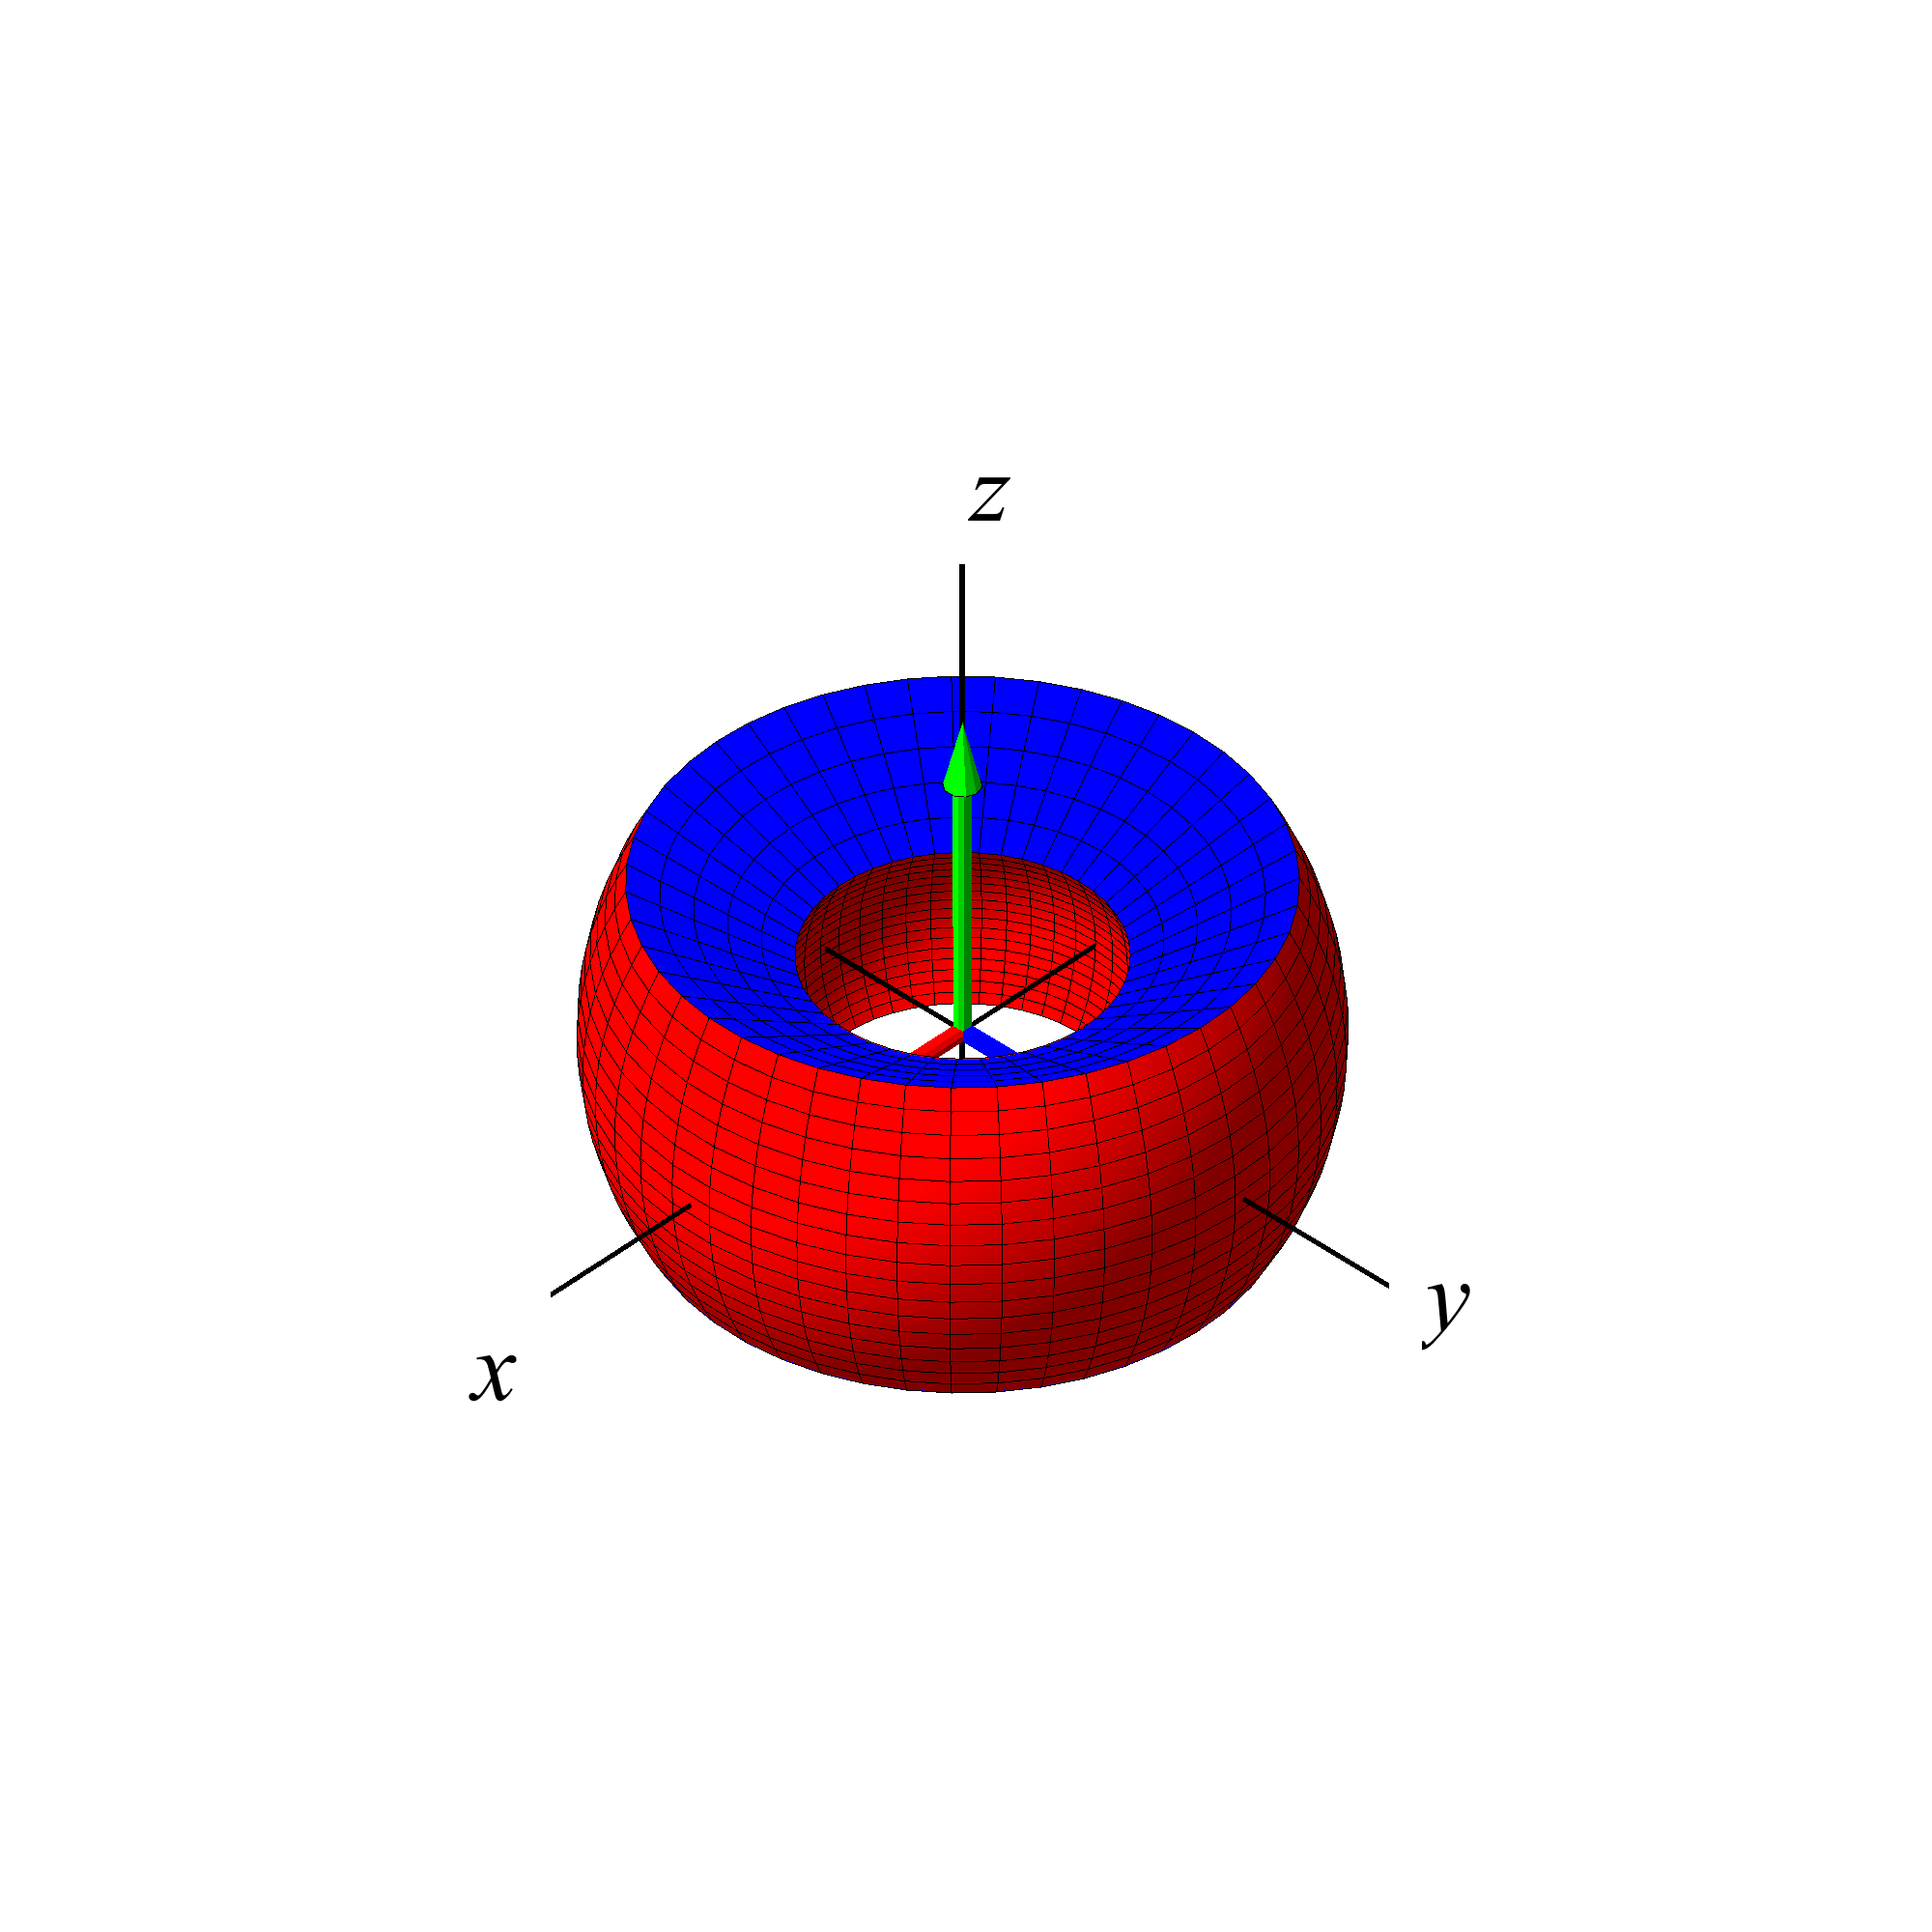
\includegraphics[height=50mm]{FIGS/plotSpherePart2}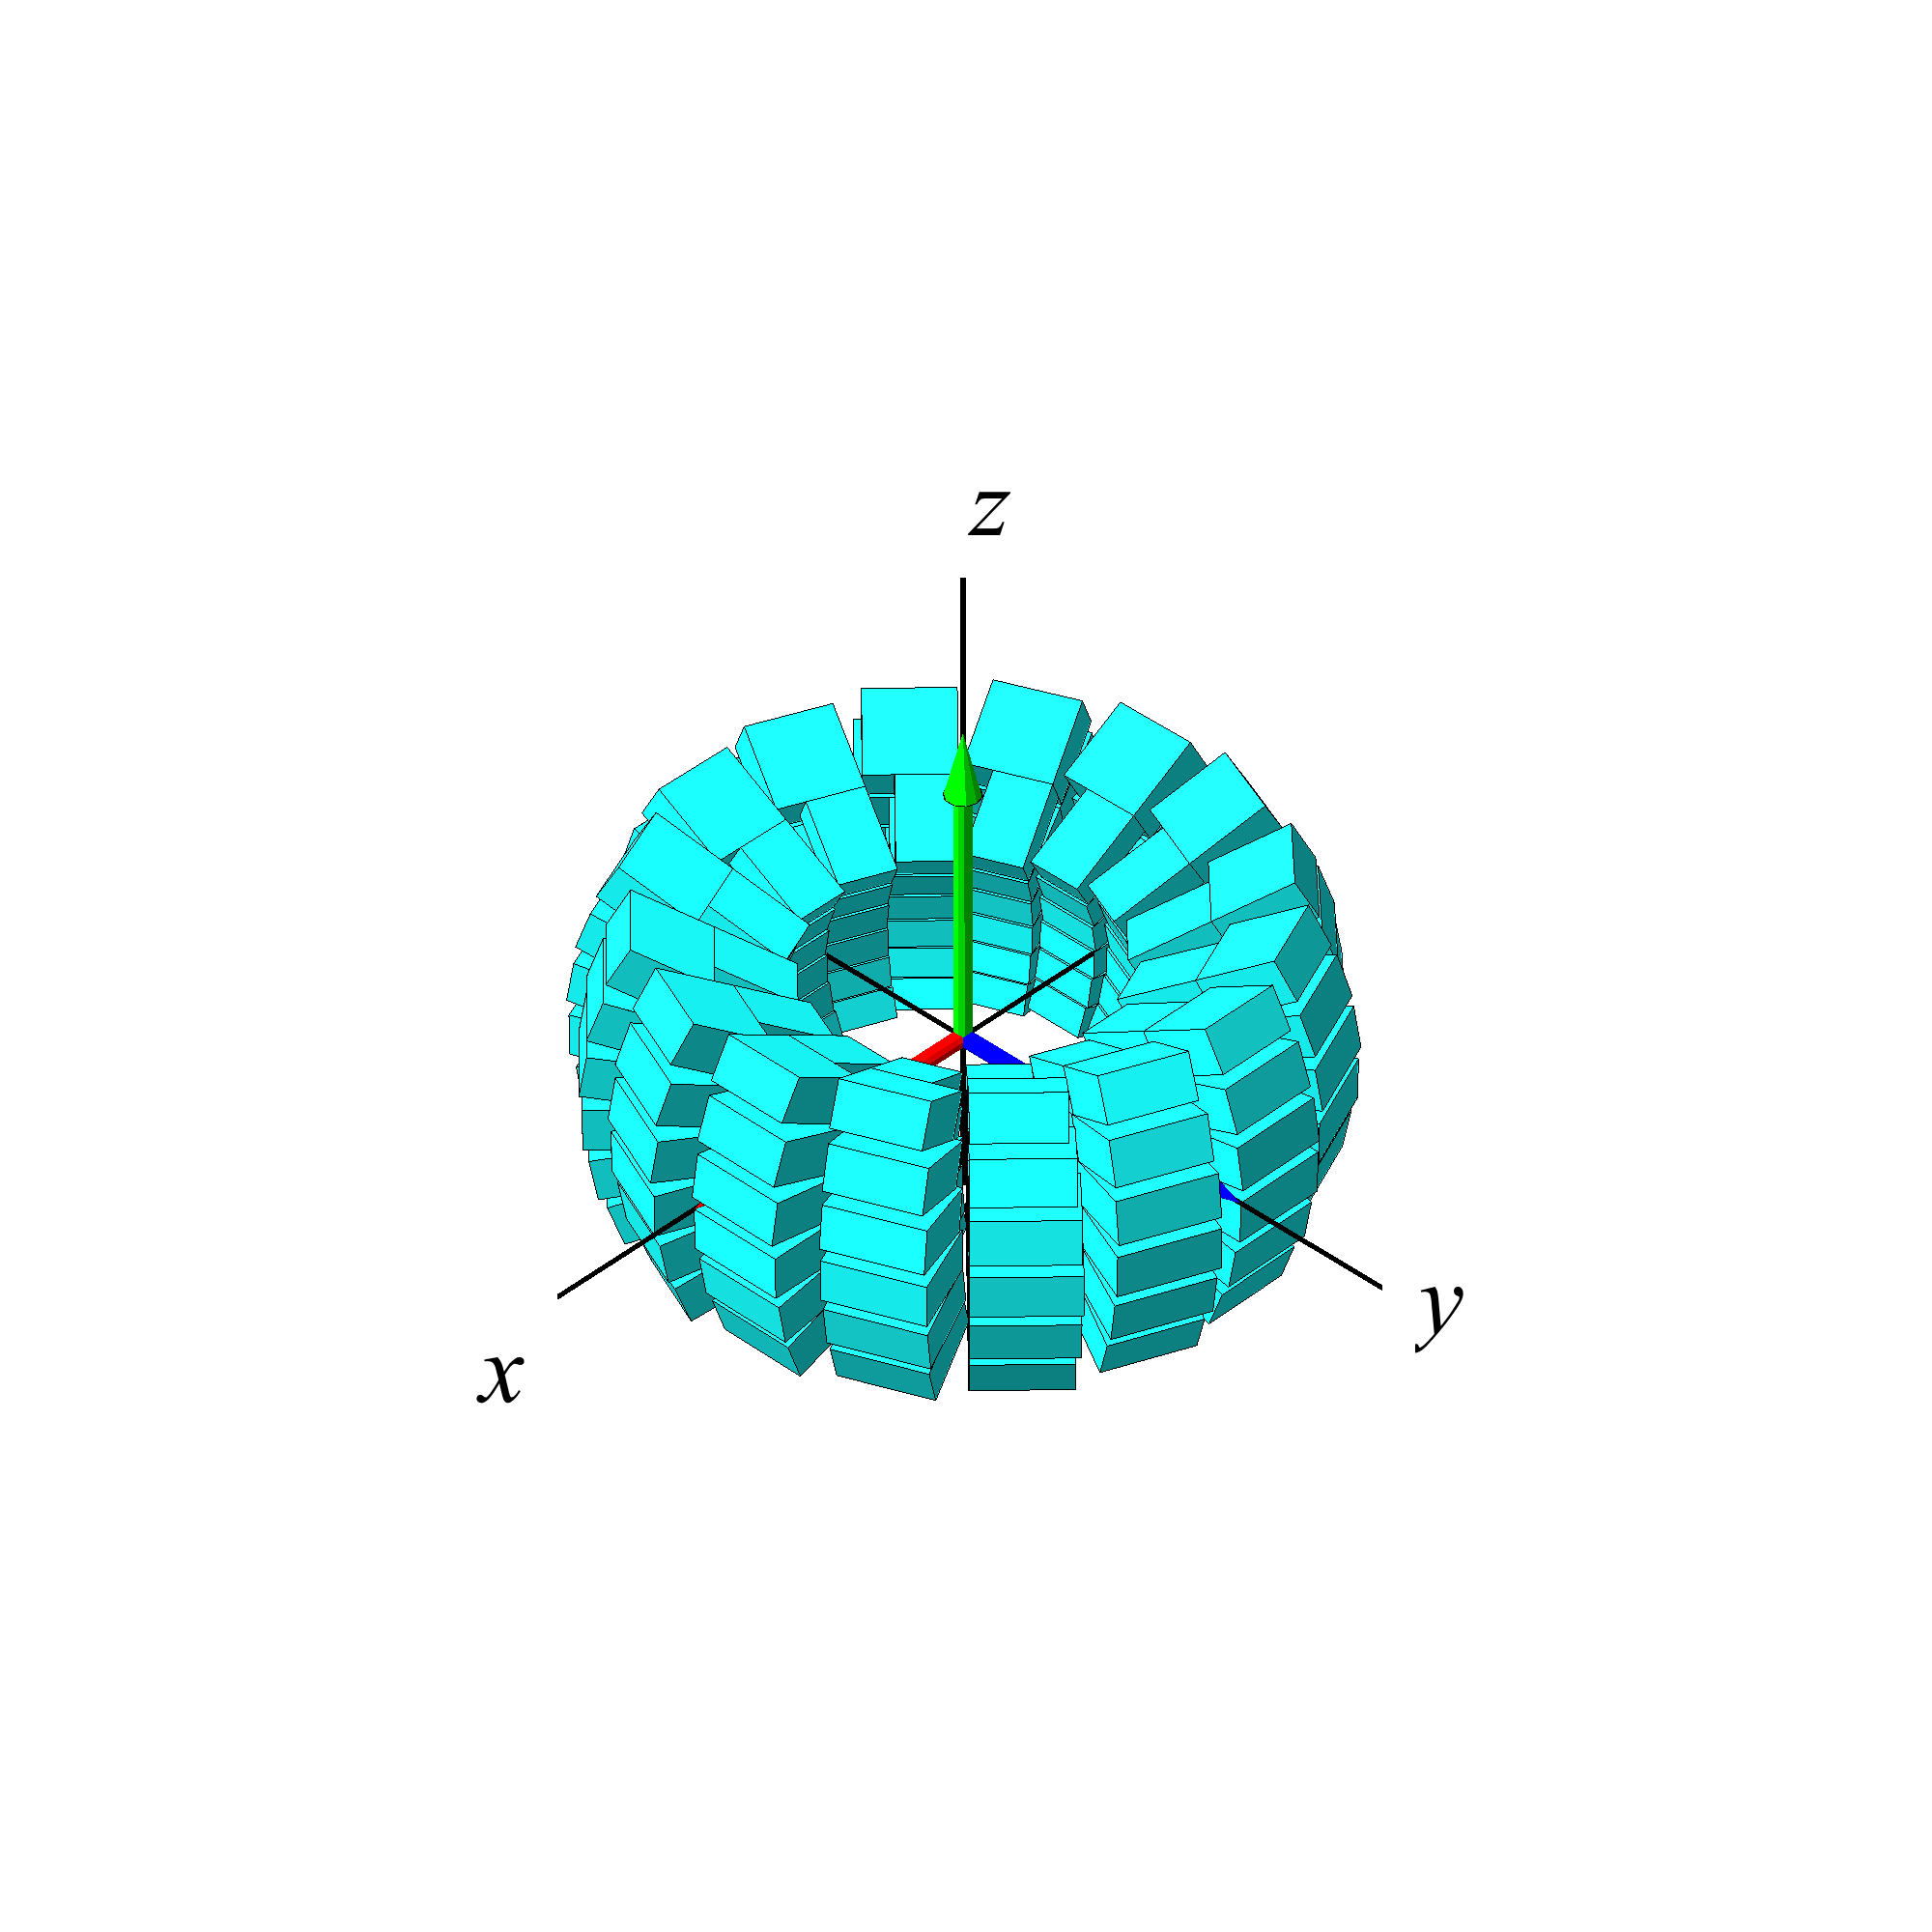
\includegraphics[height=50mm]{FIGS/plotSpherePart4} }
\begin{center}
\caption{\small{Dette {\em rumlige} område er
givet ved parameterfremstillingen ${\bf r}(u, v,
w) \, = \, (u\,\sin(v)\cos(w), u\,\sin(v)\sin(w),
u\,\cos(v) ) \,\,, \,\, u \in [1/2, 1 ]\,\, , \, \,
v \in [\pi/3, 2\pi/3]\,\, , \, \, w \in [-\pi, \pi] $.
Parameterkassen, koordinatkurverne, billedet af det rumlige område ved parameterfremstillingen og et system af
volumen-approksimerende parallellepipida er vist.}} \label{figKugle13}
\end{center}
\end{figure}

\begin{figure}[h]
\centerline{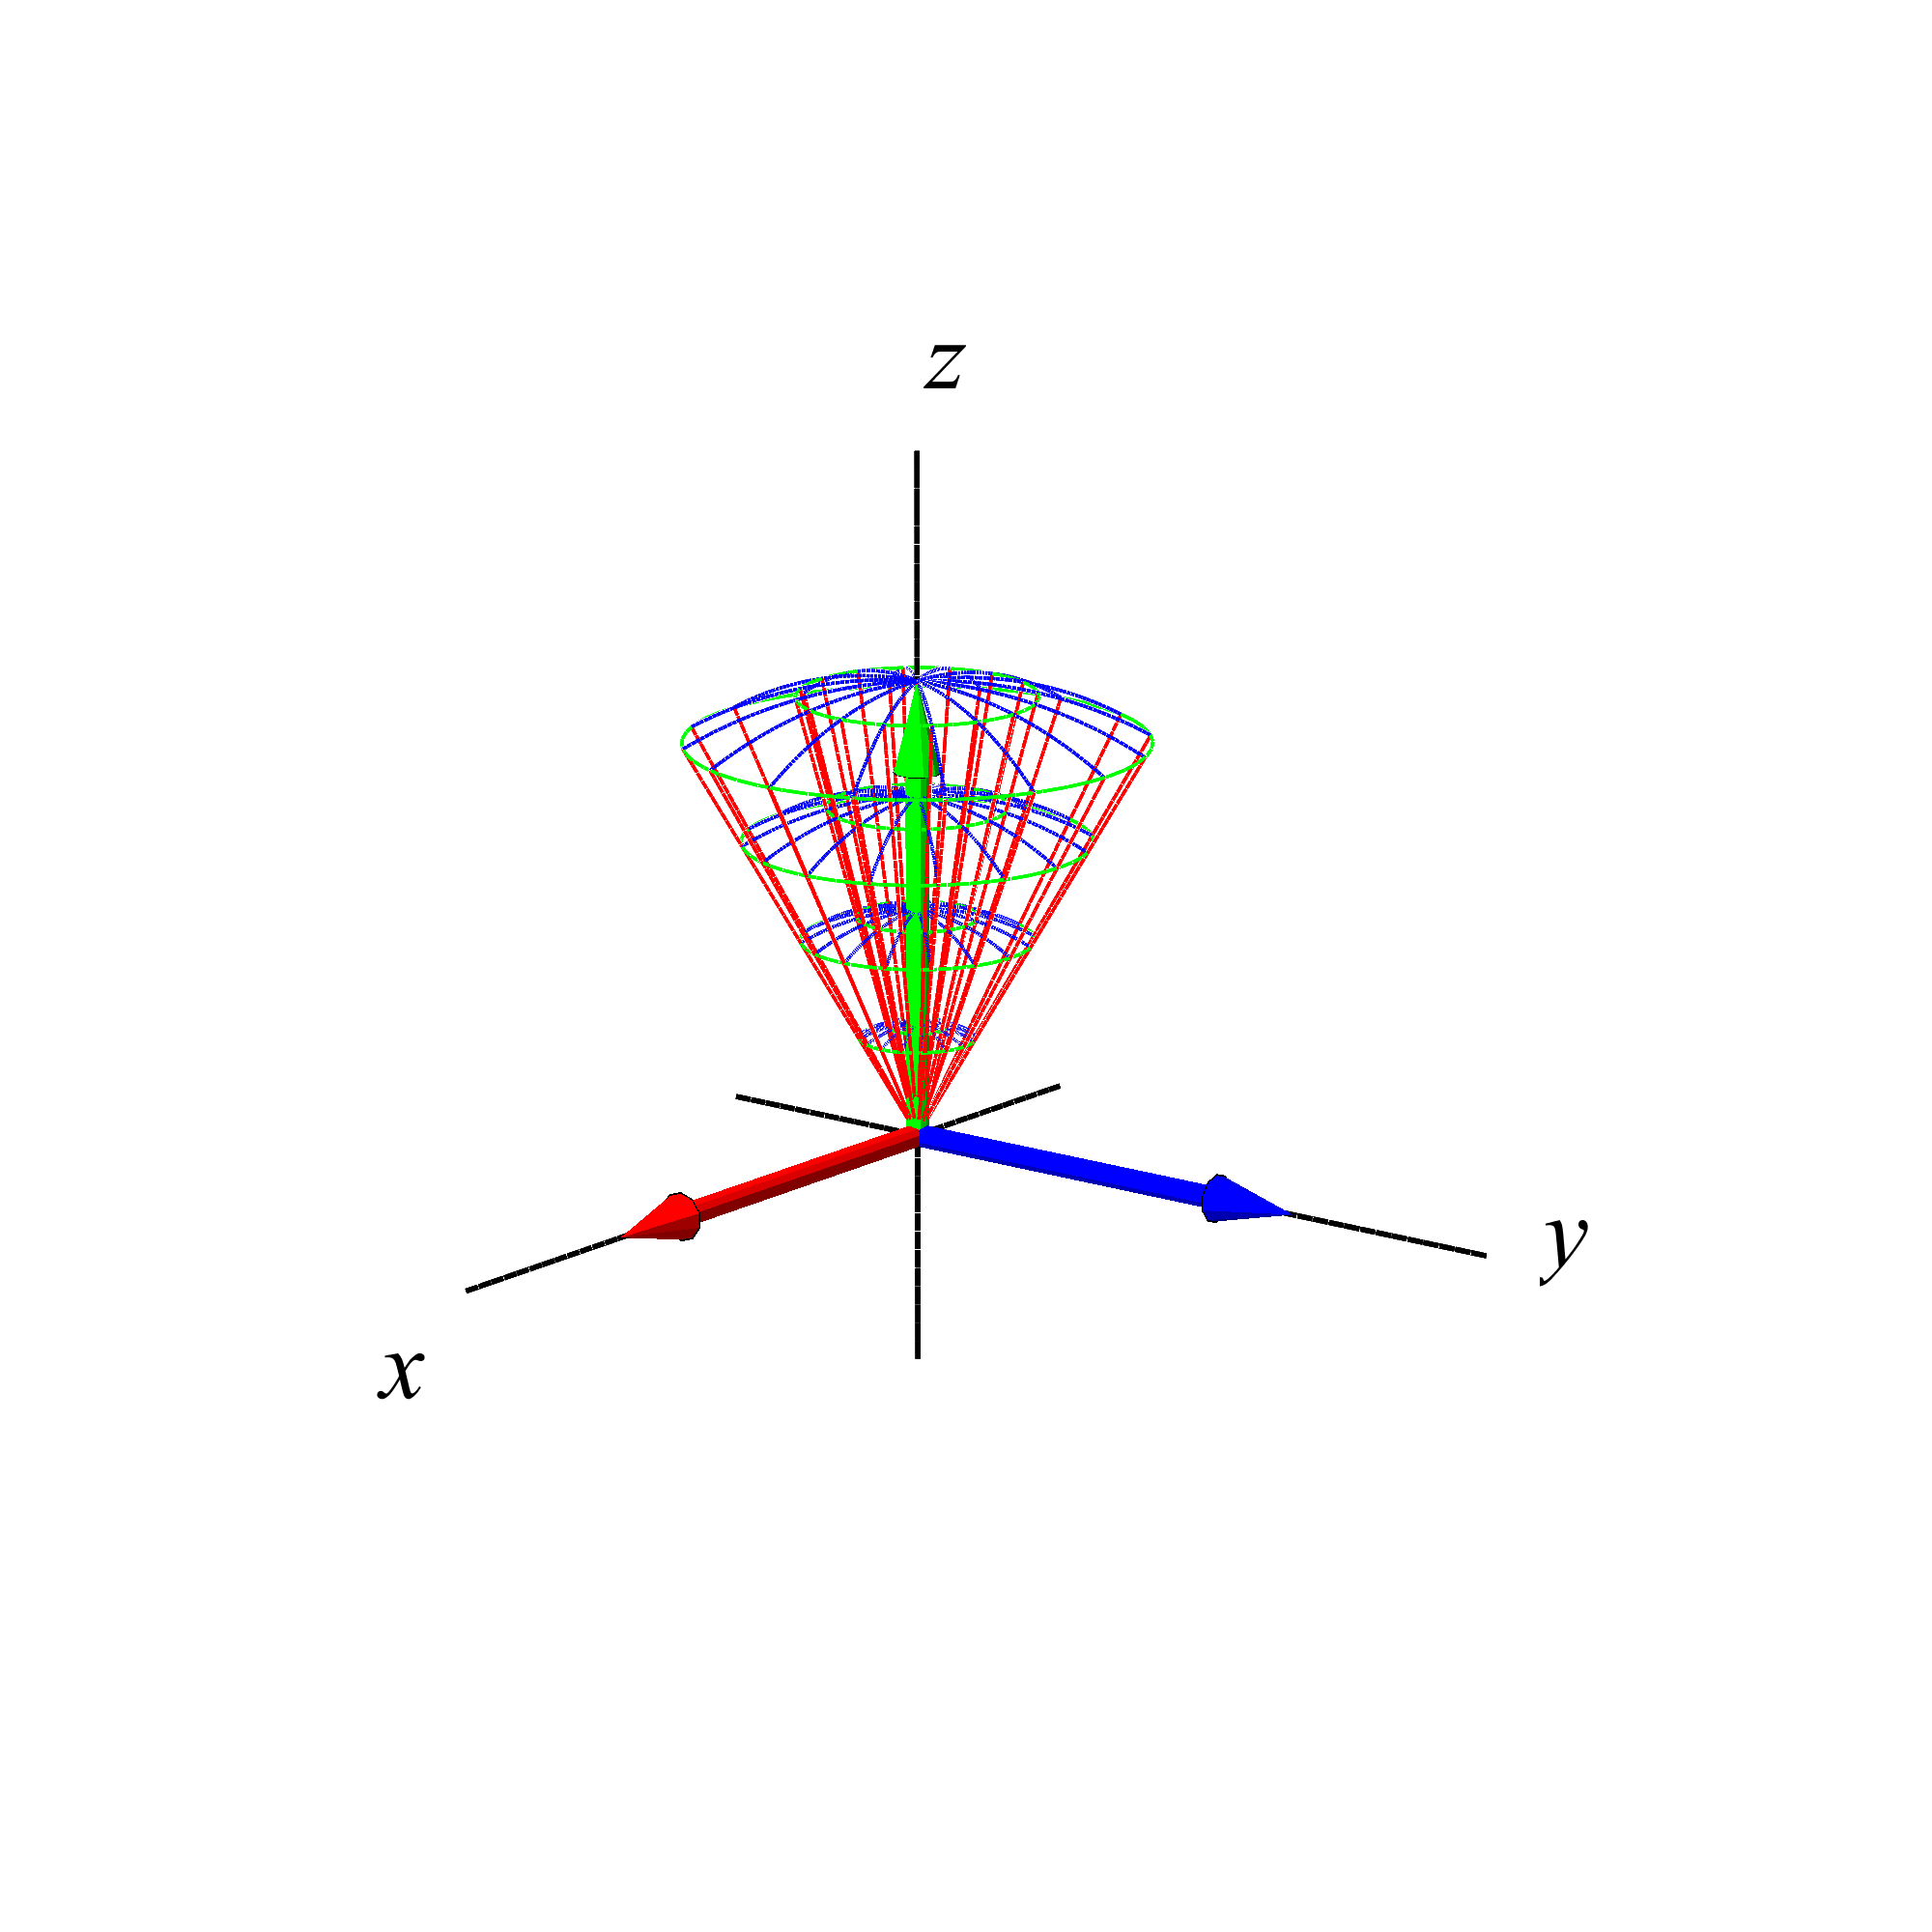
\includegraphics[height=50mm]{FIGS/plotSphereProp2} 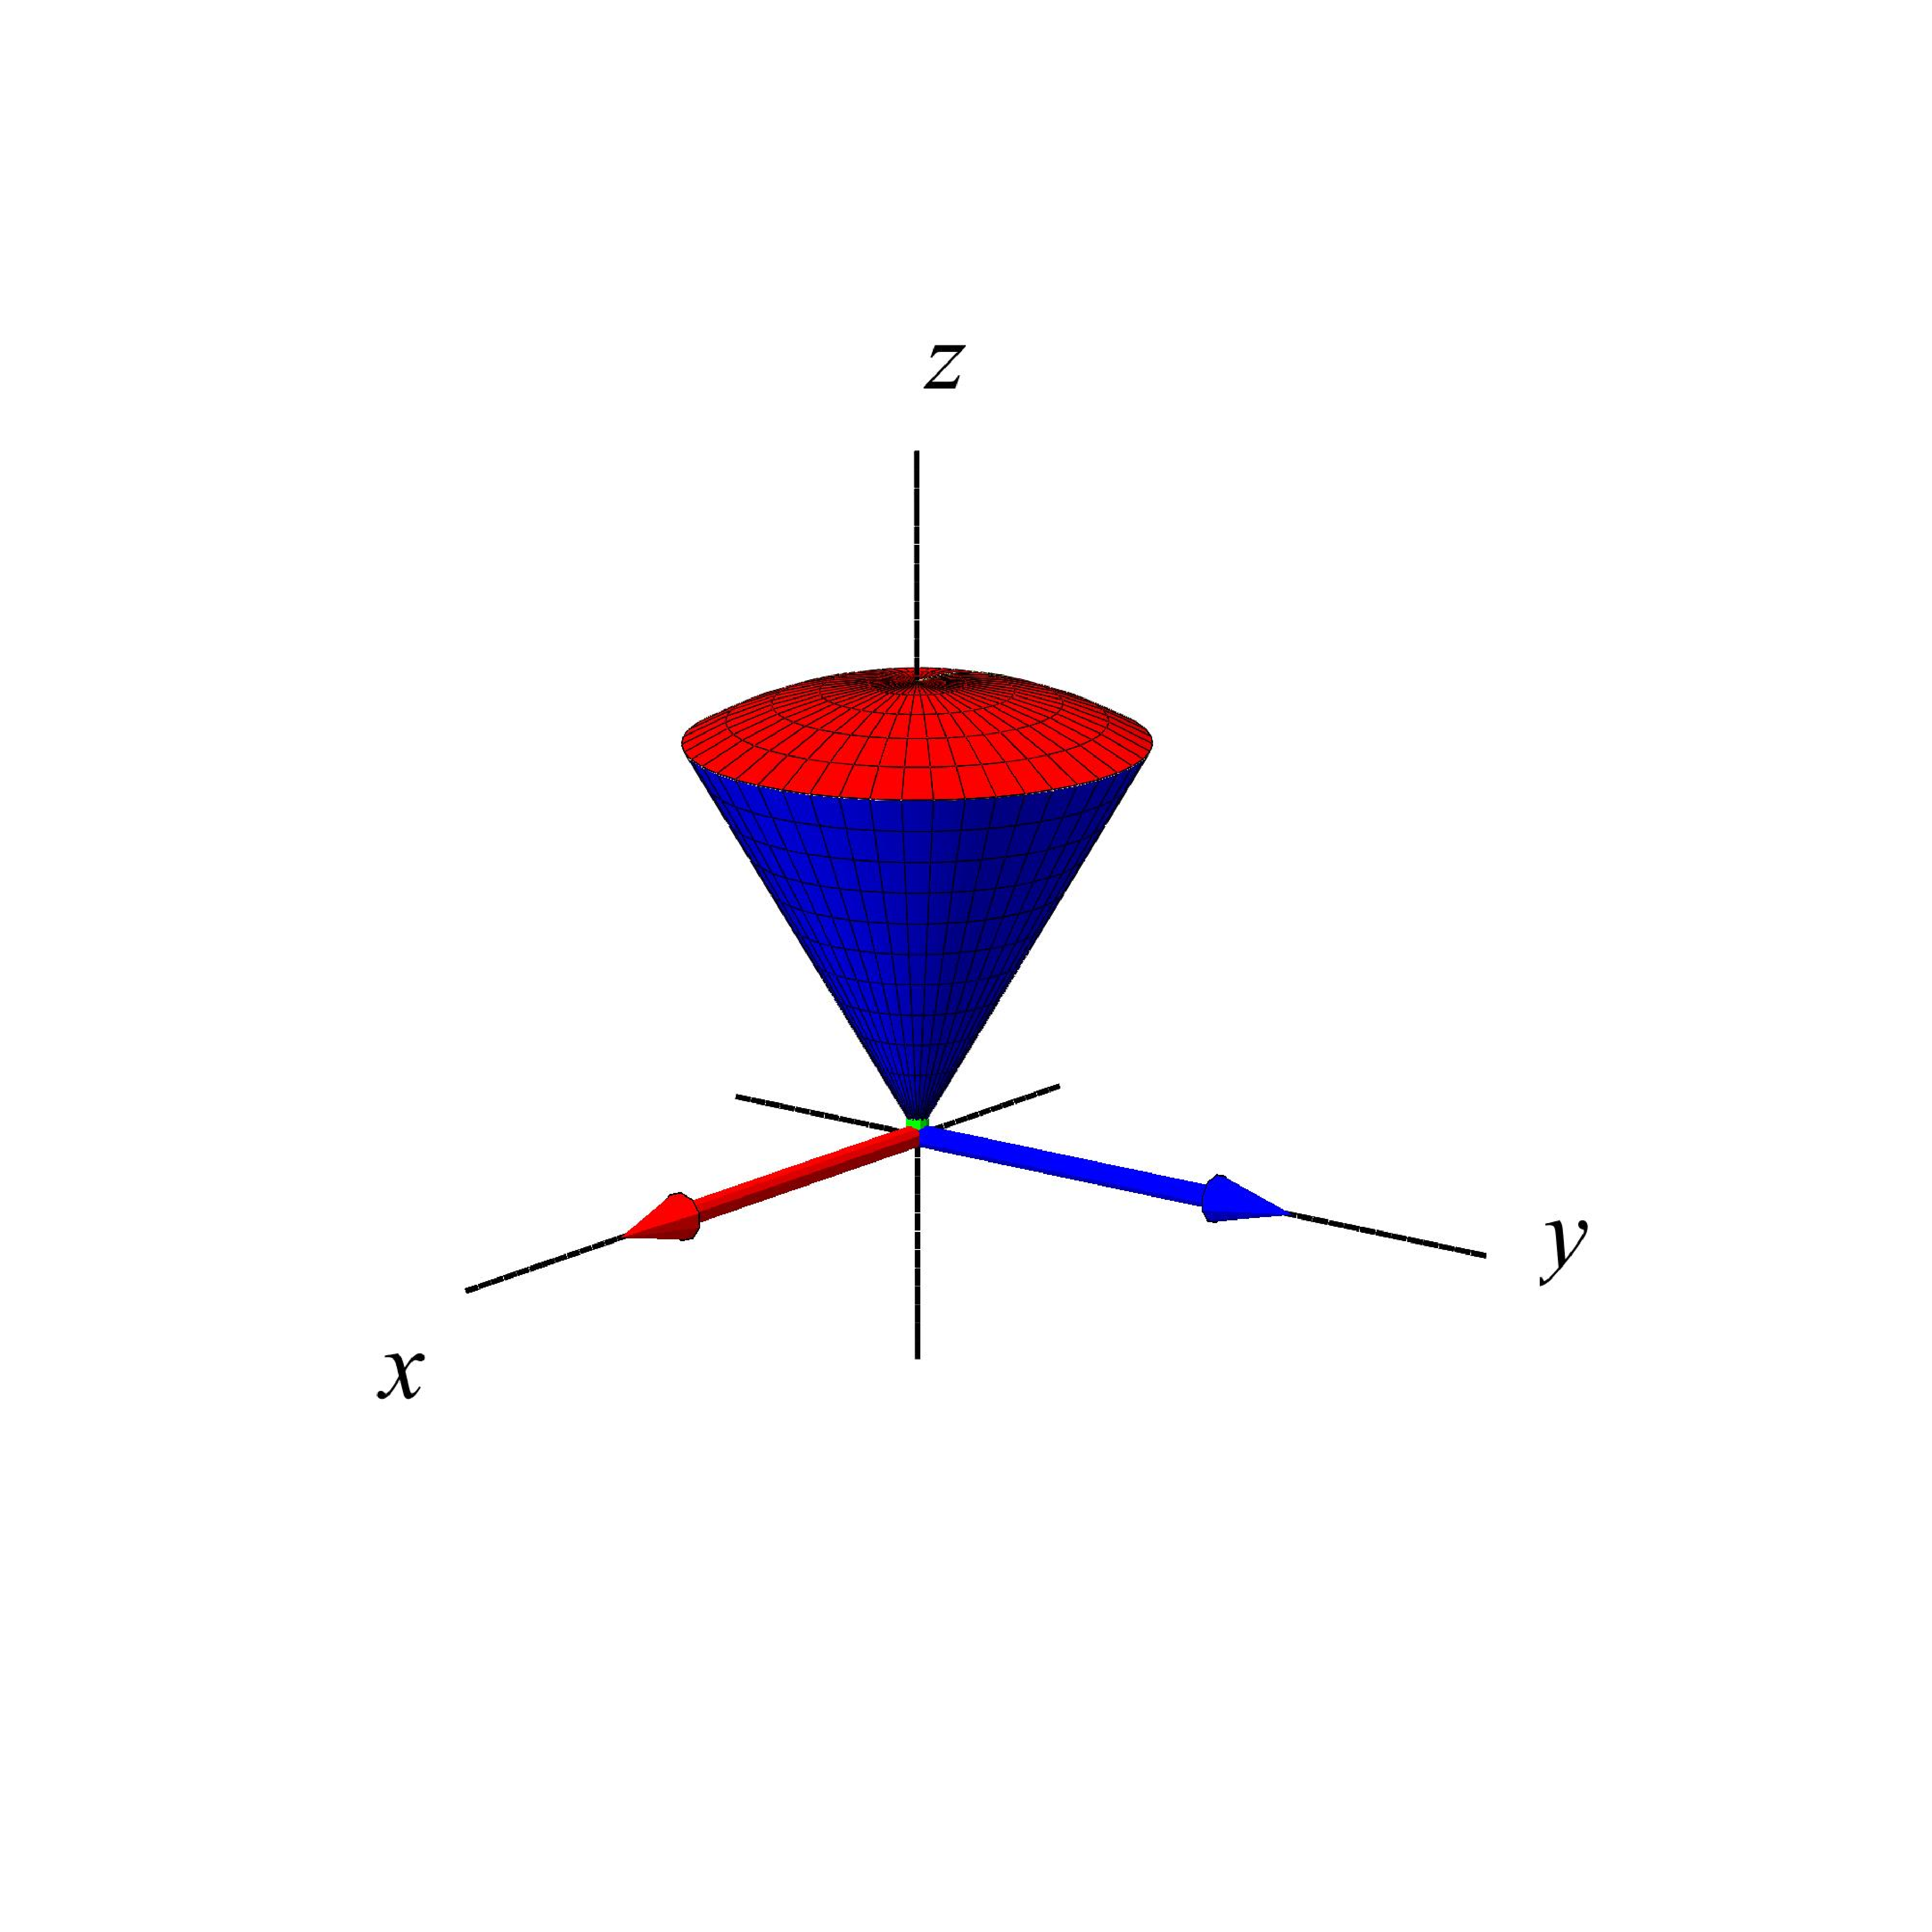
\includegraphics[height=50mm]{FIGS/plotSphereProp1}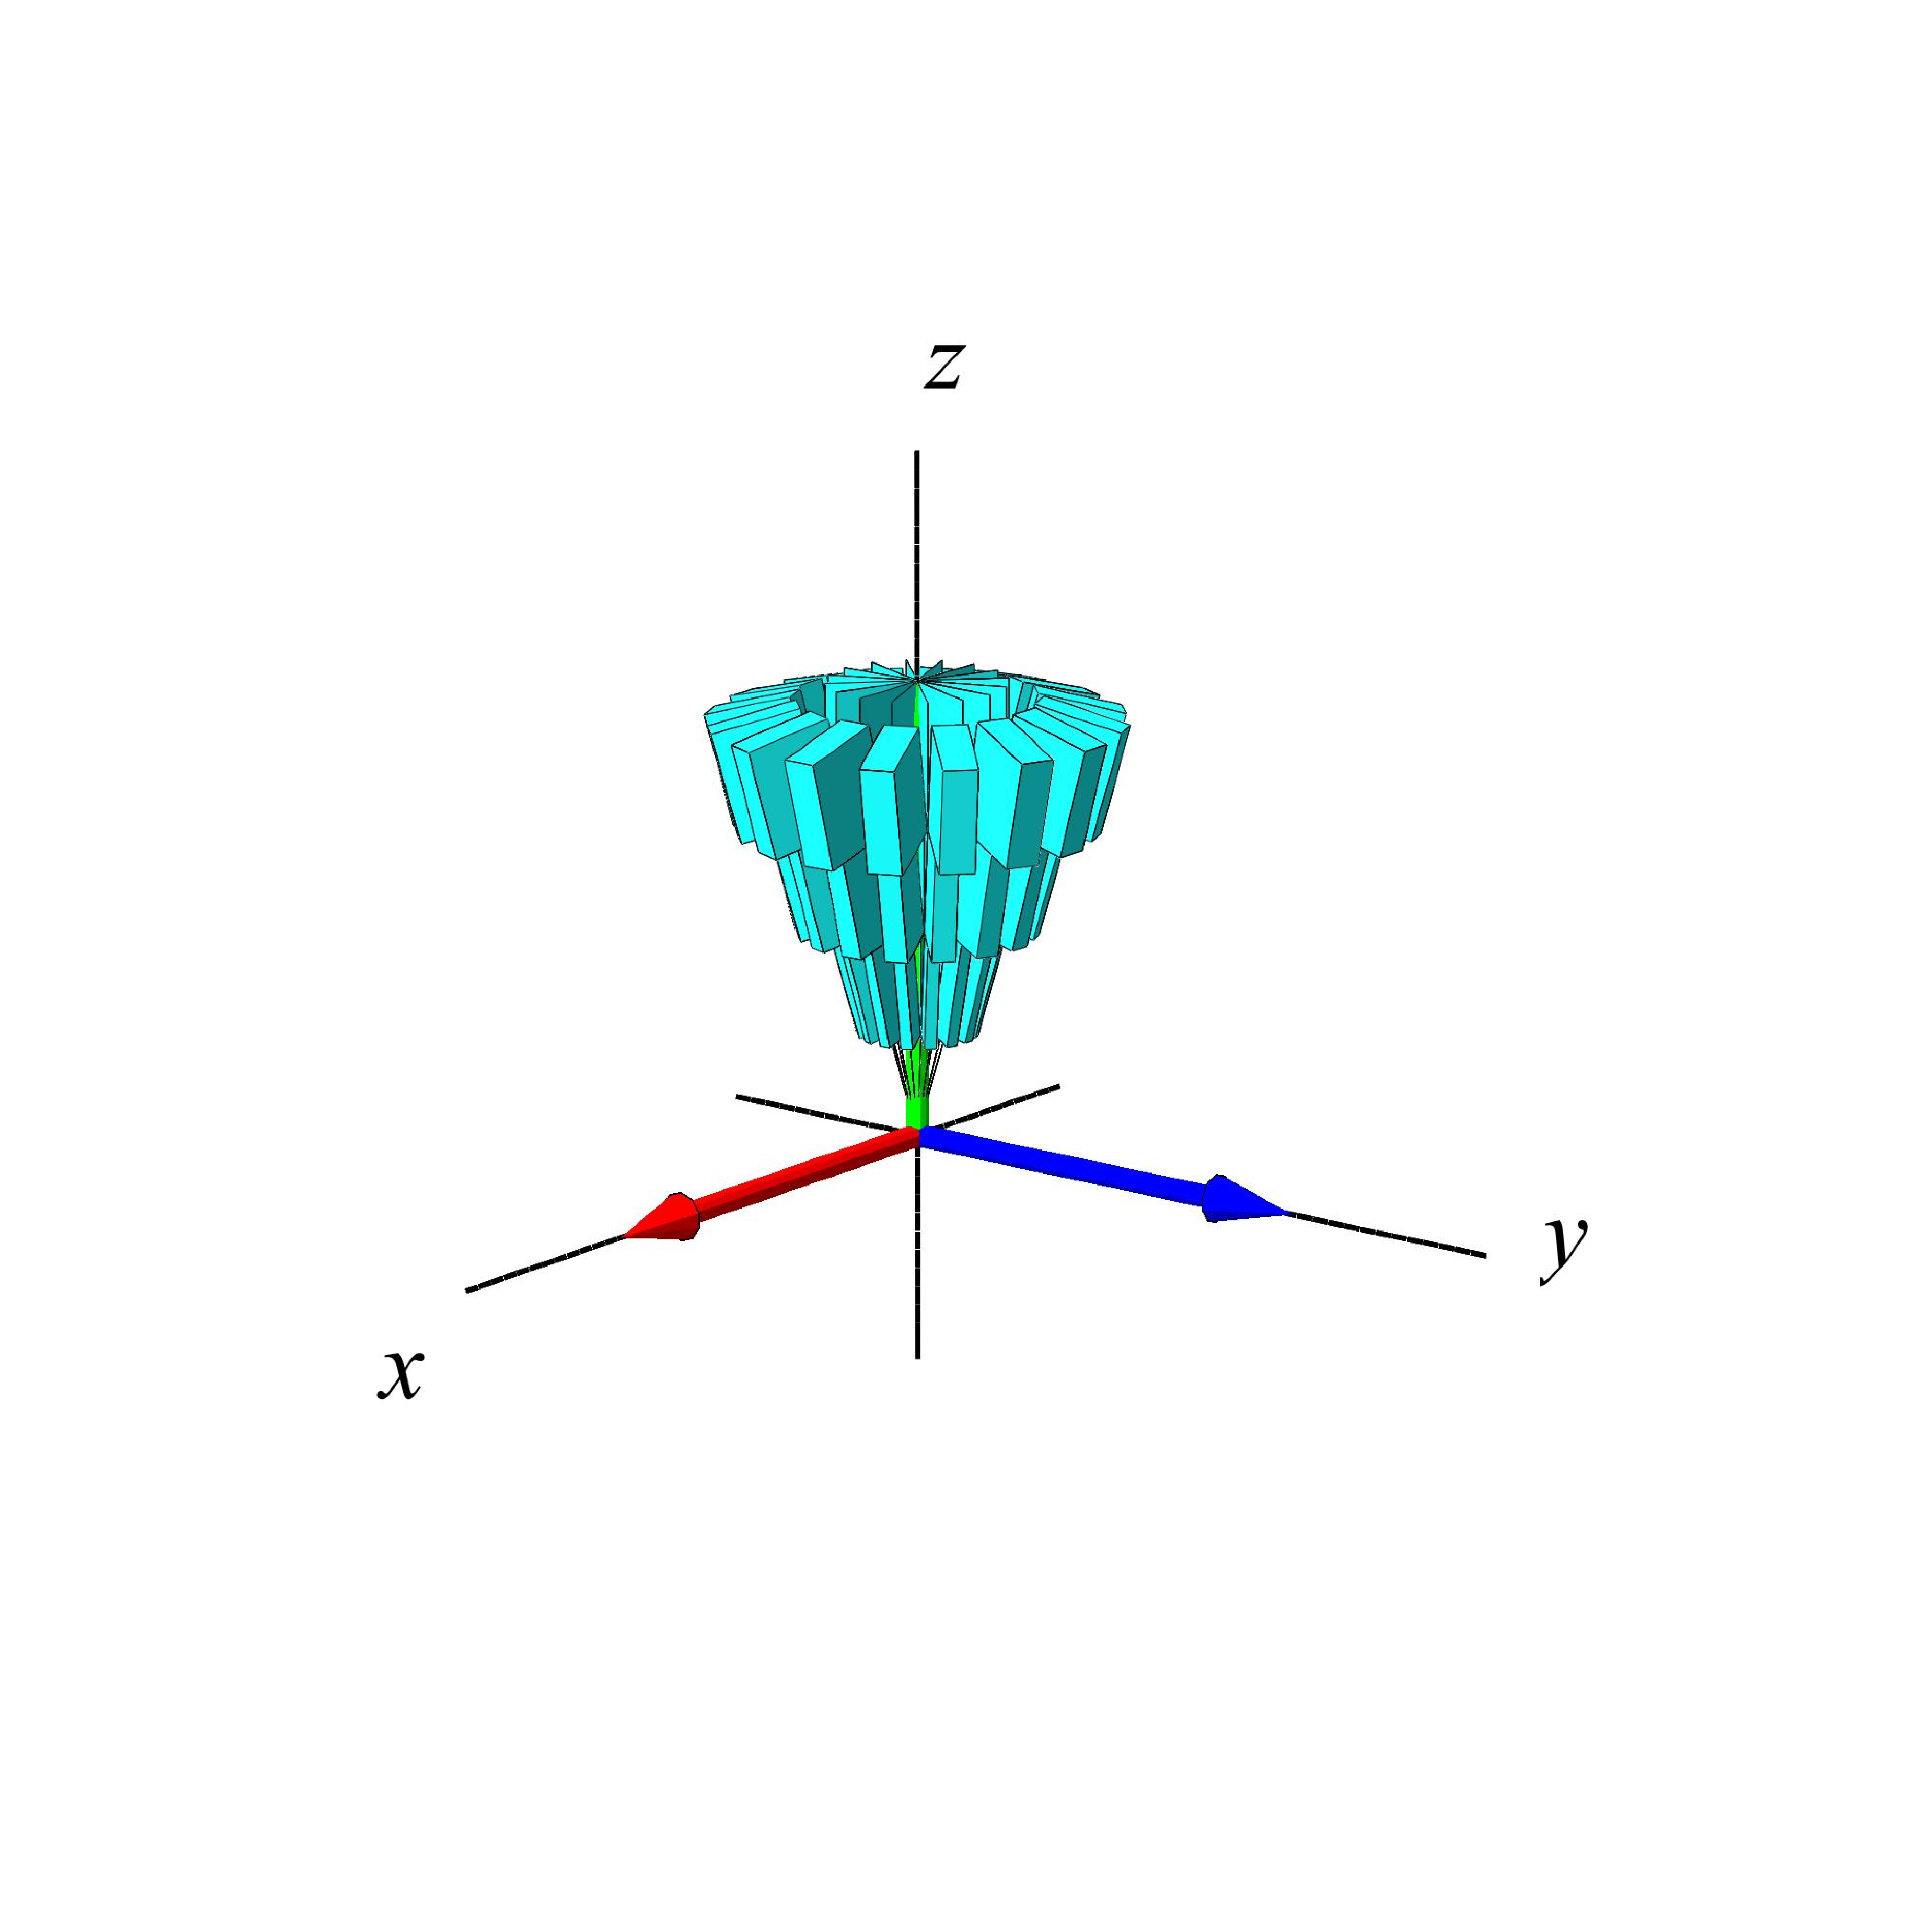
\includegraphics[height=50mm]{FIGS/plotSphereProp3}}
\begin{center}
\caption{\small{Dette {\em rumlige} område er et 'rumvinkel'-udsnit af kuglefladen repræsenteret ved
${\bf r}(u, v, w) \, = \, (u\,\sin(v)\cos(w), u\,\sin(v)\sin(w),
u\,\cos(v) ) \,\,, \,\, u \in [0, 1 ]\,\, , \, \,
v \in [0, \pi/6]\,\, , \, \, w \in [-\pi, \pi]$.}} \label{figKugleProp}
\end{center}
\end{figure}



\begin{example}[Rumfang af massiv ellipsoide] \label{exampEllipRumf}
En massiv {ellipsoide} med halvakser $a$, $b$, og $c$ har en parameterfremstilling:
\begin{equation}
{\bf r}(u, v, w) \, = \, (a\,u\,\sin(v)\cos(w), b\,u\,\sin(v)\sin(w),
c\,u\,\cos(v) ) \quad ,
\end{equation}
hvor $u \in [0,1]$, $ v \in [0,
\pi]$ og $ w \in [-\pi, \pi]$.\\

Jacobi-funktionen for denne parametrisering er $\Jac(u,v,w) \, = \, abc\,u^{2}\,\sin(v)\,$, og deraf følger
volumenet ved tredobbelt integration:
\begin{equation} \label{eqRumintegralVolumen02}
\begin{aligned}
\Vol(\Omega_{\bf r}) \, &= \, \int_{\Omega_{\bf r}} 1 \, d\mu \\ &=
\, \int_{-\pi}^{\pi}\int_{0}^{\pi} \int_{0}^{1} \Jac_{\bf r}(u,v,w)\,du
\, dv \, dw  \\ &= \, abc\,\int_{-\pi}^{\pi}\int_{0}^{\pi} \int_{0}^{1} u^{2}\,\sin(v)\,du
\, dv \, dw \\ &=
\, \frac{4}{3}\pi\,abc \quad .
\end{aligned}
\end{equation}
For en massiv kugle $B_{a}$ med radius $a$ får vi derfor rumfanget
\begin{equation}
\Vol(B_{a}) = \frac{4}{3}\pi\cdot a^{3} \quad .
\end{equation}
\end{example}


\begin{example}[Graf-flade-afgrænset rumligt område]\label{exampGraffladeVol}
En positiv funktion $h(x,y)$ af to variable $(x,y)$ har en grafflade, der over et givet område $P$ i $(x,y)$-planen
afgrænser et rumligt område. Det er let at parametrisere det rumlige område, når først det plane område er parametriseret.\\

Hvis det plane område er givet ved et rektangel $(x,y) \in [a,b]\times[c, d]$ har vi parameterfremstillingen for det rumlige område:
\begin{equation}
\Omega_{\mathbf{r}} \quad : \quad \mathbf{r}(u,v,w) = (u, v, w\cdot h(u,v)) \quad , \quad (u,v) \in [a,b]\times[c, d] \quad , \quad w \in [0, 1]\quad .
\end{equation}
Jacobifunktionen er særlig simpel:
\begin{equation}
\begin{aligned}
\Jac_{\mathbf{r}}(u,v,w) &= | ((1,0, w\cdot h'_{u}(u,v)) \times (0,1, w\cdot h'_{v}(u,v))) \bm{\cdot} (0,0,h(u,v)) | \\
& = | ((1,0, *) \times (0,1, **)) \bm{\cdot} (0,0,h(u,v)) |  \\
&= h(u,v) \quad.
\end{aligned}
\end{equation}
Rumfanget af det rumlig område, som graf-fladen afgrænser sammen med det plane område i $(x,y)$-planen er derfor:
\begin{equation}
\Vol(\Omega_{\mathbf{r}}) =
\, \int_{0}^{1}\int_{c}^{d} \int_{a}^{b} h(u,v) \,du
\, dv \, dw = \int_{c}^{d} \int_{a}^{b} h(u,v) \,du
\, dv \quad .
\end{equation}

Hvis det plane område $P$ i $(x,y)$-planen ikke er et rektangel som ovenfor, må vi først pa\-ra\-me\-tri\-se\-re $P$. Vi antager derfor nu, at det plane område $P$ er billedet af
et rektangulært parameterområde ved en vektorfunktion $\widehat{\mathbf{r}}$:
\begin{equation}
P \quad : \quad \widehat{\mathbf{r}}(u,v) = (\xi(u,v), \eta(u,v)) \quad , u \in [a, b] \quad , \quad v \in [c, d] \quad ,
\end{equation}
hvor $\xi(u,v)$ og $\eta(u,v)$ er givne funktioner af $u$ og $v$. Så er det rumlige område imellem $P$ og graffladen for $h(x,y)$ givet ved parameterfremstillingen:
\begin{equation}
\Omega_{\mathbf{r}} \quad : \quad \mathbf{r}(u,v,w) = (\xi(u,v), \eta(u,v), w\cdot h(\xi(u,v),\eta(u,v))) \quad ,
\end{equation}
hvor $(u,v) \in [a,b]\times[c, d]$ og $w \in [0, 1]$
med tilhørende Jacobi-funktion:
\begin{equation}
\begin{aligned}
&\Jac_{\mathbf{r}}(u,v,w) = \\
& = |((\xi'_{u}(u,v),\eta'_{u}(u,v), *) \times (\xi'_{v}(u,v),\eta'_{v}(u,v), **)) \bm{\cdot} (0,0,h(\xi(u,v),\eta(u,v)))  |  \\
&= h(\xi(u,v),\eta(u,v))\cdot \Jac_{\widehat{\mathbf{r}}}(u,v) \quad.
\end{aligned}
\end{equation}
Rumfanget af det rumlig område, som graf-fladen afgrænser sammen med det plane område i $(x,y)$-planen er derfor i denne mere generelle situation:
\begin{equation}
\begin{aligned}
\Vol(\Omega_{\mathbf{r}}) &=
\, \int_{0}^{1}\int_{c}^{d} \int_{a}^{b} h(\xi(u,v),\eta(u,v))\cdot \Jac_{\widehat{\mathbf{r}}}(u,v)  \,du
\, dv \, dw \\
&= \int_{c}^{d} \int_{a}^{b} h(\xi(u,v),\eta(u,v))\cdot \Jac_{\widehat{\mathbf{r}}}(u,v)  \,du
\, dv \quad .
\end{aligned}
\end{equation}
\end{example}

\begin{figure}[h]
\centerline{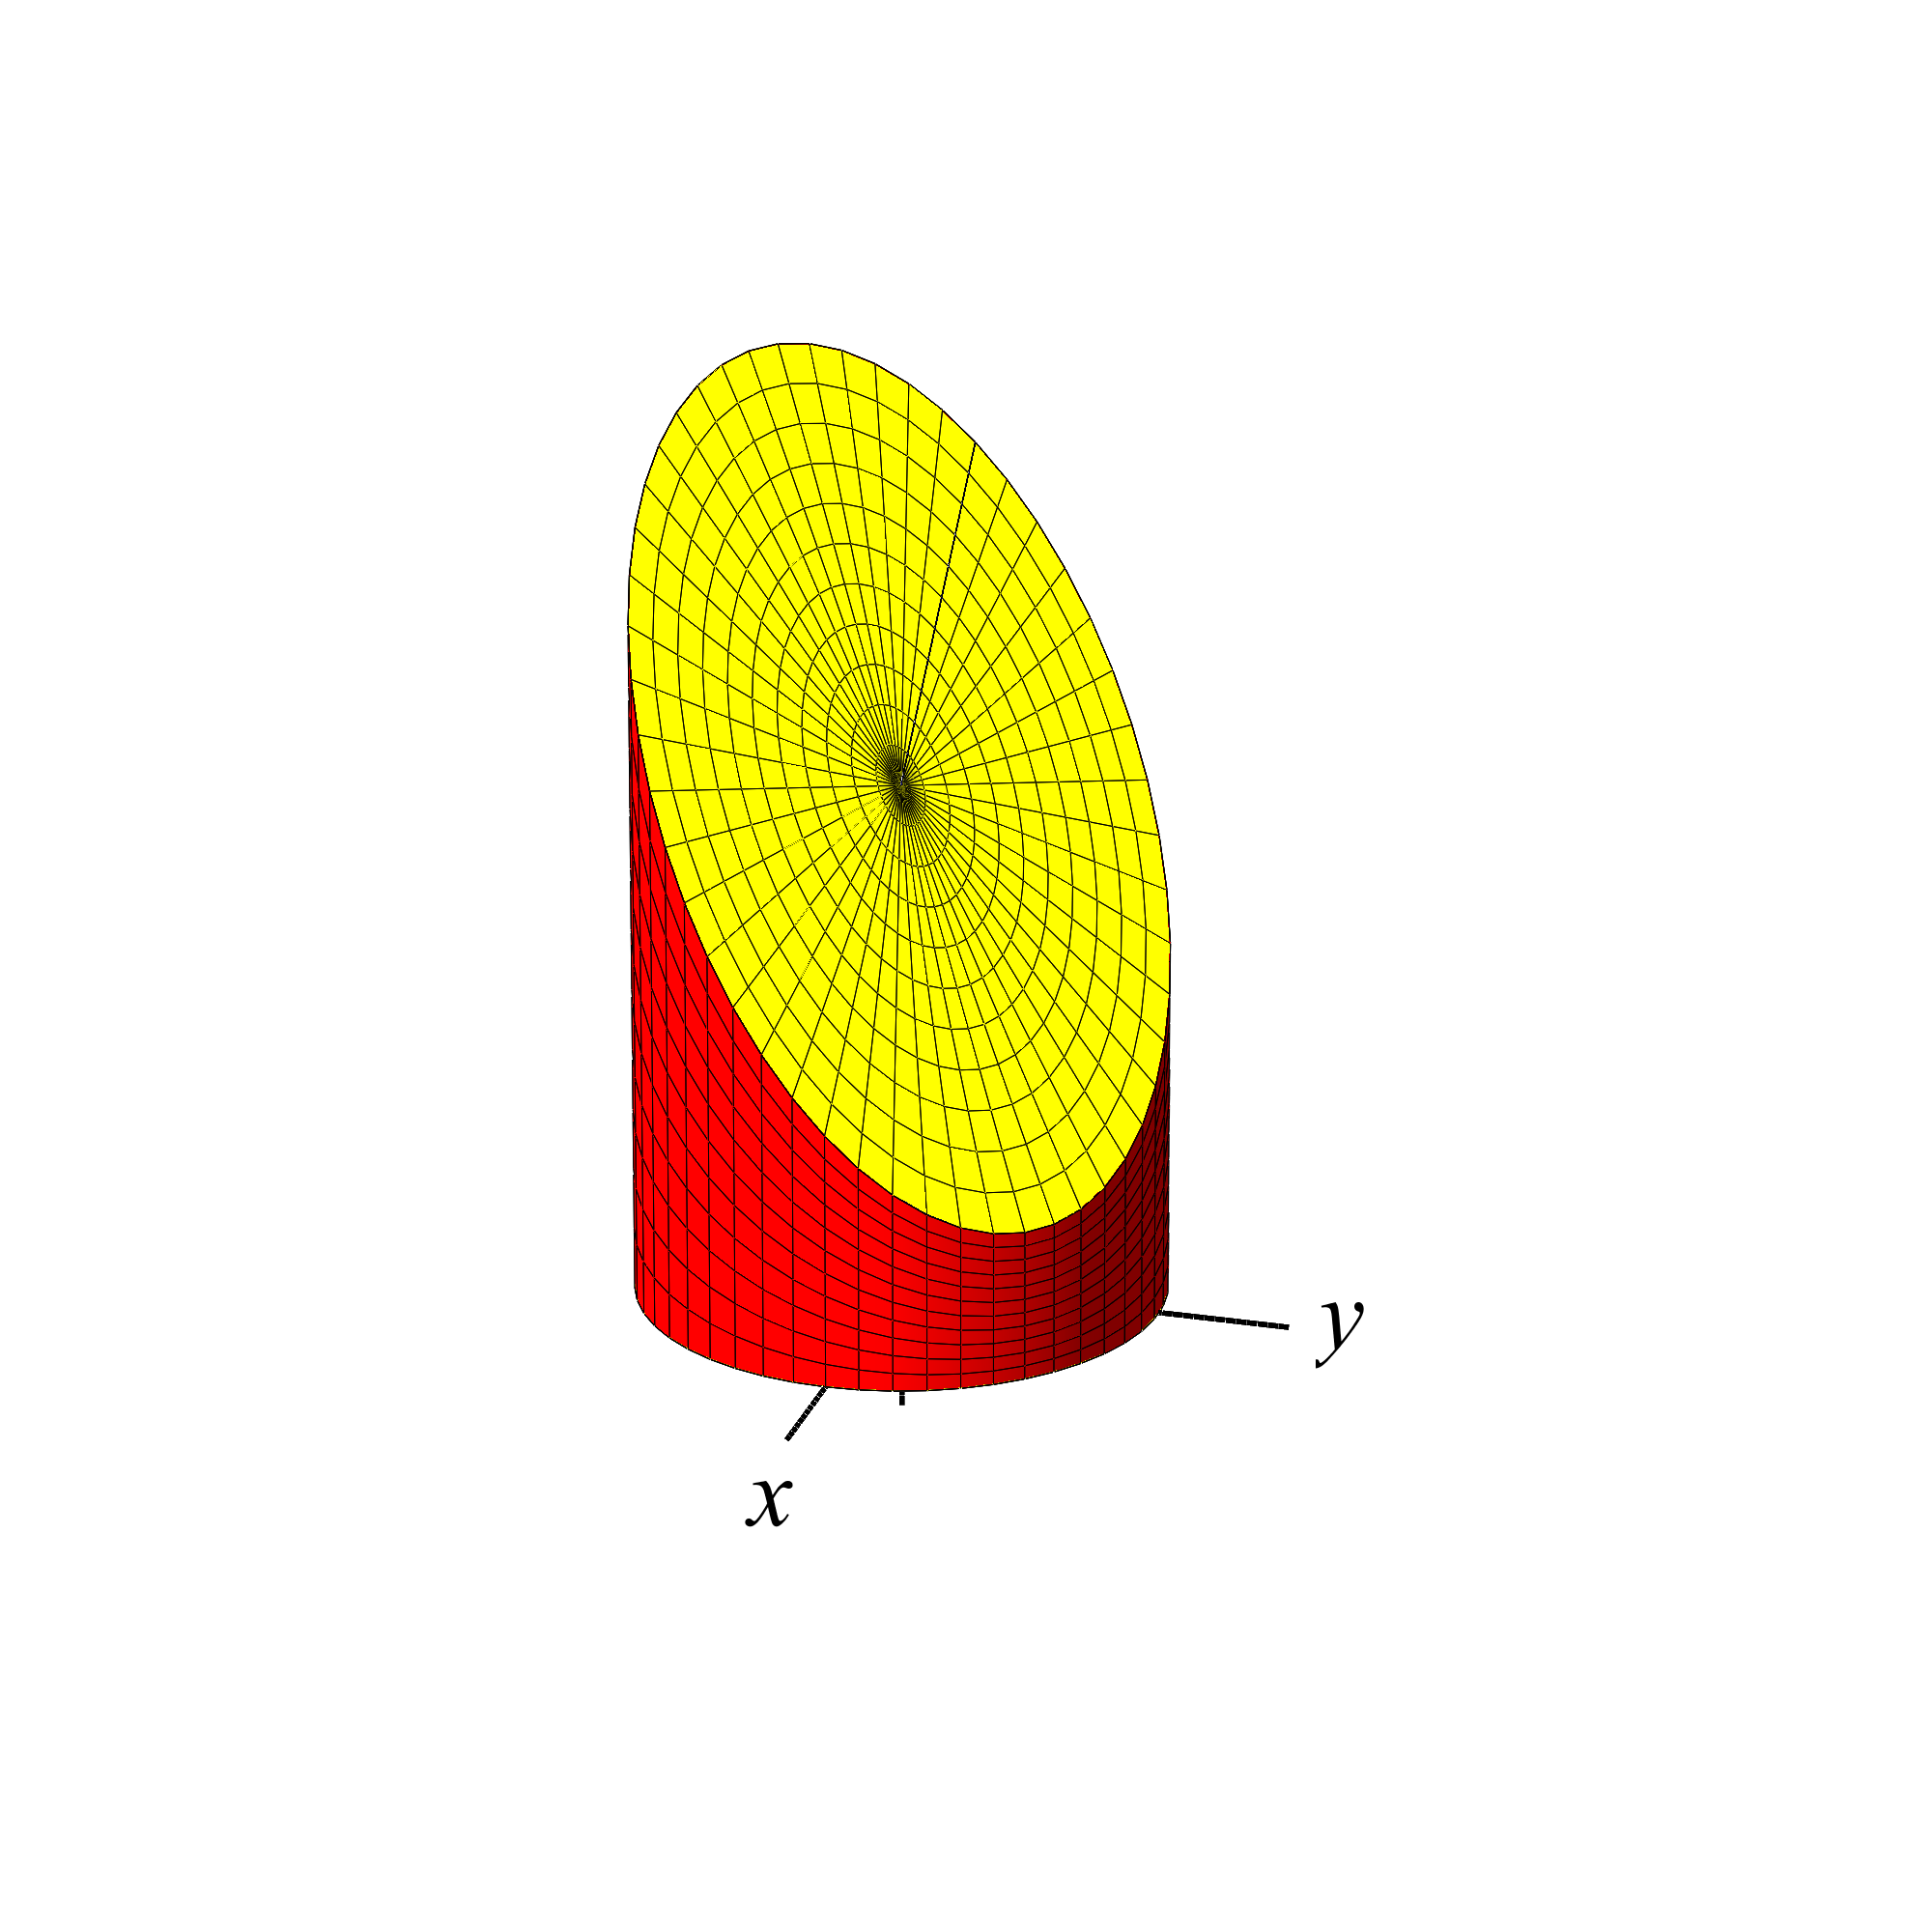
\includegraphics[height=70mm]{FIGS/plotGrafVol1} 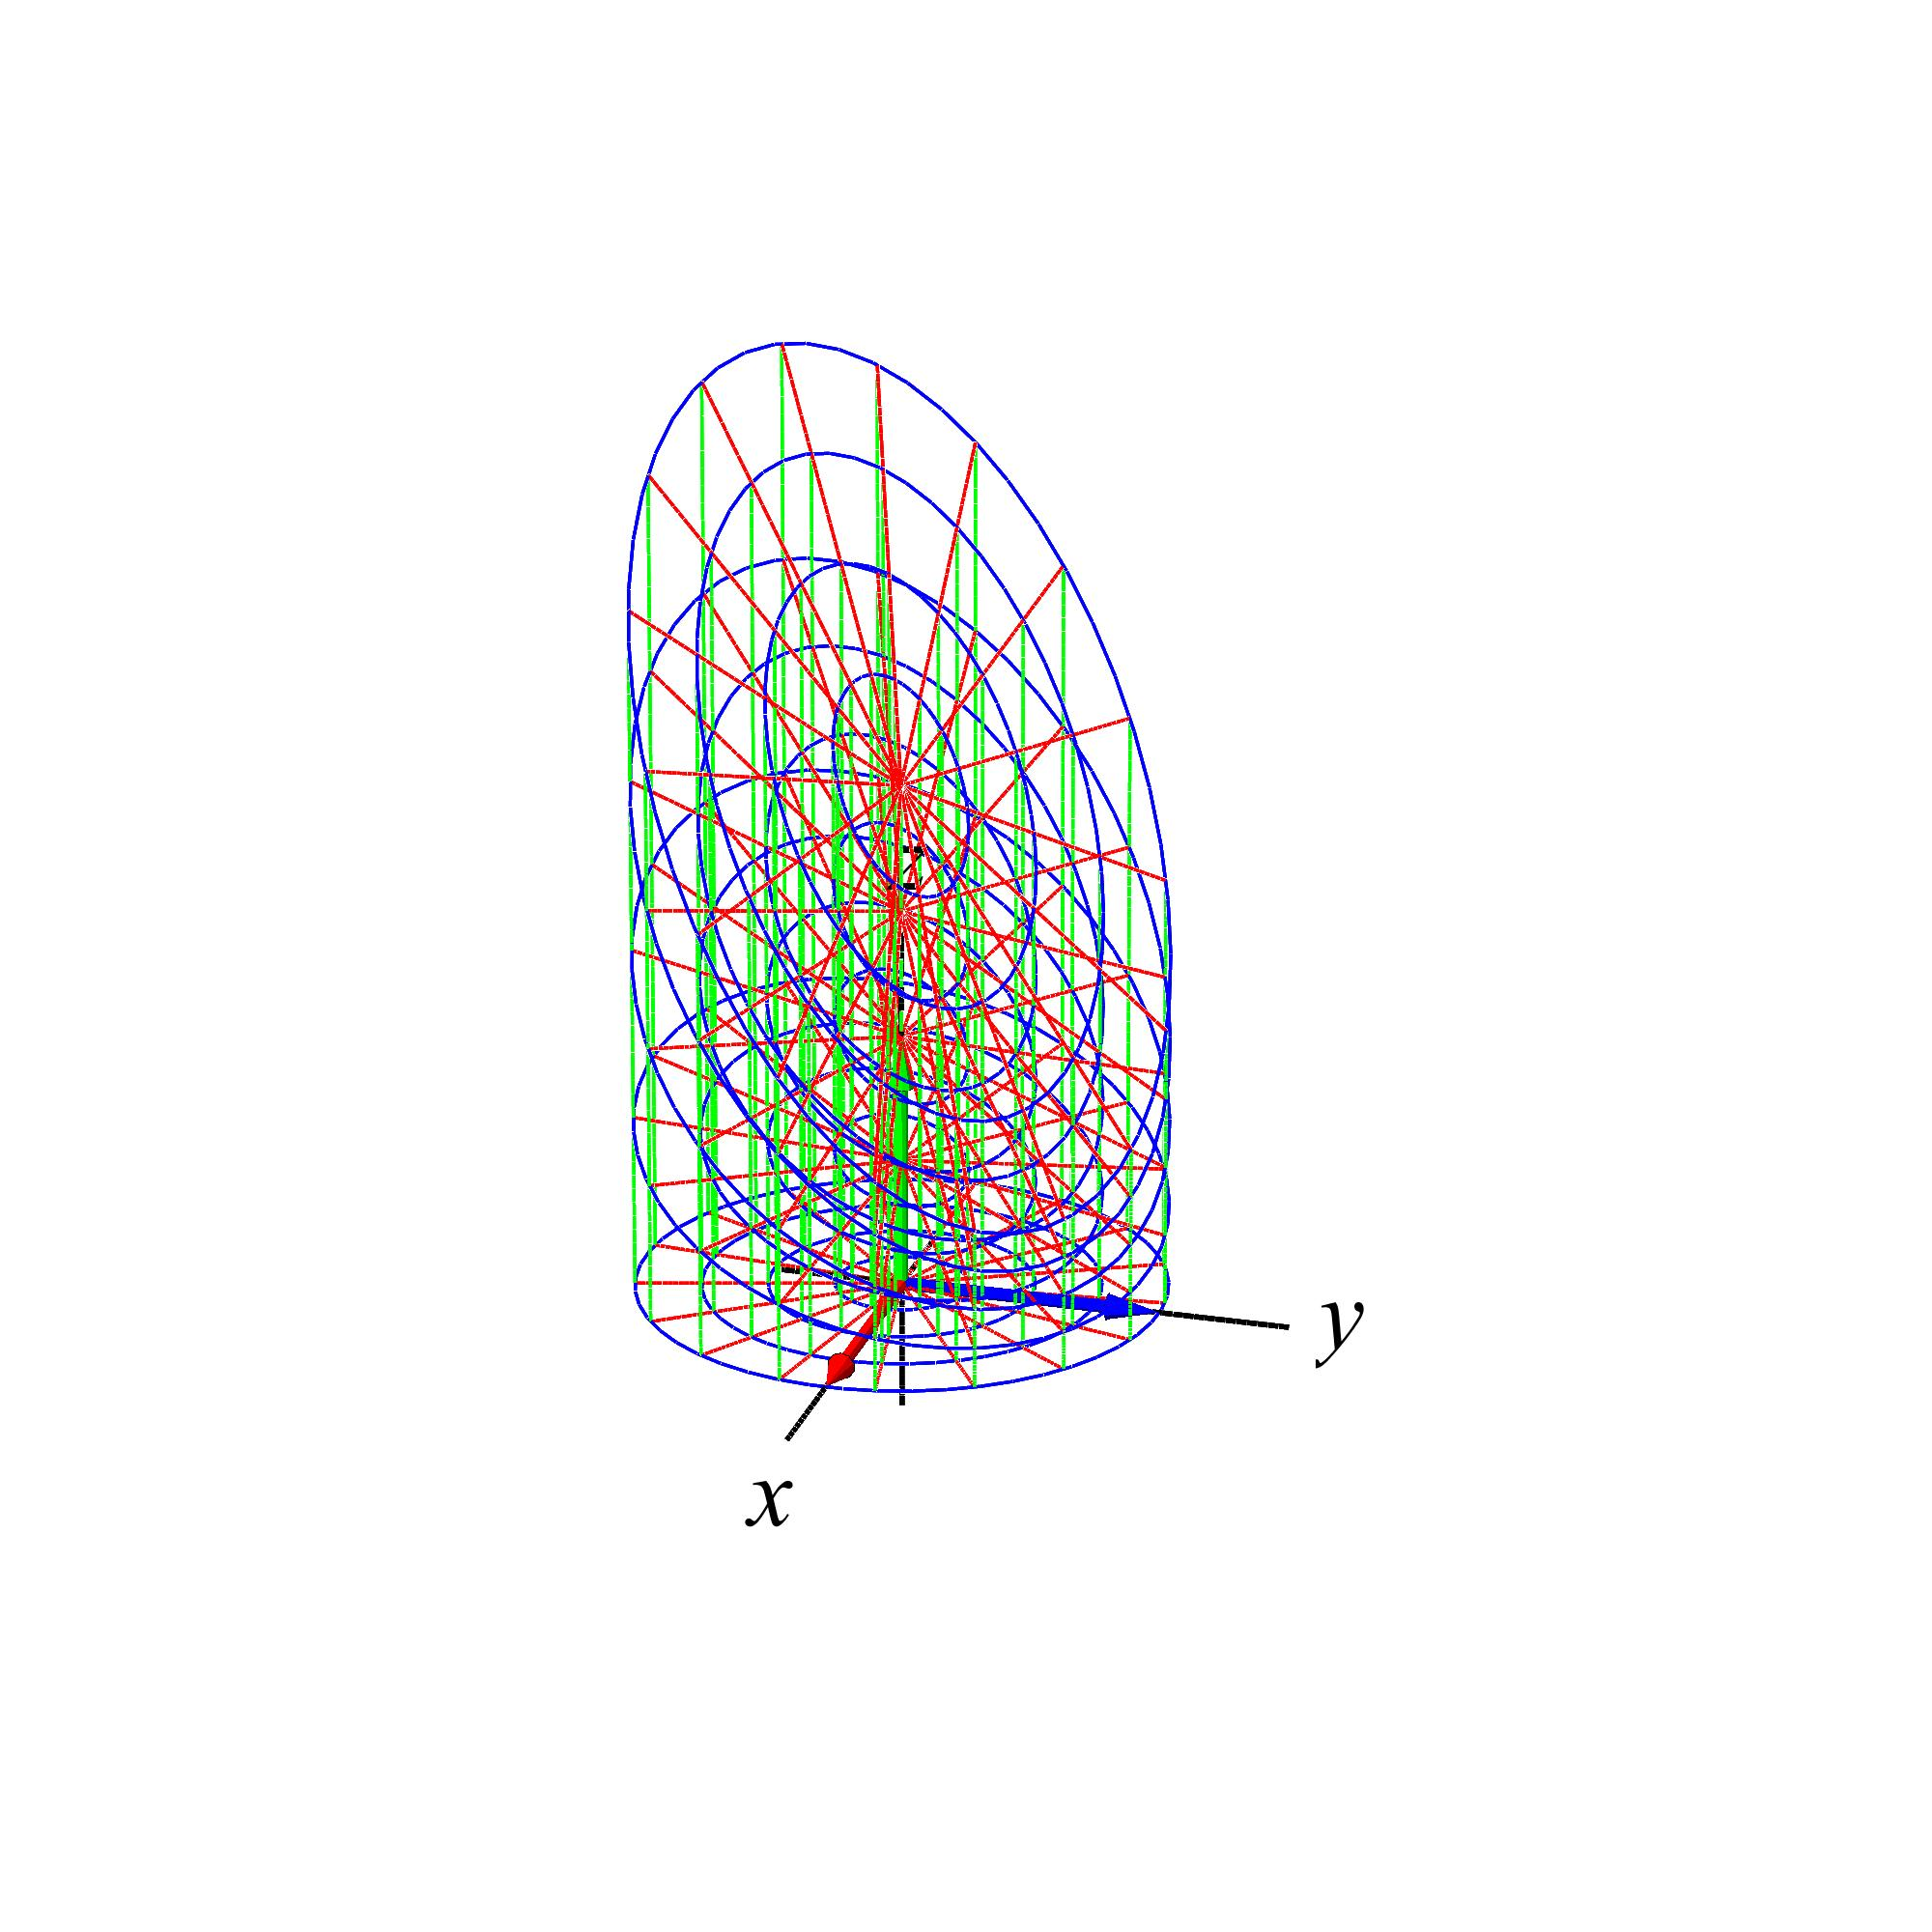
\includegraphics[height=70mm]{FIGS/plotGrafVol2} 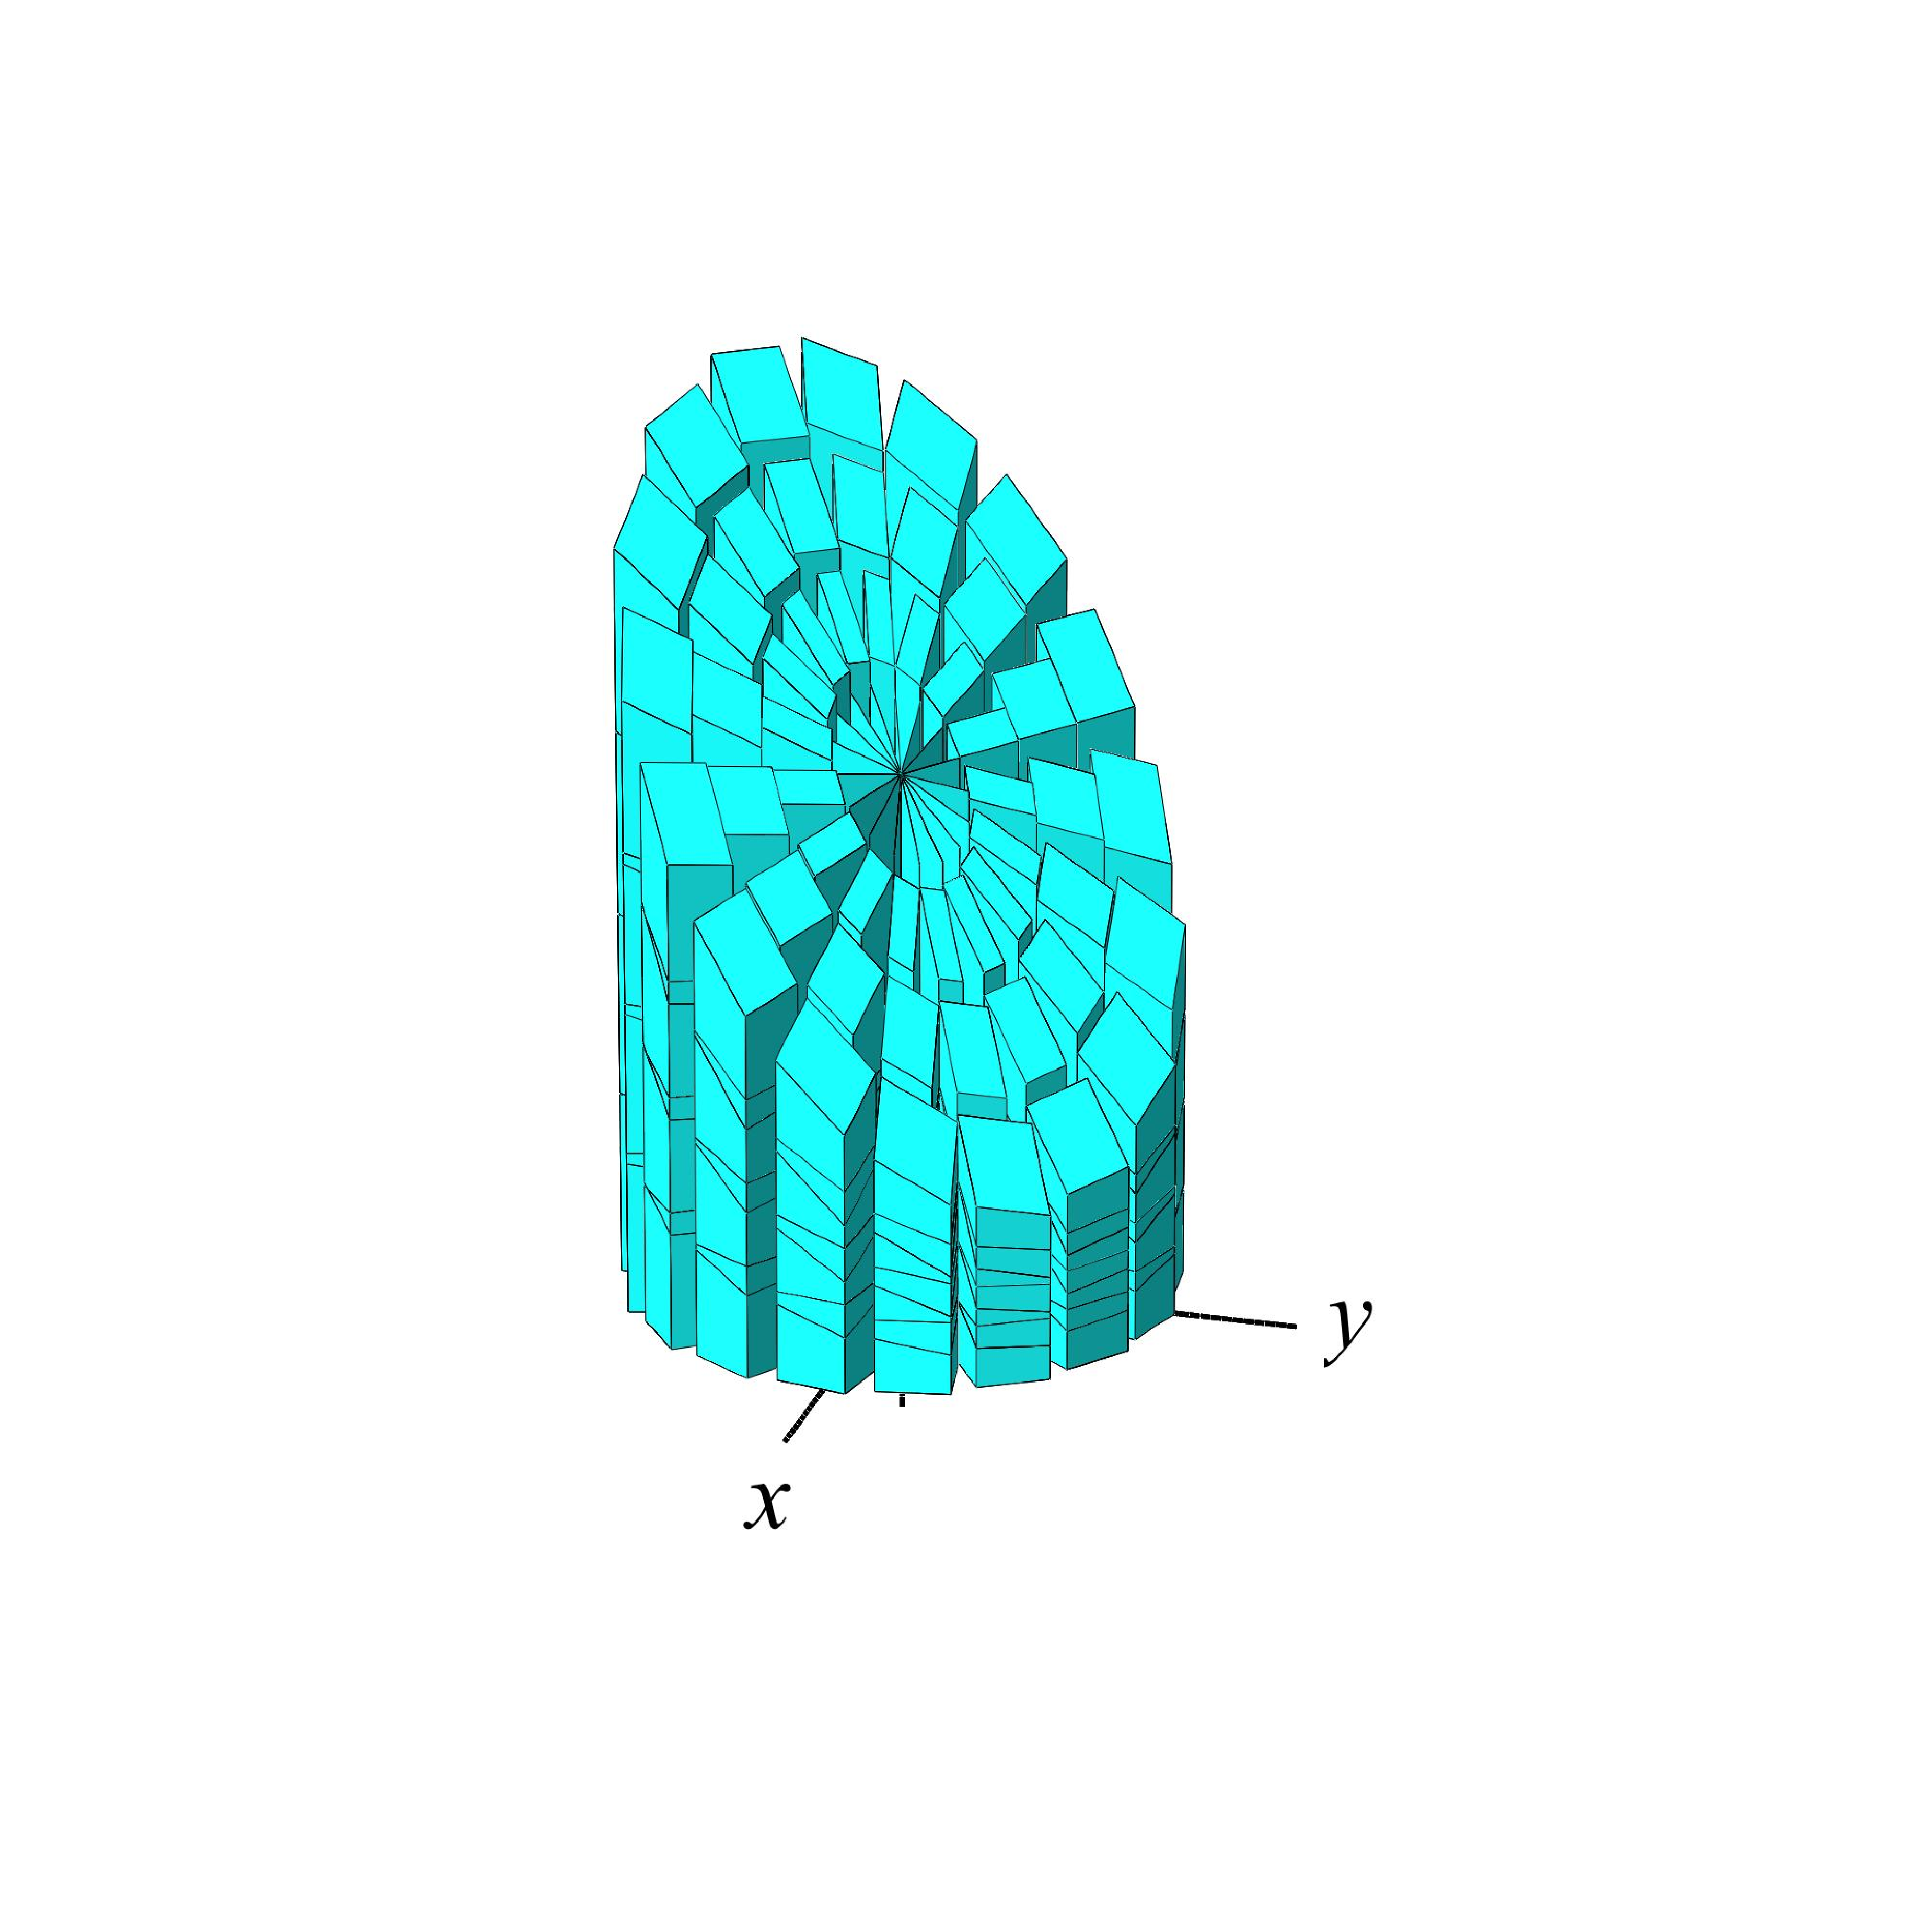
\includegraphics[height=70mm]{FIGS/plotGrafVol3}}
\begin{center}
\caption{\small{Planetariet er afgrænset af graffladen for $f(x,y)= 2-x-y$ over en cirkulær grundplan i $(x,y)$-planen med radius $1$ og centrum i $(0,0)$. Rumfanget er $2\pi$.}}
\label{figGrafVol}
\end{center}
\end{figure}

\begin{figure}[h]
\centerline{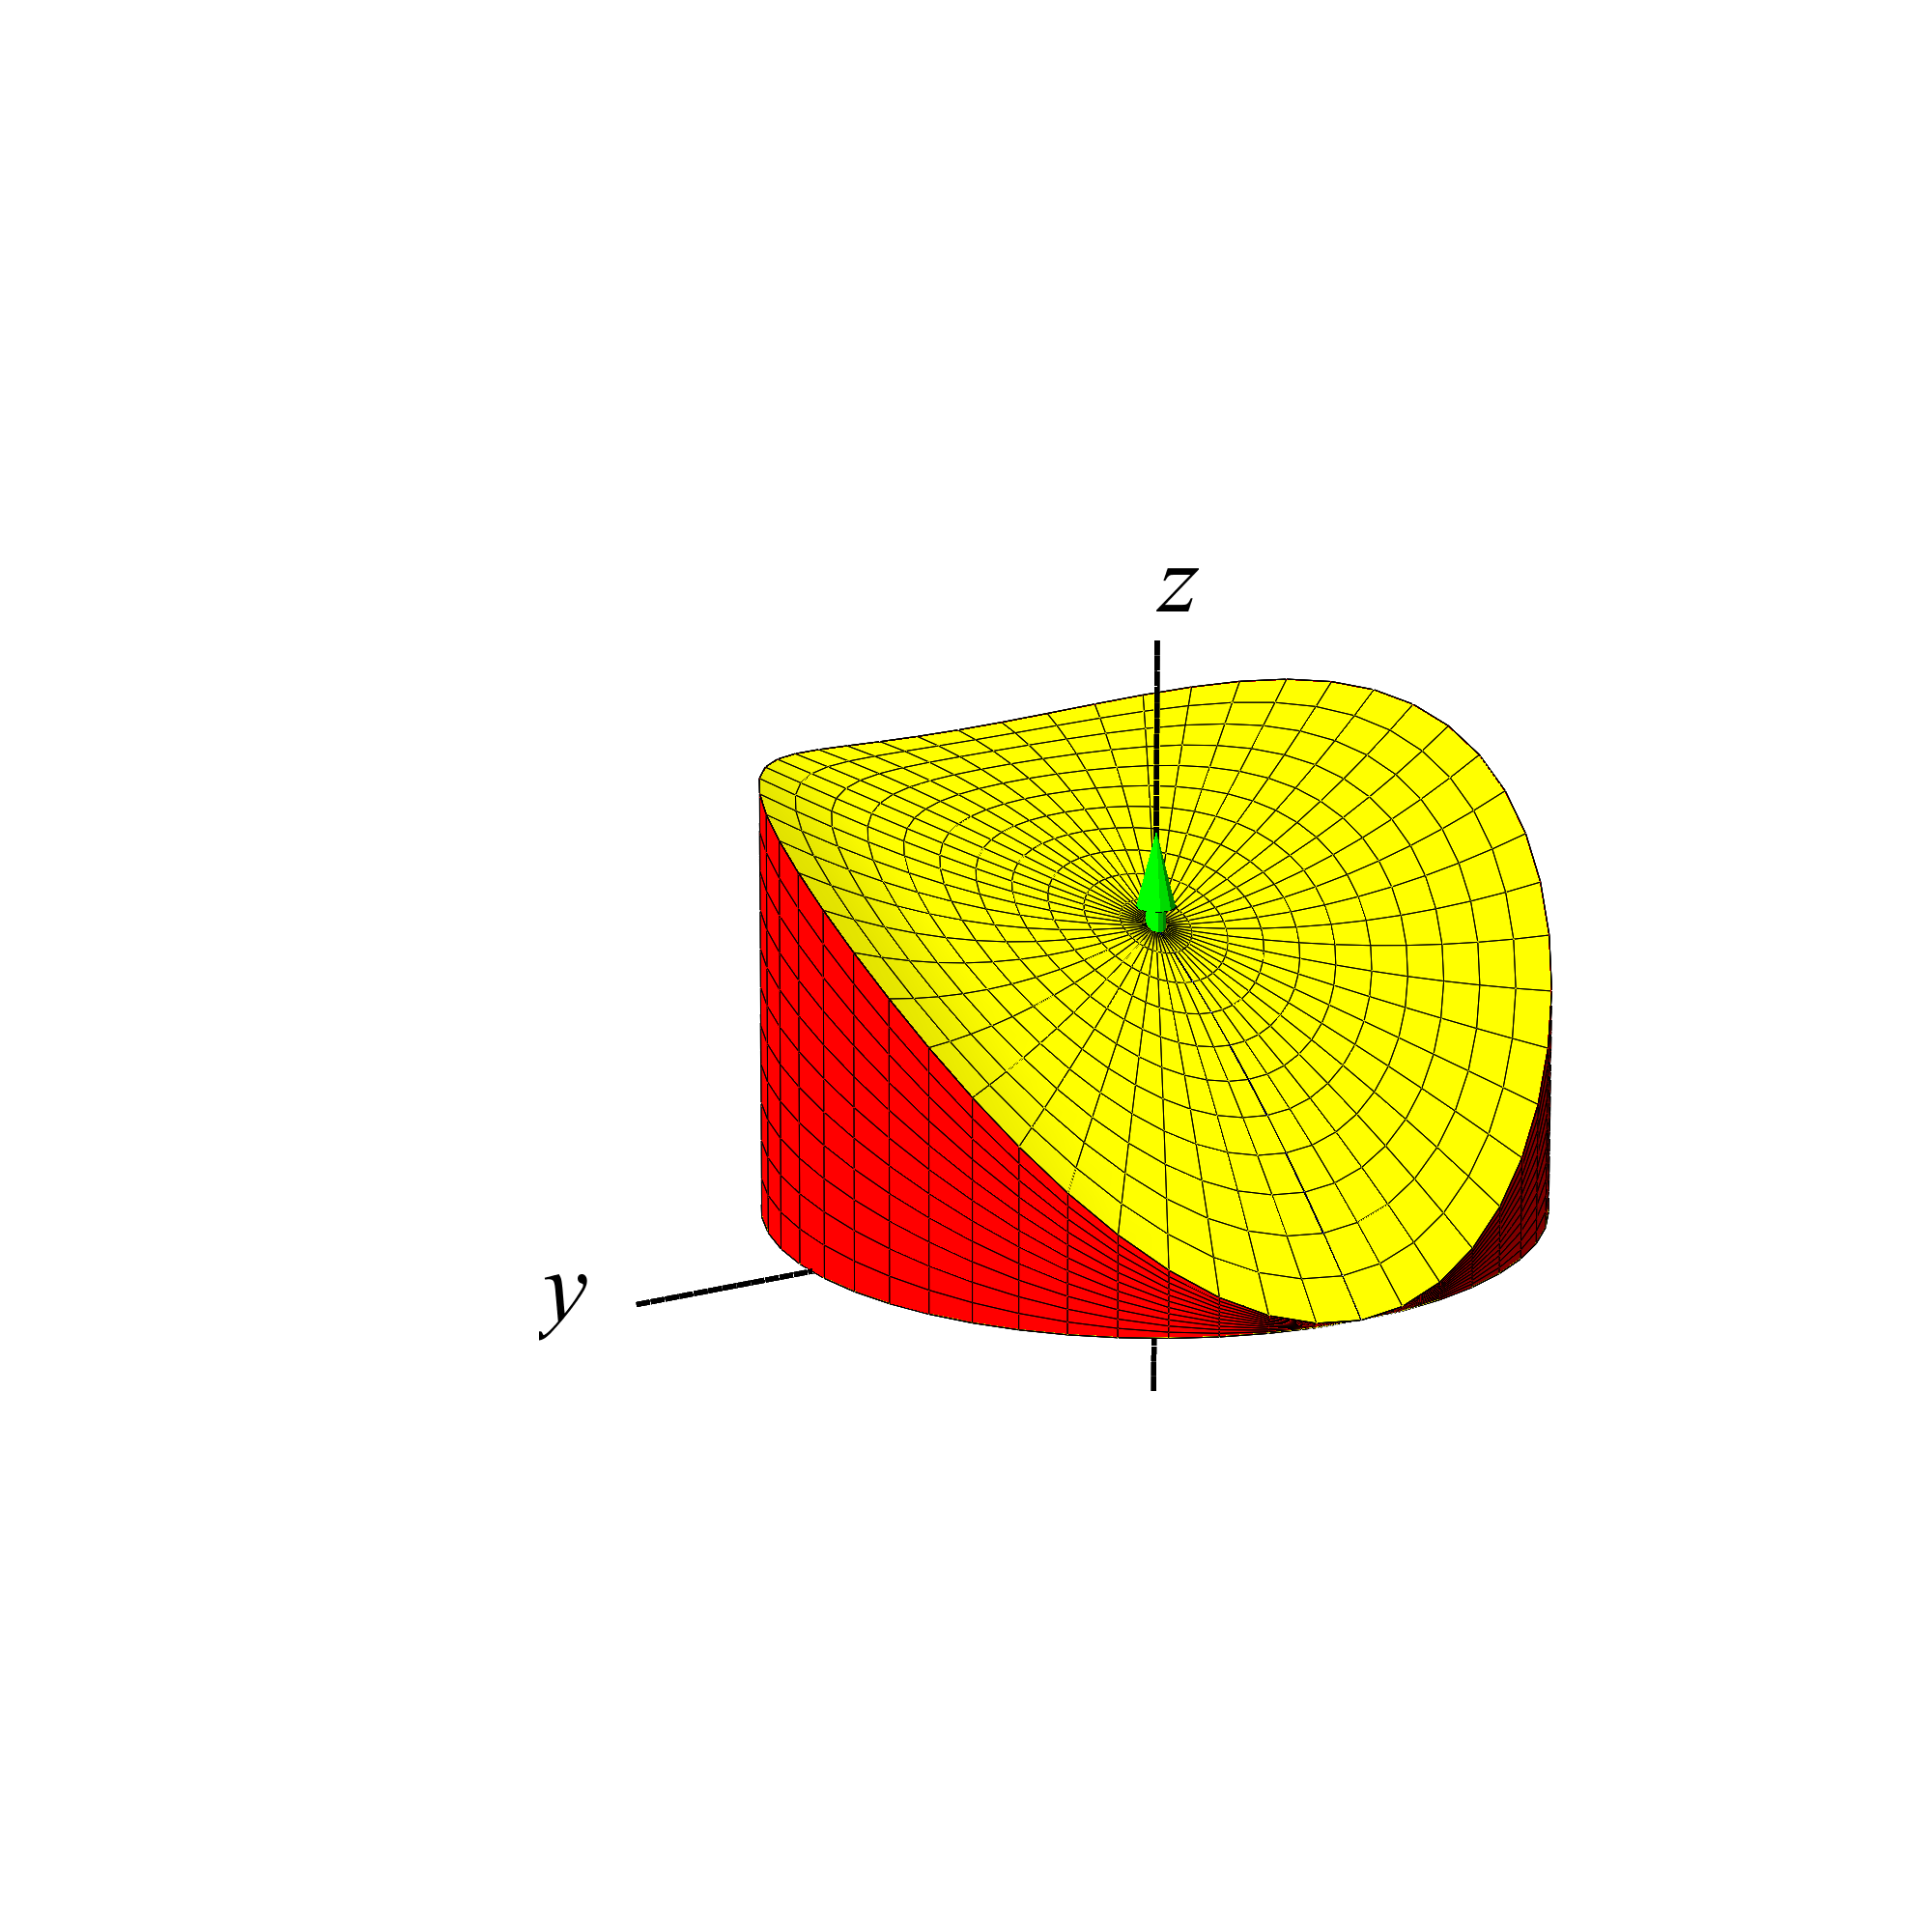
\includegraphics[height=70mm]{FIGS/plotGrafHypVol1} 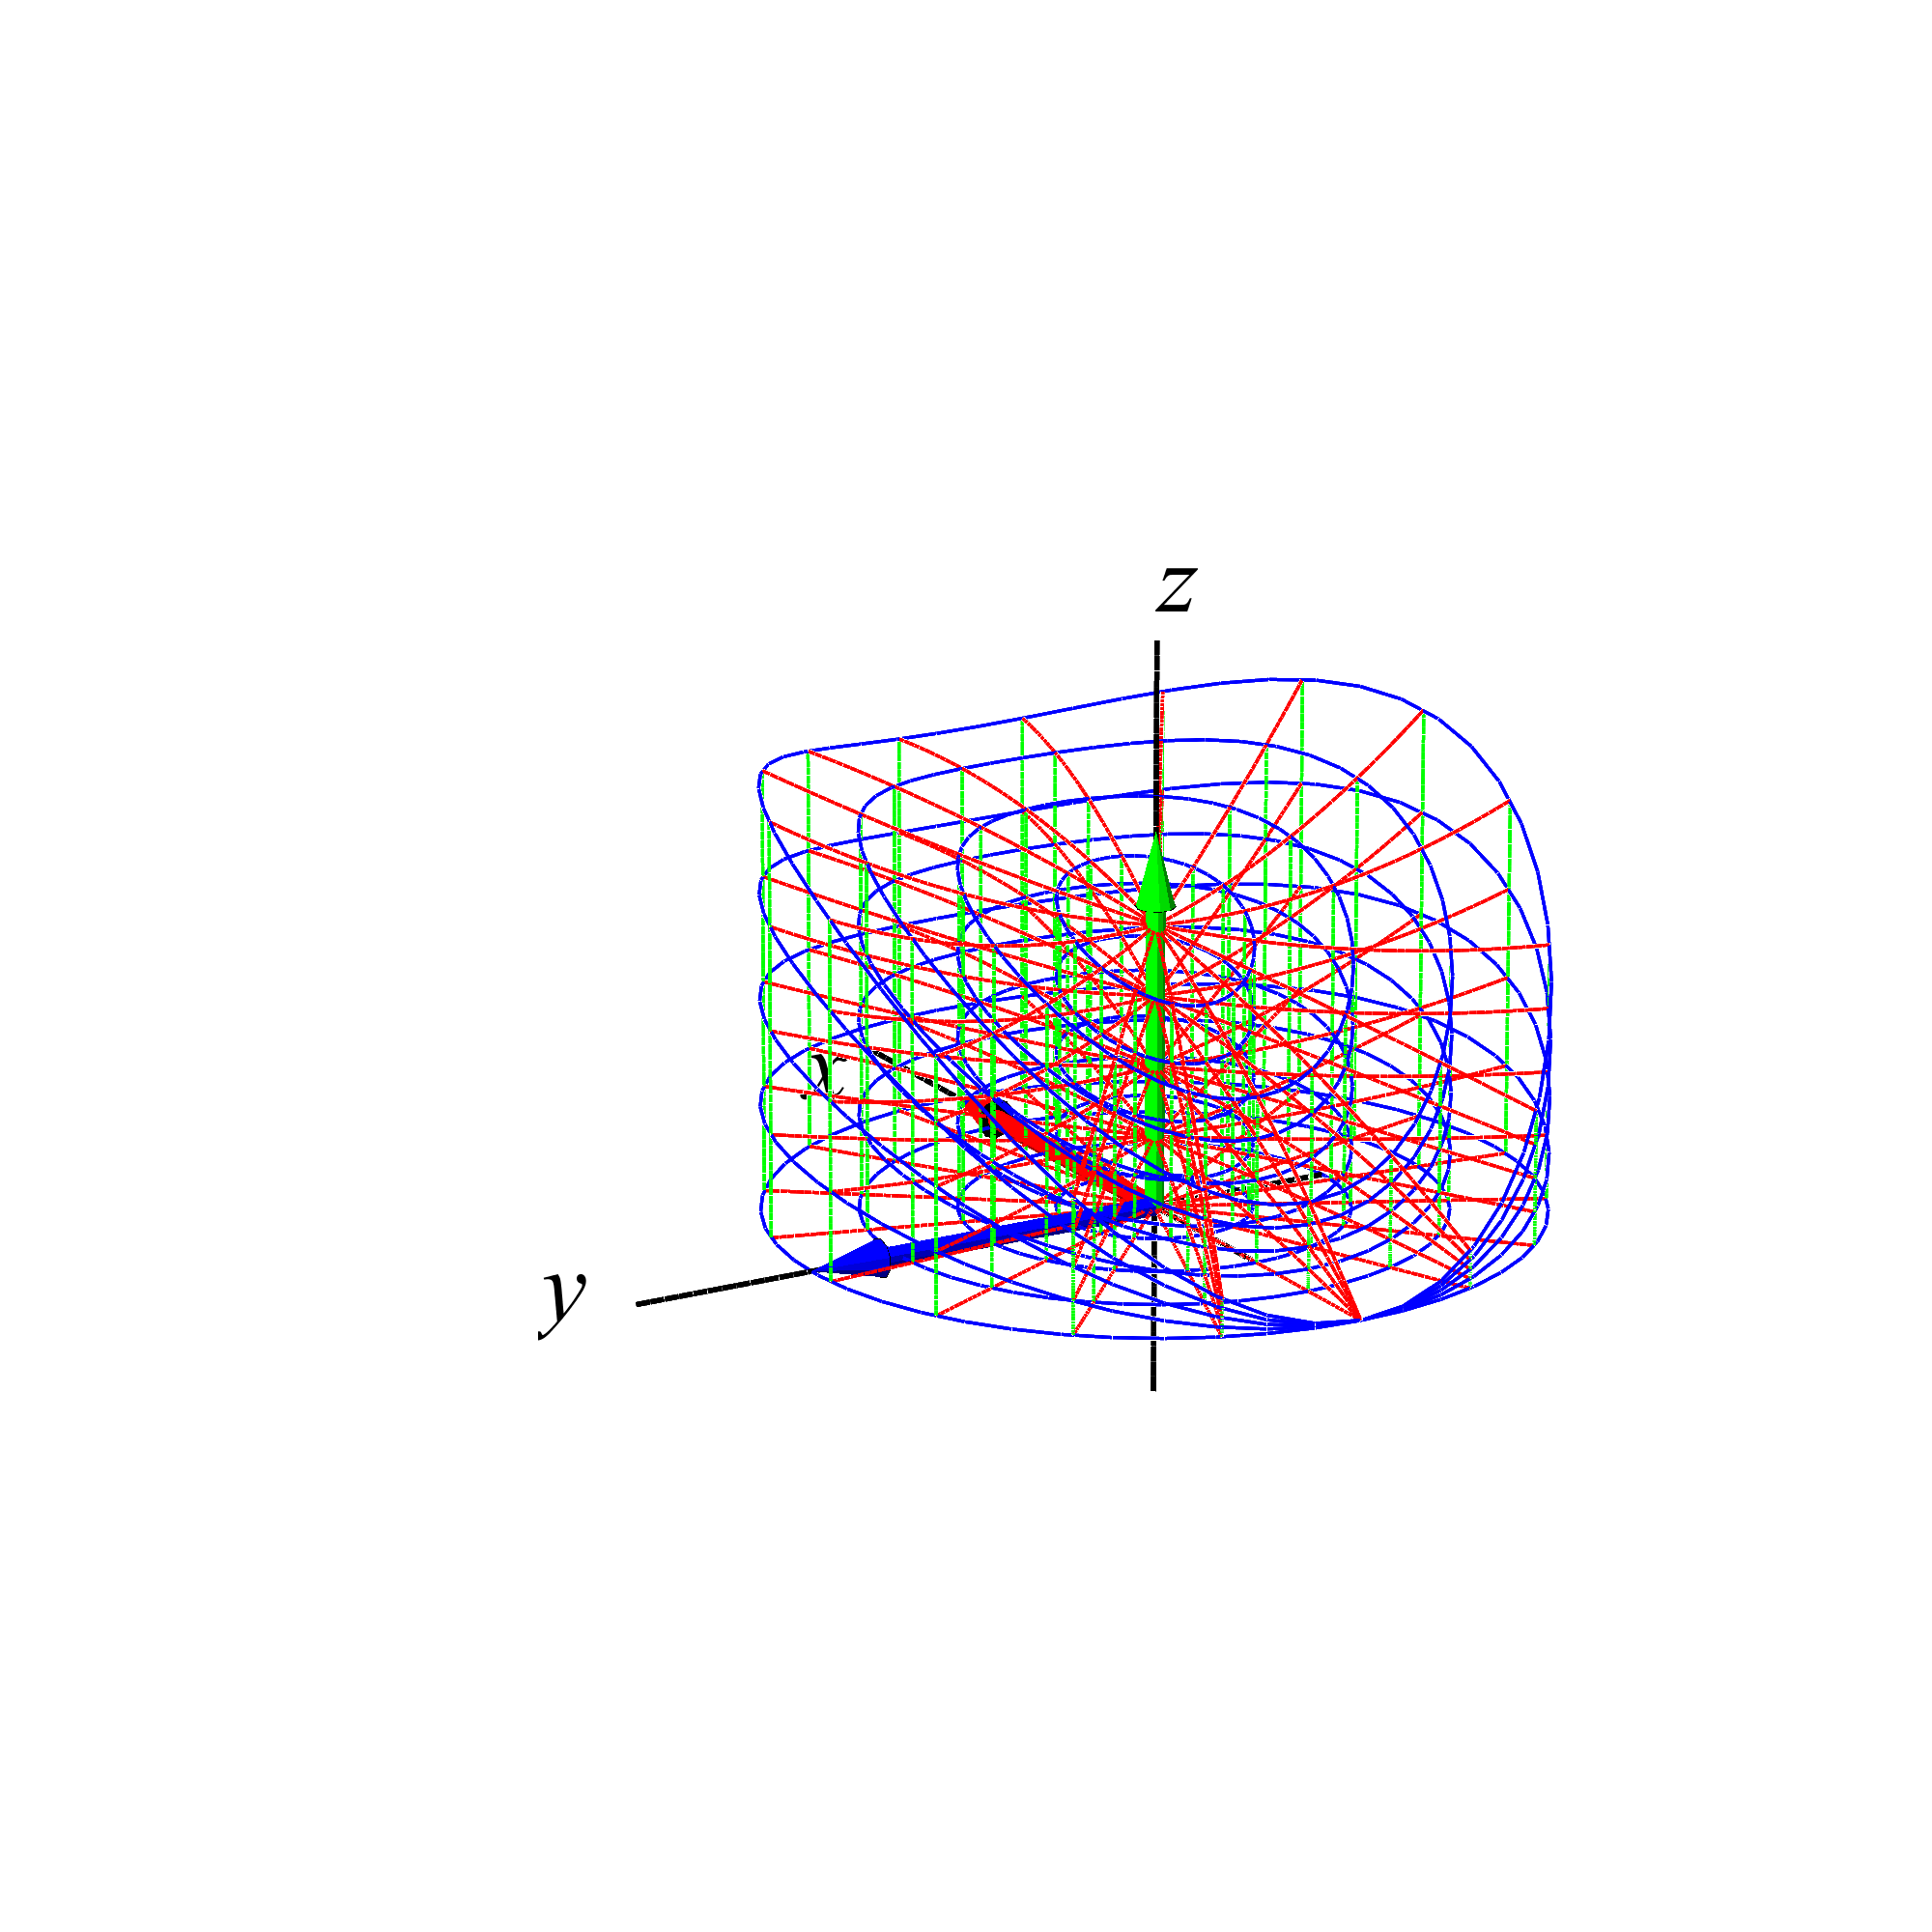
\includegraphics[height=70mm]{FIGS/plotGrafHypVol2} 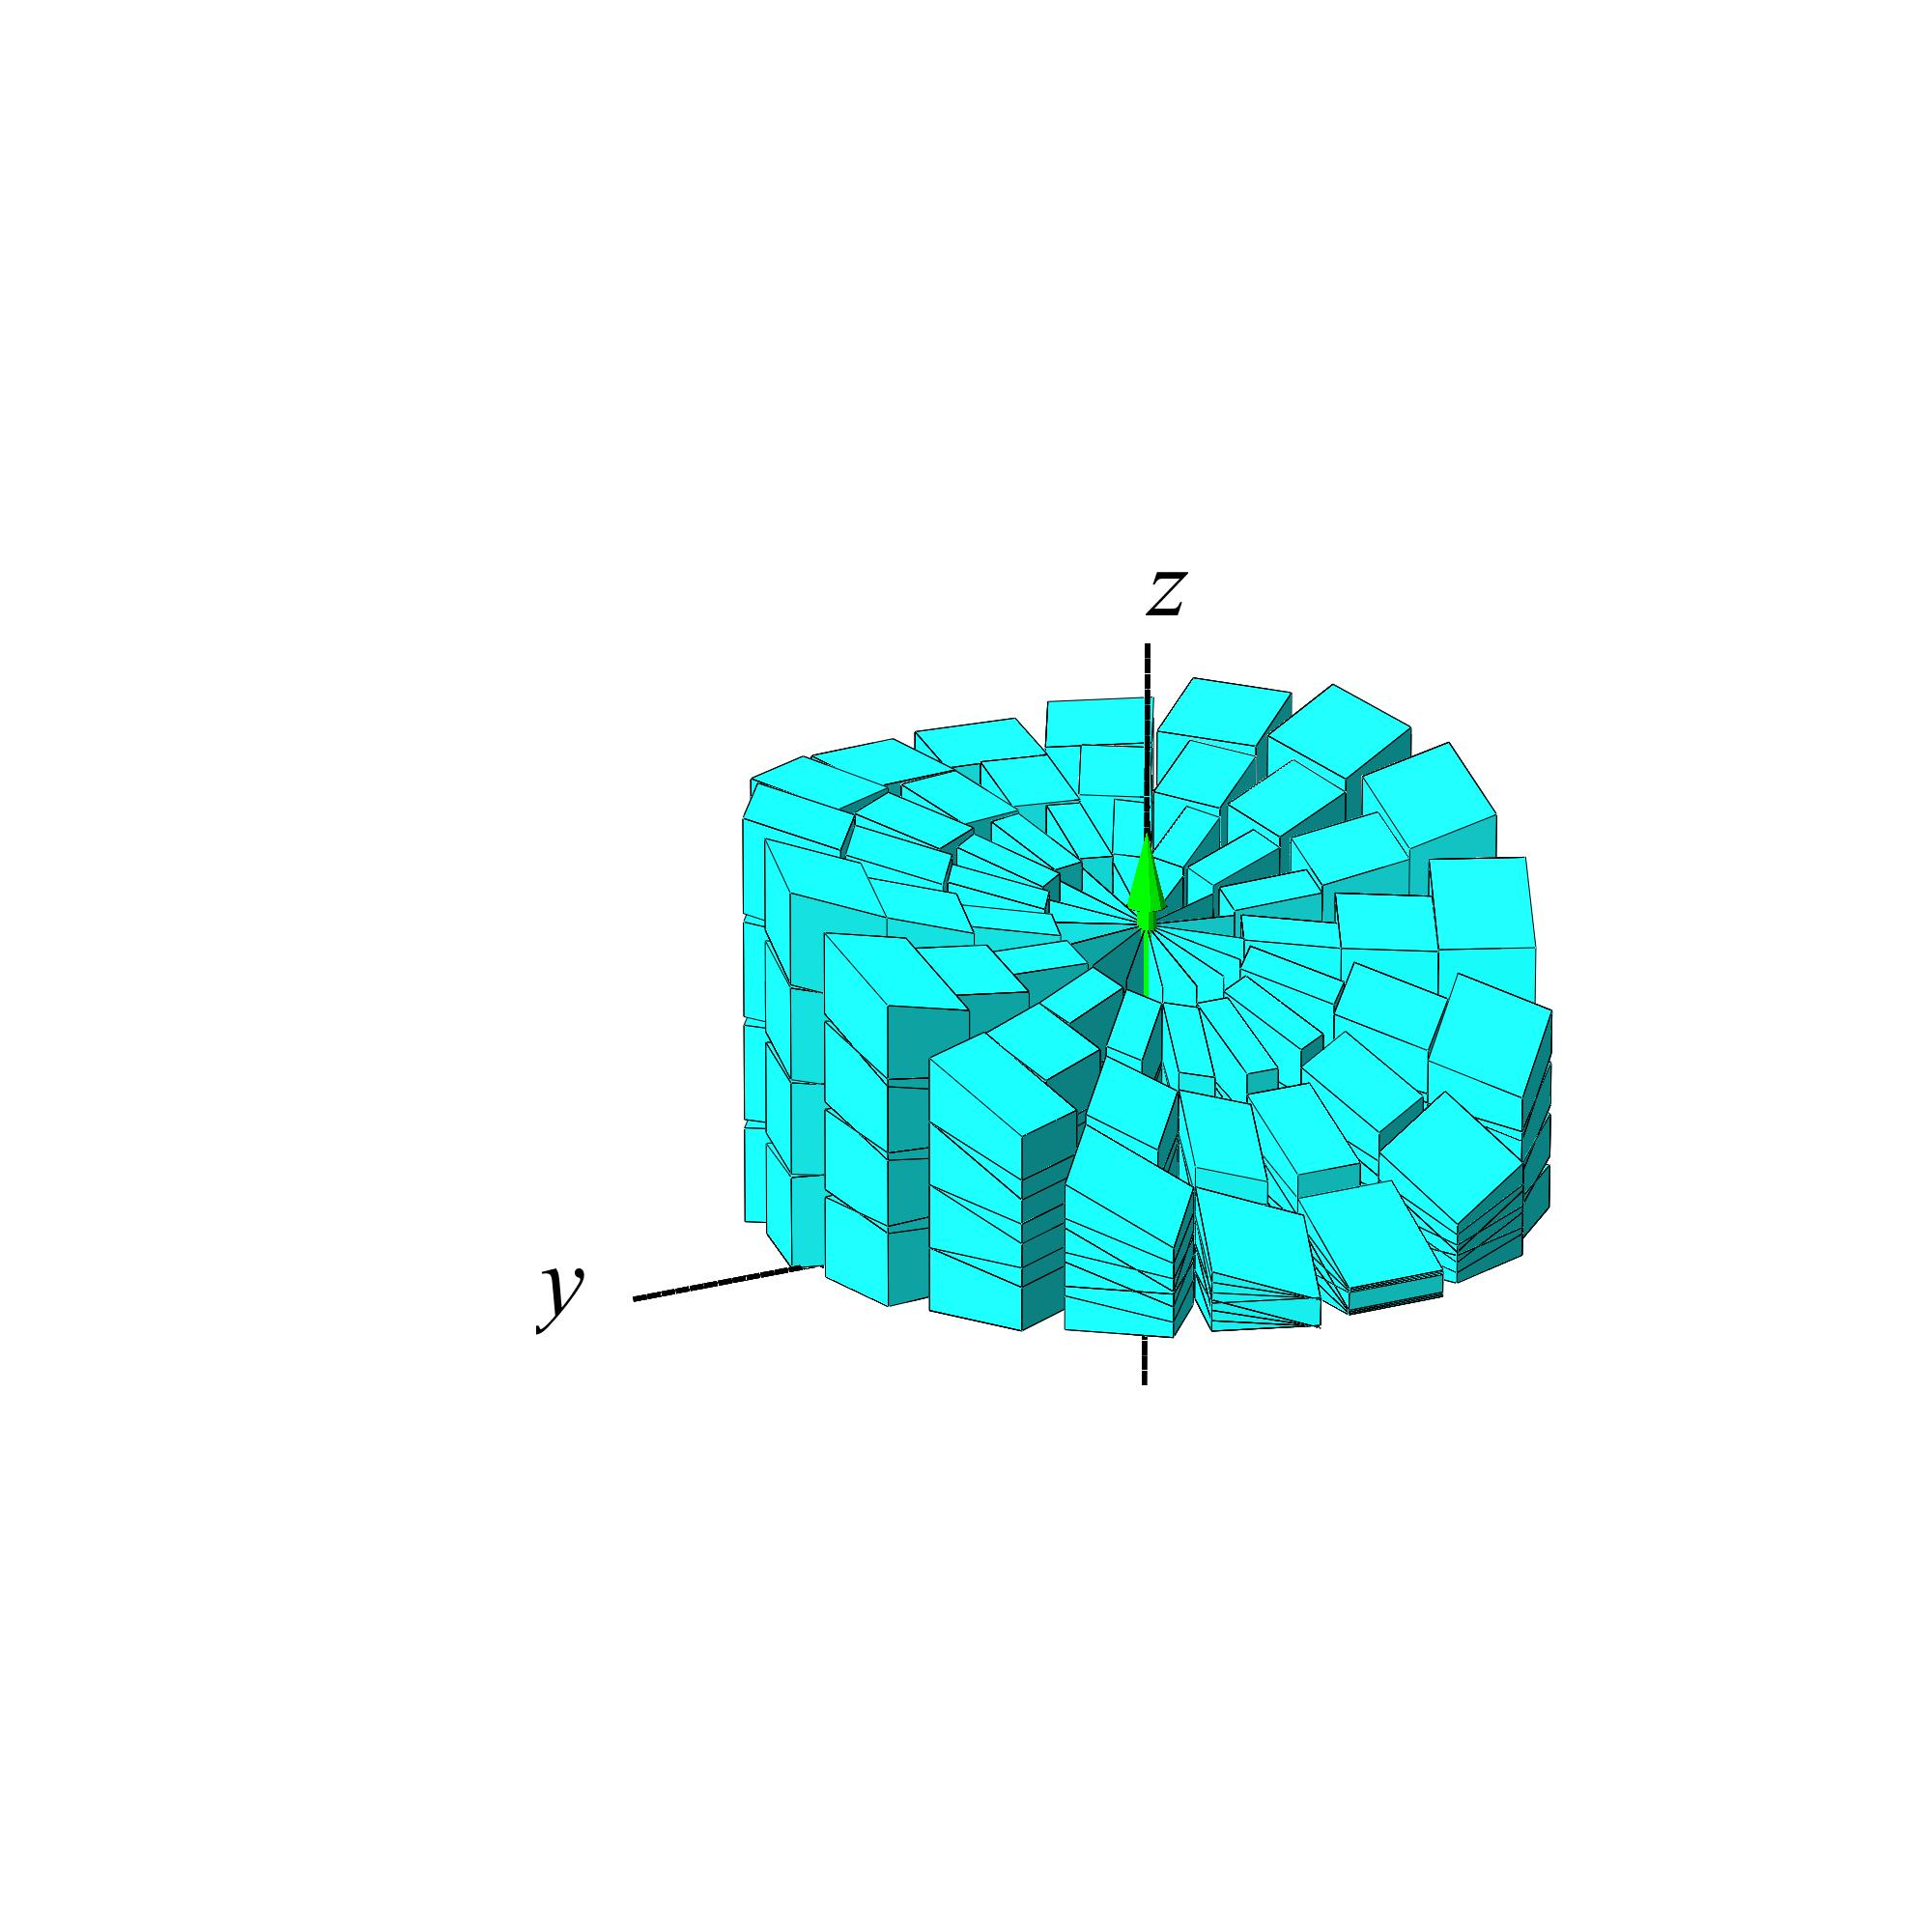
\includegraphics[height=70mm]{FIGS/plotGrafHypVol3}}
\begin{center}
\caption{\small{Et 'planetarium' med en lidt mere kompliceret tag-graf-flade; den benyttede funktion er her $f(x,y)= y^{2} - x^{2}+ 2x +3$. Rumfanget er ca. $2.36$.}}
\label{figGrafHypVol}
\end{center}
\end{figure}


\begin{example}[Planetariet]\label{exampPlanetarium}
Rumfanget i en cylinder mellem to plane afskæringer (se figur \ref{figGrafVol}) er bestemt ved para\-me\-ter\-frem\-stil\-lin\-gen:
\begin{equation}
\Omega_{\mathbf{r}} \quad : \quad \mathbf{r}(u,v,w) = (\xi(u,v), \eta(u,v), w\cdot h(\xi(u,v),\eta(u,v))) \quad ,
\end{equation}
hvor højdefunktionen er $h(x,y) = 2 - x- y$, parametrene er $(u,v) \in [0,1]\times[-\pi, \pi]$, $w \in [0, 1]$, og det cirkulære grundareal er givet ved
\begin{equation}
P \quad : \quad \widehat{\mathbf{r}}(u,v) = (u\cdot \cos(v), u\cdot \sin(v)) \quad , u \in [0,1] \quad , \quad v \in [-\pi, \pi]
\end{equation}
med Jacobi-funktionen
\begin{equation}
\Jac_{\widehat{\mathbf{r}}}(u,v) = u \quad ,
\end{equation}
således at
\begin{equation}
\begin{aligned}
\Vol(\Omega_{\mathbf{r}}) &= \int_{-\pi}^{\pi} \int_{0}^{1} h(\xi(u,v),\eta(u,v))\cdot \Jac_{\widehat{\mathbf{r}}}(u,v)  \,du
\, dv \\
&= \int_{-\pi}^{\pi} \int_{0}^{1} (2 - u\cdot \cos(v) -  u\cdot \sin(v))\cdot u \,du \, dv \\
&= \int_{-\pi}^{\pi} \int_{0}^{1} (2u - u^{2}\cdot \cos(v) -  u^{2}\cdot \sin(v)) \,du \, dv \\
&= \int_{-\pi}^{\pi} (\left[u^{2}\right]_{u=0}^{u=1} - \left[\frac{1}{3} u^{3} \right]_{u=0}^{u=1} \cdot \cos(v) -  \left[\frac{1}{3} u^{3} \right]_{u=0}^{u=1}\cdot \sin(v))\, dv \\
&=  \int_{-\pi}^{\pi} \left(1 - \frac{1}{3}\cdot \cos(v) -  \frac{1}{3}\cdot \sin(v)\right)\, dv \\
&= 2\cdot \pi \quad .
\end{aligned}
\end{equation}
Bemærk, at det rumfang også vha. symmetri kan findes meget lettere som halvdelen  af rumfanget af den cylinder, der har samme grundflade og er skåret vinkelret i højden $4$.
\end{example}





\section{Omdrejningslegemer} \label{subsecOmdrejningsLegemer}
{Omdrejningslegemer} er de specielle rumlige
områder, der fremkommer ved at dreje et plant
område (f.eks. defineret i $(x, z)$-planen)
omkring en omdrejningsakse i samme plan
($z$-aksen), som antages at ligge udenfor
området. Jævnfør de\-fi\-ni\-tionen af
om\-drej\-nings\-fla\-der i afsnit
\ref{subsecOmdrejningsflader}. \\

Det plane område - profilområdet - repræsenteres
ved en parameterfremstilling således:
\begin{equation}
P_{\bf r} : \quad {\bf r}(u,v) \, = \, \left(g(u,v), 0, h(u,v)\right)
\in \mathbb{R}^3 \quad , \, \, \,  u \in [a,b] \, \,
, \, \, v \in [c, d] \quad,
\end{equation}
hvor $g(u,v)\, > \, 0 $  og $h(u,v)$ er givne
funktioner af parametrene $u$ og $v$. Det rumlige
område, det legeme, der fremkommer ved at dreje
profilområdet en hel gang omkring $z$-aksen har
derfor parameterfremstillingen:
\begin{equation} \label{eqOmegaP}
\begin{aligned}
\Omega P_{\bf r} : &\quad {\bf r}(u,v,w) \, = \, \left(g(u,v)\cos(w), \, g(u,v)\sin(w),
\,
h(u,v)\right) \in \mathbb{R}^3 \quad ,  \\
 &u \in [a,b] \, \,
, \, \, v \in [c, d]  \, \,
, \, \, w \in [-\pi, \pi] \quad.
\end{aligned}
\end{equation}


Figur \ref{fig3d13} viser halvdelen af et omdrejningslegeme. Figur
\ref{figKugle13} viser overfladen af et omdrejningslegeme defineret
ved brug af kuglekoordinater. Cylinder-koordinater i rummet giver
tilsvarende velkendte omdrejningslegemer som f.eks. det, der er vist
i figur \ref{figCylinder123}.

\begin{figure}[h]
\centerline{\includegraphics[height=60mm]{FIGS/plotCylinder1}\includegraphics[height=60mm]{FIGS/plotCylinder2} \qquad\includegraphics[height=60mm]{FIGS/plotCylinder3}}
\begin{center}
\caption{\small{Cylinderkoordinatiseret rumligt område givet ved
parameterfremstillingen ${\bf r}(u, v, w) \, = \,
(g(u,v)\cos(w), \, g(u,v)\sin(w),\,  h(u,v) )
\,\,, \,\, u \in [0, \frac{1}{2} ]\,\, , \, \, v
\in [-\frac{1}{2}, \frac{1}{2}]\,\, , \, \, w \in
[-\pi, \pi] $, hvor $g(u,v) = u$ og $h(u,v)=v$.}}
\label{figCylinder123}
\end{center}
\end{figure}


\begin{exercise}
Vis, at Jacobifunktionen $\Jac_{{\bf r}}(u,v,w)$
for parameterfremstillingen ${\bf r}(u,v,w)$ for
det generelle omdrejningslegeme $\Omega P_{{\bf
r}}$ i (\ref{eqOmegaP}) er givet ved
\begin{equation}
\Jac_{{\bf r}}(u,v,w)\, = \, g(u, v)\,|
g'_{u}(u,v)\,h'_{v}(u,v) -
h'_{u}(u,v)\,g'_{v}(u,v)|  \quad .
\end{equation}
\end{exercise}


\begin{figure}[h]
\centerline{\includegraphics[height=70mm]{FIGS/plotBottle1} \includegraphics[height=70mm]{FIGS/plotDish1}}
\begin{center}
\caption{\small{Dele af henholdsvis omdrejnings-flaske og -fad, se Opgave \ref{excBottle}.}}
\label{figBottle}
\end{center}
\end{figure}



\begin{exercise} \label{excBottle}
En omdrejnings-flaske (eller -fad?) er (pånær bunden) givet ved sin profilkurves parameterfremstilling
i $(x, z)-$planen således:
\begin{equation}
G_{\bf r} : \quad {\bf r}(u) \, = \, \left(g(u), 0, h(u)\right)
\in \mathbb{R}^3 \quad , \, \, \,  u \in [0, 1] \quad,
\end{equation}
hvor
\begin{equation}
\begin{aligned}
g(u) \, &= \, 2(R_{1} - R_{2})u^{3} + 3(R_{2} - R_{1})u^{2} + R_{1} \\
h(u)\, &= \, H\,u \quad ,
\end{aligned}
\end{equation}
 for passende valg af {\em{positive}} konstanter $R_{1}$, $R_{2}$, og $H$.
\begin{enumerate}
\item Plot forskellige versioner af disse omdrejningsflader, se f.eks. figur \ref{figBottle}.
\item Vis, at omdrejningsfladen står vinkelret på $(x, y)-$planen for ethvert valg af positive konstanter $R_{1}$, $R_{2}$, og $H$.
\item Hvor meget rumfang (vand, f.eks.) kan omdrejningsfladen 'indeholde' for givne værdier af positive konstanter $R_{1}$, $R_{2}$, og $H$?
\item Hvad er arealet af overfladen af omdrejningsfladen + bund for givne værdier af positive konstanter $R_{1}$, $R_{2}$, og $H$?
\item Hvilke(t) valg af konstanter giver mest rumfang i forhold til det totale overfladeareal?
\end{enumerate}
\end{exercise}



\section{Flere arkitektonisk motiverede rumlige områder} \label{subsecAndreLegemer}

\begin{exercise}
Inspireret af Malmø's {Turning Torso} er det en interessant opgave at finde rumfang og overfladeareal af
forskellige 'snoede' bygningsværker:
\begin{enumerate}
\item Find en parameterfremstilling for det rumlige område, der er vist i figur \ref{figTurningTorso} til venstre. Vælg selv dimensionerne på din bygning, dvs. grundflade og højde. Vink: De opadgående sidelinjer er skruelinjer, se \tref{NUID37-exSkruelinje}{eksempel}   i \tref{NUID37-tn22}{eNote} .
\item Hvad er rumfanget af din bygning?
\item Hvad er overfladearealet af bygningens sidevægge?
\item Med fastholdt højde og tværsnitsfigur: Vis, at rumfanget er uafhængig af drejningstallet (det antal gange
tværsnitsfiguren drejes fra bund til top - for Torsoen er drejningstallet $1/5$). Hvordan afhænger overfladearealet af drejningstallet? Med hvilket drej\-nings\-tal fås det største volumen i forhold til det totale overfladeareal (af sidevæggene)?
\end{enumerate}
\end{exercise}

\begin{figure}[h]
\centerline{\includegraphics[height=95mm]{FIGS/plotTorso} \includegraphics[height=60mm]{FIGS/Turning_Torso_3}}
\begin{center}
\caption{\small{Fem-kantet Turning Torso model og 'the real thing in Malmø'.}}
\label{figTurningTorso}
\end{center}
\end{figure}


\begin{exercise}
Find parameterfremstillinger af de to (højeste) tårne der vises i figur \ref{figChinaCanada}.
Vælg selv dimensionerne. Vink: Tårnet i venstre billede har elliptiske tværsnit.
Find rumfang og overfladeareal for hver af bygningerne.
\end{exercise}

\begin{figure}[h]
\centerline{\includegraphics[height=60mm]{FIGS/ChinaCanadaMAD_tower_03} \includegraphics[height=60mm]{FIGS/CutOffTower}}
\begin{center}
\caption{\small{Chinese--Canadian projekt.}}
\label{figChinaCanada}
\end{center}
\end{figure}








%%%%%%%%%%%%%%%%%%%%%%%%%%%%%%%%%%%%%%%%%%%%%%%%%%%
%%%%%%%%%%%%%%%%%%%%%%%%%%%%%%%%%%%%%%%%%%%%%%%%%%%
%%%%%%%%%%%%%%%%%%%%%%%%%%%%%%%%%%%%%%%%%%%%%%%%%%%
%%%%%%%%%%%%%%%%%%%%%%%%%%%%%%%%%%%%%%%%%%%%%%%%%%%









%%%%%%%%%%%%%%%%%%%%%%%%%%%%%%%%%%%%%%%%%%%%%%%%%%%%%%%%%%%%%
%%%%%%%%%%%%%%%%%%%%%%%%%%%%%%%%%%%%%%%%%%%%%%%%%%%%%%%%%%%%%
%%%%%%%%%%%%%%%%%%%%%%%%%%%%%%%%%%%%%%%%%%%%%%%%%%%%%%%%%%%%%

\begin{summary}
Vi har i denne eNote opstillet de begreber og metoder der gør det muligt at beregne
(vægtede) arealer og rumfang af henholdsvis flader og rumlige områder -- for så vidt de er givet ved
parameterfremstillinger ud fra rektangulære og kasseformede  parameterområder. En række eksempler
og opgaver viser hvordan meget forskellige flader og områder kan parametriseres ved rimeligt simple
vektorfunktioner $\mathbf{r}(u,v)$ og $\mathbf{r}(u,v,w)$. \\

 Når først en relevant parametrisering er
opstillet er 'resten' kun et spørgsmål om at beregne den tilhørende Jacobifunktion $\Jac_{\mathbf{r}}(u,v)$ eller
$\Jac_{\mathbf{r}}(u,v,w)$, gange den med en eventuel vægtfunktion $f(x,y,z)$ restringeret til parametriseringens billedmængde i rummet, og til sidst beregne dobbelt- eller tredobbelt-
integralet af dette produkt over parameter-rektanglet eller parameter-kassen:
\begin{itemize}
\item For en flade $F_{\mathbf{r}}$ med parameterfremstillingen
\begin{equation}
F_{\bf r}: \quad {\bf r}(u,v) \, = \, \left(x(u,v), y(u,v),
z(u,v)\right) \in \mathbb{R}^3 \quad , \, \, \,  u \in [a,b] \, \,
, \, \,  v \in [c,d]
\end{equation}
er integralet af (vægt-)funktionen $f(x,y,z)$ over fladen givet ved:
\begin{equation}
\int_{F_{\bf r}} f \, d\mu \, = \, \int_{c}^{d} \int_{a}^{b}
f({\bf r}(u,v))\, \Jac_{\bf r}(u,v)\,du \, dv \quad,
\end{equation}
hvor {Jacobi-funktionen  $\Jac_{\bf r}(u,v)$}
\begin{equation}
 \Jac_{\bf r}(u,v)\, = \,  | {\bf r}'_{u}(u,v) \times {\bf
 r}'_{v}(u,v) |  \quad
\end{equation}
er arealet af det parallelogram, der på stedet
${\bf r}(u,v)$ udspændes af de to tangentvektorer
${\bf r}'_{u}(u,v)$ og ${\bf
 r}'_{v}(u,v)$ til de respektive koordinatkurver igennem punktet
${\bf r}(u,v)$ på fladen.
\item Specielt er arealet af $F_{\mathbf{r}}$ bestemt ved:
\begin{equation}
\Ar(F_{\bf r}) = \int_{F_{\bf r}} 1 \, d\mu = \int_{c}^{d} \int_{a}^{b} \Jac_{\bf r}(u,v)\,du \, dv \quad.
\end{equation}

\item For et rumligt område $\Omega_{\mathbf{r}}$ med parameterfremstillingen
\begin{equation}
\Omega_{\mathbf{r}}: \quad {\bf r}(u,v,w) \, = \, \left(x(u,v,w), y(u,v,w),
z(u,v,w)\right) \quad ,
\end{equation}
hvor $u \in [a,b]$, $v \in [c,d]$, og $w \in [h, l]$
er integralet af (vægt-)funktionen $f(x,y,z)$ over området givet ved:
\begin{equation}
\int_{\Omega_{\mathbf{r}}} f \, d\mu \, = \, \int_{h}^{l} \int_{c}^{d} \int_{a}^{b}
f({\bf r}(u,v,w))\, \Jac_{\bf r}(u,v,w)\,du \, dv \, dw \quad,
\end{equation}
hvor {Jacobi-funktionen  $\Jac_{\bf r}(u,v,w)$}
\begin{equation}
 \Jac_{\bf r}(u,v,w)\, = \,  | \left({\bf r}'_{u}(u,v,w) \times {\bf
 r}'_{v}(u,v,w)\right) \bm{\cdot} {\bf r}'_{w}(u,v,w)|  \quad
\end{equation}
er volumenet af det parallelepipedum, der på stedet
${\bf r}(u,v,w)$ udspændes af de tre tangentvektorer
${\bf r}'_{u}(u,v,w)$, ${\bf
 r}'_{v}(u,v,w)$, og ${\bf
 r}'_{w}(u,v,w)$ til de respektive koordinatkurver igennem punktet
${\bf r}(u,v,w)$ i det rumlige område.
\item Specielt er rumfanget af $\Omega_{\mathbf{r}}$ bestemt ved:
\begin{equation}
\Vol(\Omega_{\mathbf{r}}) = \int_{\Omega_{\mathbf{r}}} 1 \, d\mu = \int_{h}^{l} \int_{c}^{d} \int_{a}^{b} \Jac_{\bf r}(u,v,w)\,du \, dv \, dw \quad.
\end{equation}
\end{itemize}
\end{summary}


%%%%%%%%%%%%%%%%%%%%%%%%%%%%%%%%%%%%%%%%%%%%%
%%%%%%%%%%%%%%%%%%%%%%%%%%%%%%%%%%%%%%%%%%%%%
%%% HER SKAL DU STOPPE MED AT SKRIVE %%%%%%%%
%%%%%%%%%%%%%%%%%%%%%%%%%%%%%%%%%%%%%%%%%%%%%
%%%%%%%%%%%%%%%%%%%%%%%%%%%%%%%%%%%%%%%%%%%%%


\end{document} 

%%%%%%%%%%%%%%%%%%%%%%%%%%%%%%%%%%%%%%%%%%%%%%%%%%%
%%%%%%%%%%%%%%%%%%%%%%%%%%%%%%%%%%%%%%%%%%%%%%%%%%%

